\documentclass[12pt,a4paper]{report}
\usepackage[top=2.5cm,bottom=2.5cm,left=3cm,right=2.5cm]{geometry}
\usepackage{times}              
\usepackage[utf8]{inputenc}
\usepackage[T1]{fontenc}
\usepackage[bahasa]{babel}
\usepackage{graphicx}
\usepackage{amsmath,amssymb}
\usepackage{fancyhdr}
\usepackage[hidelinks]{hyperref}
\usepackage{enumitem}
\usepackage{array}
\usepackage{caption}
\usepackage{longtable}
\usepackage{booktabs}
\usepackage[utf8]{inputenc}
\usepackage[T1]{fontenc}
\usepackage{listings}
\usepackage{xcolor}
\usepackage{float}
\newcolumntype{L}[1]{>{\raggedright\arraybackslash}p{#1}}
\usepackage{titlesec}

\titleformat{\chapter}[hang]
  {\Large\bfseries}{\thechapter}{1em}{}
\titlespacing*{\chapter}{0pt}{0pt}{1.5em}

% section format
\titleformat{\section}
  {\large\bfseries}{\thesection}{1em}{}
\titlespacing*{\section}{0pt}{1.5em}{0.8em}

% subsection format
\titleformat{\subsection}
  {\normalsize\bfseries}{\thesubsection}{1em}{}
\titlespacing*{\subsection}{0pt}{1.2em}{0.6em}

% Header
\pagestyle{fancy}
\fancyhf{}
\fancyhead[L]{Kelompok Padang}
\fancyhead[R]{IF2123}
\fancyfoot[C]{\thepage}
\renewcommand{\headrulewidth}{0.4pt}
\renewcommand{\footrulewidth}{0pt}

\fancypagestyle{plain}{%
  \fancyhf{}%
  \fancyhead[L]{Kelompok Padang}%
  \fancyhead[R]{IF2123}%
  \fancyfoot[C]{\thepage}%
  \renewcommand{\headrulewidth}{0.4pt}%
}

\setlength{\parindent}{1.5em}
\setlength{\parskip}{0.5em}

\begin{document}

% Cover
\begin{titlepage}
\thispagestyle{empty}
\centering
\vspace*{1cm}

{\LARGE \textbf{Laporan Tugas Besar 1}\par}
\vspace{0.4cm}
{\Large \textbf{Sistem Persamaan Linier, Determinan, dan Penerapannya}\par}
\vspace{0.4cm}
{\large IF2123 Aljabar Linier dan Geometri\par}

\vfill

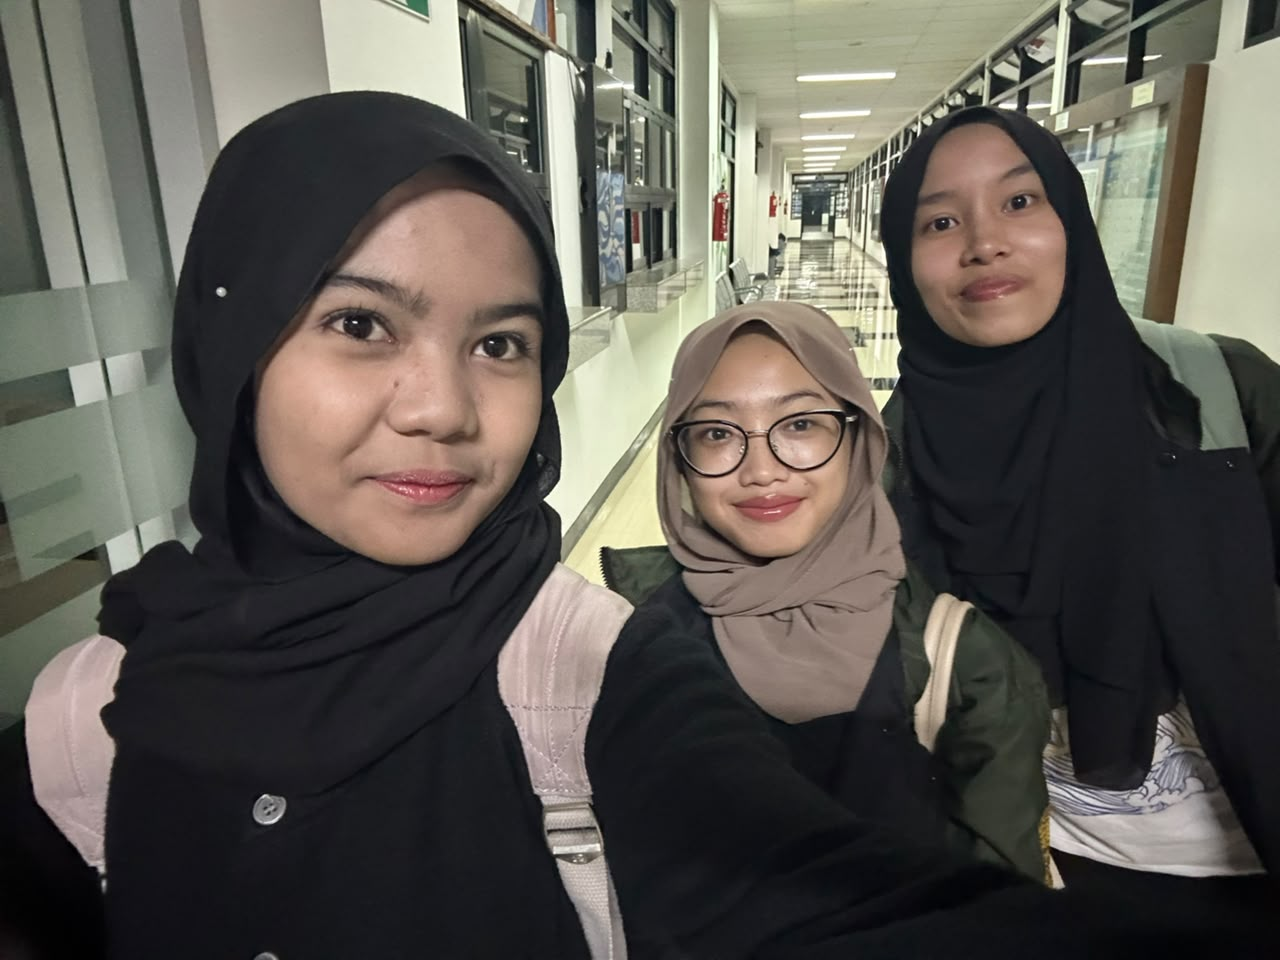
\includegraphics[width=8cm]{foto-kelompok.jpeg}

\vfill

{\large \textbf{Disusun oleh:}\par}
\vspace{0.5cm}
\begin{tabular}{ll}
Ghina Emelia Yantes     & 13525119 \\
Sahla Nailah Salsabilla & 13525134 \\
Nayla Putri Ghaisani    & 13525140 \\
\end{tabular}

\vfill

{\large Program Studi Teknik Informatika\par}
{\large Sekolah Teknik Elektro dan Informatika\par}
{\large Institut Teknologi Bandung\par}
{\large 2026\par}

\vspace*{1cm}
\end{titlepage}

% Daftar isi
\newpage
\renewcommand{\contentsname}{Daftar Isi}
\tableofcontents
\newpage

% BAB 1: PENDAHULUAN 
\chapter{Pendahuluan}

\section{Deskripsi Masalah}
Di pelosok Snezhnaya, seorang peneliti muda bernama Mitya tengah berusaha keras memimpin eksperimen krusial berskala raksasa: Proyek Stuzha. Proyek ini digadang-gadang mampu mengendalikan fluktuasi energi ekstrem di daratan Teyvat. Sayangnya, impian besar tersebut terbentur tembok tebal: Mitya masih mengandalkan kalkulator saku tua yang sering error tiap kali dipaksa menyelesaikan kalkulasi berdimensi tinggi.

\begin{figure}[htbp]
    \centering
    
\includegraphics[width=0.5\textwidth, height=8.5cm, keepaspectratio]{Picture3.jpg}
    \caption{Berkenalan dengan Mitya}
    \vspace{2pt} 
    {\small Sumber: Arsip Penulis}
    \label{fig:mitya}
\end{figure}

Setelah menjelajahi perpustakaan Sumeru Akademiya hingga menyisir kabar burung ke seantero Teyvat, Mitya mendengar reputasi kalian sebagai praktisi komputasi dan aljabar linier paling piawai. Ia pun mengirimkan pesan ke Adventures Guild dan memberikan komisi perangkat lunak sekelas Photomath versi Teyvat yaitu sebuah mesin kalkulasi otomatis yang sanggup melumat sistem matriks dan persamaan linier rumit demi kelangsungan Proyek Stuzha.

Aljabar linier bukan sekadar teori di atas kertas papirus; ini adalah fondasi komputasi modern yang menggerakkan simulasi rekayasa, pemodelan aliran energi, analisis data, hingga dinamika sistem kompleks. Agar kalkulasi Proyek Stuzha tidak runtuh di tengah jalan, kalian ditugaskan merancang dan membangun pustaka (\textit{library}) komputasi aljabar linier mandiri berbasis bahasa pemrograman \textbf{Java} yang modular, tangguh, dan terdokumentasi rapi.

\section{Latar Belakang}

Perkembangan teknologi rekayasa modern dan simulasi skala besar menuntut landasan komputasi yang tidak hanya akurat secara teoretis, tetapi juga tangguh dalam eksekusi praktis. Dalam perancangan sistem fisik yang kompleks, seperti pengoperasian infrastruktur pengendali energi ekstrem. Analisis matematis tidak lagi dapat diselesaikan secara manual atau menggunakan perangkat komputasi yang terbatas. Kompleksitas variabel yang saling terikat dalam jumlah besar menciptakan matriks dimensi tinggi yang rentan terhadap akumulasi galat jika ditangani dengan instrumen konvensional.

Kendala fundamental ini dihadapi dalam operasional Proyek Stuzha, di mana ketergantungan pada alat hitung konvensional yang usang memicu hambatan serius dalam validasi data dan pengujian kestabilan sistem. Kegagalan dalam menyelesaikan Sistem Persamaan Linier (SPL) berdimensi besar, perhitungan determinan, serta invers matriks secara presisi dapat berakibat fatal pada kalkulasi keseimbangan sirkuit daya. Oleh karena itu, diperlukan transisi menuju sistem komputasi terotomatisasi yang terstruktur.

Sebagai respons atas kebutuhan mendesak tersebut, pengembangan sebuah \textit{library} komputasi aljabar linier mandiri berbasis \textbf{Java} menjadi solusi arsitektural yang krusial. Pendekatan berbasis objek (\textit{object-oriented programming}) dipilih untuk memastikan modularitas kode, skalabilitas, dan kemudahan pemeliharaan. Pustaka ini dirancang untuk mengintegrasikan tiga pilar utama kebutuhan komputasi proyek:

\begin{enumerate}
    \item{Penyelesaian Aljabar Matriks dan SPL:} Sebagai kerangka dasar untuk menganalisis kestabilan instrumen dan distribusi daya secara simultan.
    \item{Metode Interpolasi dan Regresi Numerik:} Memungkinkan pemetaan jalur transfer energi serta pemodelan kontur data eksperimental yang bersifat non-linear dengan tingkat galat minimal.
\end{enumerate}

Melalui perancangan pustaka ini, implementasi teori aljabar linier ditransformasikan menjadi perangkat lunak yang andal, siap menghadapi skenario uji ekstrem, dan menjadi fondasi komputasi yang berkelanjutan bagi instrumen riset masa depan.

\section{Tujuan}
\begin{enumerate}
    \item Mengimplementasikan metode penyelesaian SPL, determinan, invers matriks, interpolasi polinomial, Natural Cubic Spline Interpolation, dan regresi Spline secara mandiri menggunakan Java.
    \item Membangun pustaka (library) aljabar linier yang terstruktur secara modular, bersih, dan terdokumentasi dengan baik. Tidak menggunakan library perhitungan matriks, regresi, atau interpolasi instan.
    \item Menguji keandalan pustaka pada berbagai kasus uji analitis dan restorasi citra, serta menyusun laporan analisis hasil perhitungannya.
 \end{enumerate}
 
% BAB 2: DASAR TEORI
\chapter{Dasar Teori}

\section{Sistem Persamaan Linear}
Sistem Persamaan Linear (SPL) adalah himpunan berhingga dari persamaan-persamaan linear dengan variabel-variabel yang sama. Bentuk umum dari SPL dengan $m$ persamaan dan $n$ variabel adalah

\[
\left\{
\begin{aligned}
a_{11}x_1 + a_{12}x_2 + a_{13}x_3 + \cdots + a_{1n}x_n &= b_1 \\
a_{21}x_1 + a_{22}x_2 + a_{23}x_3 + \cdots + a_{2n}x_n &= b_2 \\
&\;\;\dots \\
a_{n1}x_1 + a_{n2}x_2 + a_{n3}x_3 + \cdots + a_{nn}x_n &= b_n
\end{aligned}
\right.
\]

atau, dalam bentuk perkalian matriks (kiri) dan matriks augmented (kanan)

\[
\underbrace{
\begin{bmatrix}
a_{11} & a_{12} & \cdots & a_{1n} \\
a_{21} & a_{22} & \cdots & a_{2n} \\
\vdots & \vdots & \ddots & \vdots \\
a_{n1} & a_{n2} & \cdots & a_{nn}
\end{bmatrix}
}_{A}
\underbrace{
\begin{bmatrix}
x_1 \\
x_2 \\
\vdots \\
x_n
\end{bmatrix}
}_{x}
=
\underbrace{
\begin{bmatrix}
b_1 \\
b_2 \\
\vdots \\
b_n
\end{bmatrix}
}_{b}
\quad \rightarrow \quad
\begin{bmatrix}
a_{11} & a_{12} & \cdots & a_{1n} & b_1 \\
a_{21} & a_{22} & \cdots & a_{2n} & b_2 \\
\vdots & \vdots & \ddots & \vdots & \vdots \\
a_{n1} & a_{n2} & \cdots & a_{nn} & b_n
\end{bmatrix}
\]

Solusi dari SPL dapat berupa solusi tunggal, banyak solusi, atau tidak ada solusi. Metode penyelesaian yang umum digunakan antara lain eliminasi Gauss, eliminasi Gauss-Jordan, kaidah Cramer, dan metode matriks balikan.
\subsection{Metode Eliminasi Gauss}
Eliminasi Gauss adalah metode penyelesaian sistem persamaan linear dengan mengubah matriks augmented ke bentuk eselon baris, lalu mencari nilai variabel menggunakan \textit{substitusi mundur}. Langkah-langkah utamanya meliputi:
\begin{enumerate}
    \item Menyusun sistem persamaan linear ke dalam bentuk matriks augmented $[A \mid b]$.
    \item Melakukan Operasi Baris Elementer (OBE) melalui fase \textit{eliminasi maju} (\textit{forward elimination}) hingga elemen di bawah diagonal utama bernilai nol (membentuk matriks segitiga atas).
    \item Menerapkan proses \textit{substitusi mundur} (\textit{back-substitution}) dari baris paling bawah ke atas untuk mendapatkan nilai setiap variabel ($x_1, x_2, \dots, x_n$).
\end{enumerate}

\subsection{Metode Eliminasi Gauss-Jordan}
Eliminasi Gauss-Jordan merupakan pengembangan lanjutan dari eliminasi Gauss. Metode ini menambahkan fase eliminasi mundur di dalam operasi baris sehingga matriks berubah menjadi bentuk eselon baris tereduksi (matriks identitas). Langkah-langkahnya meliputi:
\begin{enumerate}
    \item Menyusun sistem persamaan linear ke dalam bentuk matriks augmented $[A \mid b]$.
    \item Melakukan eliminasi maju untuk membentuk segitiga atas.
    \item Melanjutkan eliminasi mundur (masih menggunakan OBE) untuk membuat elemen di atas diagonal utama bernilai nol dan diagonal utamanya bernilai satu.
    \item Nilai variabel atau solusi akhir dapat langsung dibaca dari kolom terakhir matriks tanpa perlu melalui proses substitusi mundur manual.
\end{enumerate}

\subsection{Metode Matriks Balikan}
Metode matriks balikan (invers) digunakan untuk menyelesaikan sistem persamaan linear yang dapat direpresentasikan dalam bentuk persamaan matriks $AX = B$. Langkah-langkah utamanya meliputi:
\begin{enumerate}
    \item Mengubah sistem persamaan linear ke dalam bentuk matriks $AX = B$, di mana $A$ adalah matriks koefisien, $X$ adalah matriks variabel, dan $B$ adalah matriks konstanta.
    \item Memastikan bahwa matriks $A$ adalah matriks persegi dan memiliki balikan (invers), yaitu determinan $A \neq 0$.
    \item Menghitung invers dari matriks $A$ ($A^{-1}$).
    \item Mendapatkan nilai variabel dengan mengalikan invers matriks $A$ dengan matriks konstanta $B$ melalui rumus $X = A^{-1}B$.
\end{enumerate}

\subsection{Kaidah Cramer}
Kaidah Cramer adalah metode penyelesaian sistem persamaan linear menggunakan konsep determinan matriks. Metode ini efektif untuk sistem dengan ukuran kecil ($2 \times 2$ atau $3 \times 3$). Langkah-langkah utamanya meliputi:
\begin{enumerate}
    \item Menyusun sistem persamaan linear ke dalam bentuk matriks $AX = B$.
    \item Menghitung determinan dari matriks koefisien $A$, yaitu $\det(A)$, dengan syarat $\det(A) \neq 0$.
    \item Membentuk matriks $A_i$ dengan cara mengganti kolom ke-$i$ pada matriks $A$ dengan matriks konstanta $B$, lalu menghitung determinannya ($\det(A_i)$) untuk setiap variabel.
    \item Menentukan nilai setiap variabel ($x_i$) menggunakan rumus:
    \[
    x_i = \frac{\det(A_i)}{\det(A)}
    \]
\end{enumerate}

\section{Determinan Matriks}
Determinan adalah sebuah nilai skalar khusus yang dapat dihitung dari elemen-elemen sebuah matriks persegi. Determinan dari matriks $A$ dinotasikan sebagai $\det(A)$ atau $|A|$. Nilai determinan sangat krusial karena dapat mengindikasikan apakah matriks tersebut memiliki invers. Beberapa metode untuk menghitung determinan matriks mencakup metode ekspansi kofaktor dan metode reduksi baris (OBE).


\subsection{Determinan Kofaktor}
Determinan kofaktor (atau ekspansi kofaktor) adalah metode menghitung determinan matriks persegi dengan cara mengembangkannya sepanjang baris atau kolom tertentu. Langkah-langkah dan konsep utamanya meliputi:
\begin{enumerate}
    \item Memilih baris atau kolom tertentu pada matriks $A$ (biasanya dipilih yang memiliki banyak unsur nol untuk mempermudah perhitungan).
    \item Menghitung minor ($M_{ij}$), yaitu determinan dari submatriks berukuran $(n-1) \times (n-1)$ yang diperoleh dengan menghapus baris ke-$i$ dan kolom ke-$j$ dari matriks $A$.
    \item Menentukan kofaktor $C_{ij}$ melalui rumus:
    \[
    C_{ij} = (-1)^{i+j} M_{ij}
    \]
    \item Menjumlahkan hasil kali setiap elemen pada baris atau kolom pilihan dengan kofaktorkannya. Sebagai contoh, ekspansi sepanjang baris pertama dirumuskan sebagai:
    \[
    \det(A) = a_{11}C_{11} + a_{12}C_{12} + a_{13}C_{13} + \dots + a_{1n}C_{1n}
    \]
\end{enumerate}

\subsection{Determinan Reduksi Baris (OBE)}
Determinan reduksi baris adalah metode menghitung determinan dengan mereduksi matriks persegi menjadi bentuk matriks segitiga atas menggunakan Operasi Baris Elementer (OBE). Metode ini jauh lebih efisien untuk matriks berukuran besar. Aturan perubahan nilai determinan akibat OBE meliputi:
\begin{enumerate}
    \item Pertukaran baris: Jika dua baris matriks ditukar posisinya, maka nilai determinan akan bertanda berlawanan (dikalikan dengan $-1$).
    \item Perkalian baris dengan skalar: Jika seluruh elemen pada suatu baris dikalikan dengan skalar $k$, maka determinan matriks baru menjadi $k$ kali determinan semula.
    \item Penjumlahan kelipatan baris: Menambahkan kelipatan suatu baris ke baris lainnya tidak mengubah nilai determinan sama sekali.
\end{enumerate}
Setelah matriks berhasil diubah menjadi bentuk segitiga atas (elemen di bawah diagonal utama bernilai nol), determinan dapat dihitung dengan mudah melalui hasil kali seluruh elemen pada diagonal utamanya:
\[
\det(A) = a_{11} a_{22} a_{33} \dots a_{nn}
\]
\section{Invers Matriks}
Invers dari sebuah matriks persegi $A$ adalah matriks $A^{-1}$ yang memenuhi properti $AA^{-1} = A^{-1}A = I$, di mana $I$ adalah matriks identitas. Sebuah matriks hanya memiliki invers jika dan hanya jika determinannya tidak nol ($\det(A) \neq 0$). Matriks yang memiliki invers disebut matriks \textit{invertible} atau non-singular. Perhitungan invers dari suatu matriks dapat dilakukan dengan metode matriks adjoin maupun metode eliminasi Gauss-Jordan.

\subsection{Inverse Augmented}
Invers matriks menggunakan metode augmented (atau eliminasi Gauss-Jordan) dilakukan dengan mereduksi matriks asal berdampingan dengan matriks identitas. Langkah-langkahnya meliputi:
\begin{enumerate}
    \item Menuliskan matriks augmented yang menggabungkan matriks $A$ dan matriks identitas $I$ dengan bentuk $[\begin{array}{c|c} A & I \end{array}]$.
    \item Melakukan Operasi Baris Elementer (OBE) pada seluruh baris matriks augmented tersebut.
    \item Melanjutkan OBE hingga sisi kiri matriks yang awalnya berupa matriks $A$ berubah sepenuhnya menjadi matriks identitas $I$.
    \item Membaca hasil akhir pada sisi kanan matriks augmented, di mana bagian tersebut secara otomatis telah berubah menjadi matriks invers ($A^{-1}$), sehingga bentuk akhirnya menjadi $[\begin{array}{c|c} I & A^{-1} \end{array}]$.
\end{enumerate}

\subsection{Inverse Adjoint}
Invers matriks menggunakan adjoin dihitung dengan memanfaatkan nilai determinan dan matriks kofaktor dari suatu matriks persegi. Langkah-langkahnya meliputi:
\begin{enumerate}
    \item Menghitung determinan matriks $A$, yaitu $\det(A)$, dan memastikan bahwa $\det(A) \neq 0$ agar matriks tersebut memiliki invers.
    \item Menentukan matriks kofaktor dari $A$ dengan mencari kofaktor untuk setiap elemen matriks tersebut.
    \item Menentukan matriks adjoin, yaitu $\text{adj}(A)$, dengan cara mentranspose-kan matriks kofaktor yang telah diperoleh.
    \item Menghitung invers matriks $A$ menggunakan rumus:
    \[
    A^{-1} = \frac{1}{\det(A)} \text{adj}(A)
    \]
\end{enumerate}

\section{Interpolasi Polinomial}
Interpolasi polinomial adalah metode untuk menentukan suatu polinomial $P_n(x)$ berderajat $n$ yang melalui $n+1$ titik data $(x_0, y_0), (x_1, y_1), \dots, (x_n, y_n)$, $x_i$ diurutkan dengan $x_0$ terkecil dan $x_n$ terbesar. Secara umum, polinomial tersebut dapat dituliskan sebagai:

\[
P_n(x) = a_0 + a_1x + a_2x^2 + \cdots + a_nx^n
\]

dengan koefisien $a_0, a_1, \dots, a_n$ yang ditentukan sedemikian rupa sehingga $P_n(x_{\text{perkiraan}}) = y_{\text{perkiraan}}$ untuk semua nilai $x_0 < x_{\text{perkiraan}} < x_n$. Derajat persamaan polynom ditentukan oleh jumlah titik data yang diberikan dikurangi satu.

Koefisien polinomial dapat dicari dengan menyulihkan titik-titik data ke dalam persamaan polinomial dan menyelesaikan sistem persamaan linear yang dihasilkan dengan metode eliminasi Gauss yang dijelaskan sebelumnya. Kita dapat menyusun sistem persamaan linear sebagai berikut.
o
\[
\left\{
\begin{aligned}
a_0 + a_1x_0 + a_2x_0^2 + \cdots + a_nx_0^n &= y_0 \\
a_0 + a_1x_1 + a_2x_1^2 + \cdots + a_nx_1^n &= y_1 \\
&\;\;\vdots \\
a_0 + a_1x_n + a_2x_n^2 + \cdots + a_nx_n^n &= y_n
\end{aligned}
\right.
\]

Persamaan-persamaan di atas dapat dipetakan menjadi sebuah permasalahan sistem persamaan linear, sehingga dapat diselesaikan dengan menggunakan metode eliminasi Gauss untuk menyelesaikan

\begin{figure}
        \centering
    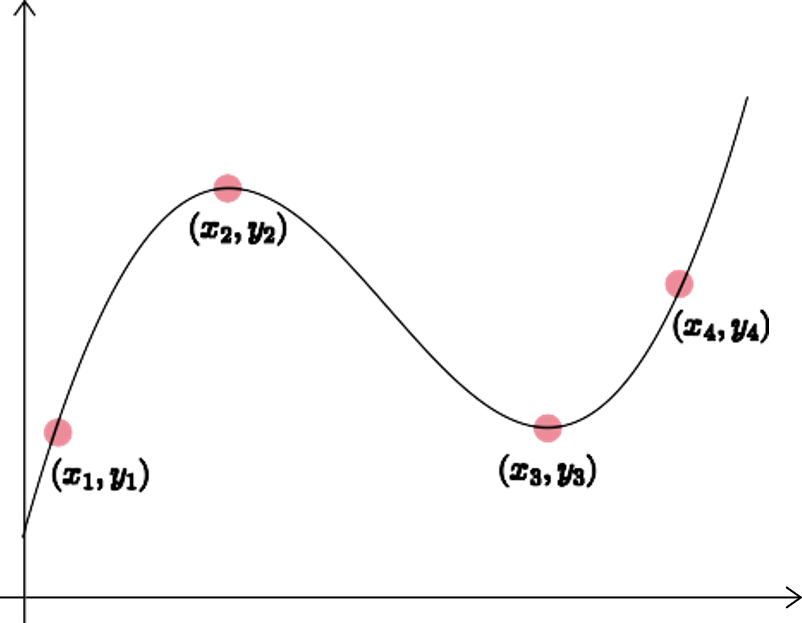
\includegraphics[width=0.5\linewidth]{Picture1.png}
        \caption{Gambar 2: Contoh interpolasi polinomial melalui empat titik data.}
    \label{fig:interpolasi_polinomial}
\end{figure}

\noindent sistem tersebut dan menemukan koefisien polinomial $a_0, a_1, \dots, a_n$. Dari polynom $P_n(x)$ yang dibentuk dengan koefisien tersebut, kita dapat memperkirakan nilai $y$ untuk nilai $x$ yang berada di antara titik-titik data yang diberikan (interpolasi) maupun di luar titik-titik data tersebut (ekstrapolasi).

\section{Natural Cubic Spline Interpolation}

\textit{Interpolasi Spline Kubik} (\textit{Cubic Spline Interpolation}) adalah metode interpolasi yang mengonstruksi kurva mulus melalui sekumpulan titik data diskret menggunakan potongan-potongan polinomial berderajat tiga (kubik) di setiap interval antar-titik. Berbeda dengan interpolasi polinomial tunggal orde tinggi yang rentan mengalami osilasi liar di ujung interval, \textit{spline} menjaga kelengkungan kurva tetap stabil dan kontinu hingga turunan kedua.

\begin{figure}
        \centering
        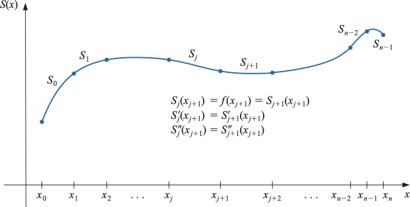
\includegraphics[width=0.5\linewidth]{Picture2.jpg}
        \caption{Gambar : Contoh Interpolasi Spline Kubik}
        {\small Sumber: R. L. Burden \& J. D. Faires, \textit{Numerical Analysis}}
    \label{fig:spline_kubik}
\end{figure}

Definisi dari \textit{cubic spline interpolation} $S$ untuk sebuah fungsi $f$ yang terdefinisi di $[a, b]$ dengan sekumpulan titik data \textbf{terurut} $a = x_0 < x_1 < \dots < x_n = b$ memenuhi kondisi berikut:

\begin{enumerate}[label=\alph*.]
    \item $S(x)$ merupakan potongan polinomial kubik $S_j(x)$ pada setiap subinterval $[x_j, x_{j+1}]$ untuk setiap $j = 0, 1, \dots, n-1$ (terdapat $n$ subinterval).
    \item $S_j(x_j) = f(x_j)$ dan $S_j(x_{j+1}) = f(x_{j+1})$ untuk setiap $j = 0, 1, \dots, n-1$.\\
    (Kurva harus melalui nilai fungsi pada titik-titik ujung tiap subinterval).
    \item $S_{j+1}(x_{j+1}) = S'{j}(x_{j+1})$ untuk setiap $j = 0, 1, \dots, n-2$. \\ (Kurva bersambung secara kontinu tanpa putus di setiap simpul interior).
    \item $S'_{j+1}(x_{j+1}) = S"{j}(x_{j+1})$ untuk setiap $j = 0, 1, \dots, n-2$. \\ (Kemiringan kurva dari sisi kiri dan kanan bernilai sama di setiap simpul interior).
    \item $S"_{j+1}(x_{j+1}) = S"{j}(x_{j+1})$ untuk setiap $j = 0, 1, \dots, n-2$. \\ (Kelengkungan (curvature) kurva dari sisi kiri dan kanan bernilai sama di setiap simpul interior).
    \item $S"_(x_{0}) = S"(x_{n})$ untuk \textit{natural spline}. \\ (Kurva tidak memiliki gaya lentur pada kedua ujung terluar sehingga berperilaku menyerupai garis lurus di luar rentang data).
    
\end{enumerate} Penjelasan matematis lebih mendalam mengenai penurunan rumus, pembentukan sistem persamaan tridiagonal, serta visualisasi grafik interpolasi spline kubik dapat dirujuk pada buku Numerical Analysis karya Burden dan Faires.

\subsection{Tridiagonal Matrix System for Cubic Splines}
Untuk menentukan kurva kubik yang mulus, turunan kedua pada setiap titik data ($z_i = S''(x_i)$) dihitung melalui suatu sistem persamaan linear khusus yang membentuk matriks tridiagonal. Sistem ini dirumuskan sebagai berikut:
\begin{enumerate}
    \item Persamaan kontinuitas turunan pertama antar segmen polinomial menghasilkan hubungan antarnilai turunan kedua:
    \[
    h_{i-1} z_{i-1} + 2(h_{i-1} + h_i) z_i + h_i z_{i+1} = 6 \left( \frac{y_{i+1} - y_i}{h_i} - \frac{y_i - y_{i-1}}{h_{i-1}} \right)
    \]
    di mana $h_i = x_{i+1} - x_i$ adalah jarak antar titik data.
    \item Untuk \textit{natural cubic spline}, nilai turunan kedua pada ujung-ujung interval bernilai nol ($z_0 = 0$ dan $z_n = 0$).
    \item Sistem persamaan linear di atas dapat direpresentasikan dalam bentuk matriks tridiagonal $Hz = b$:
    \[
    \begin{pmatrix}
    2(h_0 + h_1) & h_1 & 0 & \dots & 0 \\
    h_1 & 2(h_1 + h_2) & h_2 & \dots & 0 \\
    \vdots & \vdots & \vdots & \ddots & \vdots \\
    0 & 0 & \dots & h_{n-2} & 2(h_{n-2} + h_{n-1})
    \end{pmatrix}
    \begin{pmatrix}
    z_1 \\ z_2 \\ \vdots \\ z_{n-1}
    \end{pmatrix}
    =
    \begin{pmatrix}
    d_1 \\ d_2 \\ \vdots \\ d_{n-1}
    \end{pmatrix}
    \]
    \item Matriks koefisien di atas bersifat tridiagonal (hanya elemen pada diagonal utama, super-diagonal, dan sub-diagonal yang tidak bernilai nol), sehingga dapat diselesaikan secara sangat efisien menggunakan algoritma eliminasi Gauss khusus (seperti algoritma Thomas).
\end{enumerate}
\section{Splines Regression}

\textit{Splines Regression} adalah metode pemodelan non-parametrik yang memetakan hubungan non-linear antara variabel prediktor $x$ dan variabel respons $y$ menggunakan kombinasi potongan polinomial terhubung pada simpul-simpul tertentu (\textit{knots}), disimbolkan dengan $\xi_1 < \xi_2 < \dots < \xi_K$. Berbeda dari interpolasi yang menyelesaikan SPL deterministik untuk menghubungkan turunan pada setiap titik data, pendekatan \textit{splines regression} mentranslasikan permasalahan ke dalam Sistem Persamaan Linear \textit{Overdetermined} (jumlah data $N >$ jumlah basis $M$) melalui kerangka ruang fungsi basis, kemudian diselesaikan menggunakan Metode Kuadrat Terkecil (\textit{Ordinary Least Squares}).

\subsection*{1. Konstruksi Ruang Fungsi dan Basis Daya Terpancung (\textit{Truncated Power Basis})}
Ruang fungsi spline kubik dengan $K$ simpul internal $\xi_1, \xi_2, \dots, \xi_K$ merupakan ruang vektor berdimensi $M = 4 + K$, di mana 4 adalah jumlah koefisien polinomial kubik standar dan $K$ adalah jumlah fungsi basis tambahan untuk setiap simpul.

Setiap fungsi $f(x)$ dalam ruang tersebut dapat dinyatakan sebagai kombinasi linear unik dari $M$ buah fungsi basis $\{h_0(x), h_1(x), h_2(x), h_3(x), \dots, h_{3+K}(x)\}$:

Polinomial standar global:
\[
h_0(x) = 1, \quad h_1(x) = x, \quad h_2(x) = x^2, \quad h_3(x) = x^3
\]

Basis tambahan di setiap simpul $\xi_k$:
\[
h_{3+k}(x) = (x - \xi_k)_+^3 = 
\begin{cases}
(x - \xi_k)^3, & \text{jika } x > \xi_k \\
0, & \text{jika } x \le \xi_k
\end{cases}
\quad \text{untuk } k = 1, 2, \dots, K
\]

Fungsi regresi menjadi:
\[
f(x) = \sum_{j=0}^{3+K} \beta_j h_j(x) = \beta_0 + \beta_1 x + \beta_2 x^2 + \beta_3 x^3 + \sum_{k=1}^{K} \beta_{3+k} (x - \xi_k)_+^3
\]

Sifat kontinuitas turunan hingga $C^2$ di seluruh rentang $x$ langsung terpenuhi secara analitis oleh bentuk fungsi basis $(x - \xi_k)_+^3$ tanpa memerlukan penambahan persamaan batas turunan manual.

\textit{Catatan notasi:}
\[
(u)_+ = \max(0, u) = 
\begin{cases}
u, & \text{jika } u > 0 \\
0, & \text{jika } u \le 0
\end{cases}
\]

\subsection*{2. Formulasi Matriks Desain ($X\boldsymbol{\beta} \approx \mathbf{y}$)}
Diberikan $N$ sampel data pengamatan $(x_1, y_1), (x_2, y_2), \dots, (x_N, y_N)$ dengan kondisi jumlah data jauh lebih banyak daripada jumlah basis ($N > M$). Persamaan untuk setiap titik observasi $i = 1, 2, \dots, N$ dituliskan sebagai:
\[
y_i = \beta_0 h_0(x_i) + \beta_1 h_1(x_i) + \cdots + \beta_{3+K} h_{3+K}(x_i) + \varepsilon_i
\]

Dalam notasi matriks-vektor aljabar linear:
\[
\mathbf{y} = X\boldsymbol{\beta} + \boldsymbol{\varepsilon}
\]

dengan:
\begin{itemize}[noitemsep]
    \item Vektor observasi: $\mathbf{y} = \begin{bmatrix} y_1 & y_2 & \dots & y_N \end{bmatrix}^T \in \mathbb{R}^{N \times 1}$
    \item Vektor parameter bobot: $\boldsymbol{\beta} = \begin{bmatrix} \beta_0 & \beta_1 & \dots & \beta_{3+K} \end{bmatrix}^T \in \mathbb{R}^{M \times 1}$
    \item Matriks Desain $X \in \mathbb{R}^{N \times M}$:
\end{itemize}

\[
X = \begin{bmatrix}
1 & x_1 & x_1^2 & x_1^3 & (x_1 - \xi_1)_+^3 & (x_1 - \xi_2)_+^3 & \cdots & (x_1 - \xi_K)_+^3 \\
1 & x_2 & x_2^2 & x_2^3 & (x_2 - \xi_1)_+^3 & (x_2 - \xi_2)_+^3 & \cdots & (x_2 - \xi_K)_+^3 \\
\vdots & \vdots & \vdots & \vdots & \vdots & \vdots & \ddots & \vdots \\
1 & x_N & x_N^2 & x_N^3 & (x_N - \xi_1)_+^3 & (x_N - \xi_2)_+^3 & \cdots & (x_N - \xi_K)_+^3
\end{bmatrix}
\]

\subsection*{3. Proyeksi Ortogonal dan Persamaan Normal}
Karena sistem $X\boldsymbol{\beta} = \mathbf{y}$ bersifat \textit{overdetermined} (baris $N >$ kolom $M$), vektor respons $\mathbf{y}$ umumnya tidak terletak di dalam ruang kolom matriks $X$ ($\text{Col}(X)$). Solusi terbaik diperoleh dengan mencari vektor taksiran $\hat{\mathbf{y}} = X\hat{\boldsymbol{\beta}}$ yang merupakan proyeksi ortogonal dari $\mathbf{y}$ ke subruang $\text{Col}(X)$, meminimalkan norma kuadrat vektor residu $\|\mathbf{e}\|^2$:
\[
\min_{\boldsymbol{\beta}} \|\mathbf{y} - X\boldsymbol{\beta}\|^2 = (\mathbf{y} - X\boldsymbol{\beta})^T (\mathbf{y} - X\boldsymbol{\beta})
\]

Berdasarkan teorema proyeksi aljabar linear, vektor sisaan $\mathbf{e} = \mathbf{y} - X\hat{\boldsymbol{\beta}}$ harus tegak lurus (ortogonal) terhadap seluruh kolom $X$:
\[
X^T (\mathbf{y} - X\hat{\boldsymbol{\beta}}) = \mathbf{0}
\]

Persamaan ini menghasilkan Persamaan Normal (\textit{Normal Equations}):
\[
(X^T X)\hat{\boldsymbol{\beta}} = X^T \mathbf{y}
\]

\textbf{Estimasi Parameter Koefisien}

Jika kolom-kolom pada matriks $X$ bebas linear (\textit{linearly independent}), matriks Gram $X^T X$ berukuran $M \times M$ bersifat simetris definit positif dan memiliki invers, sehingga solusi parameter koefisien $\hat{\boldsymbol{\beta}}$ ditentukan secara unik:
\[
\hat{\boldsymbol{\beta}} = (X^T X)^{-1} X^T \mathbf{y}
\]

Penjelasan lebih mendalam mengenai formulasi matematis, fungsi basis terpancung, serta konsep regularisasi regresi spline dapat dirujuk pada buku \textit{The Elements of Statistical Learning: Data Mining, Inference, and Prediction} karya Hastie, Tibshirani, dan Friedman.

% BAB 3: IMPLEMENTASI 

\chapter{Implementasi}

Program yang dibangun adalah kalkulator aljabar linier berbasis antarmuka
baris perintah (\textit{command line interface}) yang ditulis dalam bahasa Java
(versi 21) tanpa memakai pustaka aljabar linier pihak ketiga. Seluruh kode
berada di bawah paket induk \texttt{algeo} dan dibagi menjadi paket-paket kecil
sesuai tanggung jawabnya. Fitur yang tersedia meliputi penyelesaian sistem
persamaan linear (SPL), determinan, invers matriks, interpolasi polinomial,
interpolasi spline kubik natural, dan regresi spline kubik.


\newcolumntype{L}[1]{>{\raggedright\arraybackslash}p{#1}}

\section{Struktur Kelas}

Bagian ini menjelaskan kelas-kelas yang didefinisikan beserta atribut dan
metode pentingnya, dikelompokkan menurut paket. Kelas utilitas
(\texttt{DeterminantOBE}, \newline \texttt{DeterminantCofactor}, \texttt{InverseAugmented},
\texttt{InverseAdjoint}, \newline \texttt{PointSetUtils}, dan \texttt{IOUtils}) memiliki
konstruktor \texttt{private} sehingga tidak dapat diinstansiasi dan seluruh
metodenya bersifat \texttt{static}. Konstanta toleransi numerik
$\varepsilon = 10^{-9}$ dipakai secara konsisten (atribut \texttt{EPSILON}) untuk
membandingkan bilangan \texttt{double} dengan nol.

\subsection{Paket \texttt{algeo.matrix}}

\begin{longtable}{p{2.5cm} p{4.5cm} p{7cm}}
\caption{Kelas pada paket \texttt{algeo.matrix}}
\label{tab:kelas-matrix} \\
\toprule
\textbf{Kelas} & \textbf{Atribut penting} & \textbf{Metode penting} \\
\midrule
\endfirsthead

\toprule
\textbf{Kelas} & \textbf{Atribut penting} & \textbf{Metode penting} \\
\midrule
\endhead

\bottomrule
\endfoot

\texttt{Matrix} &
\texttt{int rows}, \texttt{int cols}, \texttt{double[][] spl}, \texttt{EPSILON} (konstanta) &
Konstruktor: \texttt{Matrix(int, int)}, \texttt{Matrix(double[][])};
\newline akses elemen: \texttt{get}, \texttt{set}, \texttt{getRow}, \texttt{getColumn},
\texttt{setRow}, \texttt{setColumn};
\newline operasi: \texttt{copy}, \texttt{swapRows}, \texttt{add}, \texttt{subtract},
\texttt{multiplyByScalar}, \texttt{multiply}, \texttt{transpose},
\texttt{getSubmatrix}, \texttt{augment};
\newline bantuan eliminasi: \texttt{getPivotRow}, \texttt{partialPivot};
\texttt{equals} dan \texttt{hashCode} yang toleran terhadap $\varepsilon$. \\
\addlinespace
\texttt{Matrix \newline Exception} &
(mewarisi \texttt{RuntimeException}) &
Konstruktor: \texttt{MatrixException(String message)}. Dipakai sebagai
\texttt{unchecked exception} untuk seluruh kesalahan domain: dimensi tidak
valid, indeks di luar batas, matriks singular, input tidak valid, dan
sebagainya. \\
\end{longtable}

Seluruh akses ke \texttt{spl} divalidasi melalui \texttt{validateRowIndex} dan
\texttt{validateColIndex} sehingga pelanggaran indeks menghasilkan
\texttt{MatrixException} yang pesannya mudah dibaca.

\subsection{Paket \texttt{algeo.spl}}

Paket ini memuat antarmuka \texttt{SPLSolver} dan empat implementasinya. Rancangan
ini mengikuti pola \textit{Strategy}: \texttt{App} hanya bergantung pada
antarmuka, sehingga metode penyelesaian dapat dipilih saat program berjalan
tanpa percabangan logika di sisi pemanggil.

\begin{longtable}{L{2.7cm} L{3.6cm} L{8.2cm}}
\caption{Kelas pada paket \texttt{algeo.spl}}\label{tab:kelas-spl}\\
\toprule
\textbf{Kelas} & \textbf{Atribut penting} & \textbf{Metode penting} \\
\midrule
\endfirsthead
\toprule
\textbf{Kelas} & \textbf{Atribut penting} & \textbf{Metode penting} \\
\midrule
\endhead
\bottomrule
\endfoot
\texttt{SPLSolver} (interface) & --- &
\texttt{getName()}, \texttt{isApplicable(Matrix)}, \texttt{solve(Matrix)}
(mengembalikan \texttt{String} berisi langkah dan hasil),
\texttt{solveToVector(Matrix)} (mengembalikan \texttt{double[]} bila solusi
unik, \texttt{null} bila tidak),
serta \textit{default method} \texttt{solve(Matrix A, Matrix B)}. \\
\addlinespace
\texttt{Gauss} & \texttt{EPSILON} &
Implementasi \texttt{SPLSolver}. Metode privat: \texttt{forwardElimination}
(eliminasi maju dengan \textit{partial pivoting}, mengembalikan rank dan kolom
pivot), \texttt{isInconsistent}, \texttt{formatExpression} (bentuk parametrik
$t_1, t_2, \dots$), \texttt{appendAugmentedMatrix}. Solusi dihitung dengan
substitusi mundur. \\
\addlinespace
\texttt{GaussJordan} & \texttt{EPSILON} &
Implementasi \texttt{SPLSolver}. Metode privat \texttt{reduce} melakukan
eliminasi maju lalu mundur hingga bentuk eselon baris tereduksi; solusi
dibaca langsung dari matriks hasil. \\
\addlinespace
\texttt{InverseSPL} & --- &
\texttt{isApplicable} hanya benar bila matriks koefisien persegi. \texttt{solve}
memeriksa determinan lalu menghitung $x = A^{-1}b$ dengan
\texttt{InverseAugmented}. \\
\addlinespace
\texttt{Cramer} & --- &
\texttt{isApplicable} hanya benar bila matriks koefisien persegi. \texttt{solve}
menghitung $\det(A)$ dan $\det(A_i)$ dengan \texttt{DeterminantOBE}, lalu
$x_i = \det(A_i)/\det(A)$. \\
\end{longtable}

\subsection{Paket \texttt{algeo.determinant}}

\begin{longtable}{L{3.3cm} L{2.5cm} L{8.7cm}}
\caption{Kelas pada paket \texttt{algeo.determinant}}\label{tab:kelas-det}\\
\toprule
\textbf{Kelas} & \textbf{Atribut} & \textbf{Metode penting (semua \texttt{static})} \\
\midrule
\endfirsthead
\toprule
\textbf{Kelas} & \textbf{Atribut} & \textbf{Metode penting (semua \texttt{static})} \\
\midrule
\endhead
\bottomrule
\endfoot
\texttt{DeterminantOBE} & \texttt{EPSILON} &
\texttt{determinantOBE(Matrix)}: reduksi baris ke segitiga atas dengan
\textit{partial pivoting}; determinan adalah hasil kali diagonal dengan tanda
dibalik pada setiap pertukaran baris.
\texttt{determinantOBEWithSteps(Matrix)}: versi yang mencatat setiap langkah. \\
\addlinespace
\texttt{Determinant \newline Cofactor} & \texttt{EPSILON} &
\texttt{cofactorExpansion(Matrix)}: ekspansi kofaktor rekursif pada baris atau
kolom dengan elemen nol terbanyak (\texttt{findBestLine}), suku bernilai nol
dilewati. \texttt{cofactorExpansionWithSteps(Matrix)}: versi berlangkah. \\
\end{longtable}

\subsection{Paket \texttt{algeo.inverse}}

\begin{longtable}{L{3.3cm} L{2.5cm} L{8.7cm}}
\caption{Kelas pada paket \texttt{algeo.inverse}}\label{tab:kelas-inv}\\
\toprule
\textbf{Kelas} & \textbf{Atribut} & \textbf{Metode penting (semua \texttt{static})} \\
\midrule
\endfirsthead
\toprule
\textbf{Kelas} & \textbf{Atribut} & \textbf{Metode penting (semua \texttt{static})} \\
\midrule
\endhead
\bottomrule
\endfoot
\texttt{Inverse \newline Augmented} & \texttt{EPSILON} &
\texttt{inverse(Matrix)}: membentuk $[A \mid I]$ lalu eliminasi Gauss-Jordan
dengan \textit{partial pivoting};
\texttt{roundForDisplay(Matrix, int)}; \texttt{inverseWithSteps(Matrix)}. \\
\addlinespace
\texttt{InverseAdjoint} & \texttt{EPSILON} &
\texttt{cofactor}, \texttt{cofactorMatrix}, \texttt{adjoint}, dan
\texttt{inverse(Matrix)} berdasarkan $A^{-1} = \frac{1}{\det(A)}\,\mathrm{adj}(A)$
(determinan dihitung dengan \texttt{DeterminantOBE});
\texttt{inverseWithSteps(Matrix)}. \\
\end{longtable}

\subsection{Paket \texttt{algeo.common}}

\begin{longtable}{L{3.3cm} L{3.4cm} L{7.8cm}}
\caption{Kelas pada paket \texttt{algeo.common}}\label{tab:kelas-common}\\
\toprule
\textbf{Kelas} & \textbf{Atribut} & \textbf{Metode penting} \\
\midrule
\endfirsthead
\toprule
\textbf{Kelas} & \textbf{Atribut} & \textbf{Metode penting} \\
\midrule
\endhead
\bottomrule
\endfoot
\texttt{PointSetUtils} & \texttt{EPSILON} &
\texttt{validateAndSort(double[] x, double[] y, int maxPoints)}: memeriksa
\texttt{null} dan panjang array, jumlah titik minimal 2 dan maksimal
\texttt{maxPoints}, mengurutkan titik menaik terhadap $x$ (\textit{selection
sort}), dan menolak nilai $x$ duplikat. \\
\addlinespace
\texttt{PointSetUtils. \newline SortedPoints} (kelas dalam) & \texttt{double[] x}, \texttt{double[] y} (\texttt{final}) &
Wadah data titik yang sudah tervalidasi dan terurut. \\
\end{longtable}

\subsection{Paket \texttt{algeo.interpolation} dan \texttt{algeo.spline}}

Ketiga kelas kurva berikut memanggil \texttt{PointSetUtils.validateAndSort}
pada konstruktornya, lalu menyimpan koefisien sebagai atribut \texttt{final}.
Setelah objek dibuat, kurva siap dievaluasi di sembarang titik.

\begin{longtable}{L{2.9cm} L{3.7cm} L{7.9cm}}
\caption{Kelas kurva}\label{tab:kelas-kurva}\\
\toprule
\textbf{Kelas} & \textbf{Atribut penting} & \textbf{Metode penting} \\
\midrule
\endfirsthead
\toprule
\textbf{Kelas} & \textbf{Atribut penting} & \textbf{Metode penting} \\
\midrule
\endhead
\bottomrule
\endfoot
\texttt{Polynomial \newline Interpolation} &
\texttt{x}, \texttt{y}, \texttt{coefficients}, \texttt{degree}, \texttt{MAX\_POINTS} = 10 &
Konstruktor membentuk matriks augmented Vandermonde, lalu
\texttt{solveLinearSystem} (Gauss dengan \textit{partial pivoting}).
\texttt{evaluate(double)} memakai skema Horner. Juga
\texttt{getDomain}, \texttt{getCoefficients}, \texttt{getDegree},
\texttt{toEquationString}. \\
\addlinespace
\texttt{NaturalCubic \newline Spline} &
\texttt{x}, \texttt{y}, \texttt{n} (jumlah segmen), koefisien \texttt{a}, \texttt{b}, \texttt{c}, \texttt{d}, \texttt{MAX\_POINTS} = 10 &
\texttt{buildSpline} (algoritma tridiagonal dengan syarat batas natural
$S''=0$), \texttt{evaluate}, \texttt{findSegment},
\texttt{getSecondDerivatives}, \texttt{getSegmentDomain},
\texttt{getSegmentEquationString}, \texttt{toFullEquationString}. \\
\addlinespace
\texttt{CubicSpline \newline Regression} &
\texttt{x}, \texttt{y}, \texttt{knots}, \texttt{beta}, \texttt{gamma}, \texttt{center}, \texttt{halfRange}, \texttt{RANK\_TOLERANCE} &
Konstruktor memvalidasi titik dan knot serta memastikan $n > M = 4 + K$.
\texttt{buildRegression} membentuk matriks desain dan menyelesaikan persamaan
normal $(X^{\top}X)\beta = X^{\top}y$ dengan \texttt{solveGaussJordan}.
Juga \texttt{scaledBasis}, \texttt{evaluate},
\texttt{getResidualSumOfSquares}, \texttt{getKnots},
\texttt{toFullEquationString}. \\
\end{longtable}

Pada \texttt{CubicSplineRegression}, variabel $x$ diskalakan ke bentuk \newline 
$u = (x - \text{center})/\text{halfRange}$ agar matriks $X^{\top}X$ lebih
stabil secara numerik. Koefisien pada basis terskala (\texttt{gamma}) kemudian
dikonversi kembali menjadi koefisien \texttt{beta} pada variabel $x$ asli
untuk ditampilkan.

\subsection{Paket \texttt{algeo.io} dan kelas \texttt{App}}

\begin{longtable}{L{2.5cm} L{3.9cm} L{8.1cm}}
\caption{Kelas masukan/keluaran dan kelas utama}\label{tab:kelas-io-app}\\
\toprule
\textbf{Kelas} & \textbf{Atribut penting} & \textbf{Metode penting} \\
\midrule
\endfirsthead
\toprule
\textbf{Kelas} & \textbf{Atribut penting} & \textbf{Metode penting} \\
\midrule
\endhead
\bottomrule
\endfoot
\texttt{IOUtils} &
\texttt{MAX\_MANUAL\_ \newline MATRIX\_SIZE} = 11, \texttt{MAX\_FILE\_ \newline MATRIX\_ROWS} = 1001,
\texttt{MAX\_FILE\_ \newline MATRIX\_COLUMNS} = 1002, \texttt{MAX\_CURVE\_POINTS} = 10 &
\texttt{parseDouble} (menerima koma desimal dan tanda minus Unicode),
\texttt{format3}, \texttt{matrixToString}, \texttt{printMatrix},
\texttt{readMatrixManual}, \texttt{readAugmentedManual},
\texttt{readPointsManual}, \texttt{readMatrixFromFile},
\texttt{readPointsFromFile}, \texttt{saveToFile}, \texttt{readInt}.
Metode privat: \texttt{validatePointCount}, \texttt{readNonEmptyLines}. \\
\addlinespace
\texttt{App} &
\texttt{MAX\_ \newline INTERPOLATION\_ \newline POINTS} = 10 &
\texttt{main} (perulangan menu utama dan penanganan eksepsi),
\texttt{printMainMenu}, \texttt{handleSPL}, \texttt{handleDeterminant},
\texttt{handleInverse}, \texttt{handlePolynomialInterpolation},
\texttt{handleNaturalCubicSpline}, \texttt{handleCubicSplineRegression};
pembantu: \texttt{askInputSource}, \texttt{obtainSquareMatrix},
\texttt{obtainAugmentedMatrix}, \texttt{obtainPoints},
\texttt{extrapolationNote}, \texttt{pointsToString}, \texttt{offerSave}. \\
\end{longtable}

\section{Arsitektur Pustaka}

\subsection{Pembagian Paket}

Pustaka disusun berlapis (\textit{layered}). Lapisan paling atas hanya
mengurus interaksi dengan pengguna, lapisan tengah berisi algoritma, dan
lapisan paling bawah berisi struktur data matriks. Ketergantungan hanya
mengalir dari atas ke bawah sehingga tidak terdapat ketergantungan siklik
antarpaket.

\begin{table}[H]
\centering
\caption{Tanggung jawab dan ketergantungan setiap paket}\label{tab:paket}
\begin{tabular}{L{3.0cm} L{5.5cm} L{3.5cm}}
\toprule
\textbf{Paket} & \textbf{Tanggung jawab} & \textbf{Bergantung pada} \\
\midrule
\texttt{algeo} & Antarmuka CLI, menu, dan orkestrasi alur & seluruh paket di bawah \\
\texttt{algeo.io} & Pembacaan keyboard/berkas dan penyimpanan hasil & \texttt{matrix} \\
\texttt{algeo.spl} & Penyelesaian SPL dengan empat metode & \texttt{matrix}, \texttt{determinant}, \texttt{inverse} \\
\texttt{algeo.determinant} & Determinan (OBE dan kofaktor) & \texttt{matrix} \\
\texttt{algeo.inverse} & Invers (augmentasi dan adjoin) & \texttt{matrix}, \texttt{determinant} \\
\texttt{algeo.interpolation} & Interpolasi polinomial & \texttt{matrix}, \texttt{common} \\
\texttt{algeo.spline} & Spline kubik natural dan regresi spline kubik & \texttt{matrix}, \texttt{common} \\
\texttt{algeo.common} & Validasi dan pengurutan titik data & \texttt{matrix} \\
\texttt{algeo.matrix} & Struktur data matriks dan \texttt{MatrixException} & (tidak ada) \\
\bottomrule
\end{tabular}
\end{table}


Hubungan antarmodul diperlihatkan pada Gambar~\ref{fig:arsitektur}.

\begin{figure}[H]
    \centering
    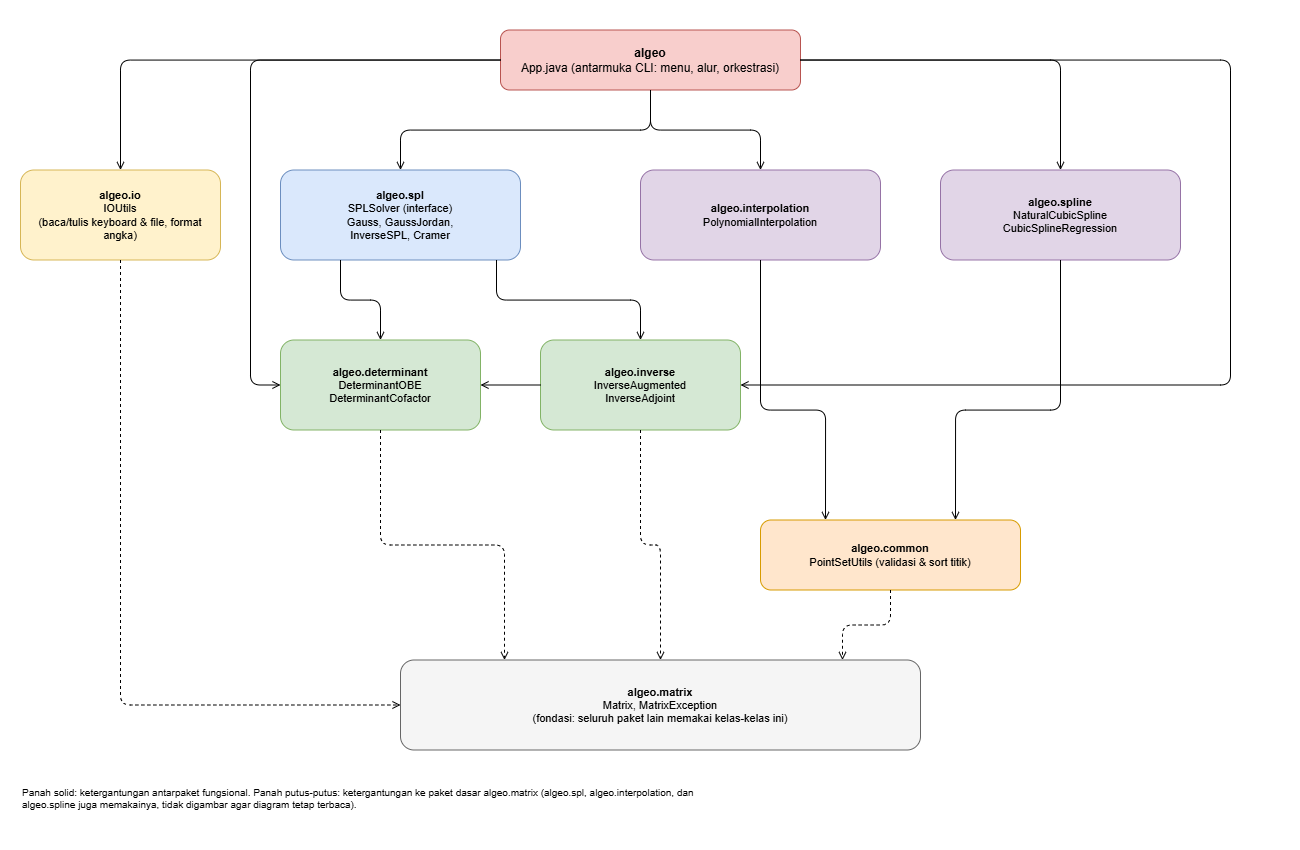
\includegraphics[width=0.70\textwidth]{diagram-arsitektur.png}
    \caption{Arsitektur pustaka dan ketergantungan antarpaket}
    \label{fig:arsitektur}
\end{figure}

\subsection{Prinsip Perancangan}

\begin{itemize}
  \item \textbf{Penggunaan ulang kode.} \texttt{DeterminantOBE} dipakai oleh
    \texttt{Cramer}, \texttt{InverseSPL}, dan \texttt{InverseAdjoint};
    \texttt{InverseAugmented} dipakai oleh \texttt{InverseSPL}; \newline
    \texttt{PointSetUtils} dipakai bersama oleh interpolasi polinomial, spline
    natural, dan regresi spline.
  \item \textbf{Pola \textit{Strategy}.} Keempat metode SPL mengimplementasikan
    \texttt{SPLSolver}, sehingga \texttt{App} cukup memilih objek yang sesuai
    lalu memanggil \texttt{isApplicable} dan \texttt{solve}.
  \item \textbf{Pemisahan logika dan tampilan.} Kelas algoritma tidak
    mencetak ke layar; hasil dikembalikan sebagai \texttt{double}, objek
    kurva, atau \texttt{String} langkah penyelesaian, dan \texttt{App}-lah yang
    mencetak serta menyimpannya. Karena itu pustaka dapat dipakai ulang oleh
    antarmuka lain.
  \item \textbf{Penanganan kesalahan terpusat.} Seluruh pelanggaran domain
    dilaporkan sebagai \texttt{MatrixException} dan ditangkap di
    \texttt{App.main}, sehingga program tidak berhenti akibat masukan salah.
  \item \textbf{Ketahanan data.} Metode \texttt{solve} bekerja pada salinan
    matriks (\texttt{copy()}) agar masukan pengguna tidak berubah, dan
    metode \textit{getter} array mengembalikan hasil \texttt{clone()}.
\end{itemize}

\subsection{Struktur Direktori Proyek}

Proyek mengikuti tata letak standar Maven; nama paket Java sama dengan
struktur foldernya.

\begin{lstlisting}
algeo26-tb1-Padang/
|-- .vscode
    |-- settings.json
|-- bin
    |-- .gitkeep/
    |-- matrix-calculator-1.0-SNAPSHOT.jar
|-- docs
    |-- .gitkeep/
|-- src/main/
    |-- java/algeo/
    |   |-- App.java
    |   |-- GuiApp.java
    |   |-- common/
    |   |   `-- PointSetUtils.java
    |   |-- determinant/
    |   |   |-- DeterminantCofactor.java
    |   |   `-- DeterminantOBE.java
    |   |-- interpolation/
    |   |   `--PolynomialInterpolation.java
    |   |-- inverse/
    |   |   |-- InverseAdjoint.java
    |   |   `-- InverseAugmented.java
    |   |-- io/
    |   |   `-- IOUtils.java
    |   |-- matrix/
    |   |   |-- Matrix.java
    |   |   `-- MatrixException.java
    |   |-- spl/
    |   |   |-- SPLSolver.java
    |   |   |-- Gauss.java
    |   |   |-- GaussJordan.java
    |   |   |-- InverseSPL.java
    |   |   `-- Cramer.java
    |   `-- spline/
    |       |-- NaturalCubicSpline.java
    |       `-- CubicSplineRegression.java
    `-- resources
        |-- algeo/gui/
            `-- fonts/
                |-- Poppins-Bold.ttf
                |-- Poppins-Regular.ttf
                `-- Poppins-SemiBold.ttf
        |-- itb + stei.png
        |-- itb.png
        `-- stei.png
|-- test
|-- .gitignore
|-- README.md
`-- pom.xml
\end{lstlisting}

\section{Alur Program}

Alur program secara garis besar ditunjukkan pada Gambar~\ref{fig:alur}.

\begin{figure}[h]
  \centering
  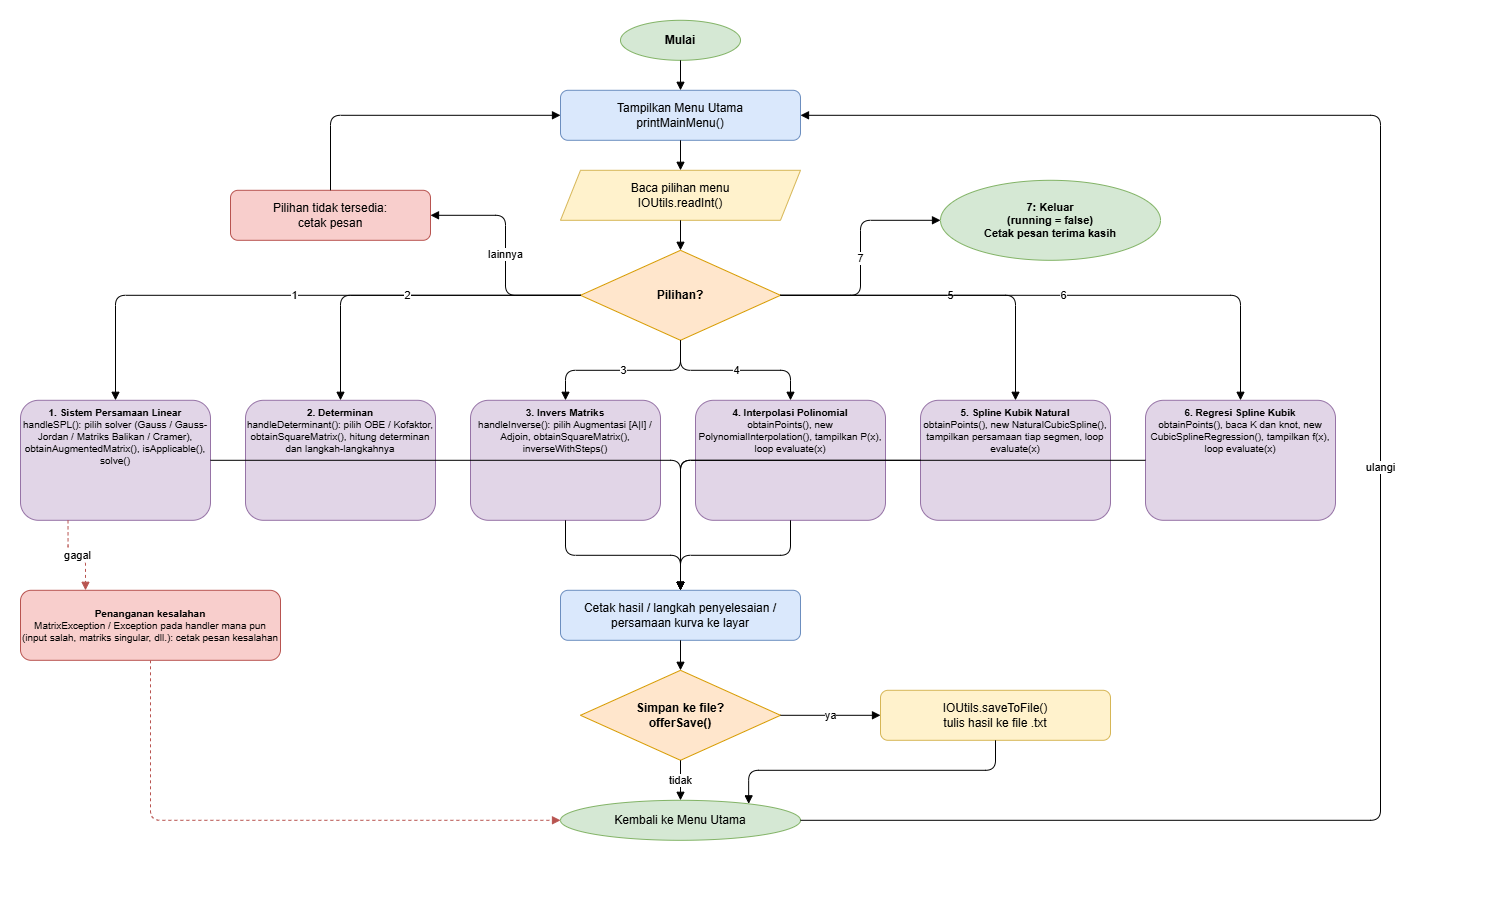
\includegraphics[width=\textwidth]{diagram-alur.png}
  \caption{Alur program secara garis besar}
  \label{fig:alur}
\end{figure}

\subsection{Alur Utama}

\begin{enumerate}
  \item Program dimulai dari \texttt{App.main}, yang membuat objek
    \texttt{Scanner} untuk membaca masukan dari keyboard.
  \item Selama \texttt{running} bernilai \texttt{true}, program menampilkan
    menu utama (\texttt{printMainMenu}) dan membaca pilihan pengguna dengan
    \texttt{IOUtils.readInt}.
  \item Pilihan diteruskan ke \texttt{handler} yang sesuai: 1 SPL,
    2 determinan, 3 invers, 4 interpolasi polinomial, 5 spline kubik natural,
    6 regresi spline kubik. Pilihan 7 mengakhiri perulangan dan program
    berhenti; angka lain menghasilkan pesan bahwa pilihan tidak tersedia.
  \item Setiap \textit{handler} meminta masukan (dari keyboard atau berkas
    \texttt{.txt}), memanggil kelas perhitungan, mencetak hasil ke layar, dan
    menawarkan penyimpanan hasil ke berkas \texttt{.txt} melalui
    \texttt{offerSave}.
  \item Bila terjadi \texttt{MatrixException} (misalnya matriks singular atau
    format berkas salah) atau \texttt{Exception} lain, pesan kesalahan
    dicetak dan program kembali ke menu utama, bukan berhenti.
  \item Setelah selesai, program kembali ke langkah 2.
\end{enumerate}

\subsection{Pemilihan Sumber Data}

Untuk semua fitur, \texttt{askInputSource} menawarkan dua sumber data:
(1) diketik langsung lewat keyboard, atau (2) dibaca dari berkas \texttt{.txt}.
Masukan manual dibatasi maksimal 11 baris dan 12 kolom untuk matriks augmented,
sedangkan berkas dibatasi 1001 baris dan 1002 kolom. Untuk data titik,
jumlah titik dibatasi maksimal 10. Berkas yang mengandung baris kosong di
tengah atau jumlah kolom yang tidak seragam ditolak dengan pesan kesalahan.

\subsection{Alur Sistem Persamaan Linear}

\begin{enumerate}
  \item Pengguna memilih metode (Gauss, Gauss-Jordan, Matriks Balikan, atau
    Kaidah Cramer); \texttt{App} membuat objek \texttt{SPLSolver} yang sesuai.
  \item Matriks augmented $[A \mid b]$ dibaca melalui
    \texttt{obtainAugmentedMatrix}.
  \item \texttt{isApplicable} diperiksa. Metode Matriks Balikan dan Cramer
    hanya berlaku bila jumlah persamaan sama dengan jumlah variabel.
  \item \texttt{solve} dijalankan dan mengembalikan \texttt{String} berisi
    langkah dan hasil.
\end{enumerate}

Rincian tiap metode:

\begin{itemize}
  \item \textbf{Gauss}: eliminasi maju dengan \textit{partial pivoting},
    normalisasi pivot menjadi 1, dan penghapusan elemen di bawah pivot.
    Baris $[0\ 0\ \cdots\ 0 \mid k]$ dengan $k \neq 0$ menandakan SPL tidak
    memiliki solusi. Bila konsisten, variabel tanpa pivot menjadi parameter
    $t_1, t_2, \dots$ dan variabel pivot dihitung dengan substitusi mundur.
  \item \textbf{Gauss-Jordan}: sama seperti Gauss, dilanjutkan eliminasi mundur
    agar elemen di atas pivot juga nol; solusi dibaca langsung dari matriks
    eselon baris tereduksi.
  \item \textbf{Matriks Balikan}: memeriksa $\det(A) \neq 0$, menghitung
    $A^{-1}$ lewat $[A \mid I]$, lalu $x = A^{-1}b$.
  \item \textbf{Kaidah Cramer}: menghitung $\det(A)$; bila bukan nol, kolom
    ke-$i$ diganti vektor $b$ untuk memperoleh $A_i$, dan
    $x_i = \det(A_i)/\det(A)$.
\end{itemize}

\subsection{Alur Determinan dan Invers}

Pengguna memilih metode, program membaca matriks persegi melalui
\texttt{obtainSquare \newline Matrix} (menolak matriks non-persegi), lalu memanggil
metode \texttt{...WithSteps} untuk mendapatkan langkah penyelesaian.
Determinan OBE mereduksi matriks menjadi segitiga atas dan mengalikan
diagonalnya; determinan kofaktor mengekspansi baris atau kolom dengan nol
terbanyak secara rekursif. Invers augmentasi mereduksi $[A \mid I]$ menjadi
$[I \mid A^{-1}]$; invers adjoin menghitung
$\frac{1}{\det(A)}\,\mathrm{adj}(A)$. Bila matriks singular, dilempar
\texttt{MatrixException} dan pengguna diberi tahu bahwa invers tidak ada.

\subsection{Alur Interpolasi dan Regresi}

\begin{enumerate}
  \item Titik data dibaca melalui \texttt{obtainPoints}. Untuk regresi, jumlah
    knot $K$ dan posisi setiap knot juga dibaca.
  \item Konstruktor kelas kurva memanggil \texttt{PointSetUtils.validateAndSort}
    (2--10 titik, terurut menaik, tanpa $x$ duplikat).
  \item Koefisien dihitung:
    \begin{itemize}
      \item \textit{Interpolasi polinomial}: menyelesaikan sistem Vandermonde
        derajat $n-1$ dengan eliminasi Gauss.
      \item \textit{Spline kubik natural}: menyelesaikan sistem tridiagonal
        untuk $c_j$ dengan $S''(x_0) = S''(x_n) = 0$, lalu menurunkan $b_j$
        dan $d_j$.
      \item \textit{Regresi spline kubik}: knot divalidasi (berada di dalam
        rentang data, tidak duplikat), matriks desain $X$ dibentuk dari basis
        $1, x, x^2, x^3, (x-\xi_j)_+^3$, lalu persamaan normal
        $(X^{\top}X)\beta = X^{\top}y$ diselesaikan dengan Gauss-Jordan.
    \end{itemize}
  \item Program mencetak rentang data dan persamaan kurva, lalu memasuki
    perulangan evaluasi: pengguna memasukkan nilai $x$, program mencetak
    nilai fungsi, dan bila $x$ di luar rentang data ditambahkan peringatan
    ekstrapolasi. Perulangan berhenti saat pengguna menekan Enter pada baris
    kosong.
  \item Hasil, persamaan kurva, dan catatan evaluasi dapat disimpan ke
    berkas \texttt{.txt}.
\end{enumerate}


\section{Build Tool dan Packaging}


\subsection{Maven sebagai Build Tool}

Proyek ini memakai Apache Maven untuk mengelola kompilasi, dependensi, dan
pembuatan berkas \texttt{.jar}. Konfigurasi proyek dituliskan pada berkas
\texttt{pom.xml} di direktori utama, dengan isi pokok sebagai berikut.

\begin{itemize}
  \item \textbf{Koordinat proyek}: \texttt{groupId} = \texttt{algeo},
    \texttt{artifactId} = \texttt{matrix-calculator}, \texttt{version} =
    \texttt{1.0-SNAPSHOT}.
  \item \textbf{Properti}: kompilator diatur ke Java 21
    (\texttt{maven.compiler.source} dan \texttt{maven. \newline compiler.target}),
    pengkodean sumber UTF-8, dan \texttt{javafx.version} = 21.0.5.
  \item \textbf{Dependensi}: \texttt{javafx-controls} dan \texttt{javafx-fxml}
    dari \texttt{org.openjfx}, yang diunduh otomatis dari Maven Central.
    Versi pada properti \texttt{javafx.version} dipakai bersama oleh keduanya.
  \item \textbf{Plugin}: \texttt{exec-maven-plugin} (3.1.0) dengan
    \texttt{mainClass} = \texttt{algeo.App} untuk menjalankan versi CLI, dan
    \texttt{javafx-maven-plugin} (0.0.8) untuk menjalankan versi GUI.
\end{itemize}

Maven bekerja dengan \textit{build lifecycle}. Fase yang paling sering dipakai
adalah \texttt{compile} (mengompilasi kode di \texttt{src/main/java} ke
\texttt{target/classes}), \texttt{test}, \texttt{package} (membuat \texttt{.jar}
di folder \texttt{target}), dan \texttt{install} (menyalin artefak ke repositori
lokal). Menjalankan suatu fase otomatis menjalankan fase-fase sebelumnya.

\subsection{Perintah Build dan Menjalankan Program}

\begin{verbatim}
# membersihkan hasil build lama dan mengompilasi
mvn clean compile

# menjalankan program CLI langsung dari Maven (kelas utama 
algeo.App)
mvn exec:java

# membuat berkas .jar
mvn clean package
\end{verbatim}

Perintah \texttt{mvn clean package} menghasilkan berkas \texttt{target/matrix-calculator- \newline 1.0-SNAPSHOT.jar}. Nama berkas ini berasal dari \texttt{artifactId} dan \texttt{version} yang didefinisikan pada \texttt{pom.xml}.

Perintah \texttt{mvn clean package} menghasilkan berkas
\texttt{target/matrix-calculator- \newline 1.0-SNAPSHOT.jar}. Nama berkas berasal dari
\texttt{artifactId} dan \texttt{version} pada \texttt{pom.xml}.

\subsection{Pembuatan Berkas .jar yang Dapat Dieksekusi}

Secara bawaan, \textit{jar} yang dibuat Maven belum memiliki atribut \texttt{Main-Class} pada \texttt{MANIFEST. \newline MF}, sehingga tidak dapat dijalankan dengan \texttt{java -jar}. Agar dapat dieksekusi langsung, ditambahkan \texttt{maven-jar-plugin} pada bagian \texttt{<build><plugins>} di \texttt{pom.xml}:

\begin{verbatim}
<plugin>
    <groupId>org.apache.maven.plugins</groupId>
    <artifactId>maven-jar-plugin</artifactId>
    <version>3.4.1</version>
    <configuration>
        <archive>
            <manifest>
                <mainClass>algeo.App</mainClass>
            </manifest>
        </archive>
    </configuration>
</plugin>
\end{verbatim}

Setelah konfigurasi \texttt{pom.xml} diperbarui, jalankan perintah \texttt{mvn clean package}. Perintah ini akan menghapus hasil build sebelumnya, mengompilasi kode, dan mengemas proyek. Hasil build akan tersimpan di dalam direktori \texttt{target/}. Berkas \textit{jar} tersebut kemudian dapat dijalankan secara langsung dengan perintah:

\begin{verbatim}
java -jar target/matrix-calculator-1.0-SNAPSHOT.jar
\end{verbatim}

Versi CLI (\texttt{algeo.App}) hanya memakai pustaka standar Java sehingga \textit{jar} tersebut dapat berjalan tanpa perlu menyertakan JavaFX. Berkas \textit{jar} ini dapat dijalankan pada komputer mana pun yang telah memasang JDK atau JRE versi 21 atau lebih baru. 

Untuk menjalankan versi antarmuka grafis (GUI) berbasis JavaFX, pengguna dapat menggunakan perintah \texttt{mvn javafx:run}. Jika kelak diperlukan \textit{jar} yang membundel seluruh dependensi eksternal (termasuk JavaFX), dapat digunakan \texttt{maven-shade-plugin}.

% BAB 4: EKSPERIMEN
\chapter{Eksperimen}

\section{Kasus Uji 4.1: Determinan Matriks}

\subsection{Kasus Uji 4.1.1: Matriks $A$ Berukuran $4 \times 4$}

\textbf{Matriks Masukan:}
\[
A =
\begin{bmatrix}
0 & 2 & -1 & 3 \\
4 & 1 & 2 & -2 \\
-2 & 3 & 0 & 1 \\
1 & -1 & 5 & 2
\end{bmatrix}
\]

\textbf{Hasil Eksekusi Program:}

\begin{figure}[H]
    \centering
    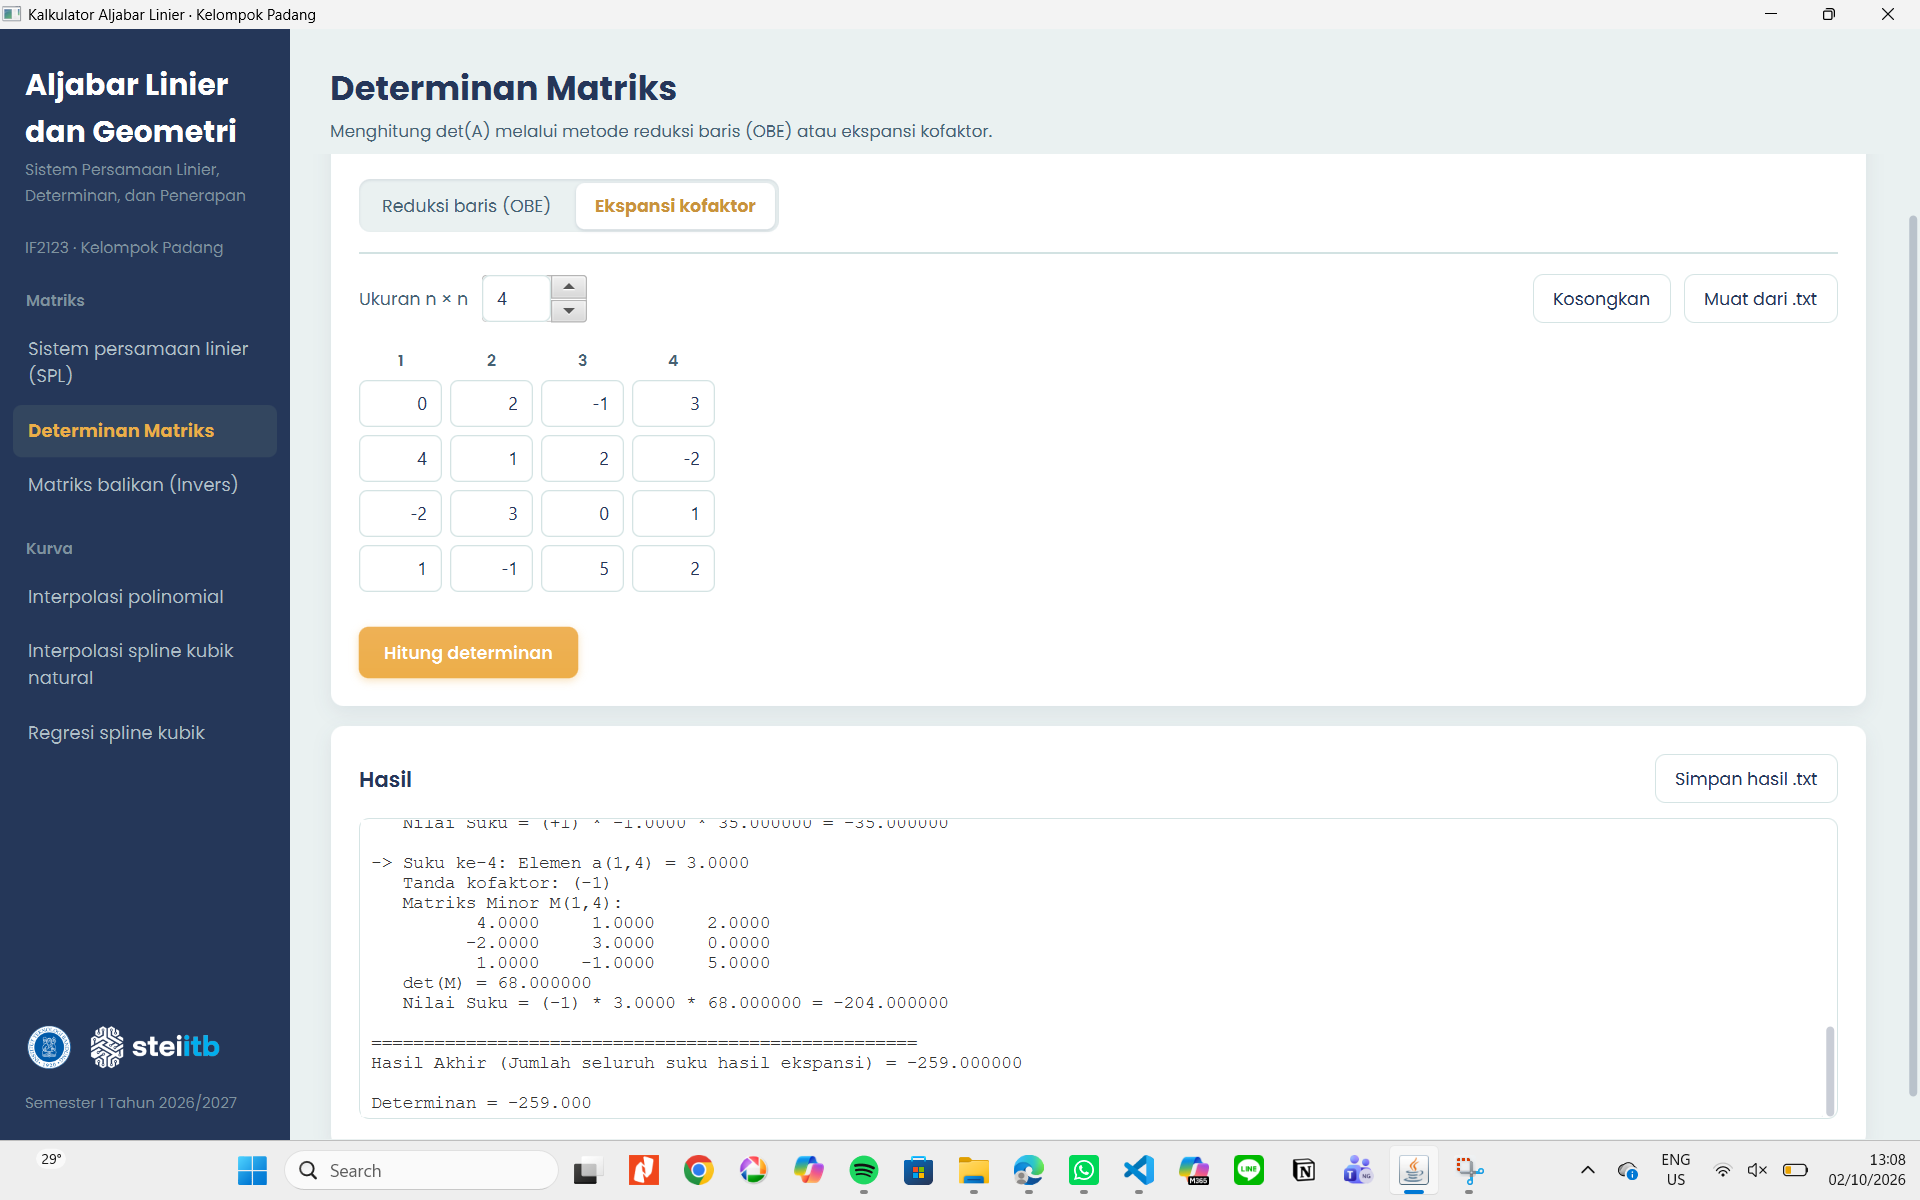
\includegraphics[width=0.7\textwidth, height=8.5cm, keepaspectratio]{uji1_det44_kofaktor.png}
    \caption{Determinan dengan Metode Ekspansi Kofaktor}
    \label{fig:det44_kofaktor}
\end{figure}

\begin{figure}[H]
    \centering
    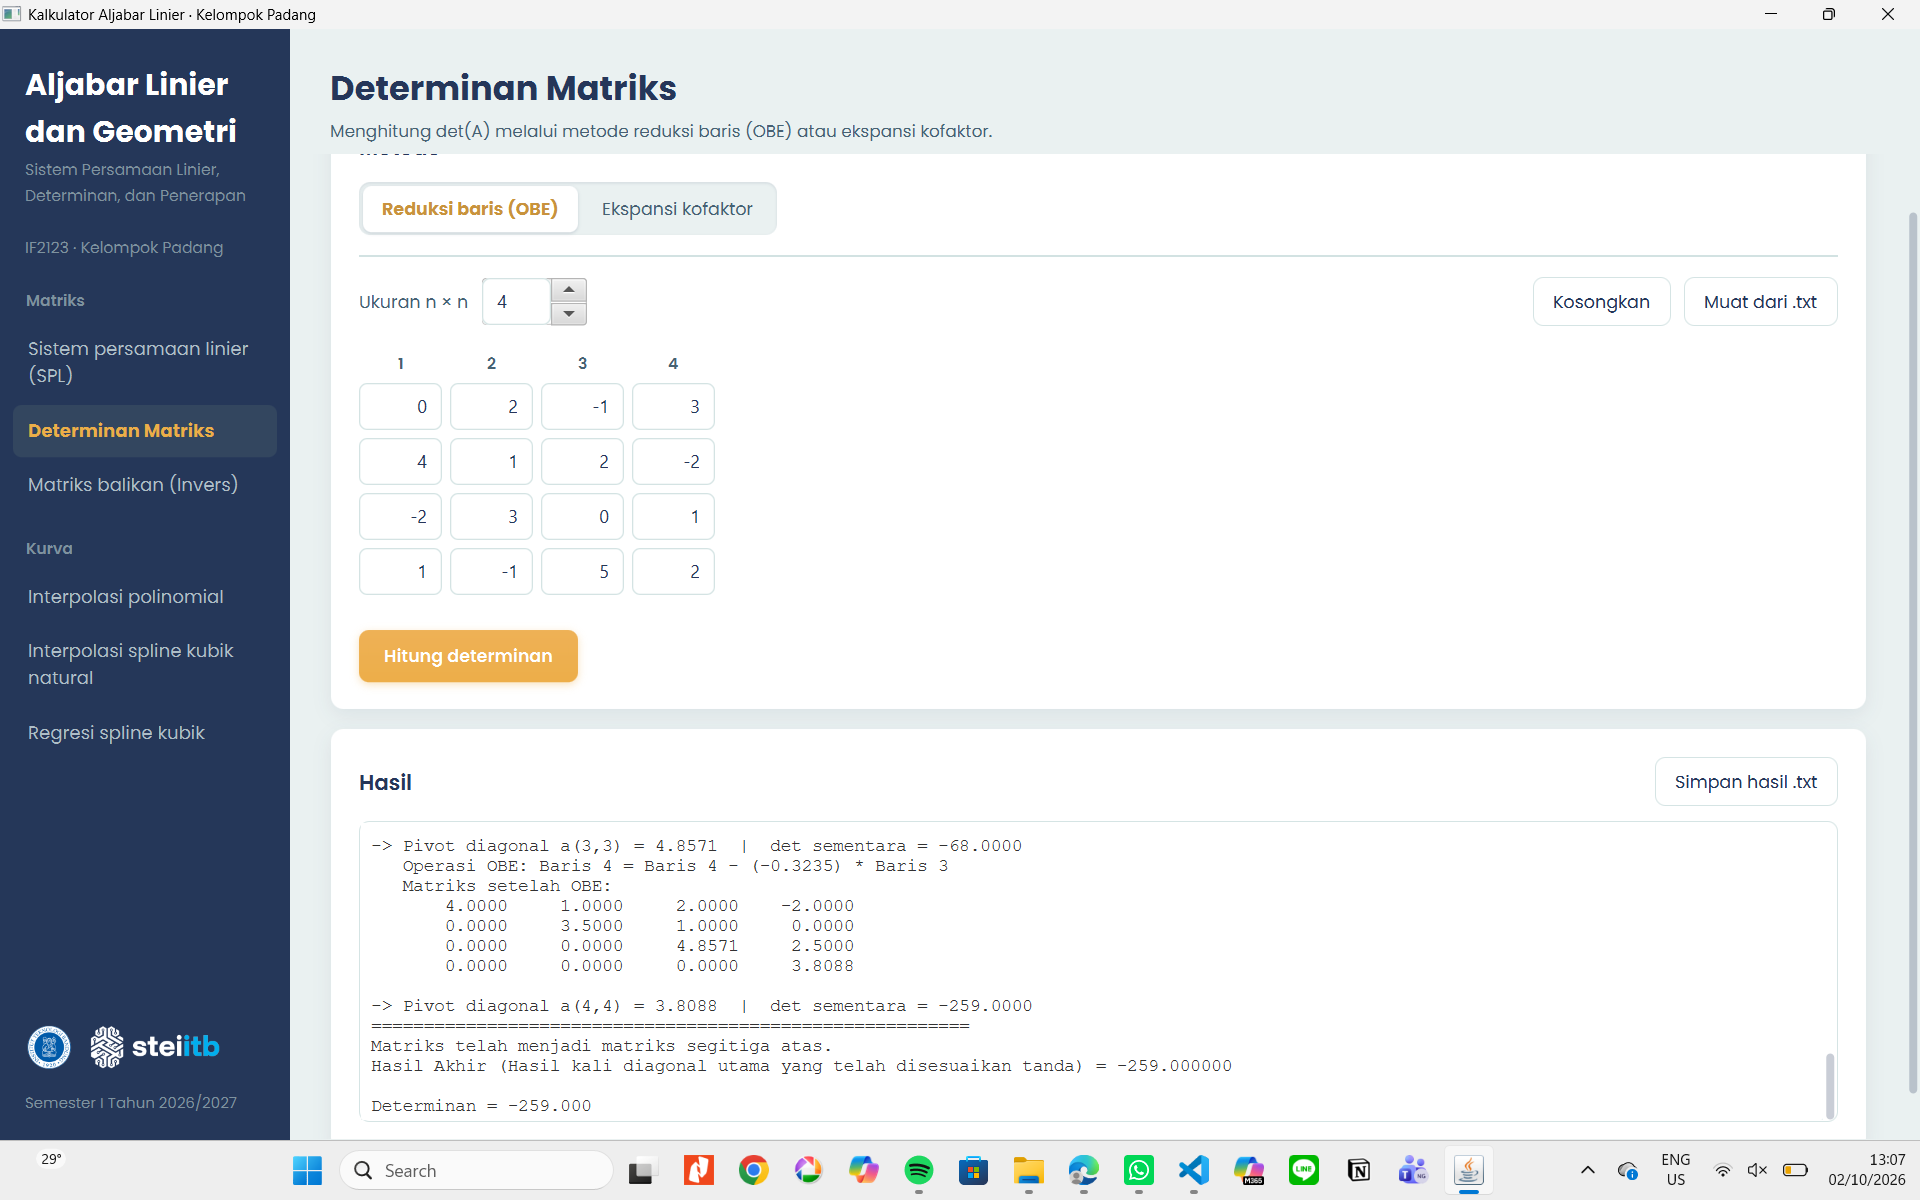
\includegraphics[width=0.7\textwidth, height=8.5cm, keepaspectratio]{uji1_det44_obe.png}
    \caption{Determinan dengan Metode Reduksi Baris (OBE)}
    \label{fig:det44_obe}
\end{figure}

\textbf{Analisis:}

Metode Reduksi Baris (OBE) dan Ekspansi Kofaktor menghasilkan nilai determinan yang sama, yaitu $\det(A)$. Penggunaan \textit{partial pivoting} pada Reduksi Baris membantu menjaga stabilitas numerik ketika terjadi pertukaran baris.


\subsection{Kasus Uji 4.1.2: Matriks $A$ Berukuran $5 \times 5$}

\textbf{Matriks Masukan:}
\[
A =
\begin{bmatrix}
2 & -1 & 3 & 0 & 4 \\
1 & 2 & -2 & 5 & -1 \\
3 & 1 & 1 & 2 & 0 \\
0 & 4 & -1 & 3 & 2 \\
5 & 0 & 4 & 2 & 4
\end{bmatrix}
\]

\textbf{Hasil Eksekusi Program:}

\begin{figure}[H]
    \centering
    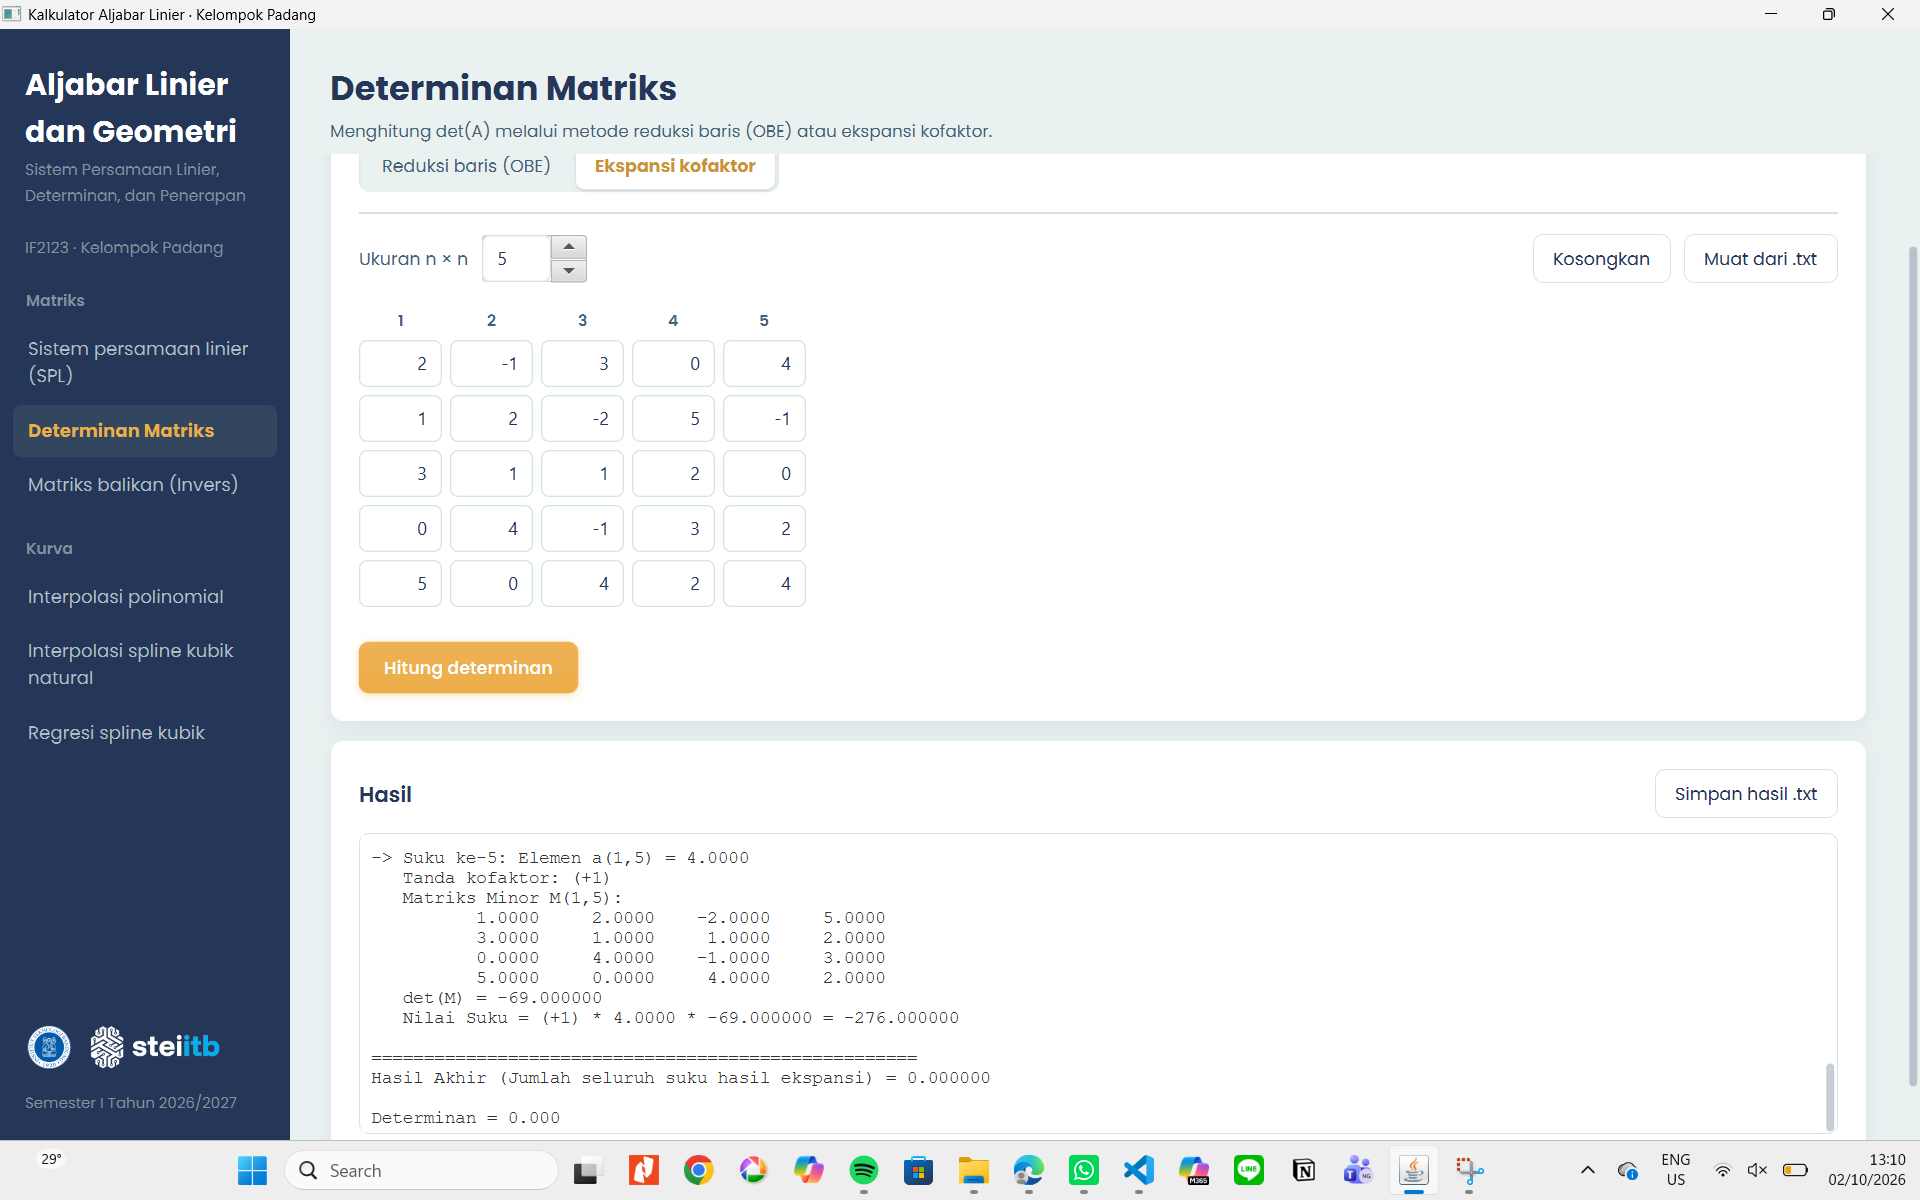
\includegraphics[width=0.7\textwidth, height=8.5cm, keepaspectratio]{uji2_det55_kofaktor.png}
    \caption{Determinan dengan Metode Ekspansi Kofaktor}
    \label{fig:det55_kofaktor}
\end{figure}

\begin{figure}[H]
    \centering
    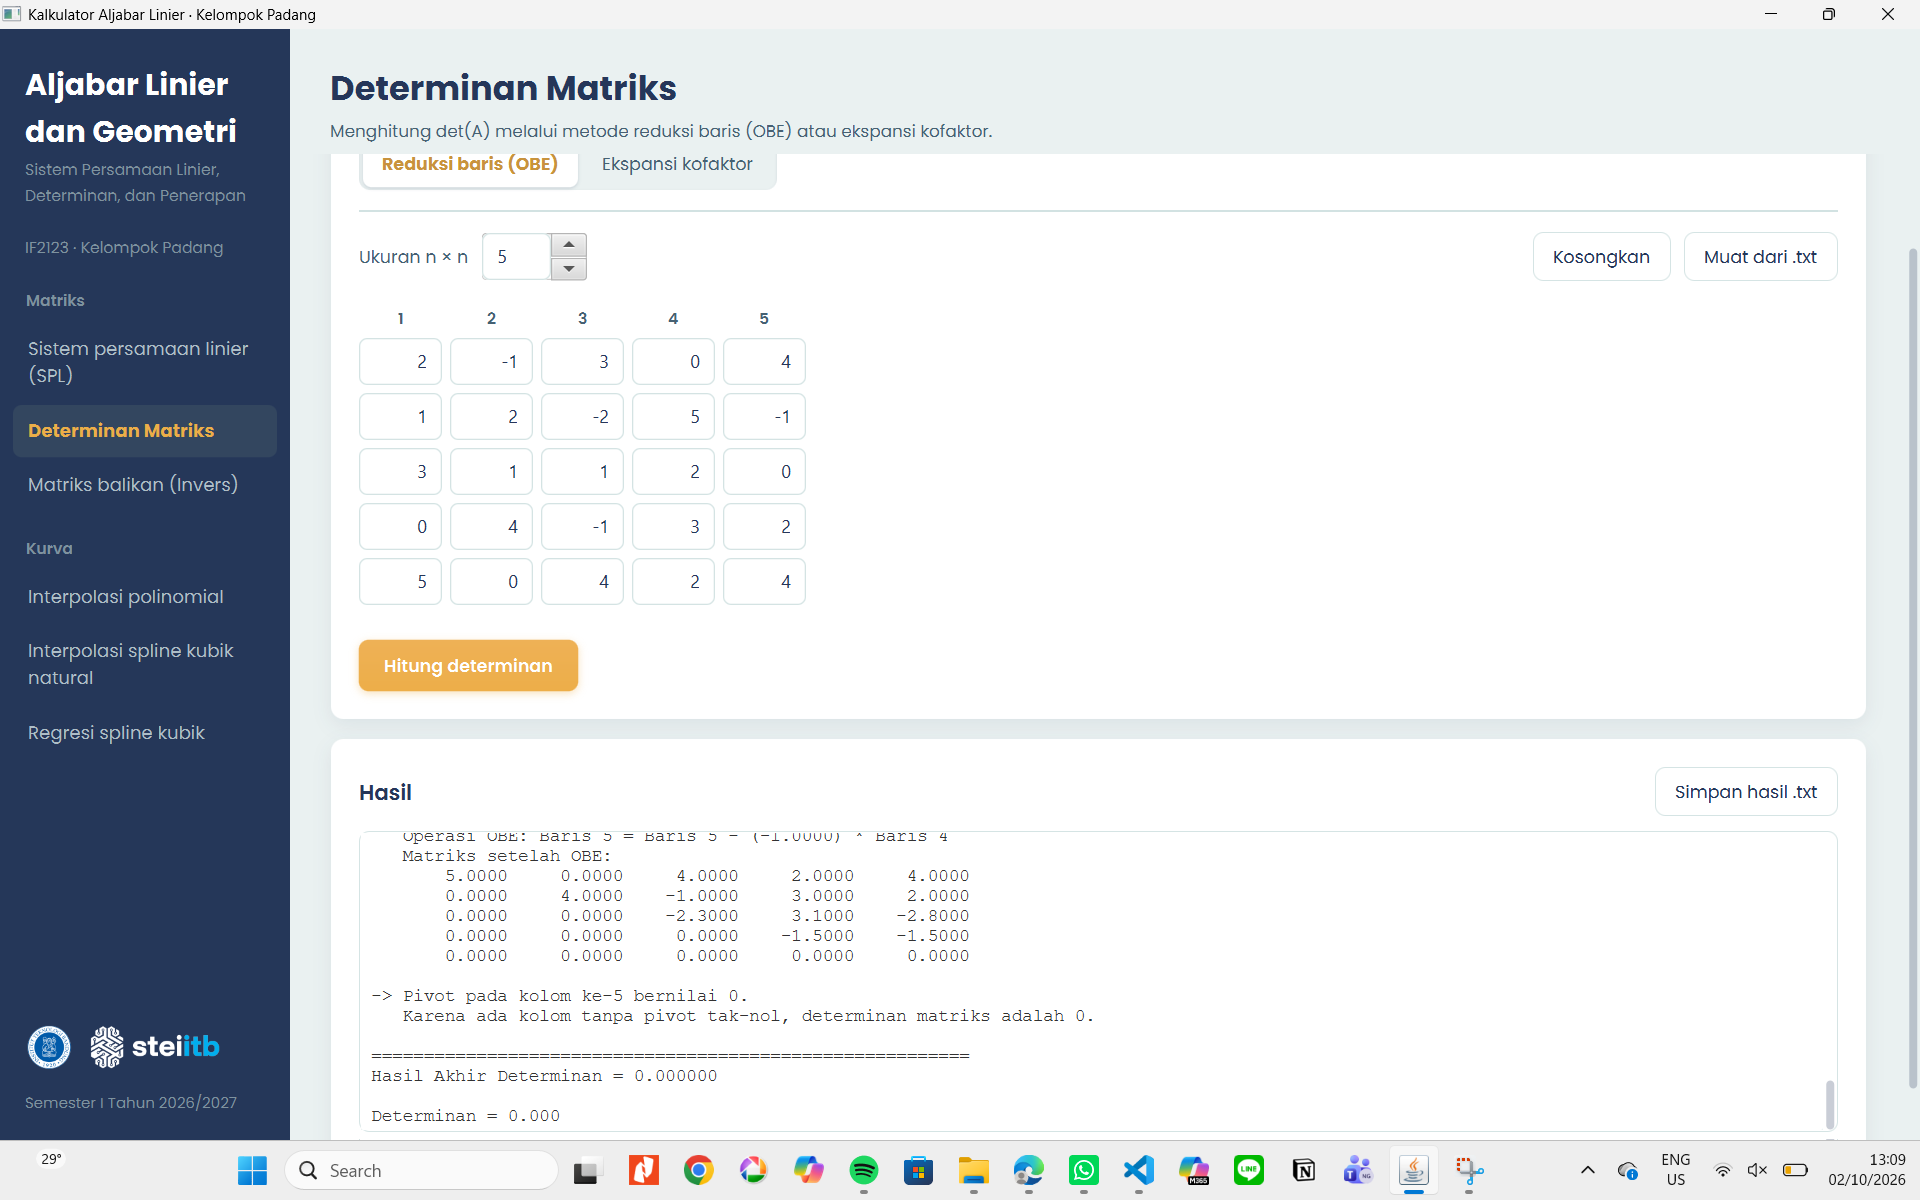
\includegraphics[width=0.7\textwidth, height=8.5cm, keepaspectratio]{uji2_det55_obe.png}
    \caption{Determinan dengan Metode Reduksi Baris (OBE)}
    \label{fig:det55_obe}
\end{figure}

\textbf{Analisis:}

Metode Reduksi Baris (OBE) dan Ekspansi Kofaktor menghasilkan nilai determinan yang sama, yaitu $\det(A)$. Pada matriks berukuran $5 \times 5$, Metode Reduksi Baris memiliki efisiensi komputasi yang lebih baik dibandingkan Ekspansi Kofaktor karena kompleksitas algoritmanya yang lebih rendah.

\subsection{Kasus Uji 4.1.3: Matriks $A$ Berukuran $4 \times 4$}

\textbf{Matriks Masukan:}
\[
A =
\begin{bmatrix}
0.5 & 1 & 0 & 0.5 \\
0.5 & 1.25 & 0.25 & 0.5 \\
-0.1 & -0.4 & 0.2 & -0.3 \\
0.6 & 1.25 & 0.45 & 0.6
\end{bmatrix}
\]

\textbf{Hasil Eksekusi Program:}

\begin{figure}[H]
    \centering
    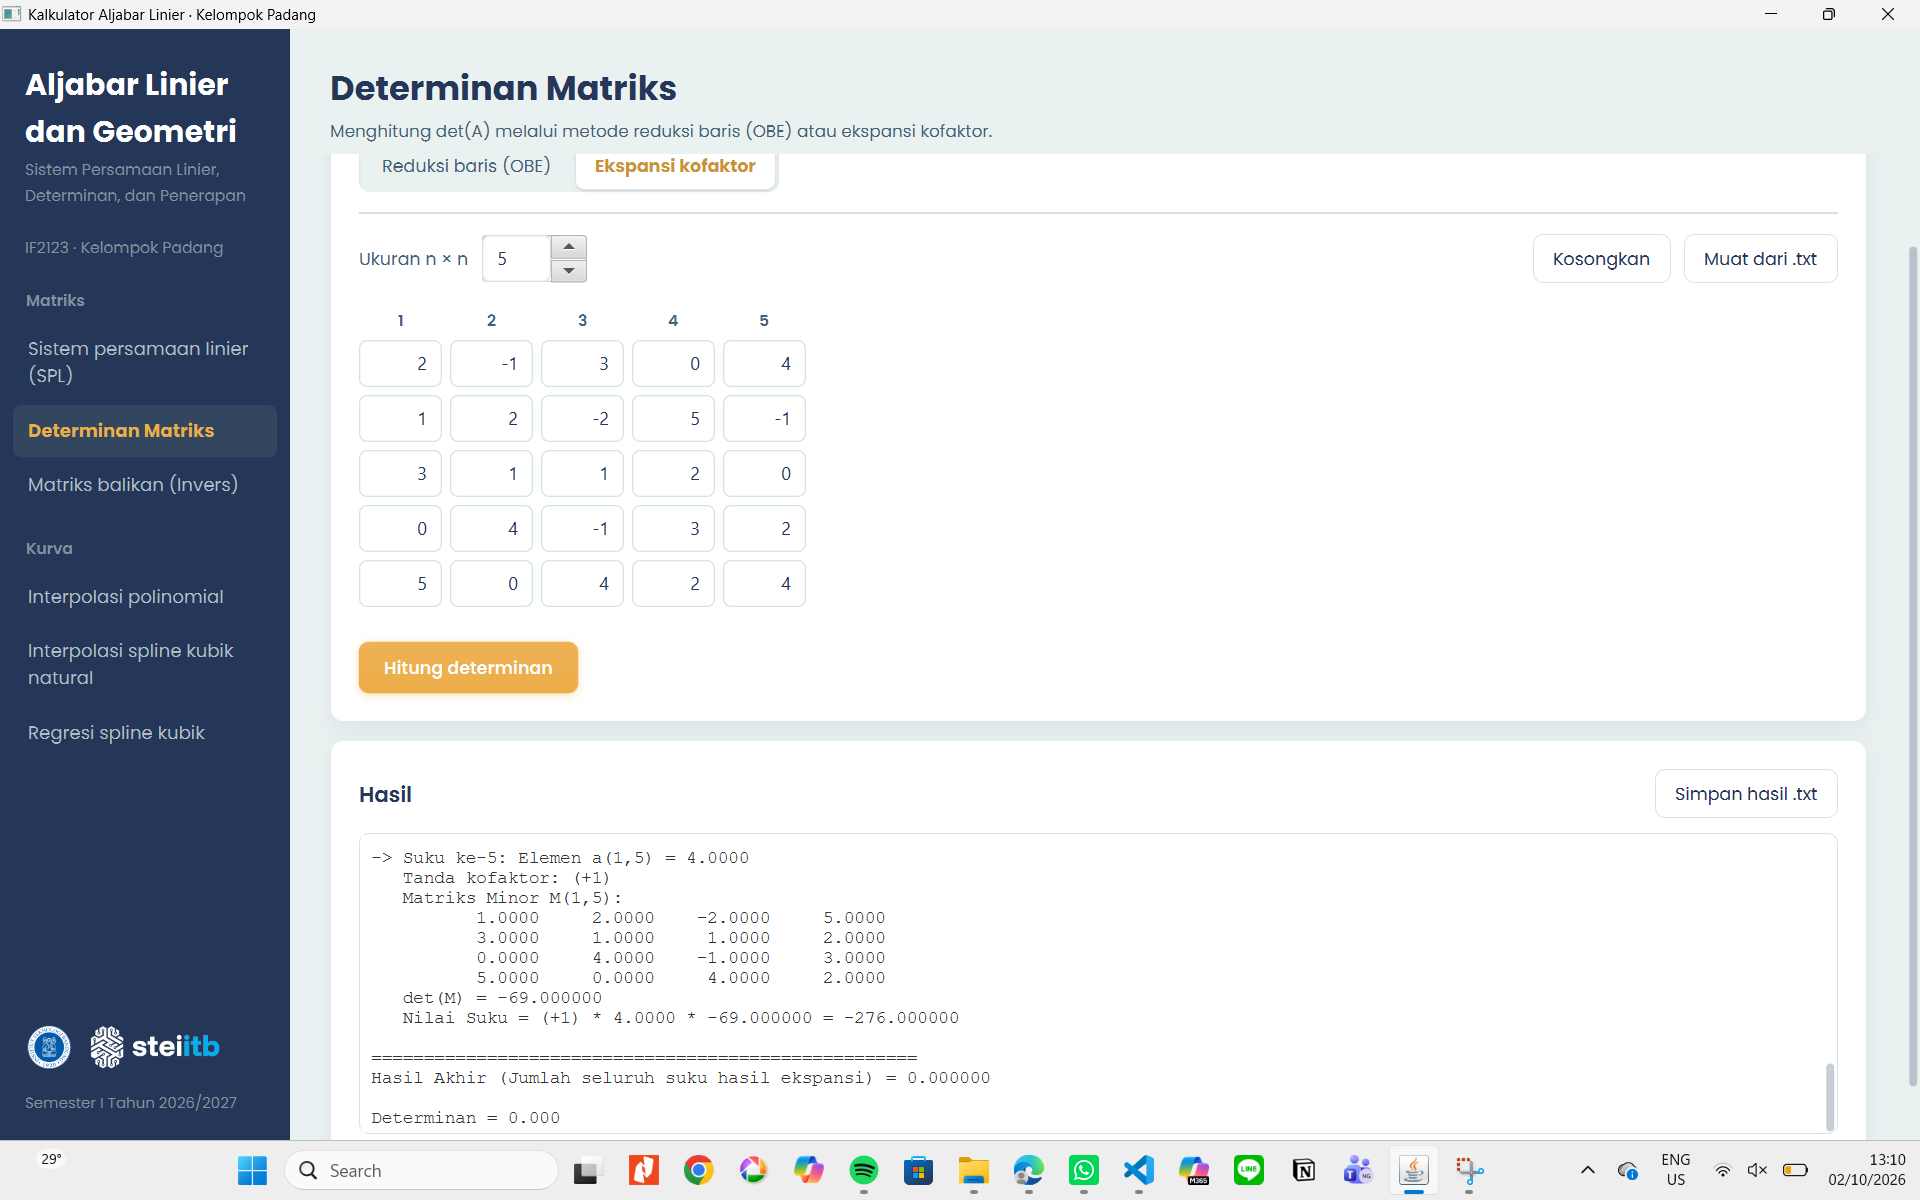
\includegraphics[width=0.7\textwidth, height=8.5cm, keepaspectratio]{uji2_det55_kofaktor.png}
    \caption{Determinan dengan Metode Ekspansi Kofaktor}
    \label{fig:det55_kofaktor}
\end{figure}

\begin{figure}[H]
    \centering
    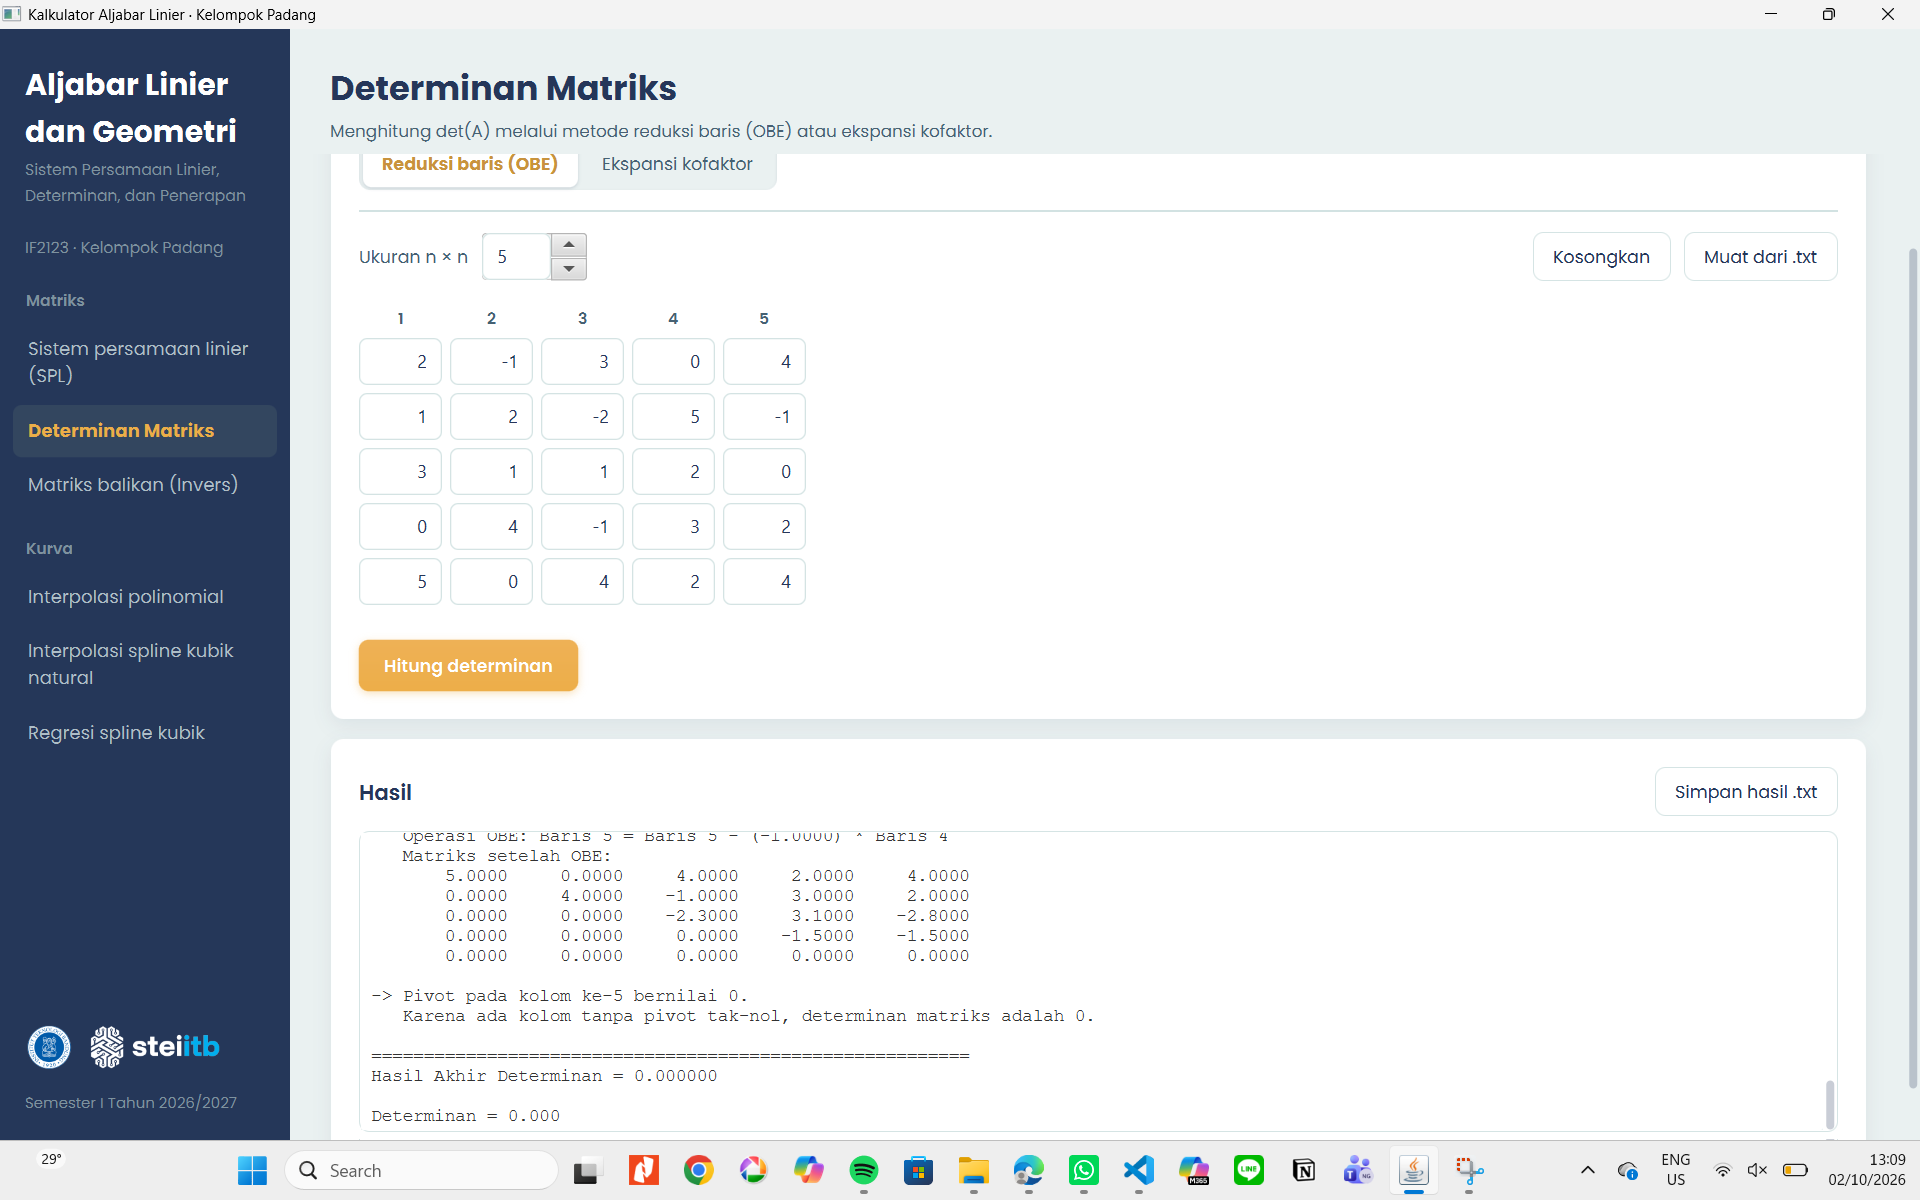
\includegraphics[width=0.7\textwidth, height=8.5cm, keepaspectratio]{uji2_det55_obe.png}
    \caption{Determinan dengan Metode Reduksi Baris (OBE)}
    \label{fig:det55_obe}
\end{figure}

\textbf{Analisis:}

Metode Reduksi Baris (OBE) dan Ekspansi Kofaktor menghasilkan nilai determinan yang sama, yaitu $\det(A)$. Pengujian pada matriks berorde $4 \times 4$ dengan nilai elemen berupa bilangan desimal menunjukkan bahwa kedua algoritma dapat menangani kalkulasi dengan presisi \textit{floating-point} secara akurat.

\section{Kasus Uji 4.2: Invers Matriks}

\subsection{Kasus Uji 4.2.1: Matriks $A$ Berukuran $4 \times 4$}

\textbf{Matriks Masukan:}
\[
A =
\begin{bmatrix}
0 & 1 & 2 & -1 \\
1 & 0 & 1 & 2 \\
2 & 1 & 0 & 1 \\
-1 & 2 & 1 & 0
\end{bmatrix}
\]

\textbf{Hasil Eksekusi Program:}

\begin{figure}[H]
    \centering
    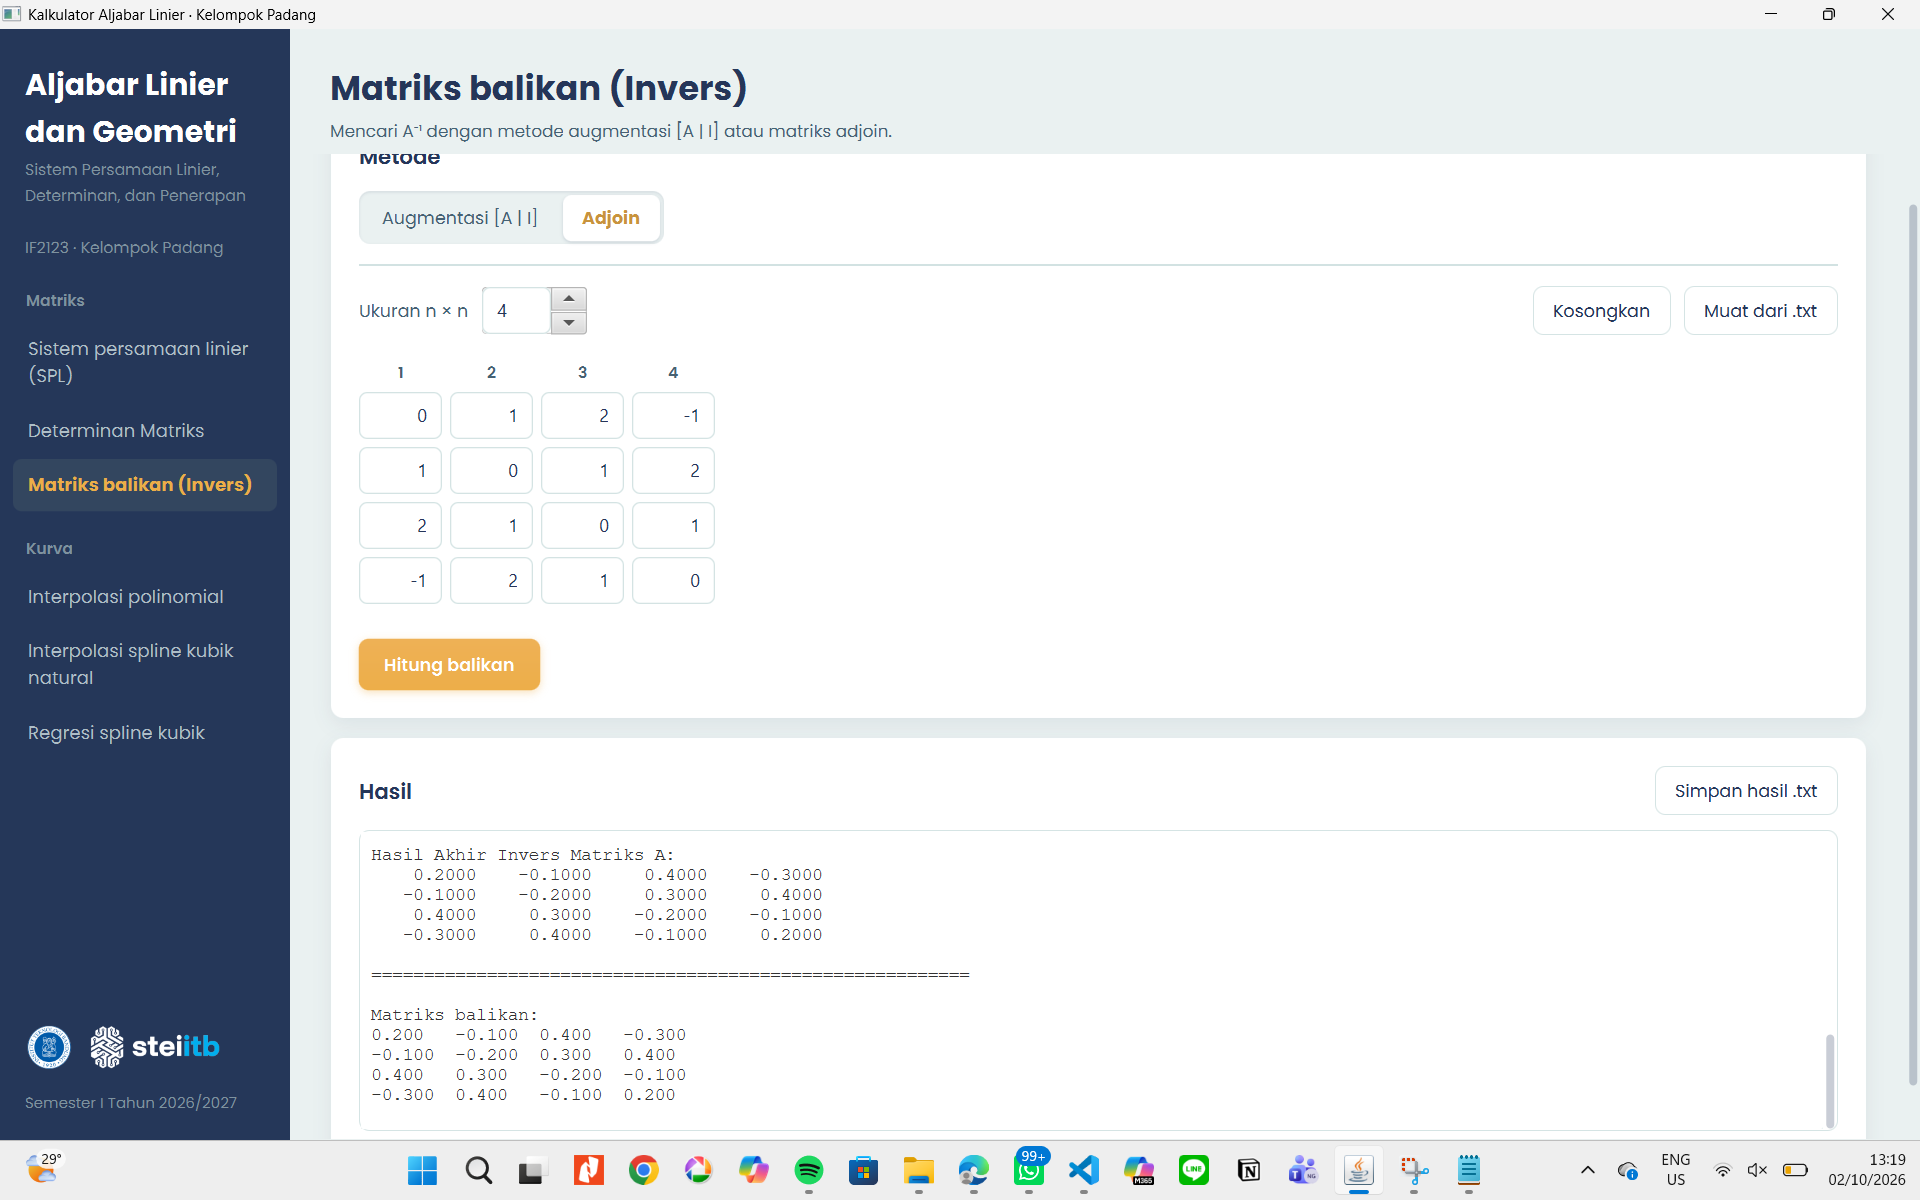
\includegraphics[width=0.7\textwidth, height=8.5cm, keepaspectratio]{uji5_inverse1_adjoin.png}
    \caption{Invers Matriks dengan Metode Adjoin}
    \label{fig:inverse1_adjoin}
\end{figure}

\begin{figure}[H]
    \centering
    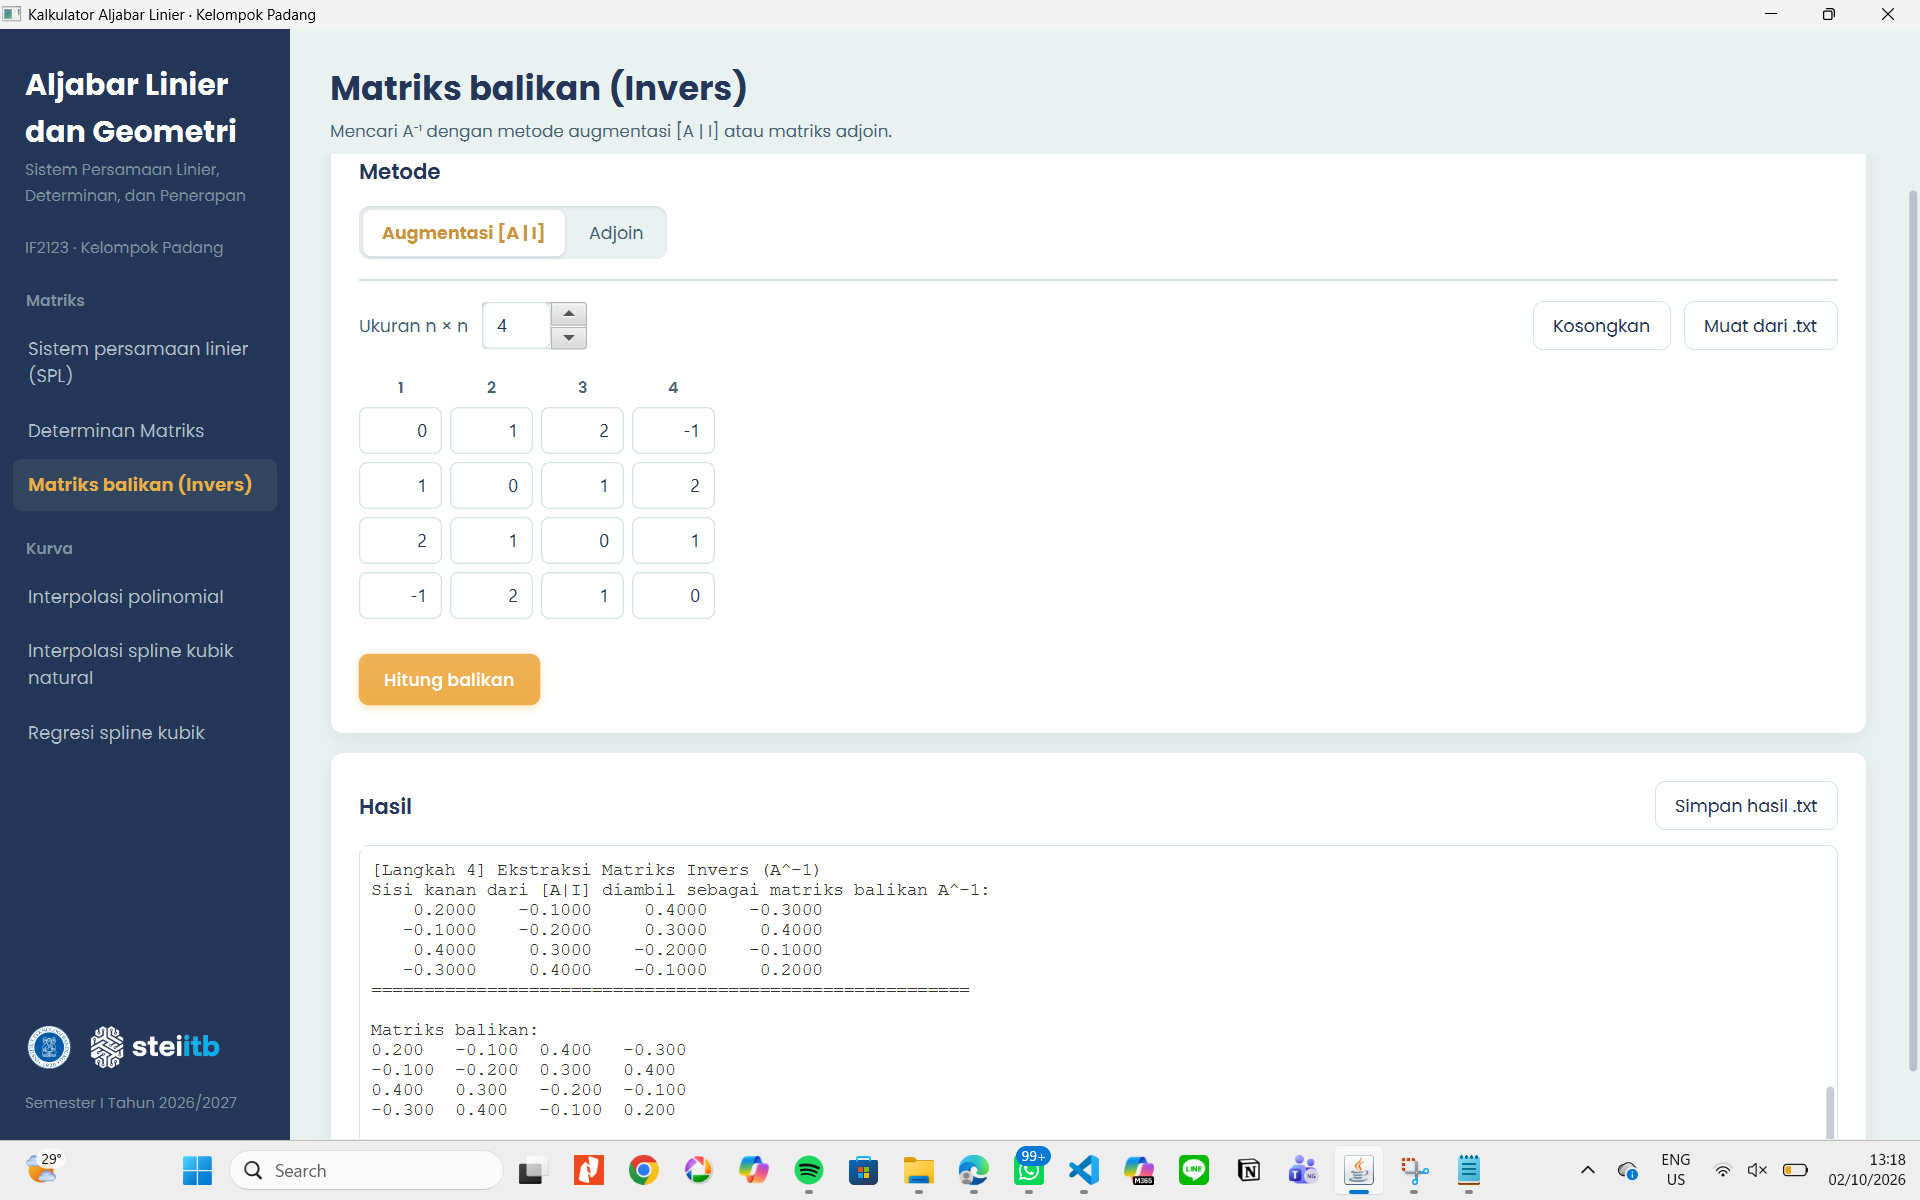
\includegraphics[width=0.7\textwidth, height=8.5cm, keepaspectratio]{uji5_inverse1_augmentasi.png}
    \caption{Invers Matriks dengan Metode Augmentasi (OBE)}
    \label{fig:inverse1_augmentasi}
\end{figure}

\textbf{Analisis:}

Kedua metode menghasilkan matriks invers yang identik. Penggunaan Metode Augmentasi (OBE) lebih efisien secara komputasi dibandingkan Metode Adjoin, terutama karena Metode Adjoin memerlukan perhitungan kofaktor dan determinan dari banyak submatriks.

\subsection{Kasus Uji 4.2.2: Matriks $A$ Berukuran $5 \times 5$}

\textbf{Matriks Masukan:}
\[
A =
\begin{bmatrix}
1 & 2 & 0 & -1 & 3 \\
2 & -1 & 4 & 0 & 1 \\
0 & 3 & 1 & 2 & -2 \\
4 & 0 & 5 & 1 & 2 \\
3 & 1 & 4 & -1 & 4
\end{bmatrix}
\]

\textbf{Hasil Eksekusi Program:}

\begin{figure}[H]
    \centering
    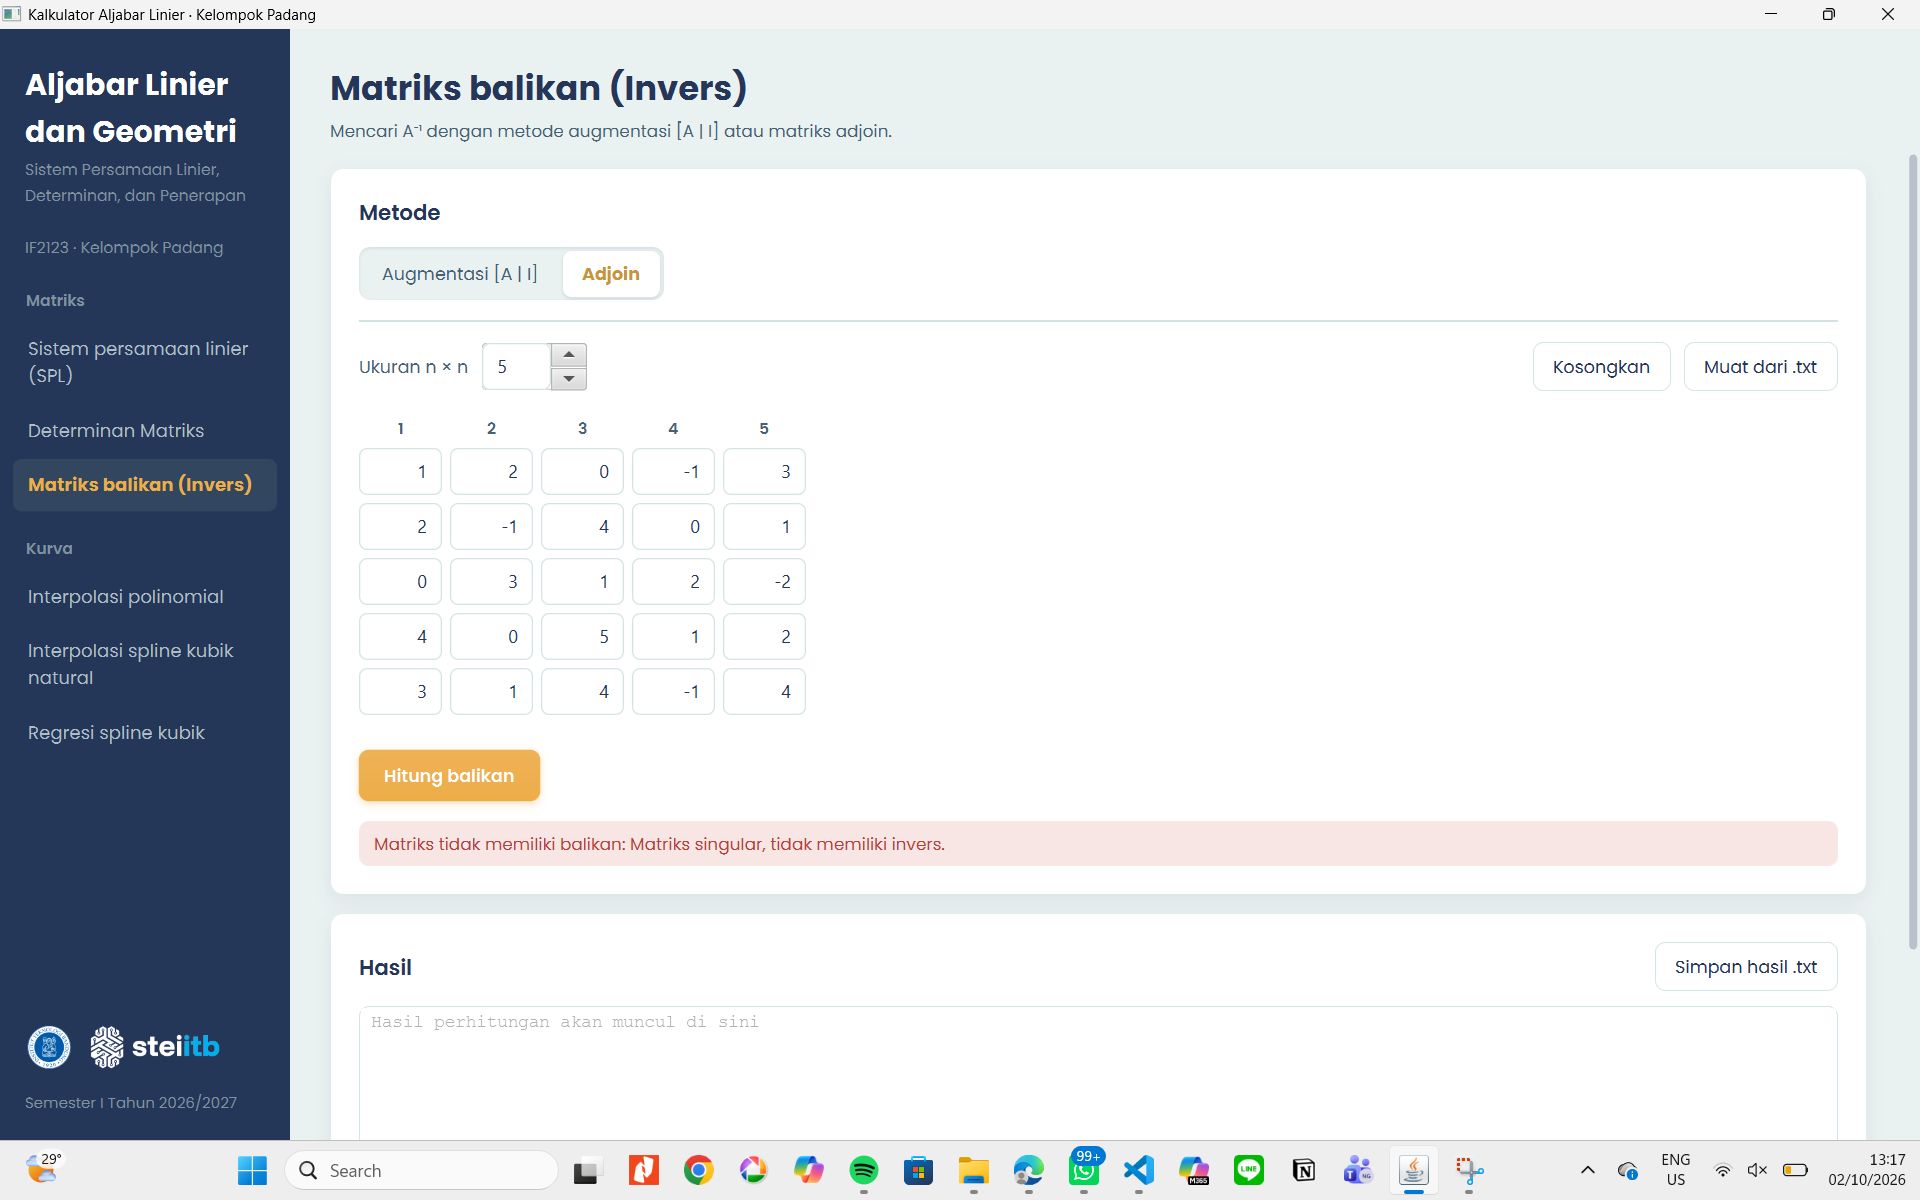
\includegraphics[width=0.7\textwidth, height=8.5cm, keepaspectratio]{uji4_inverse2_adjoin.png}
    \caption{Invers Matriks dengan Metode Adjoin}
    \label{fig:inverse2_adjoin}
\end{figure}

\begin{figure}[H]
    \centering
    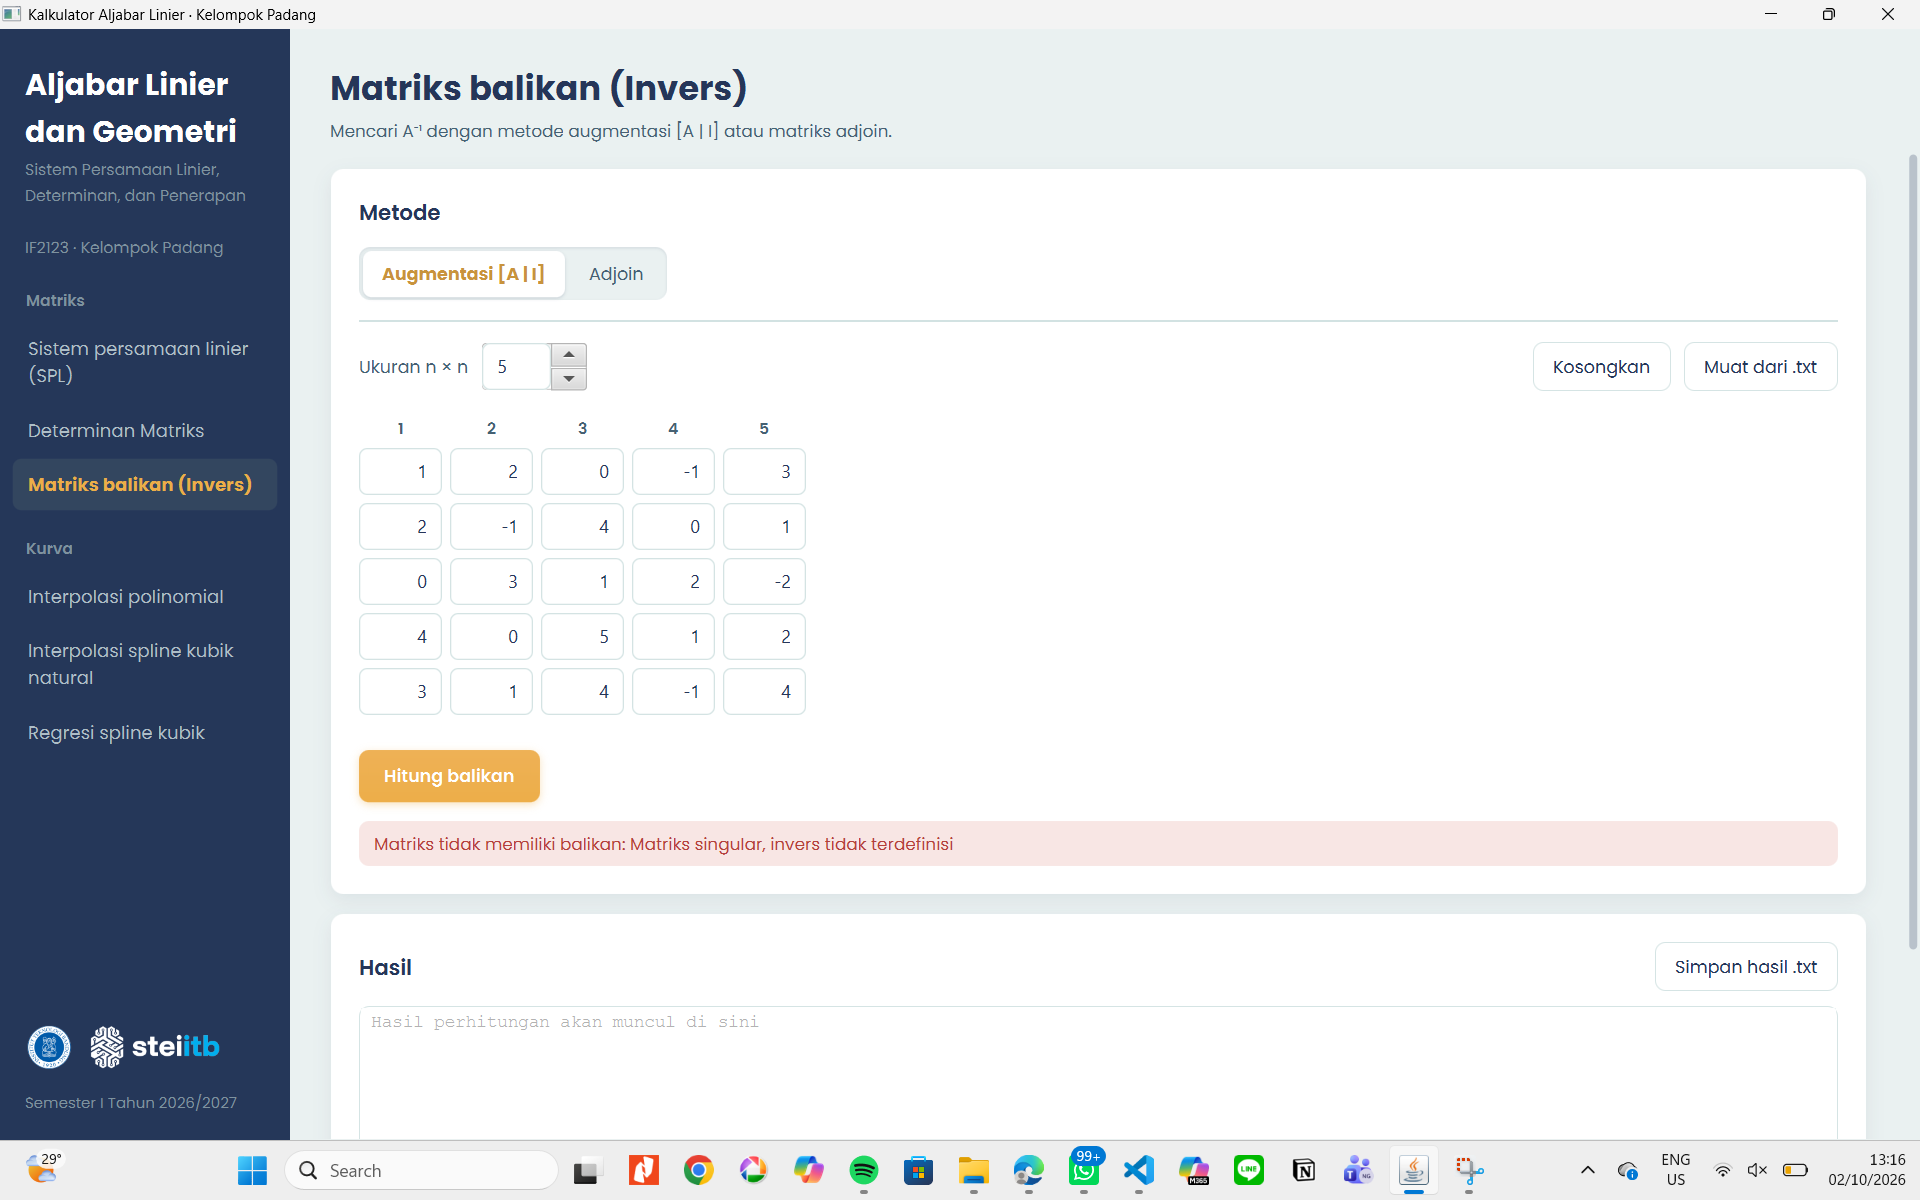
\includegraphics[width=0.7\textwidth, height=8.5cm, keepaspectratio]{uji4_inverse2_augmentasi.png}
    \caption{Invers Matriks dengan Metode Augmentasi (OBE)}
    \label{fig:inverse2_augmentasi}
\end{figure}

\textbf{Analisis:}

Metode Augmentasi dan Adjoin berhasil mendapatkan matriks invers yang sama untuk ukuran $5 \times 5$. Terlihat perbedaan performa waktu eksekusi, di mana Metode Augmentasi bekerja lebih efektif daripada Metode Adjoin pada ukuran matriks yang lebih besar.



% 5.3 Sistem Persamaan Linier (Ax = b)
\section{Kasus Uji 4.3: Sistem Persamaan Linier (\(Ax = b\))}

\subsection{Kasus Uji 4.3.1: Matriks $A$ Berukuran $4 \times 4$}
\textbf{Matriks Masukan:}
\[
A = \begin{bmatrix}
0 & 2 & -1 & 1 \\
1 & -1 & 2 & 3 \\
2 & 1 & 1 & -1 \\
-1 & 3 & 0 & 2
\end{bmatrix}, \quad
b = \begin{bmatrix}
-5 \\
15 \\
1 \\
-3
\end{bmatrix}
\]

\textbf{Hasil Eksekusi Program:}
\begin{figure}[H]
    \centering
    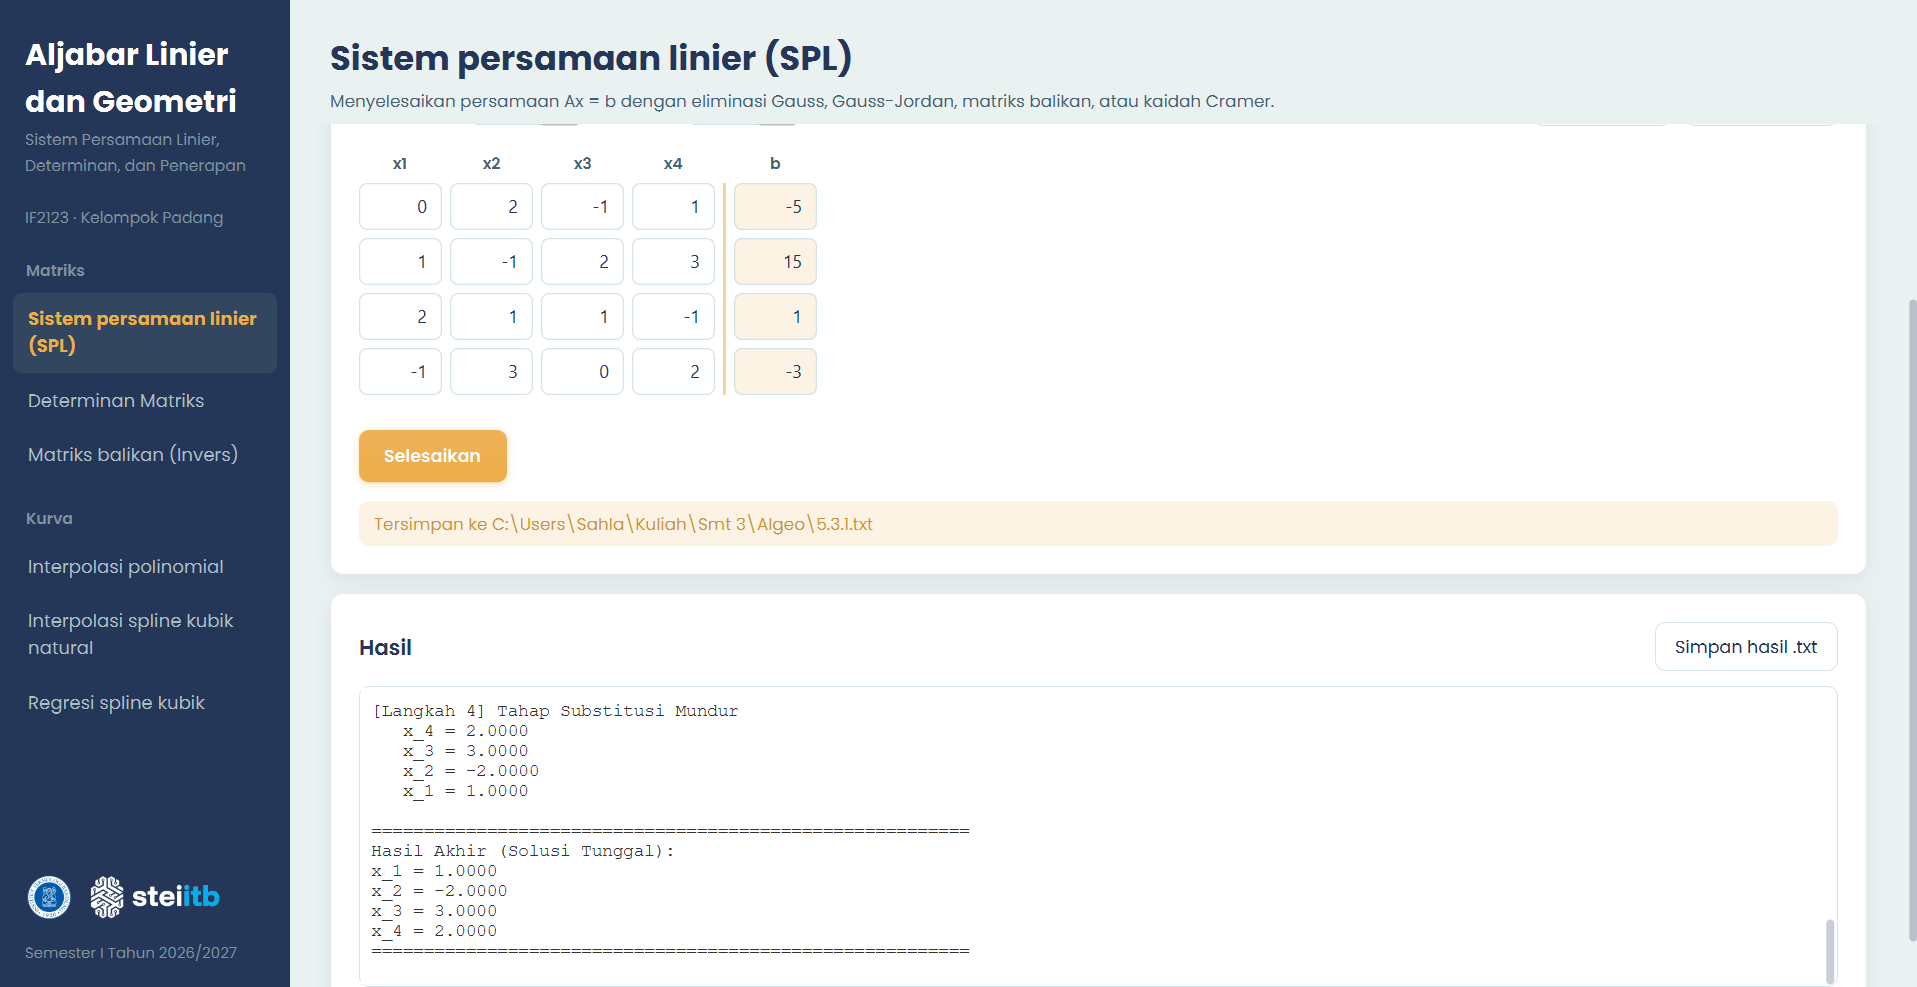
\includegraphics[width=0.8\textwidth]{5.3.1.gauss.png}
    \caption{Penyelesaian SPL dengan Metode Gauss}
\end{figure}
\begin{figure}[H]
    \centering
    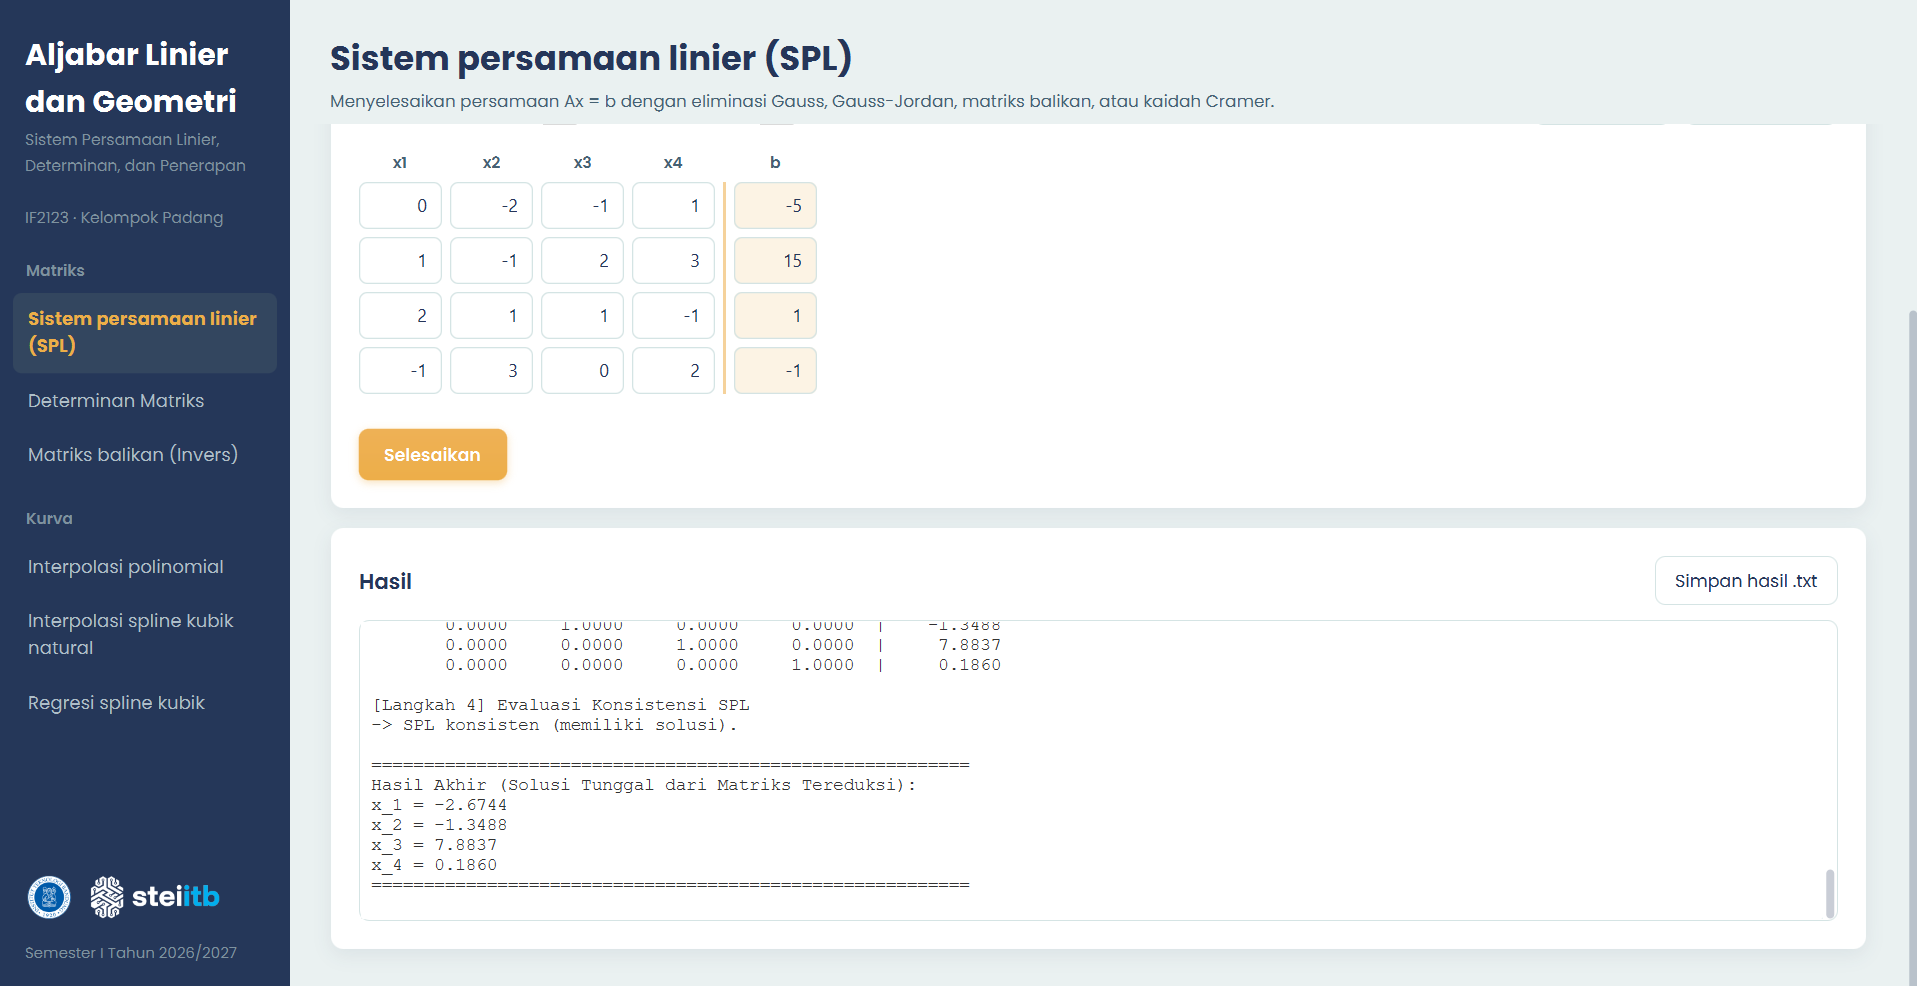
\includegraphics[width=0.8\textwidth]{5.3.1.gaussjordan.png}
    \caption{Penyelesaian SPL dengan Metode Gauss-Jordan}
\end{figure}
\begin{figure}[H]
    \centering
    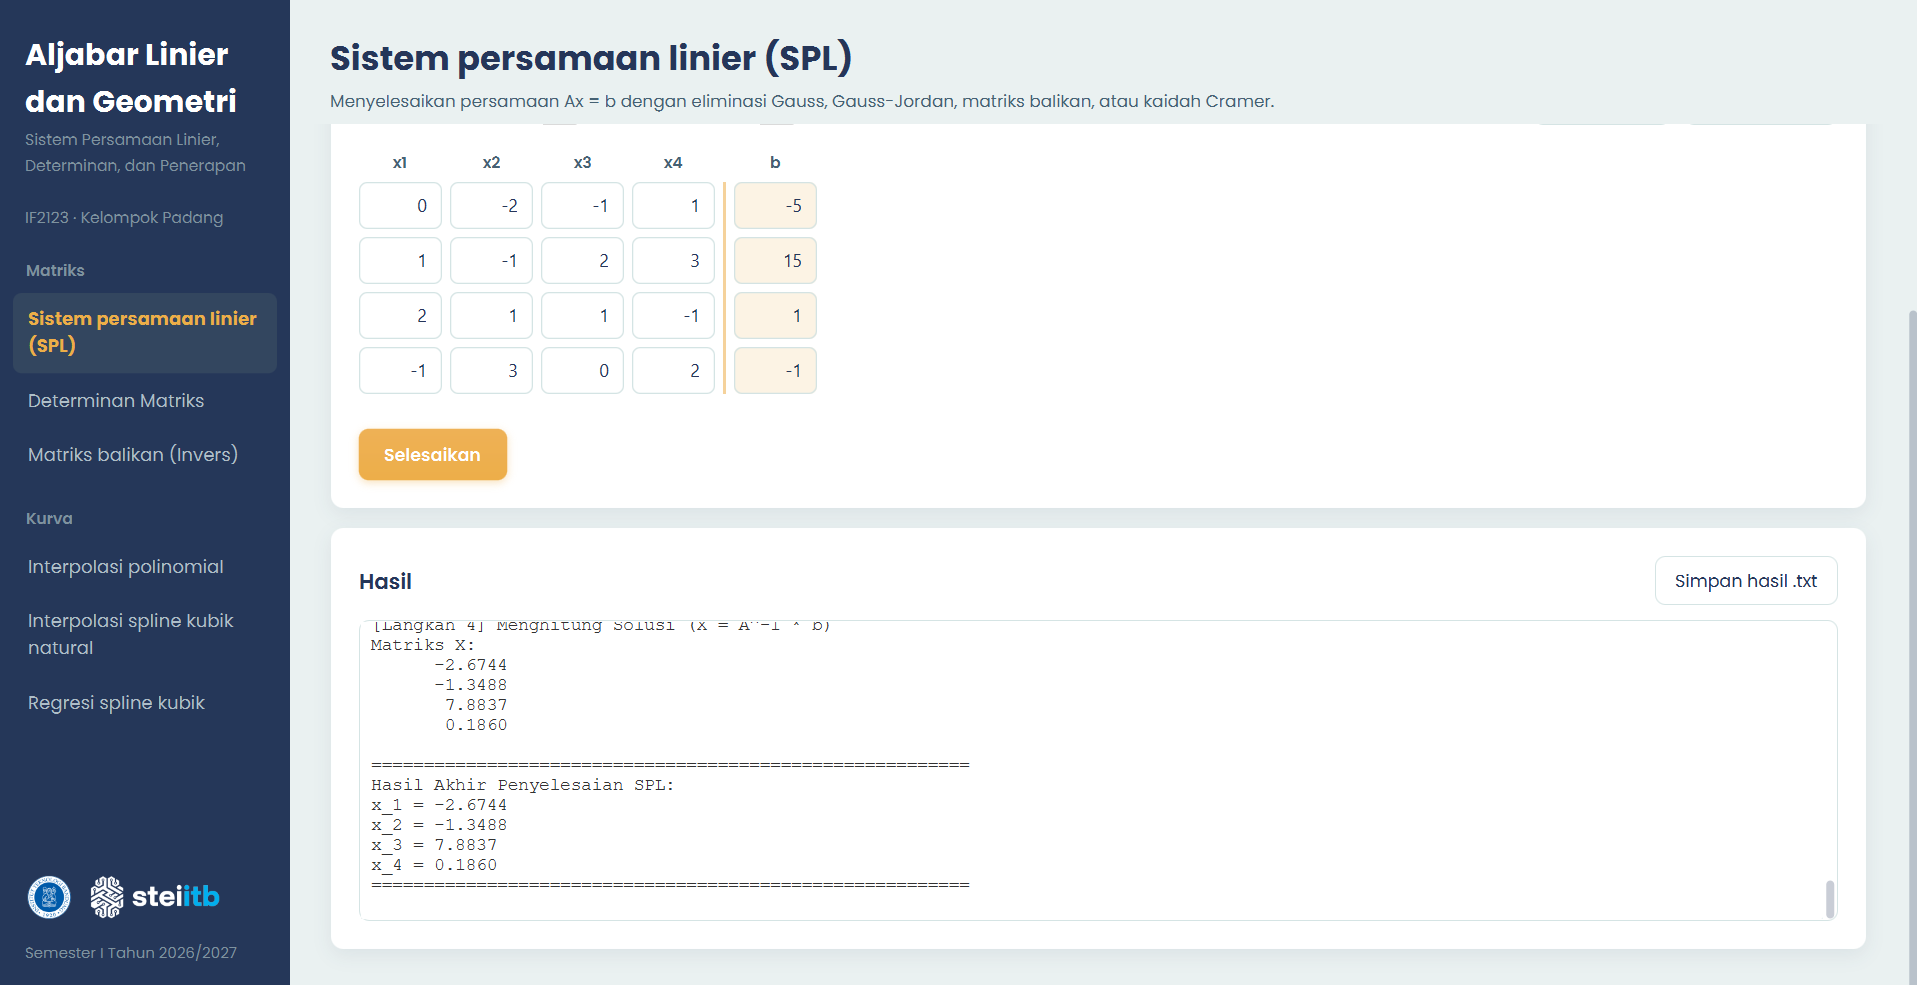
\includegraphics[width=0.8\textwidth]{5.3.1.invers.png}
    \caption{Penyelesaian SPL dengan Metode Invers}
\end{figure}
\begin{figure}[H]
    \centering
    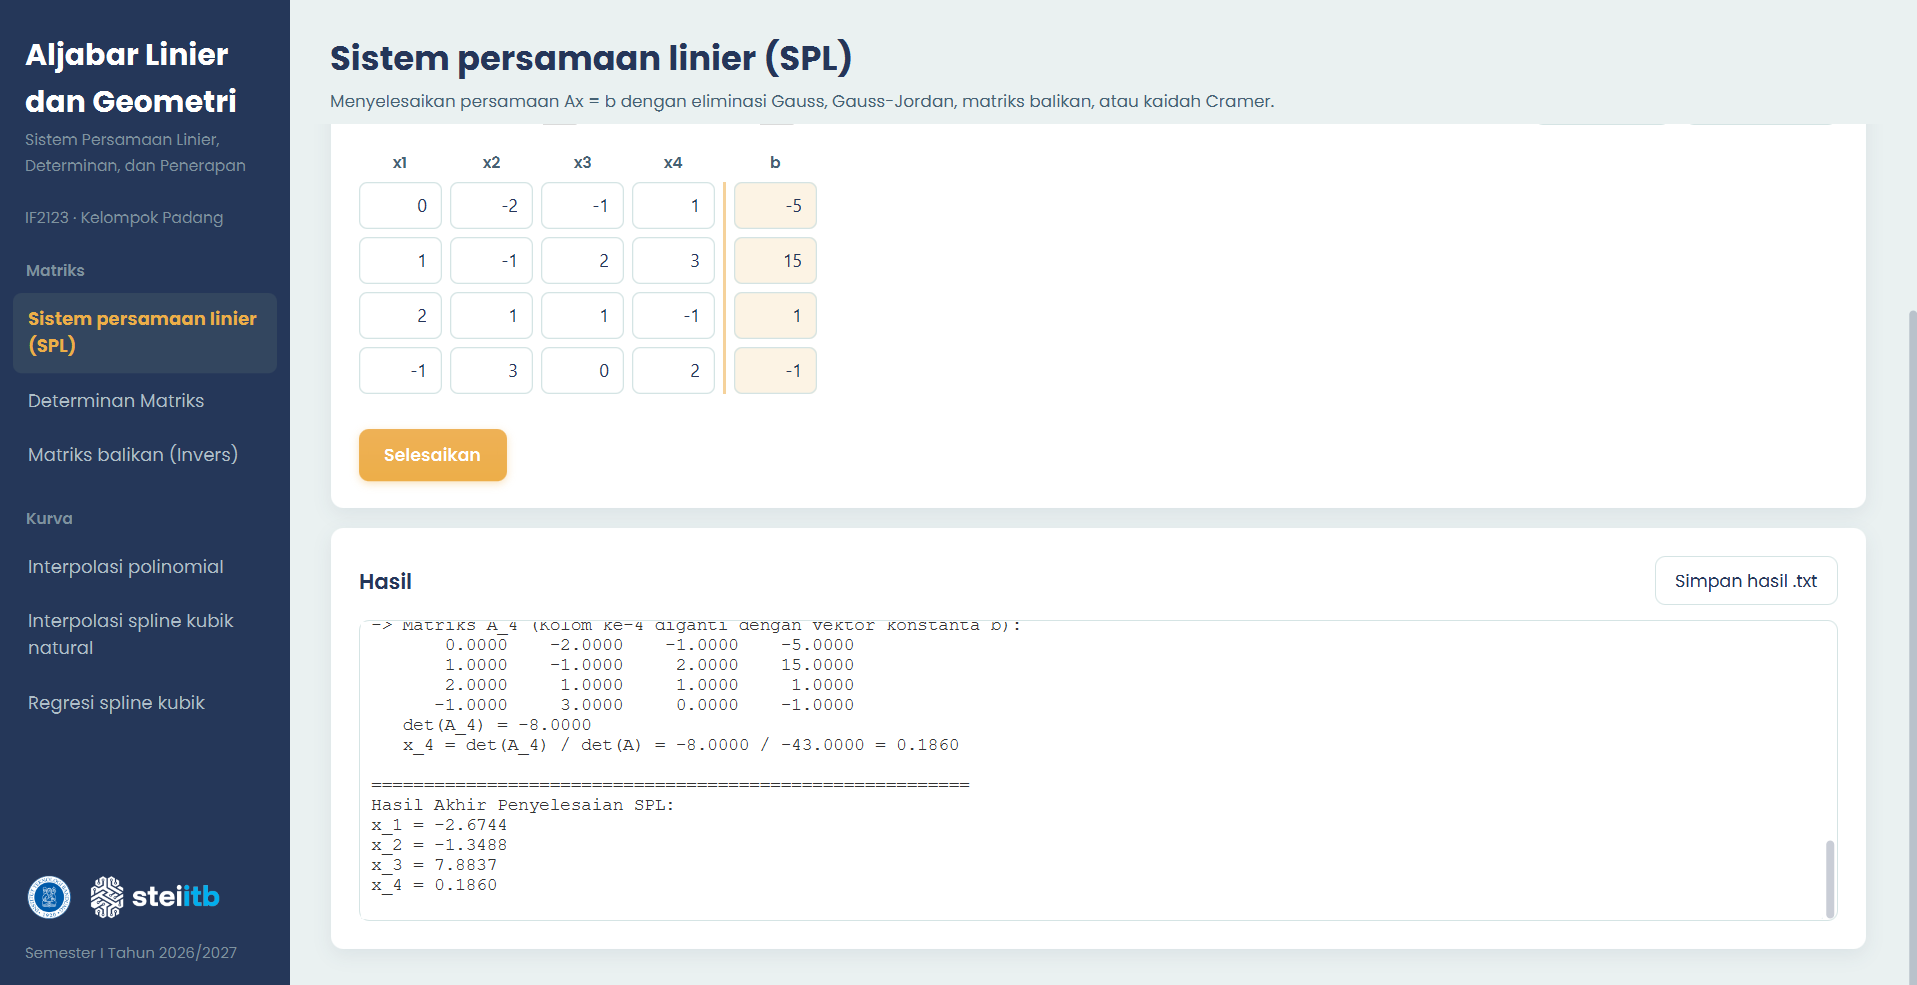
\includegraphics[width=0.8\textwidth]{5.3.1.cramer.png}
    \caption{Penyelesaian SPL dengan Kaidah Cramer}
\end{figure}

\textbf{Analisis:}
Seluruh metode, yaitu Eliminasi Gauss, Gauss-Jordan, Kaidah Cramer, dan Matriks Balikan, menghasilkan solusi tunggal yang konsisten. Karena determinan matriks koefisien tidak bernilai nol, matriks memiliki invers sehingga Kaidah Cramer dan Metode Matriks Balikan dapat diterapkan secara valid.

\subsection{Kasus Uji 4.3.2: Matriks $A$ Berukuran $3 \times 5$}
\textbf{Matriks Masukan:}
\[
A = \begin{bmatrix}
1 & 2 & -1 & 0 & 3 \\
2 & 4 & 1 & -1 & 5 \\
-1 & -2 & 2 & 3 & -1
\end{bmatrix}, \quad
b = \begin{bmatrix}
2 \\
10 \\
-1
\end{bmatrix}
\]

\textbf{Hasil Eksekusi Program:}
\begin{figure}[H]
    \centering
    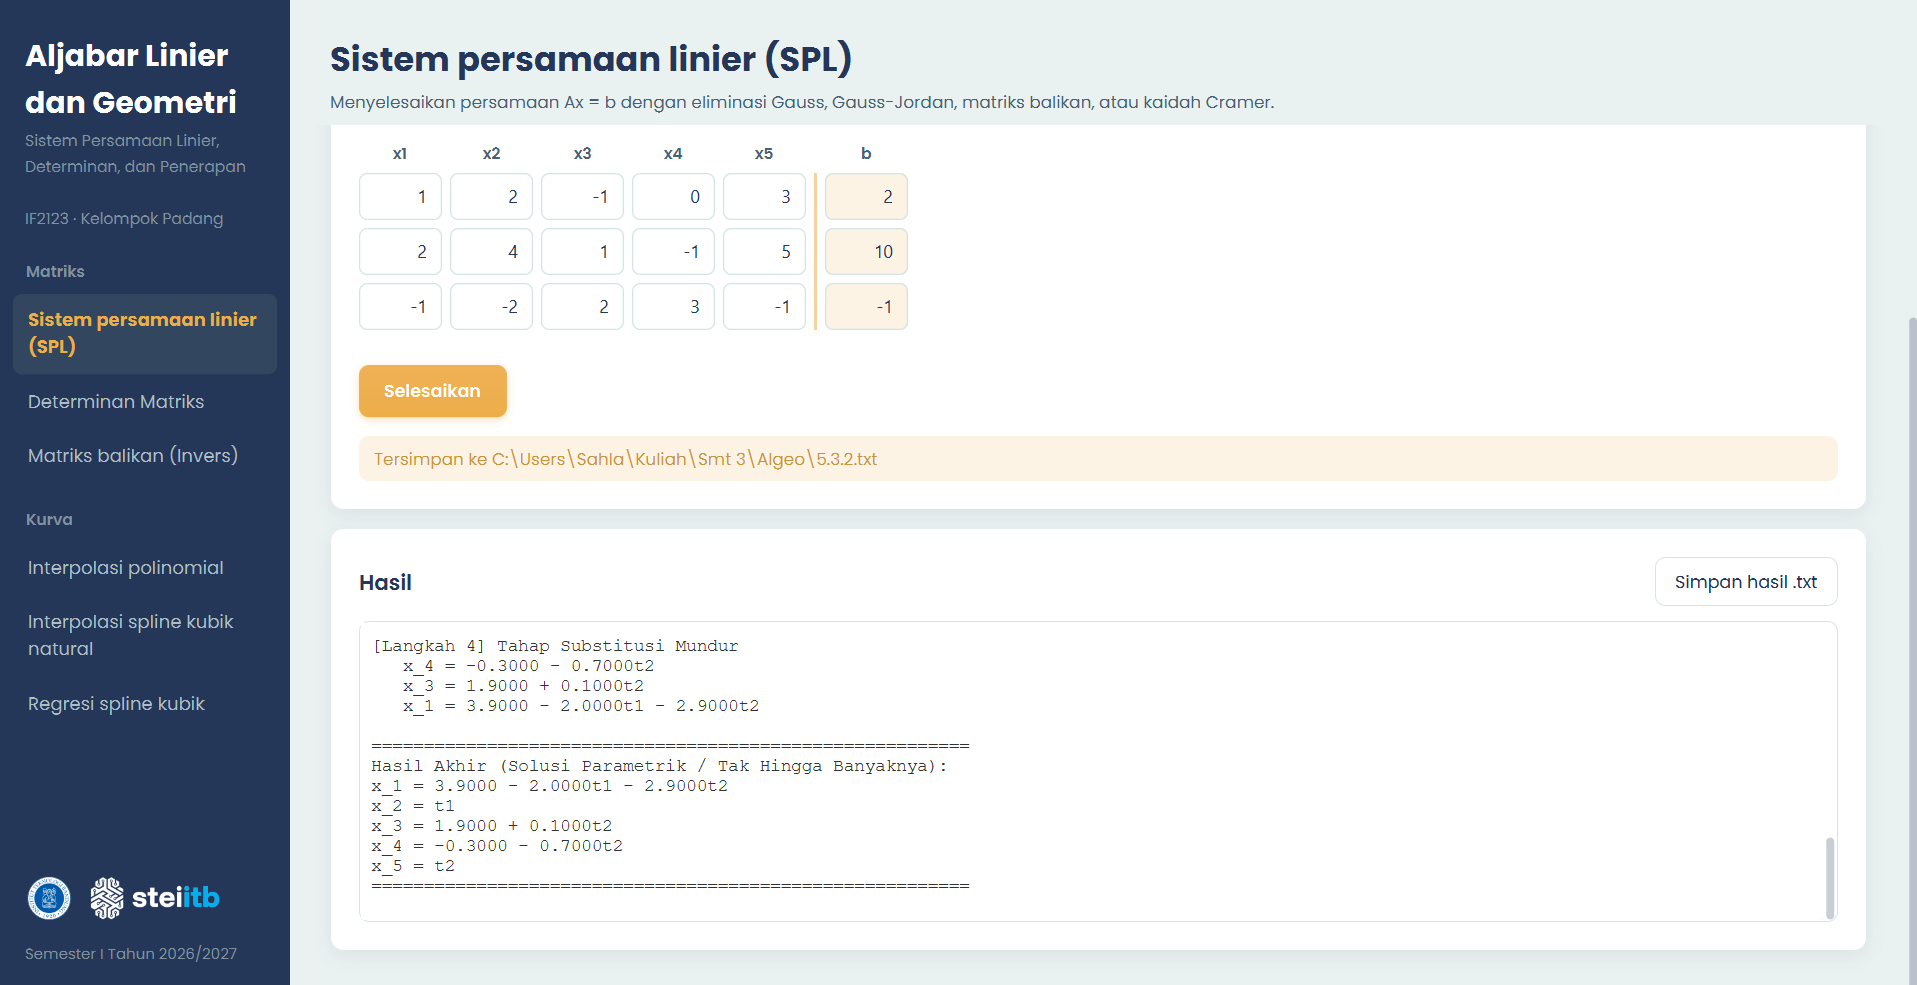
\includegraphics[width=0.8\textwidth]{5.3.2.gauss.png}
    \caption{Penyelesaian SPL dengan Metode Gauss}
\end{figure}
\begin{figure}[H]
    \centering
    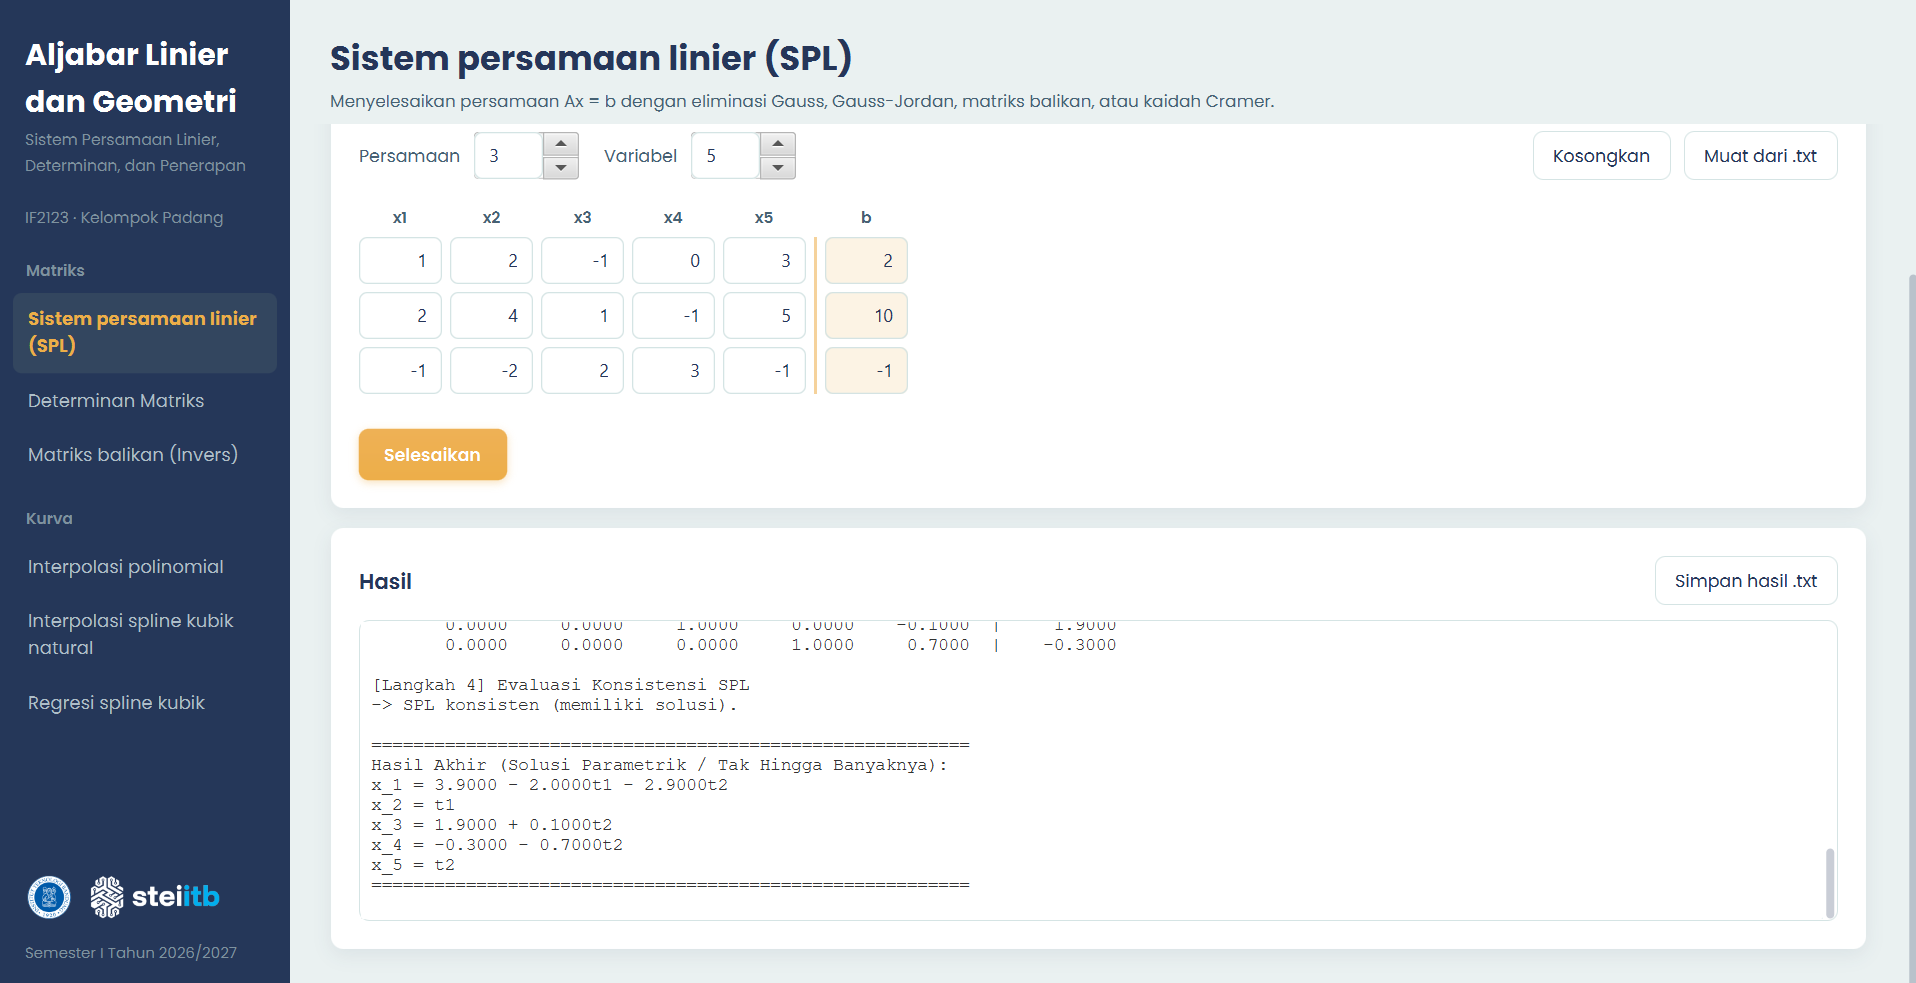
\includegraphics[width=0.8\textwidth]{5.3.2.gaussjordan.png}
    \caption{Penyelesaian SPL dengan Metode Gauss-Jordan}
\end{figure}
\begin{figure}[H]
    \centering
    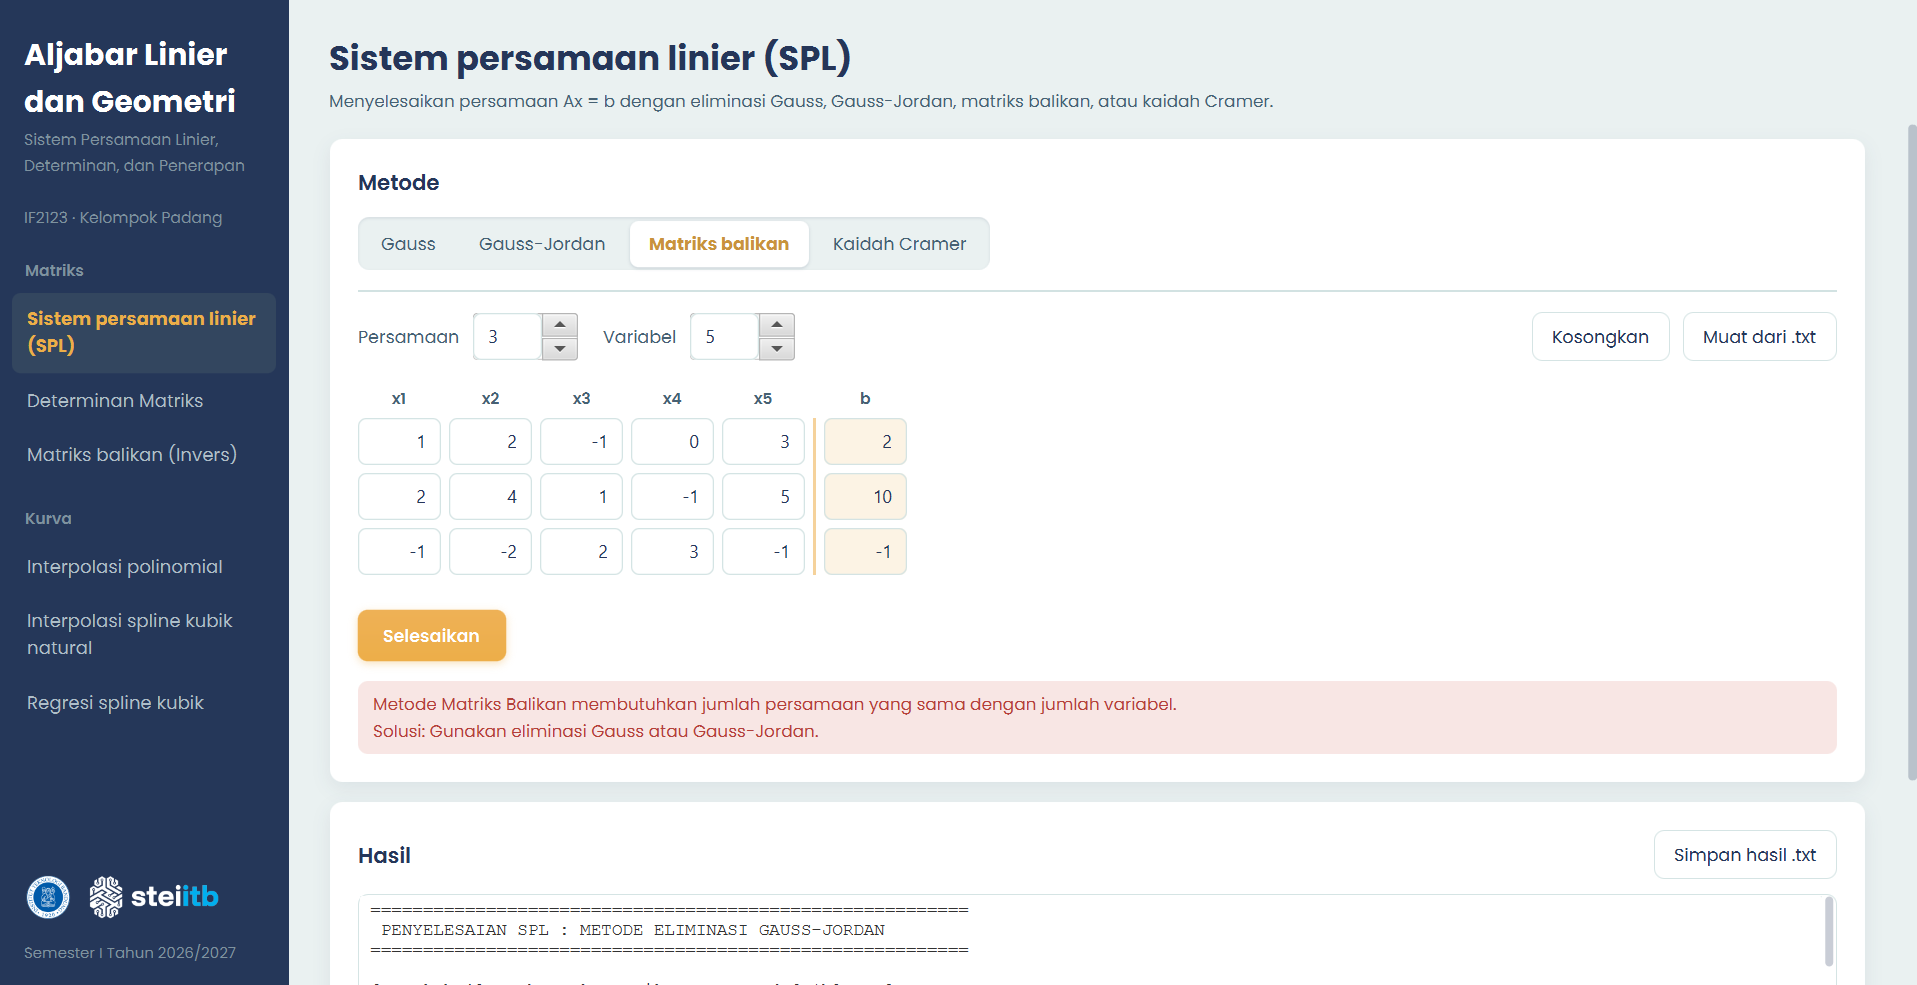
\includegraphics[width=0.8\textwidth]{5.3.2.invers.png}
    \caption{Penyelesaian SPL dengan Metode Invers}
\end{figure}
\begin{figure}[H]
    \centering
    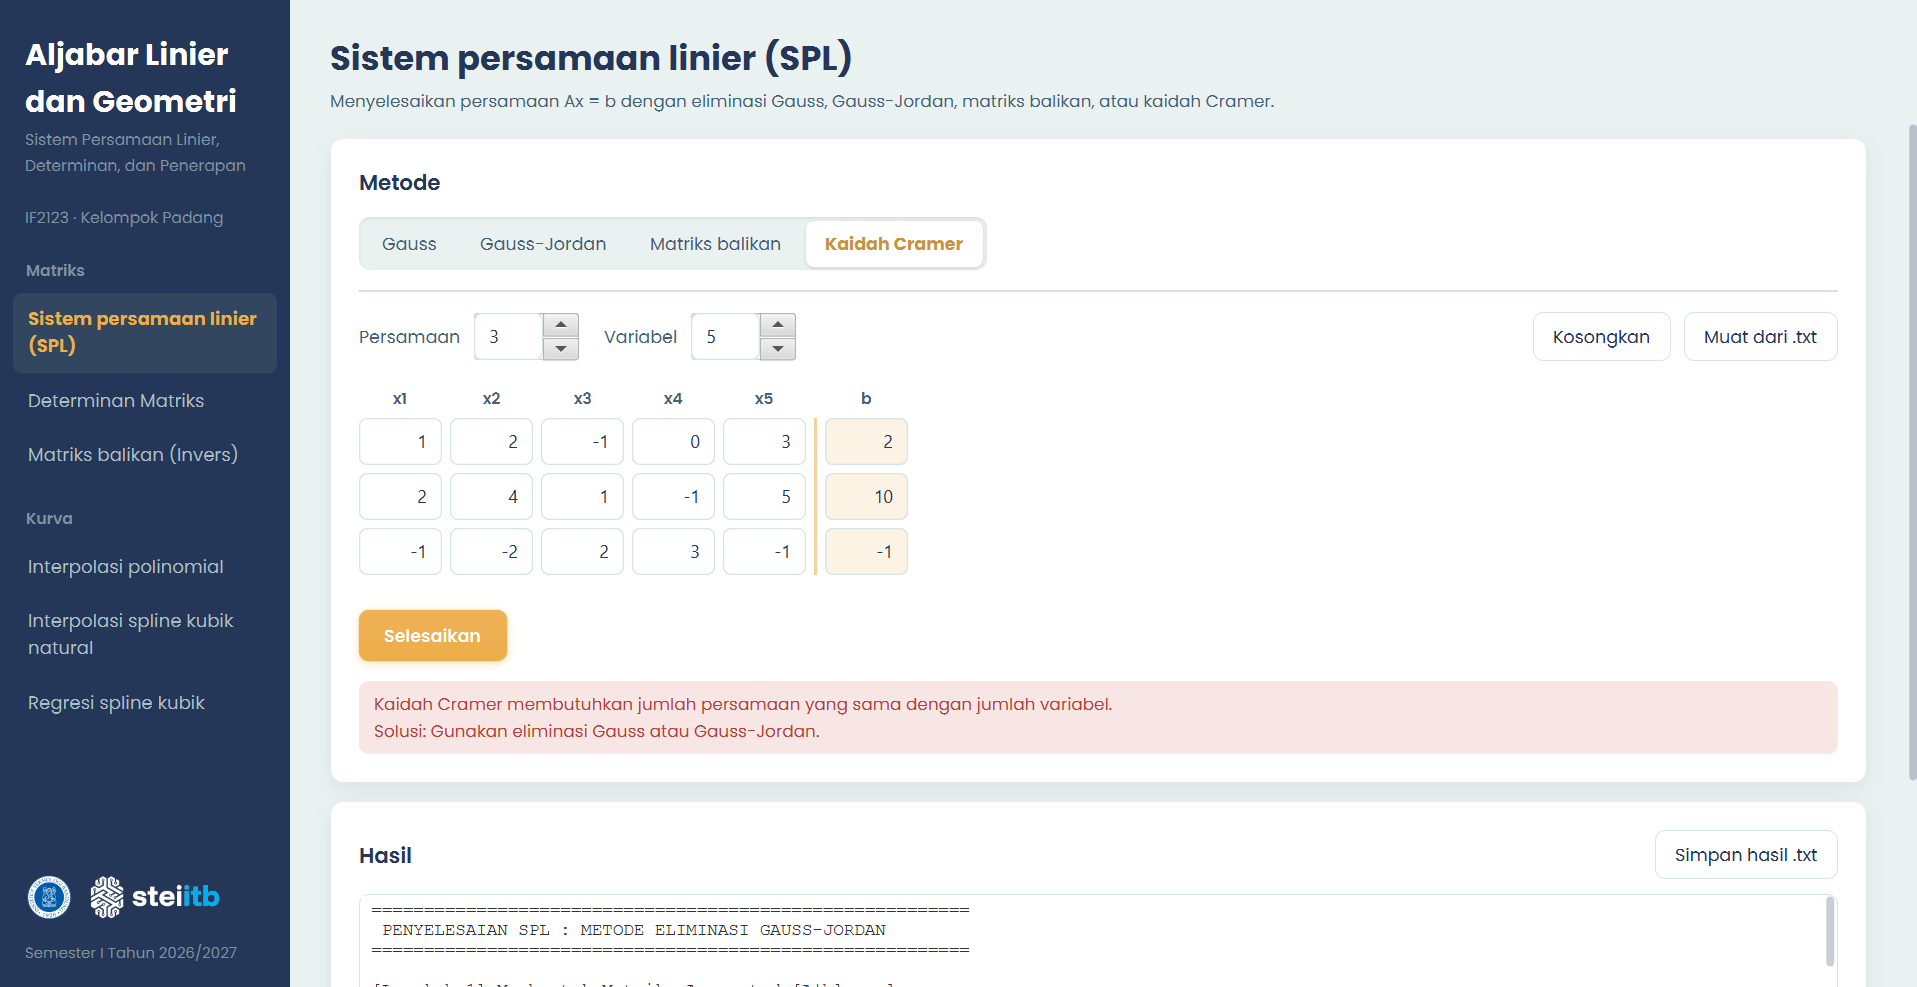
\includegraphics[width=0.8\textwidth]{5.3.2.cramer.png}
    \caption{Penyelesaian SPL dengan Kaidah Cramer}
\end{figure}

\textbf{Analisis:}
Matriks \(A\) berukuran \(3 \times 5\), jumlah variabel yang lebih banyak daripada persamaan tidak memenuhi syarat Kaidah Cramer dan Metode Matriks Balikan sehingga metode yang dapat digunakan hanya metode Eliminasi Gauss dan Gauss-Jordan.

\subsection{Kasus Uji 4.3.3: Matriks $A$ Berukuran $4 \times 4$}
\textbf{Matriks Masukan:}
\[
A = \begin{bmatrix}
1 & -2 & 3 & 1 \\
2 & 1 & -1 & 4 \\
0 & 3 & 2 & -2 \\
3 & -1 & 2 & 5
\end{bmatrix}, \quad
b = \begin{bmatrix}
4 \\
-1 \\
3 \\
4
\end{bmatrix}
\]

\textbf{Hasil Eksekusi Program:}
\begin{figure}[H]
    \centering
    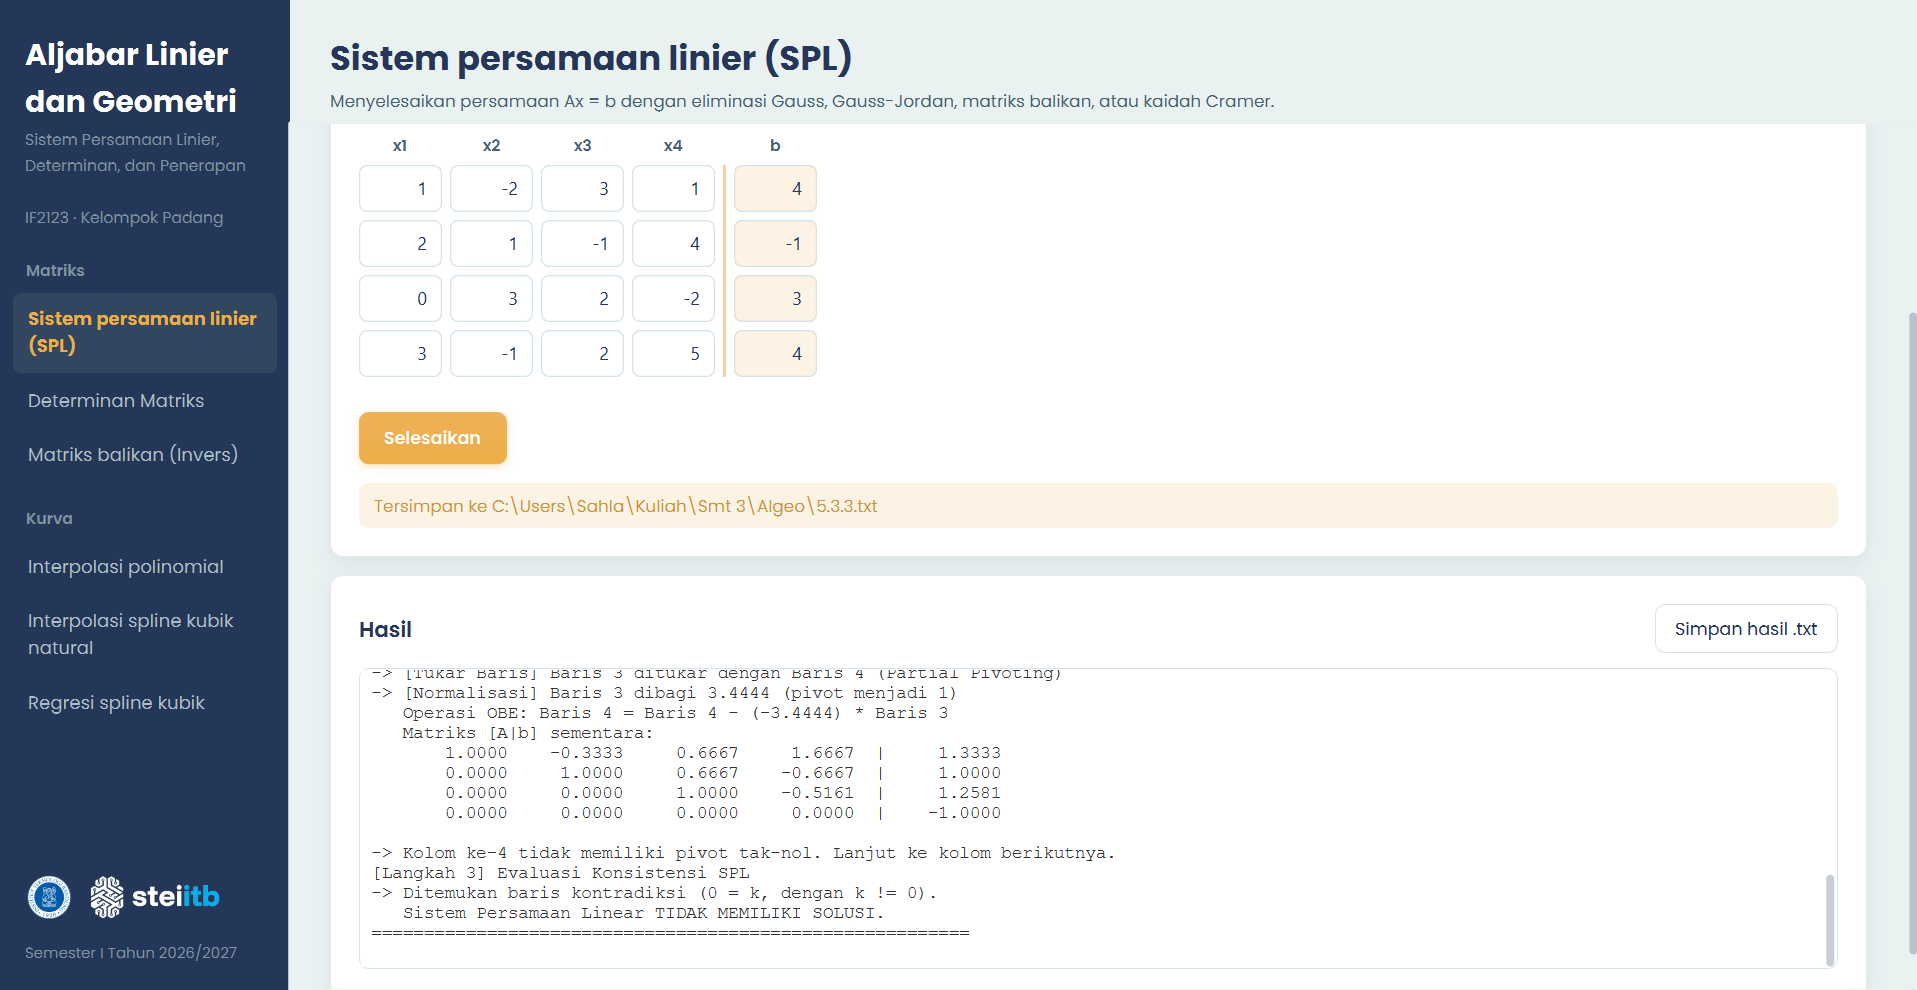
\includegraphics[width=0.8\textwidth]{5.3.3.gauss.png}
    \caption{Penyelesaian SPL dengan Metode Gauss}
\end{figure}
\begin{figure}[H]
    \centering
    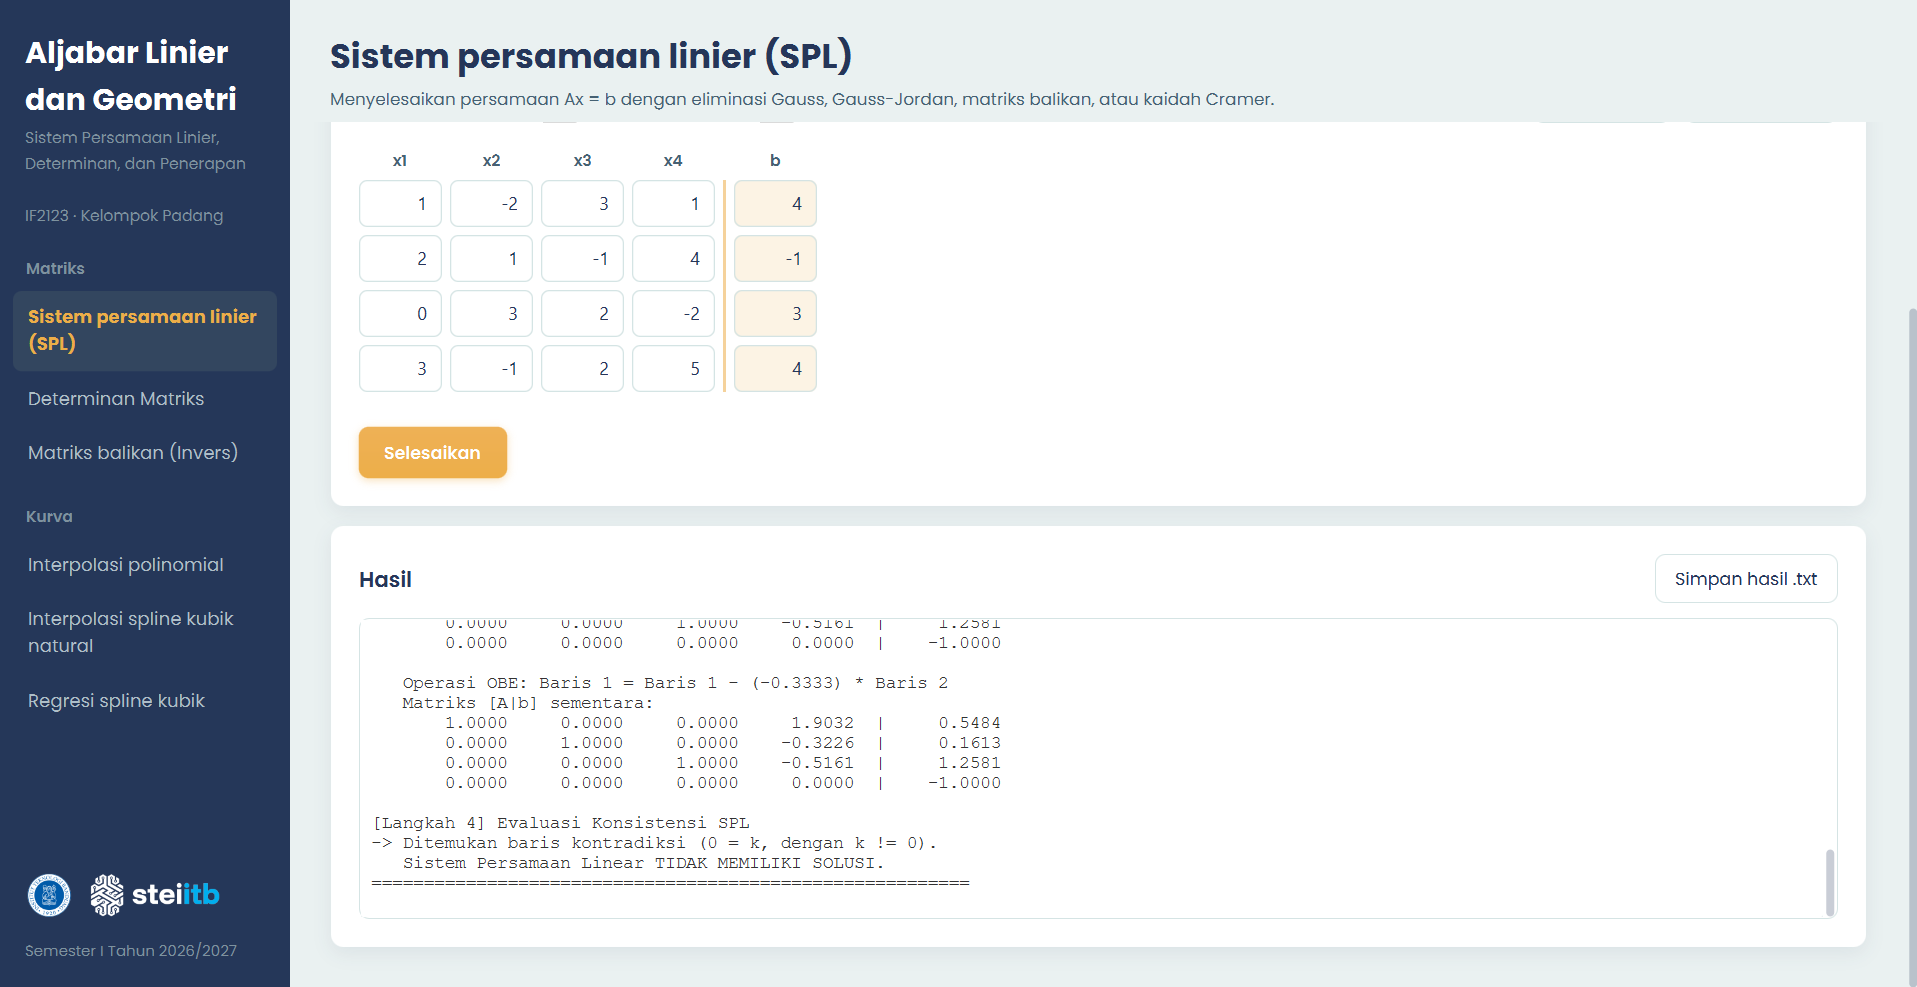
\includegraphics[width=0.8\textwidth]{5.3.3.gaussjordan.png}
    \caption{Penyelesaian SPL dengan Metode Gauss-Jordan}
\end{figure}
\begin{figure}[H]
    \centering
    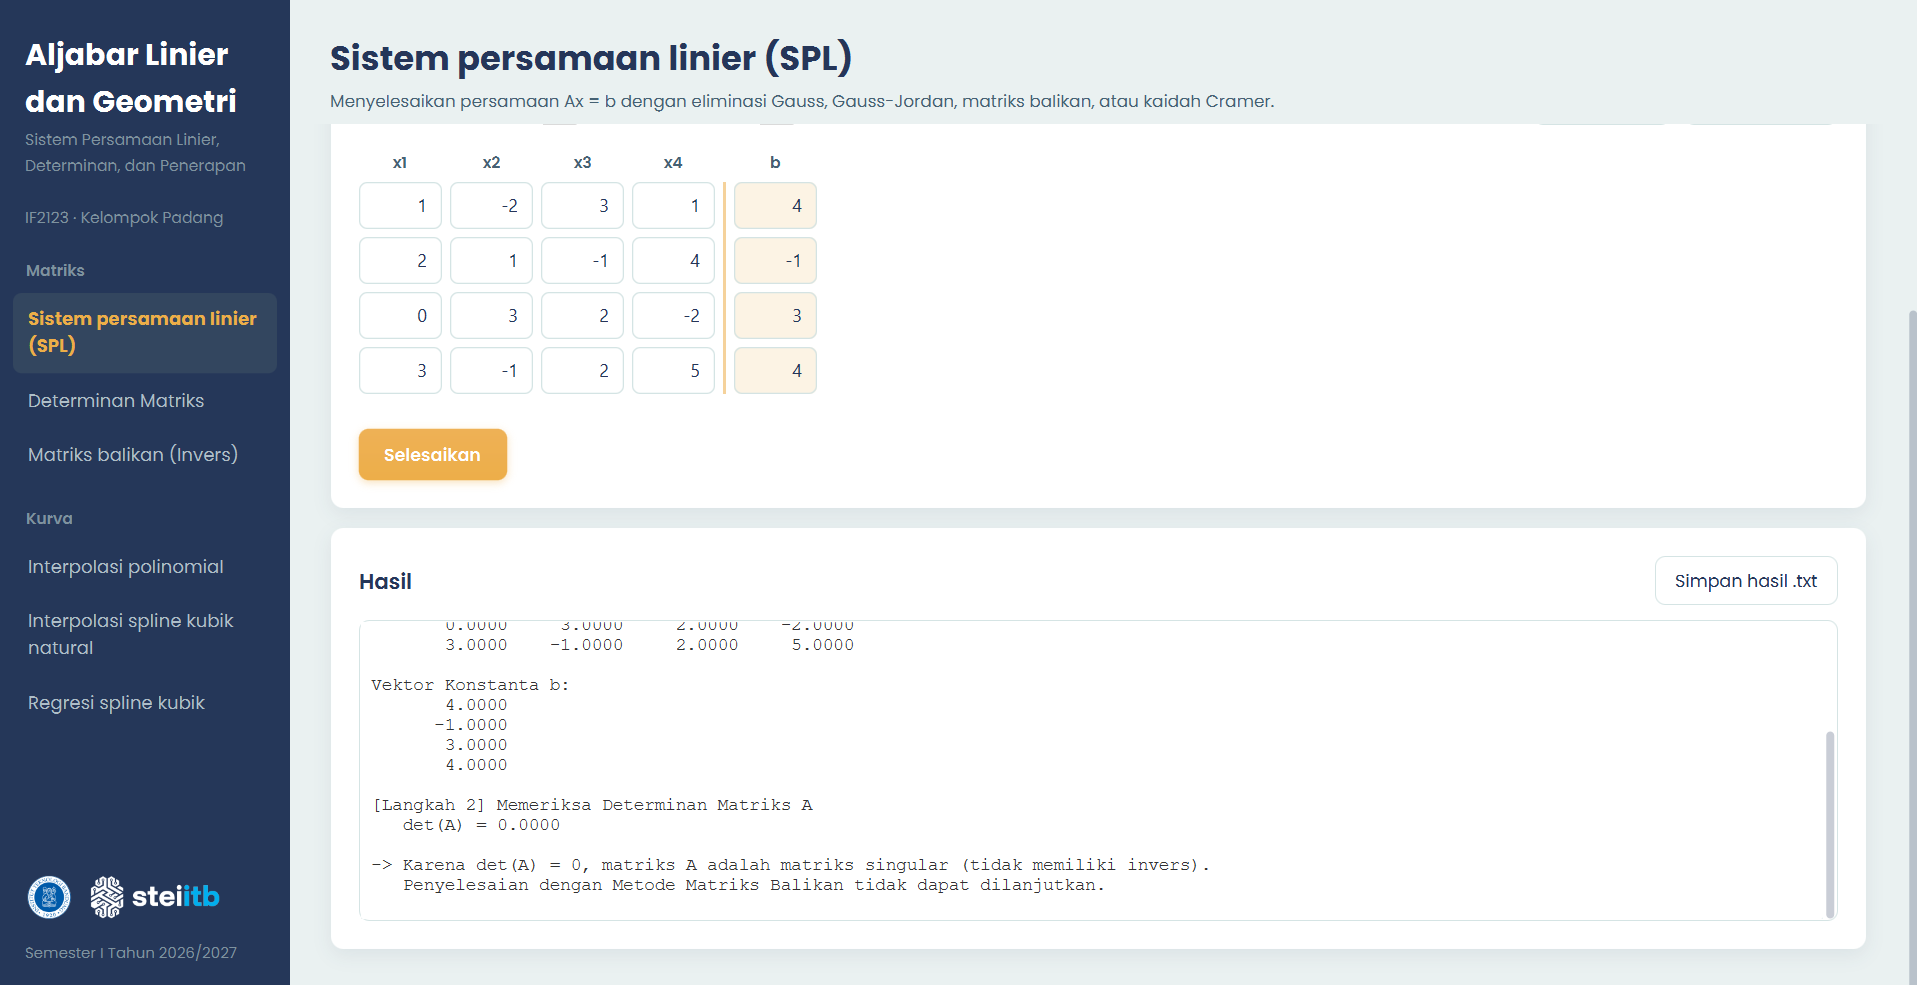
\includegraphics[width=0.8\textwidth]{5.3.3.invers.png}
    \caption{Penyelesaian SPL dengan Metode Invers}
\end{figure}
\begin{figure}[H]
    \centering
    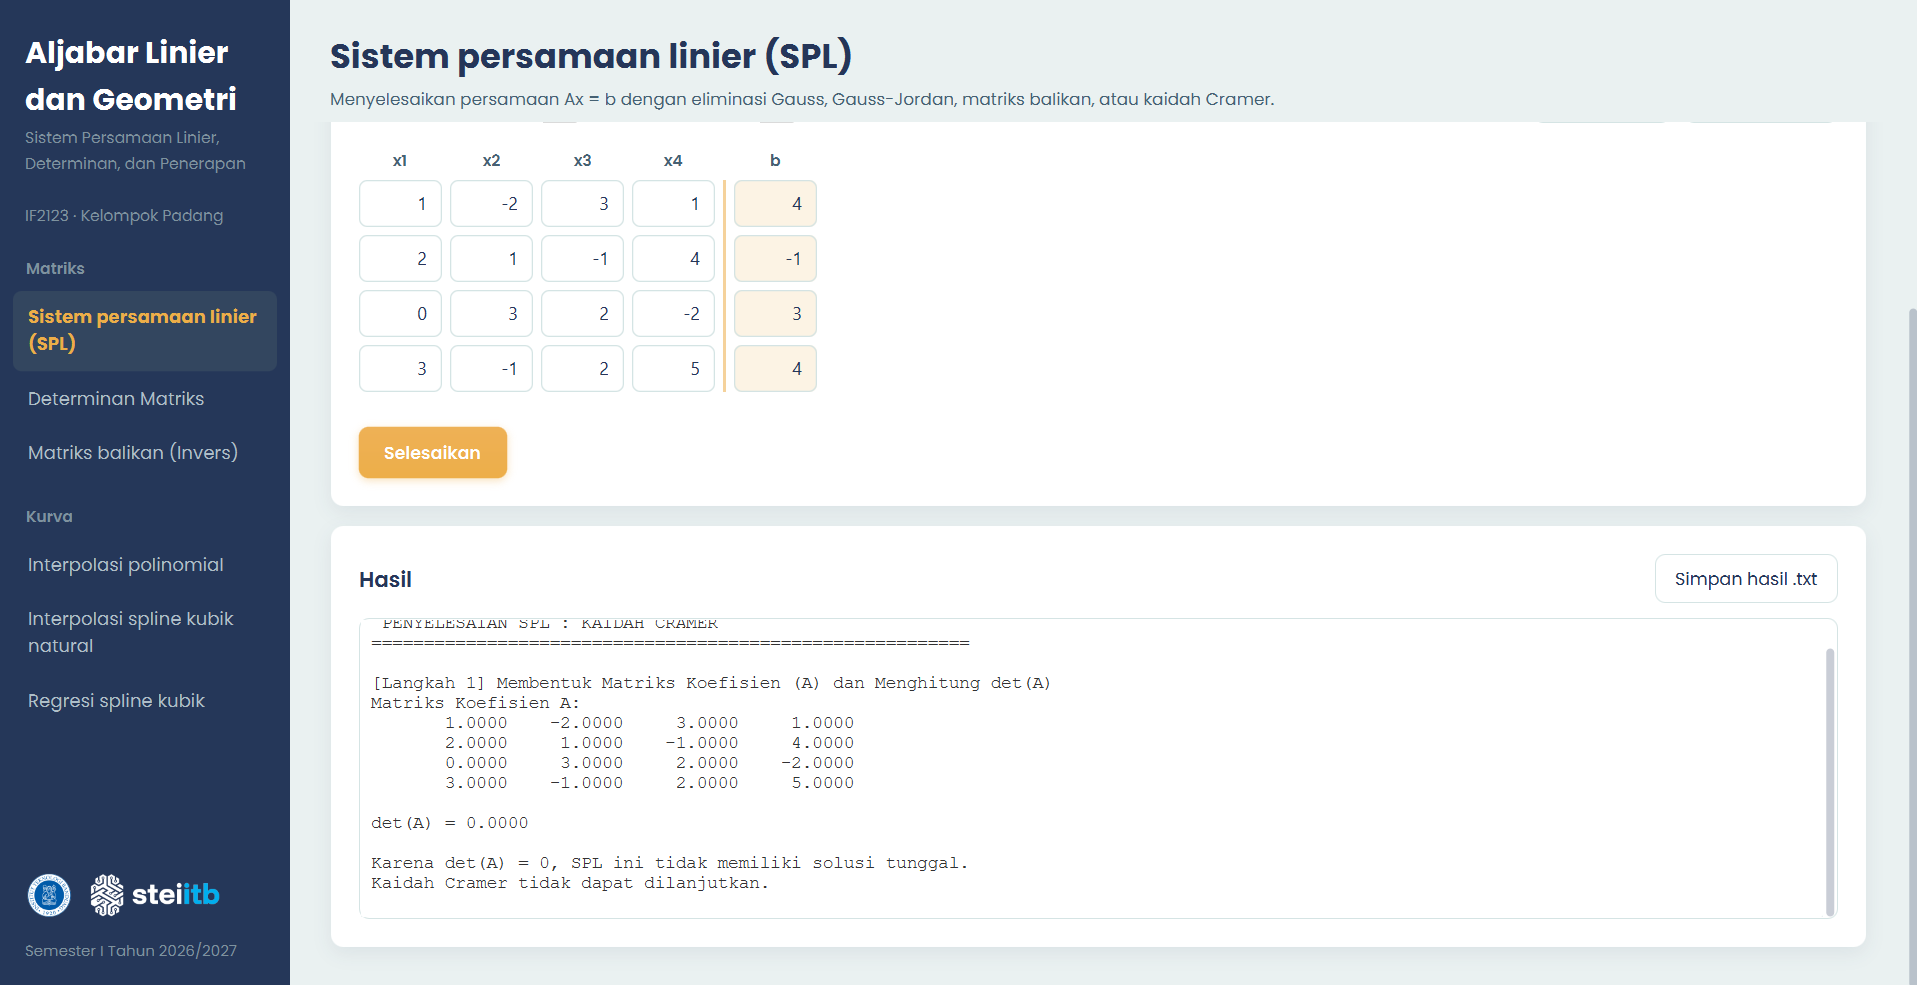
\includegraphics[width=0.8\textwidth]{5.3.3.cramer.png}
    \caption{Penyelesaian SPL dengan Kaidah Cramer}
\end{figure}

\textbf{Analisis:}
Berdasarkan hasil perhitungan dari metode Eliminasi Gauss dan Gauss-Jordan, matriks \(A\) tidak memiliki solusi dan memiliki \(determinan = 0\) sehingga metode Kaidah Cramer dan Metode Matriks Balikan tidak dapat digunakan.

\subsection{Kasus Uji 4.3.4: Matriks \textit{discrete Laplacian} satu dimensi}

\subsubsection{Kasus Uji 4.3.4.1: Matriks \(n = 6\)}
\textbf{Matriks Masukan:}
\[
A_6 = \begin{bmatrix}
2 & -1 & 0 & 0 & 0 & 0 \\
-1 & 2 & -1 & 0 & 0 & 0 \\
0 & -1 & 2 & -1 & 0 & 0 \\
0 & 0 & -1 & 2 & -1 & 0 \\
0 & 0 & 0 & -1 & 2 & -1 \\
0 & 0 & 0 & 0 & -1 & 2
\end{bmatrix}, \quad
b_6 = \begin{bmatrix}
1 \\
1 \\
1 \\
1 \\
1 \\
1
\end{bmatrix}
\]

\textbf{Hasil Eksekusi Program:}
\begin{figure}[H]
    \centering
    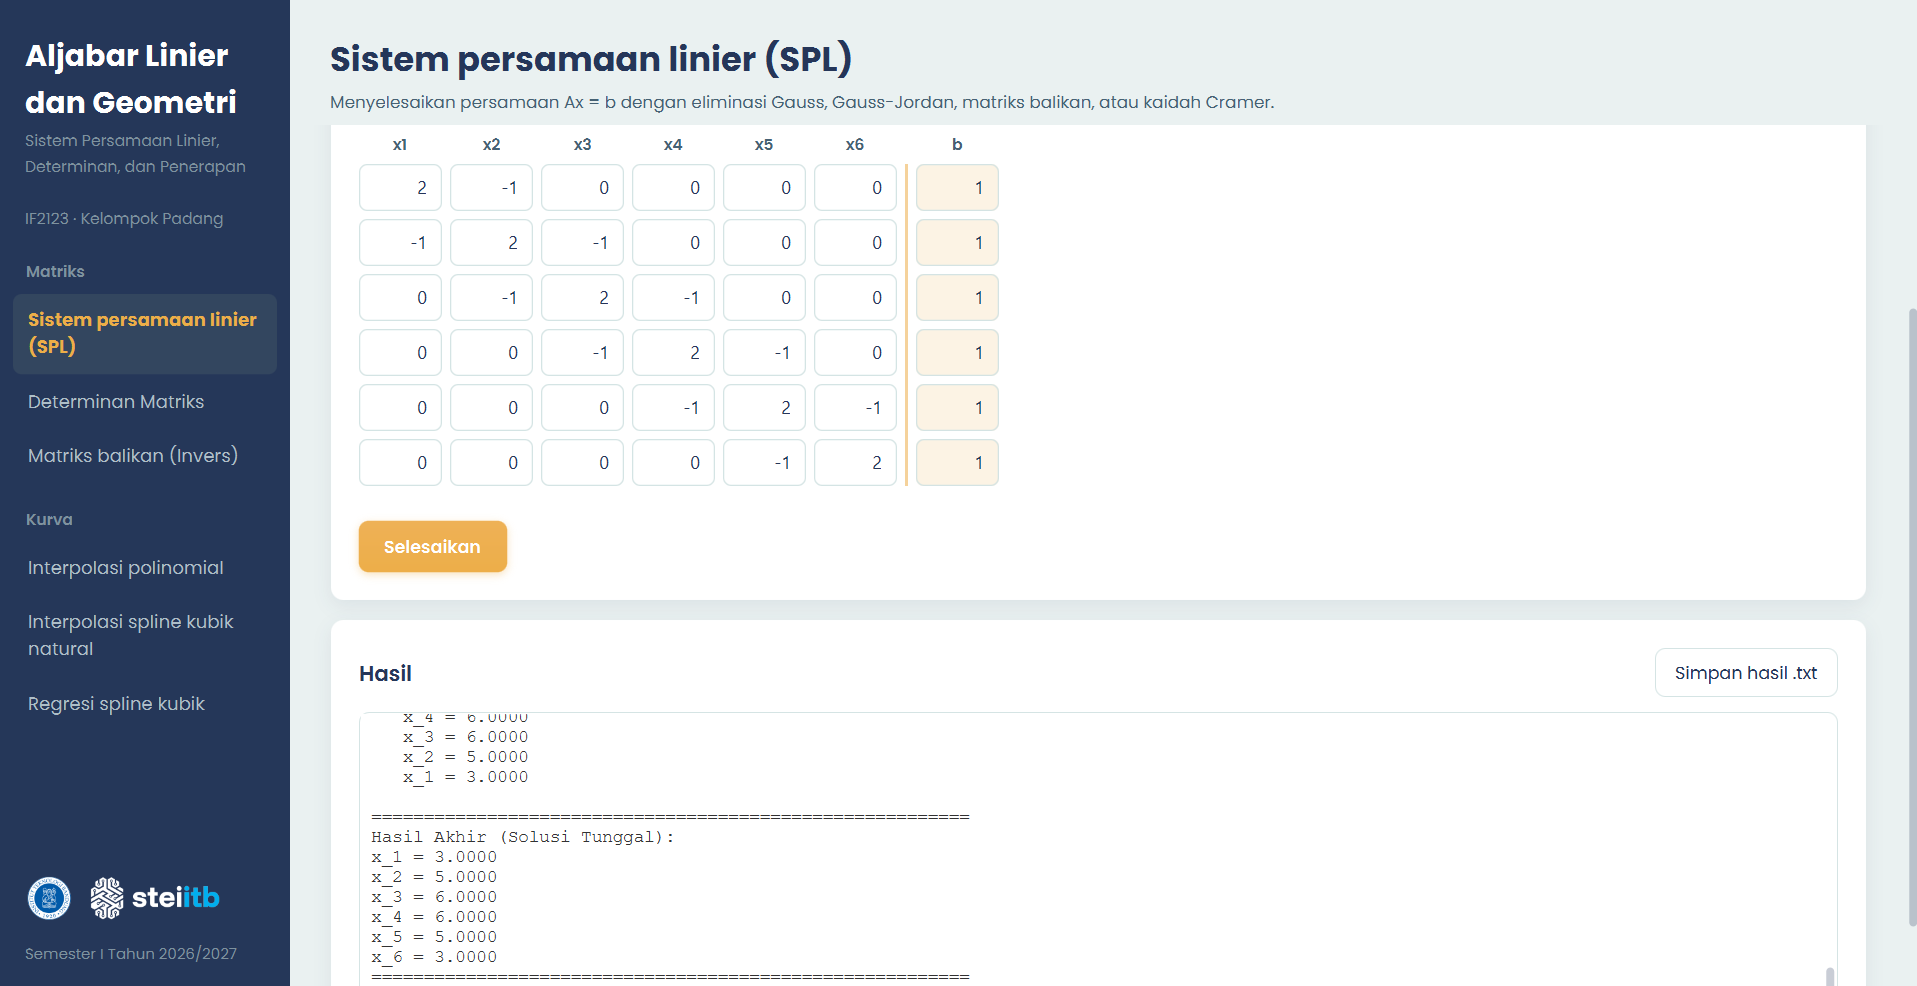
\includegraphics[width=0.8\textwidth]{5.3.4.1.gauss.png}
    \caption{Penyelesaian SPL dengan Metode Gauss}
\end{figure}
\begin{figure}[H]
    \centering
    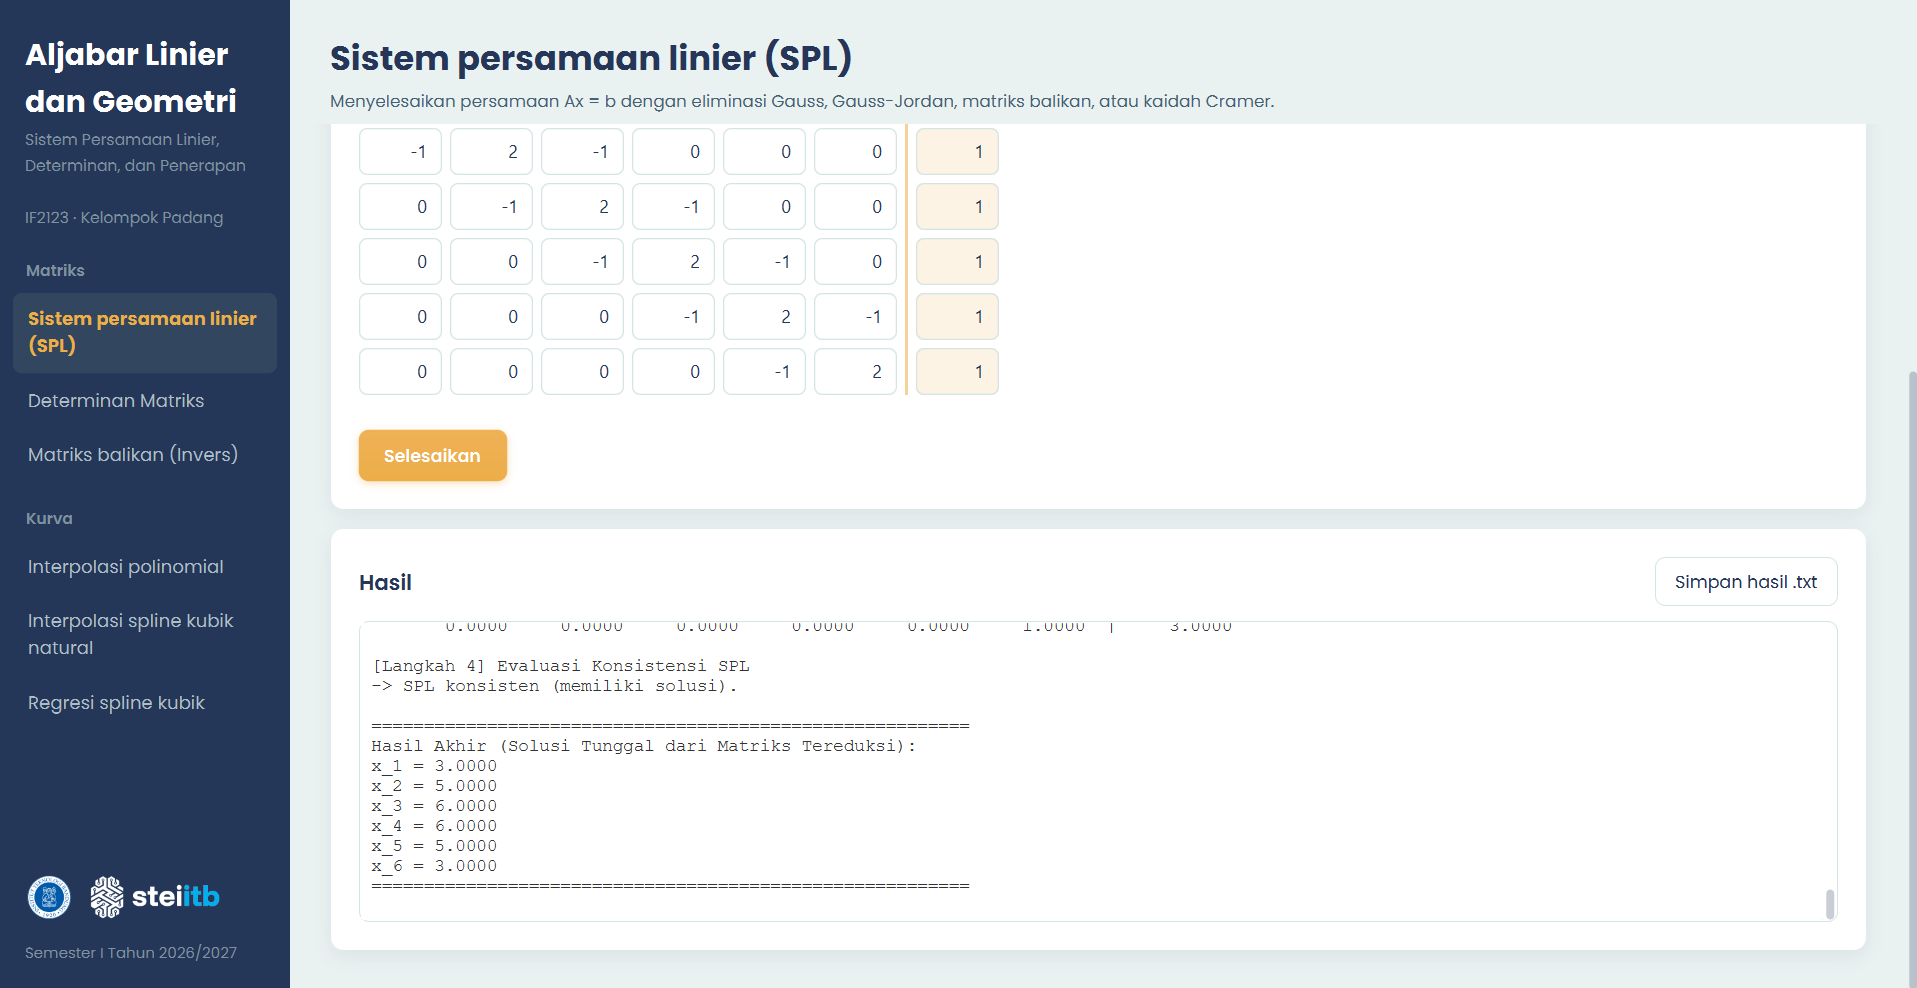
\includegraphics[width=0.8\textwidth]{5.3.4.1.gaussjordan.png}
    \caption{Penyelesaian SPL dengan Metode Gauss-Jordan}
\end{figure}
\begin{figure}[H]
    \centering
    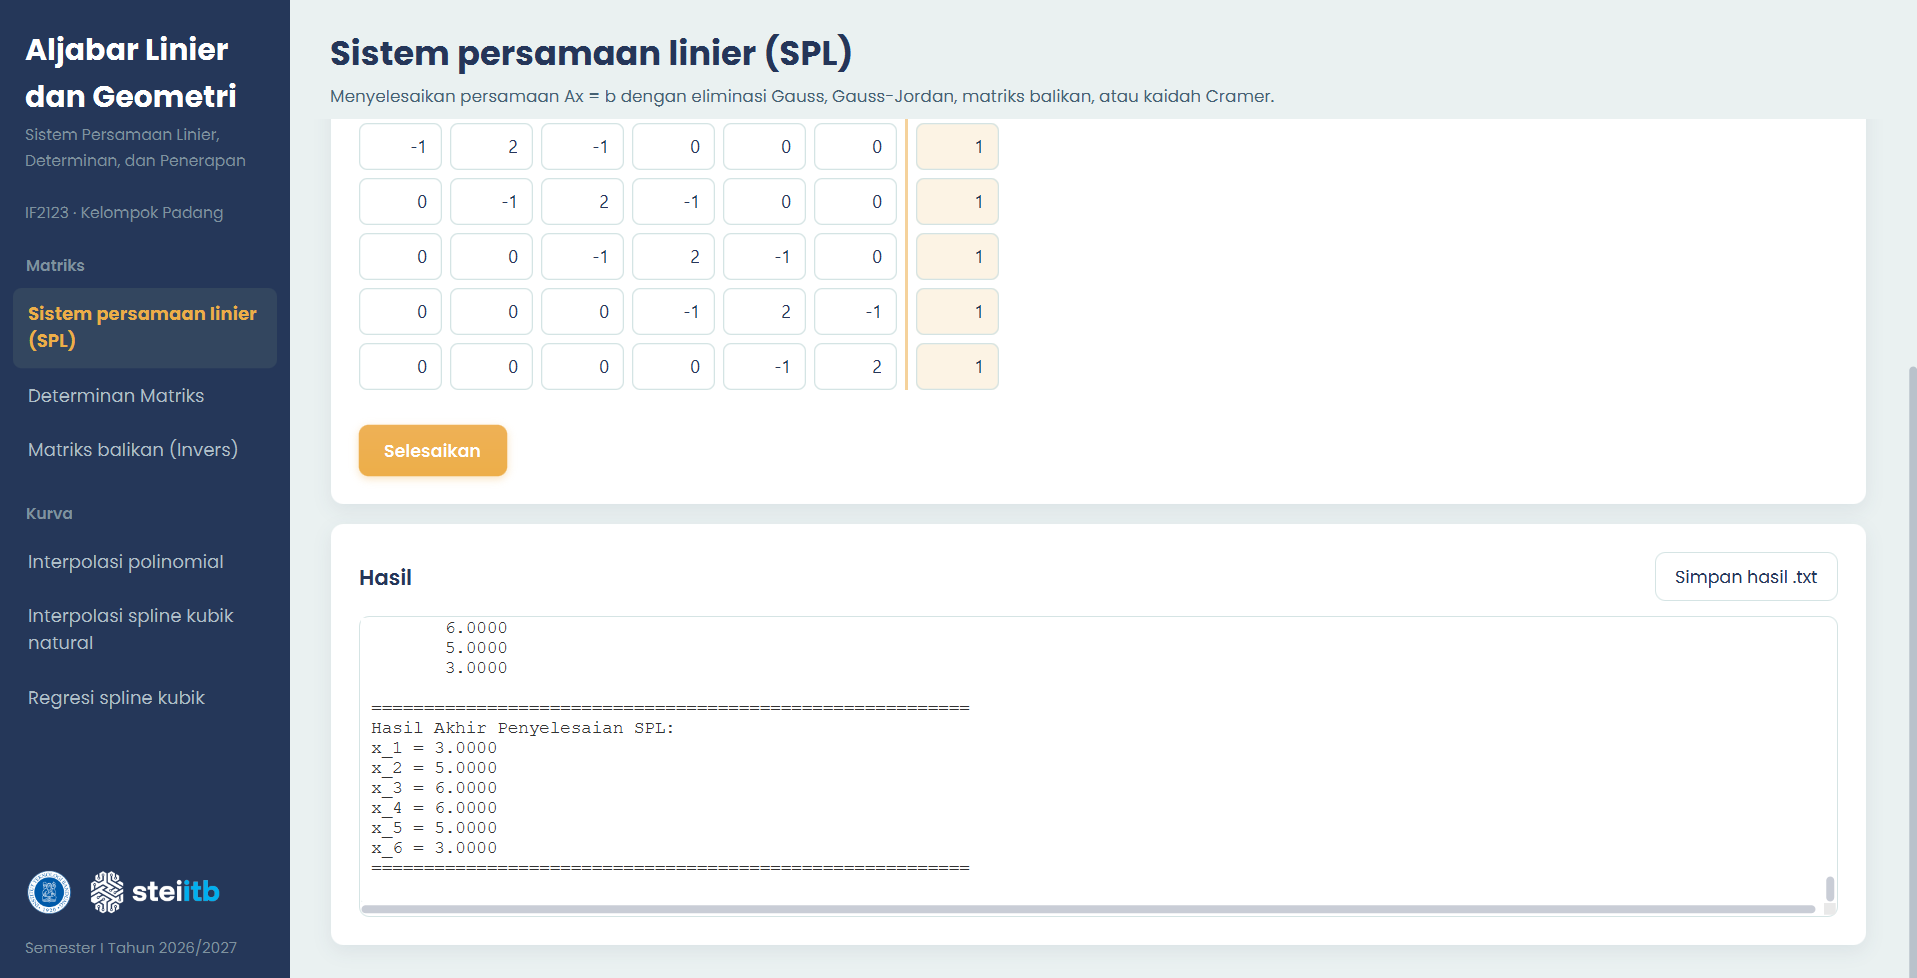
\includegraphics[width=0.8\textwidth]{5.3.4.1.invers.png}
    \caption{Penyelesaian SPL dengan Metode Invers}
\end{figure}
\begin{figure}[H]
    \centering
    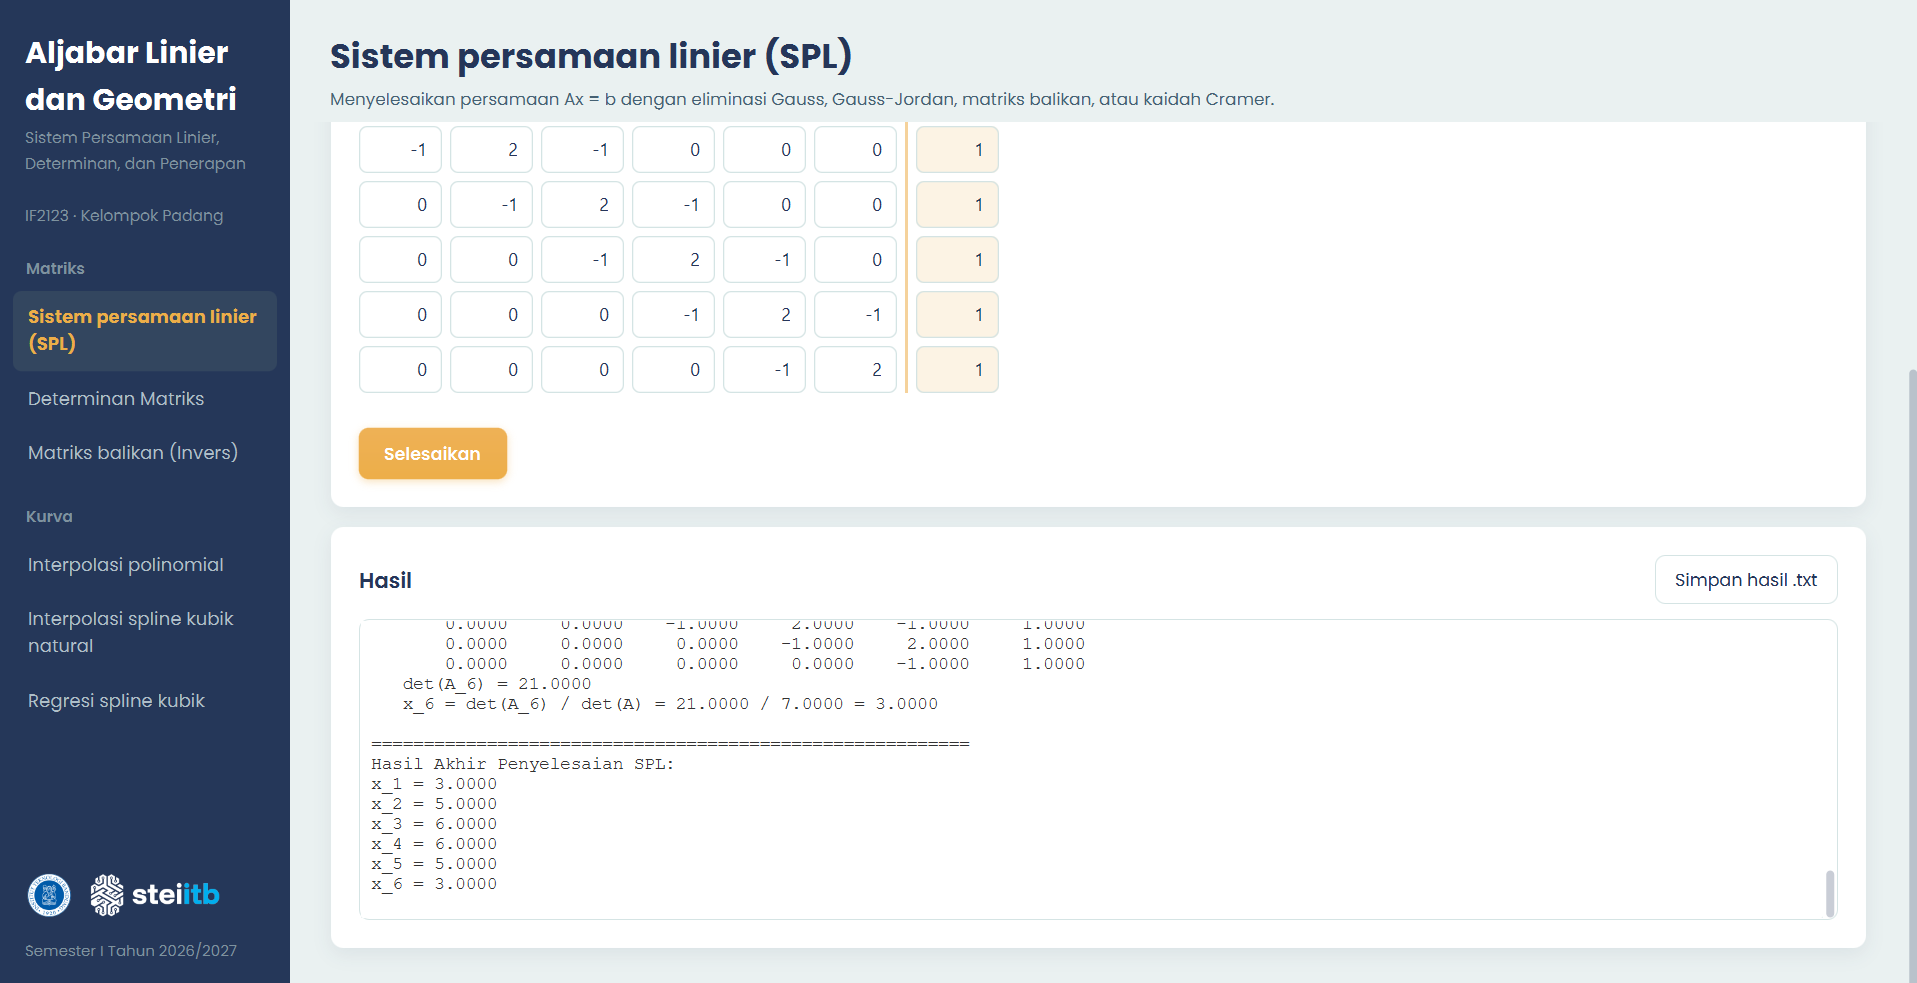
\includegraphics[width=0.8\textwidth]{5.3.4.1.cramer.png}
    \caption{Penyelesaian SPL dengan Kaidah Cramer}
\end{figure}

\textbf{Analisis:}
Seluruh metode, yaitu Eliminasi Gauss, Gauss-Jordan, Kaidah Cramer, dan Matriks Balikan, menghasilkan solusi tunggal yang konsisten. Karena determinan matriks koefisien tidak bernilai nol, matriks memiliki invers sehingga Kaidah Cramer dan Metode Matriks Balikan dapat diterapkan secara valid.

\subsubsection{Kasus Uji 4.3.4.2: Matriks \(n = 10\)}
\textbf{Matriks Masukan:}
\[
A_{10} = \begin{bmatrix}
2 & -1 & 0 & 0 & 0 & 0 & 0 & 0 & 0 & 0 \\
-1 & 2 & -1 & 0 & 0 & 0 & 0 & 0 & 0 & 0 \\
0 & -1 & 2 & -1 & 0 & 0 & 0 & 0 & 0 & 0 \\
0 & 0 & -1 & 2 & -1 & 0 & 0 & 0 & 0 & 0 \\
0 & 0 & 0 & -1 & 2 & -1 & 0 & 0 & 0 & 0 \\
0 & 0 & 0 & 0 & -1 & 2 & -1 & 0 & 0 & 0 \\
0 & 0 & 0 & 0 & 0 & -1 & 2 & -1 & 0 & 0 \\
0 & 0 & 0 & 0 & 0 & 0 & -1 & 2 & -1 & 0 \\
0 & 0 & 0 & 0 & 0 & 0 & 0 & -1 & 2 & -1 \\
0 & 0 & 0 & 0 & 0 & 0 & 0 & 0 & -1 & 2
\end{bmatrix}, \quad
b_{10} = \begin{bmatrix}
1 \\
1 \\
1 \\
1 \\
1 \\
1 \\
1 \\
1 \\
1 \\
1
\end{bmatrix}
\]

\textbf{Hasil Eksekusi Program:}
\begin{figure}[H]
    \centering
    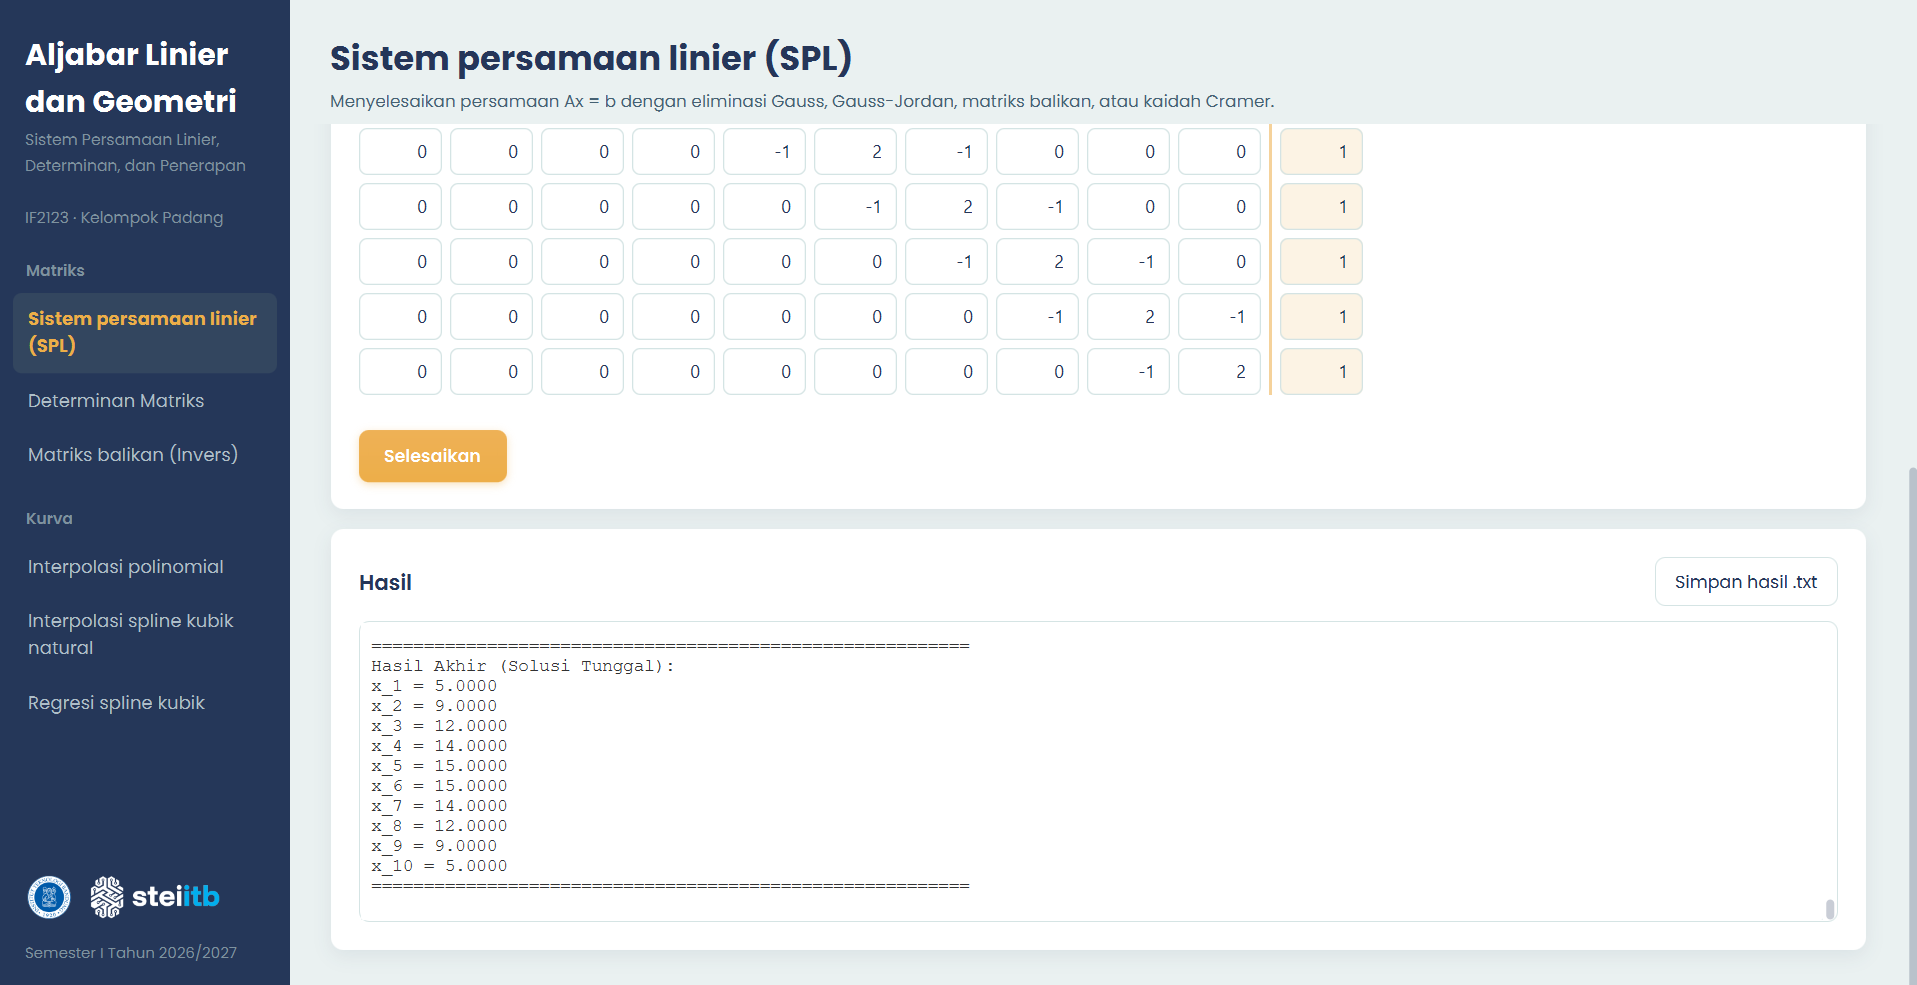
\includegraphics[width=0.8\textwidth]{5.3.4.2.gauss.png}
    \caption{Penyelesaian SPL dengan Metode Gauss}
\end{figure}
\begin{figure}[H]
    \centering
    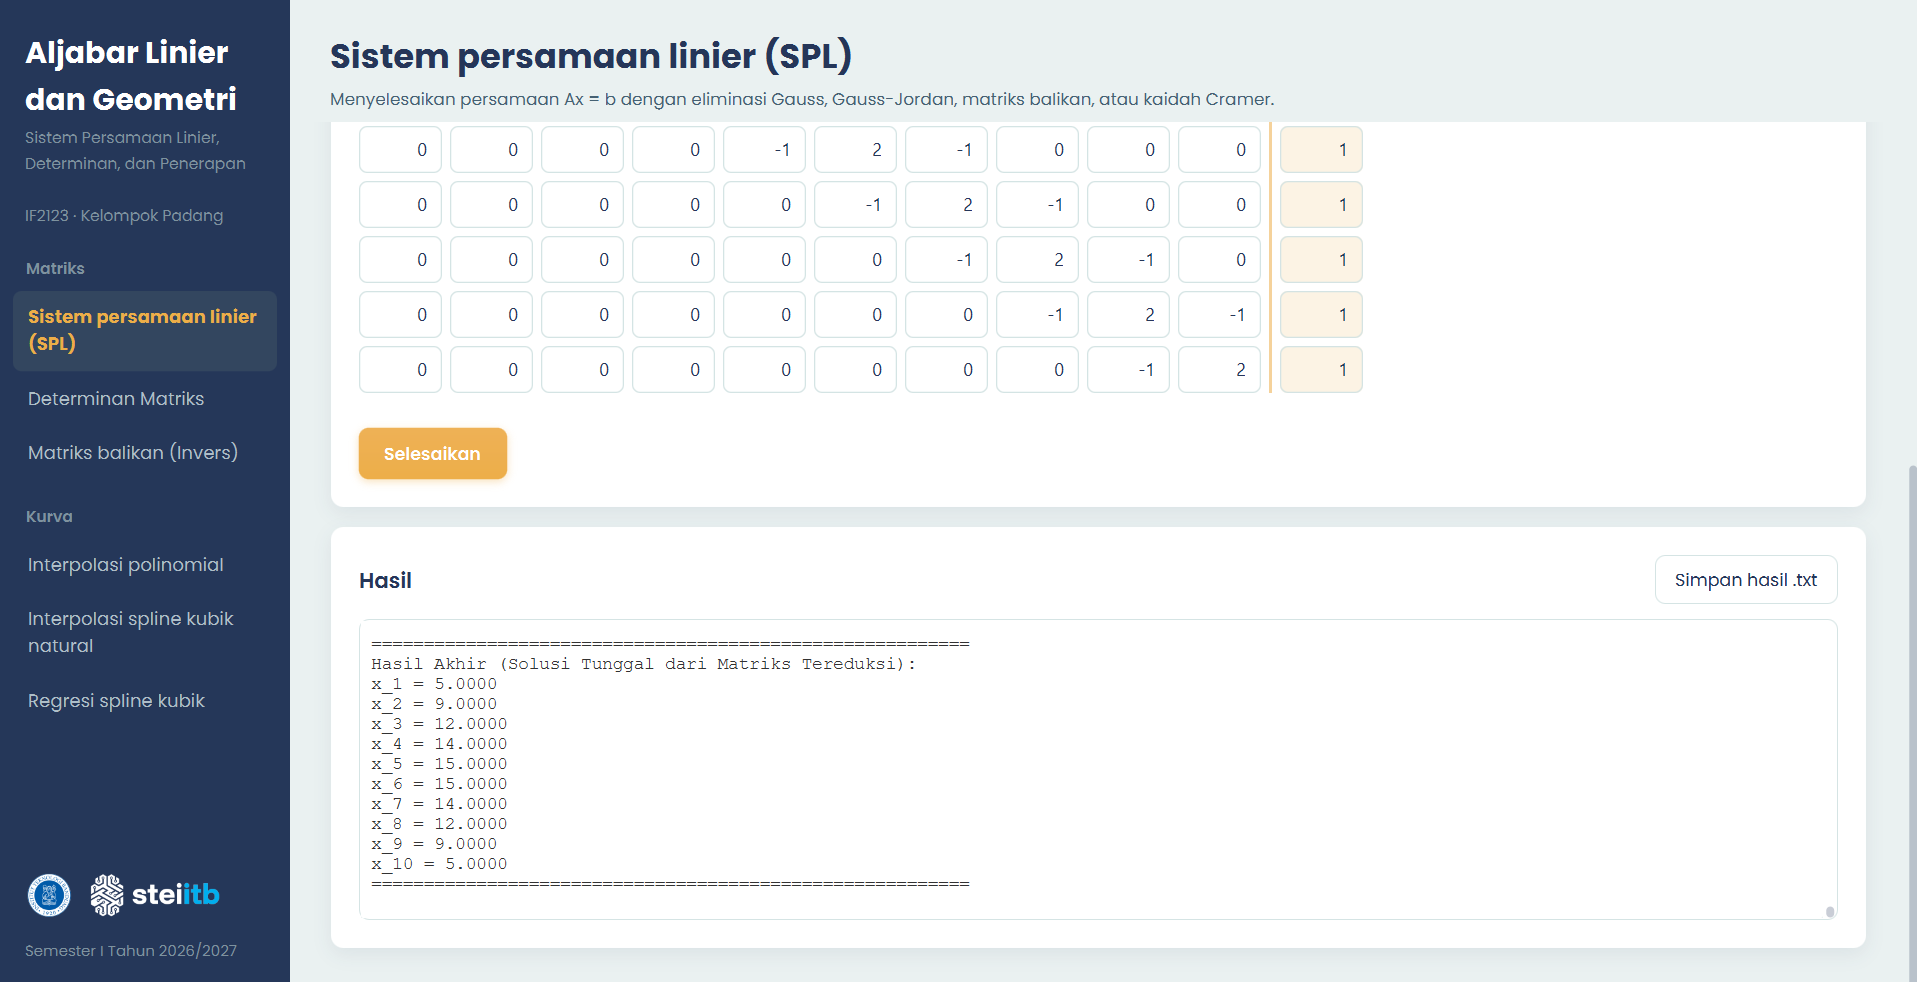
\includegraphics[width=0.8\textwidth]{5.3.4.2.gaussjordan.png}
    \caption{Penyelesaian SPL dengan Metode Gauss-Jordan}
\end{figure}
\begin{figure}[H]
    \centering
    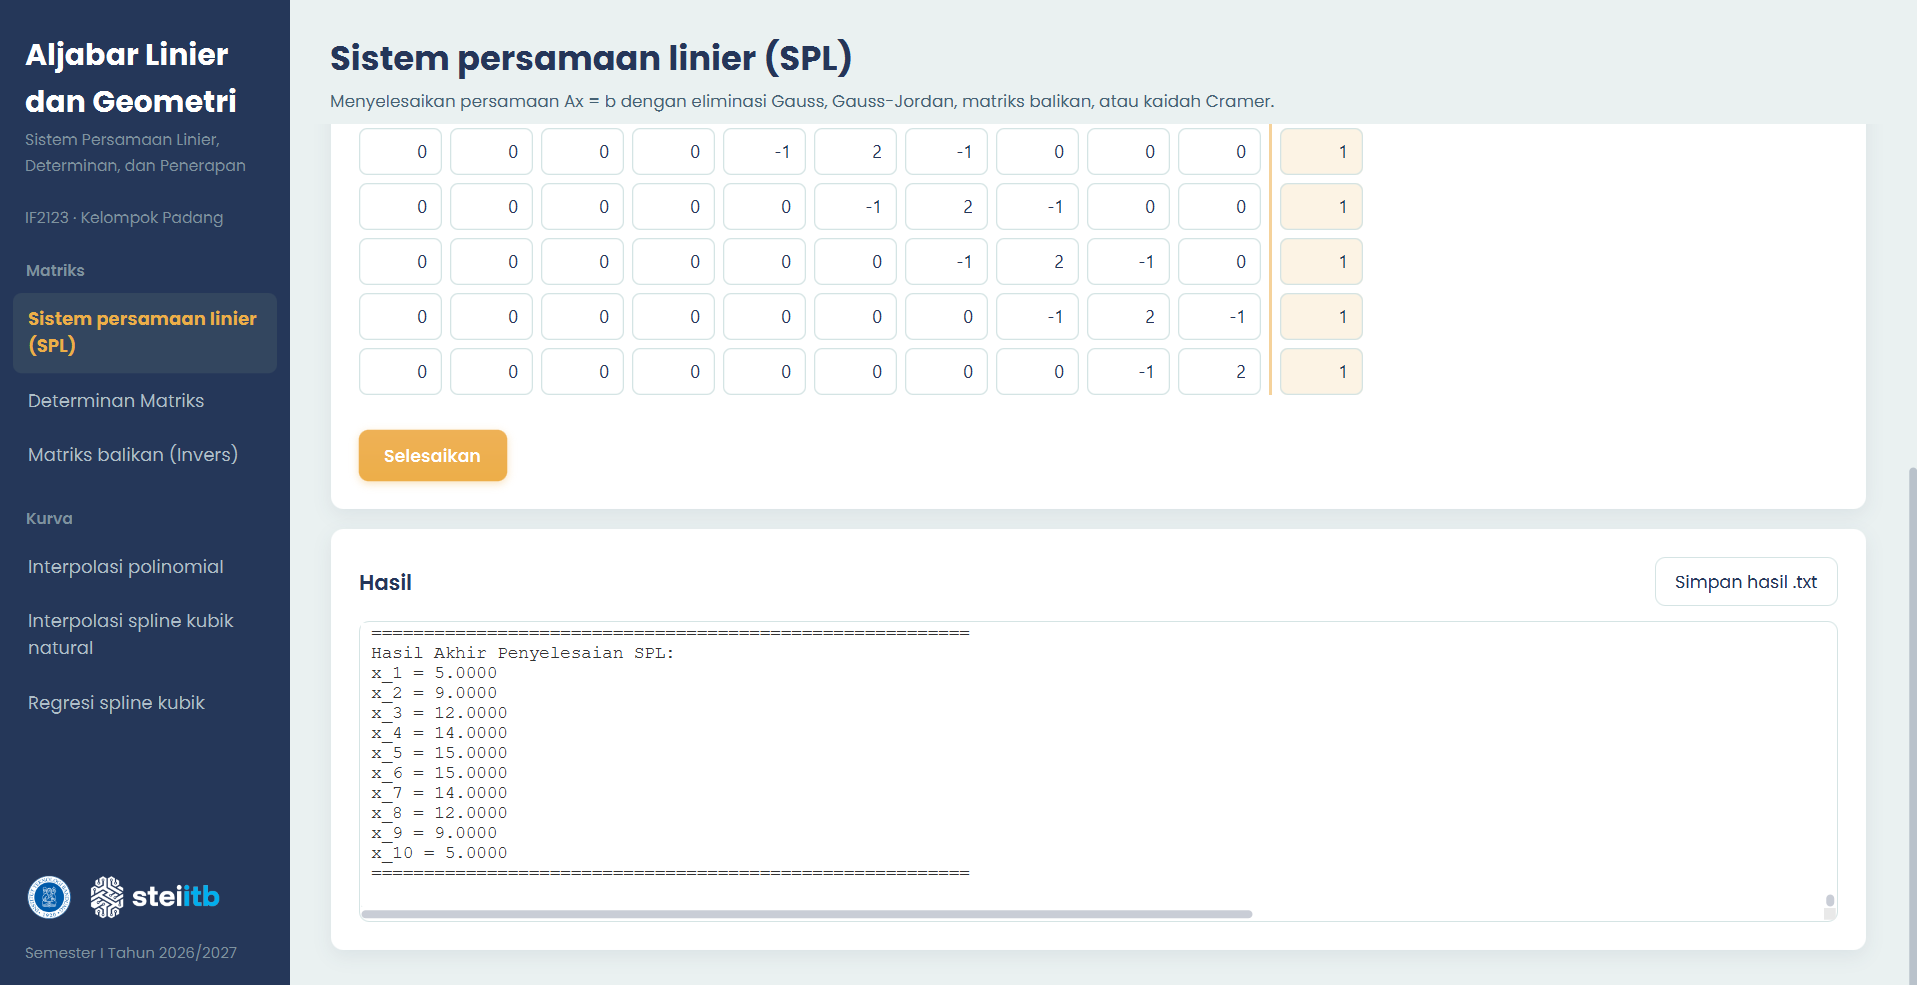
\includegraphics[width=0.8\textwidth]{5.3.4.2.invers.png}
    \caption{Penyelesaian SPL dengan Metode Invers}
\end{figure}
\begin{figure}[H]
    \centering
    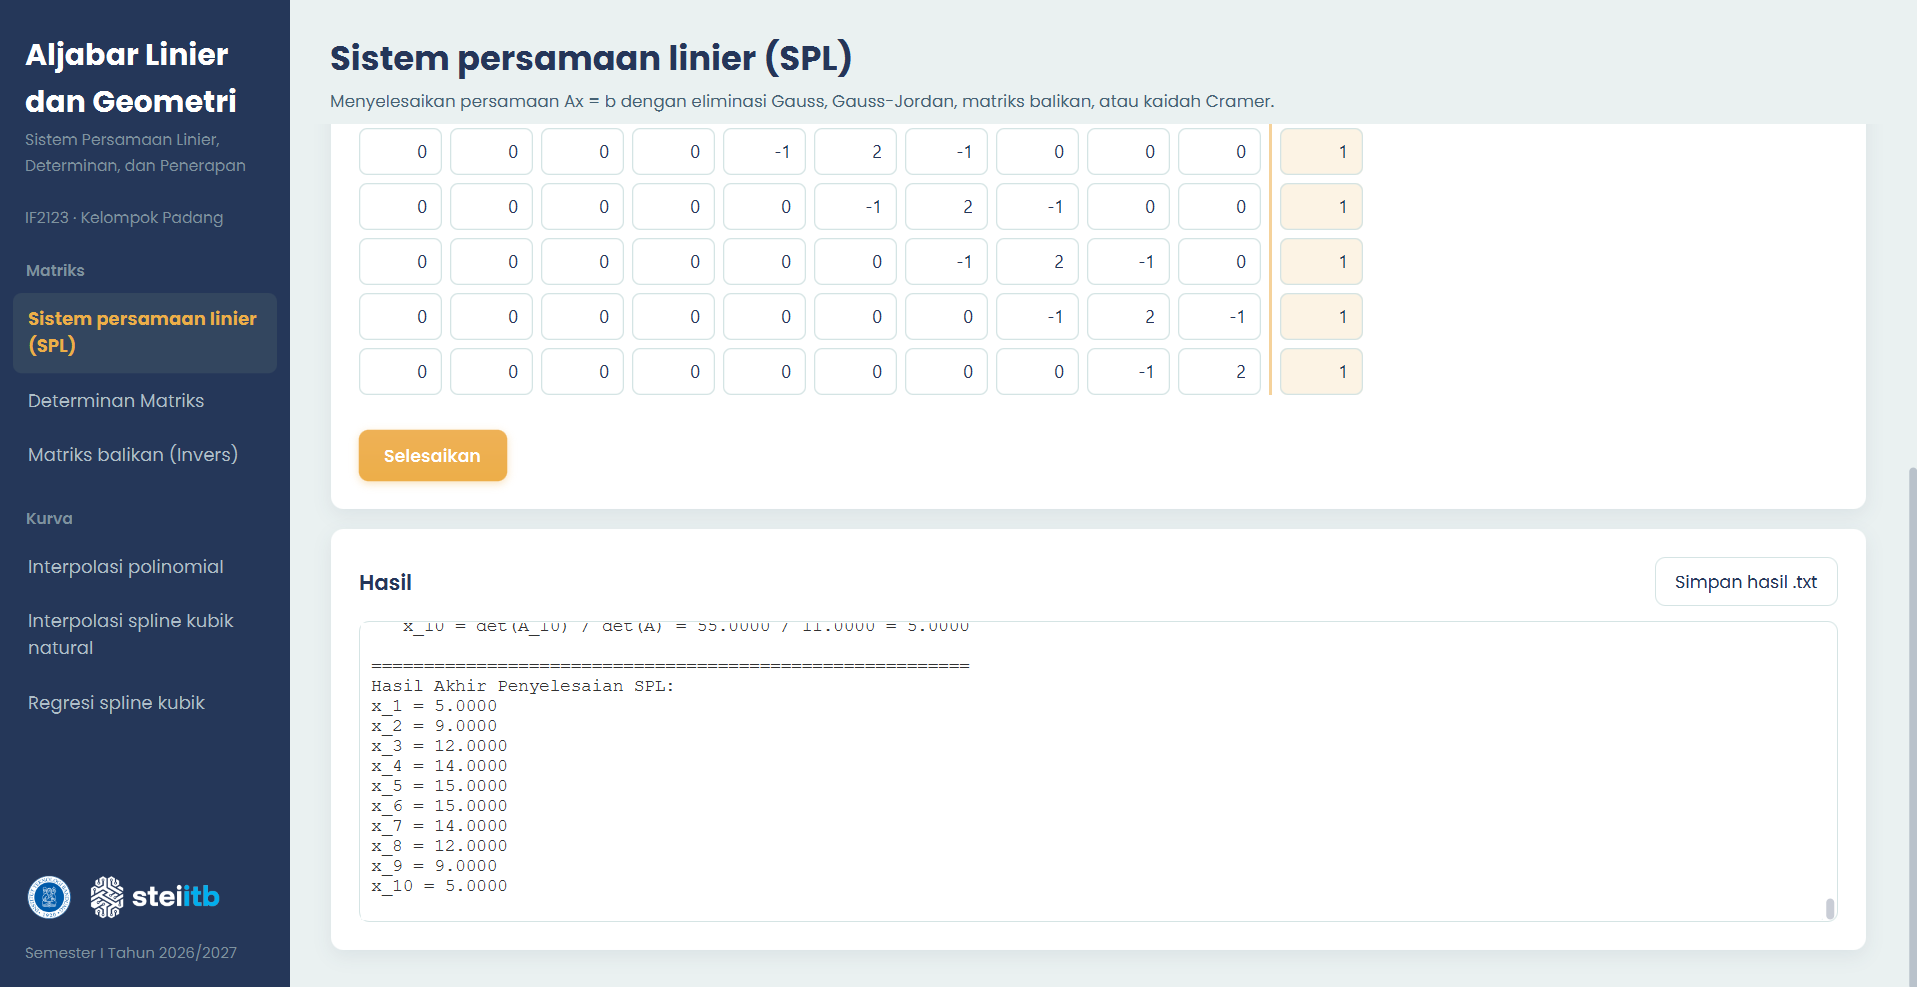
\includegraphics[width=0.8\textwidth]{5.3.4.2.cramer.png}
    \caption{Penyelesaian SPL dengan Kaidah Cramer}
\end{figure}

\textbf{Analisis:}
Seluruh metode, yaitu Eliminasi Gauss, Gauss-Jordan, Kaidah Cramer, dan Matriks Balikan, menghasilkan solusi tunggal yang konsisten. Karena determinan matriks koefisien tidak bernilai nol, matriks memiliki invers sehingga Kaidah Cramer dan Metode Matriks Balikan dapat diterapkan secara valid.

% 5.4 Sistem Persamaan Linier Berbentuk Matriks Augmented
\section{Kasus Uji 4.4: Sistem Persamaan Linier Berbentuk Matriks Augmented}

\subsection{Kasus Uji 4.4.1: Matriks augmented $A$ Berukuran $4 \times 4$}
\textbf{Matriks Masukan:}
\[
\left[ \begin{array}{cccc|c}
0 & 1 & -1 & 2 & -1 \\
2 & 0 & 1 & -1 & 3 \\
-1 & 2 & 0 & 1 & -3 \\
1 & -1 & 2 & 0 & 9
\end{array} \right]
\]

\textbf{Hasil Eksekusi Program:}
\begin{figure}[H]
    \centering
    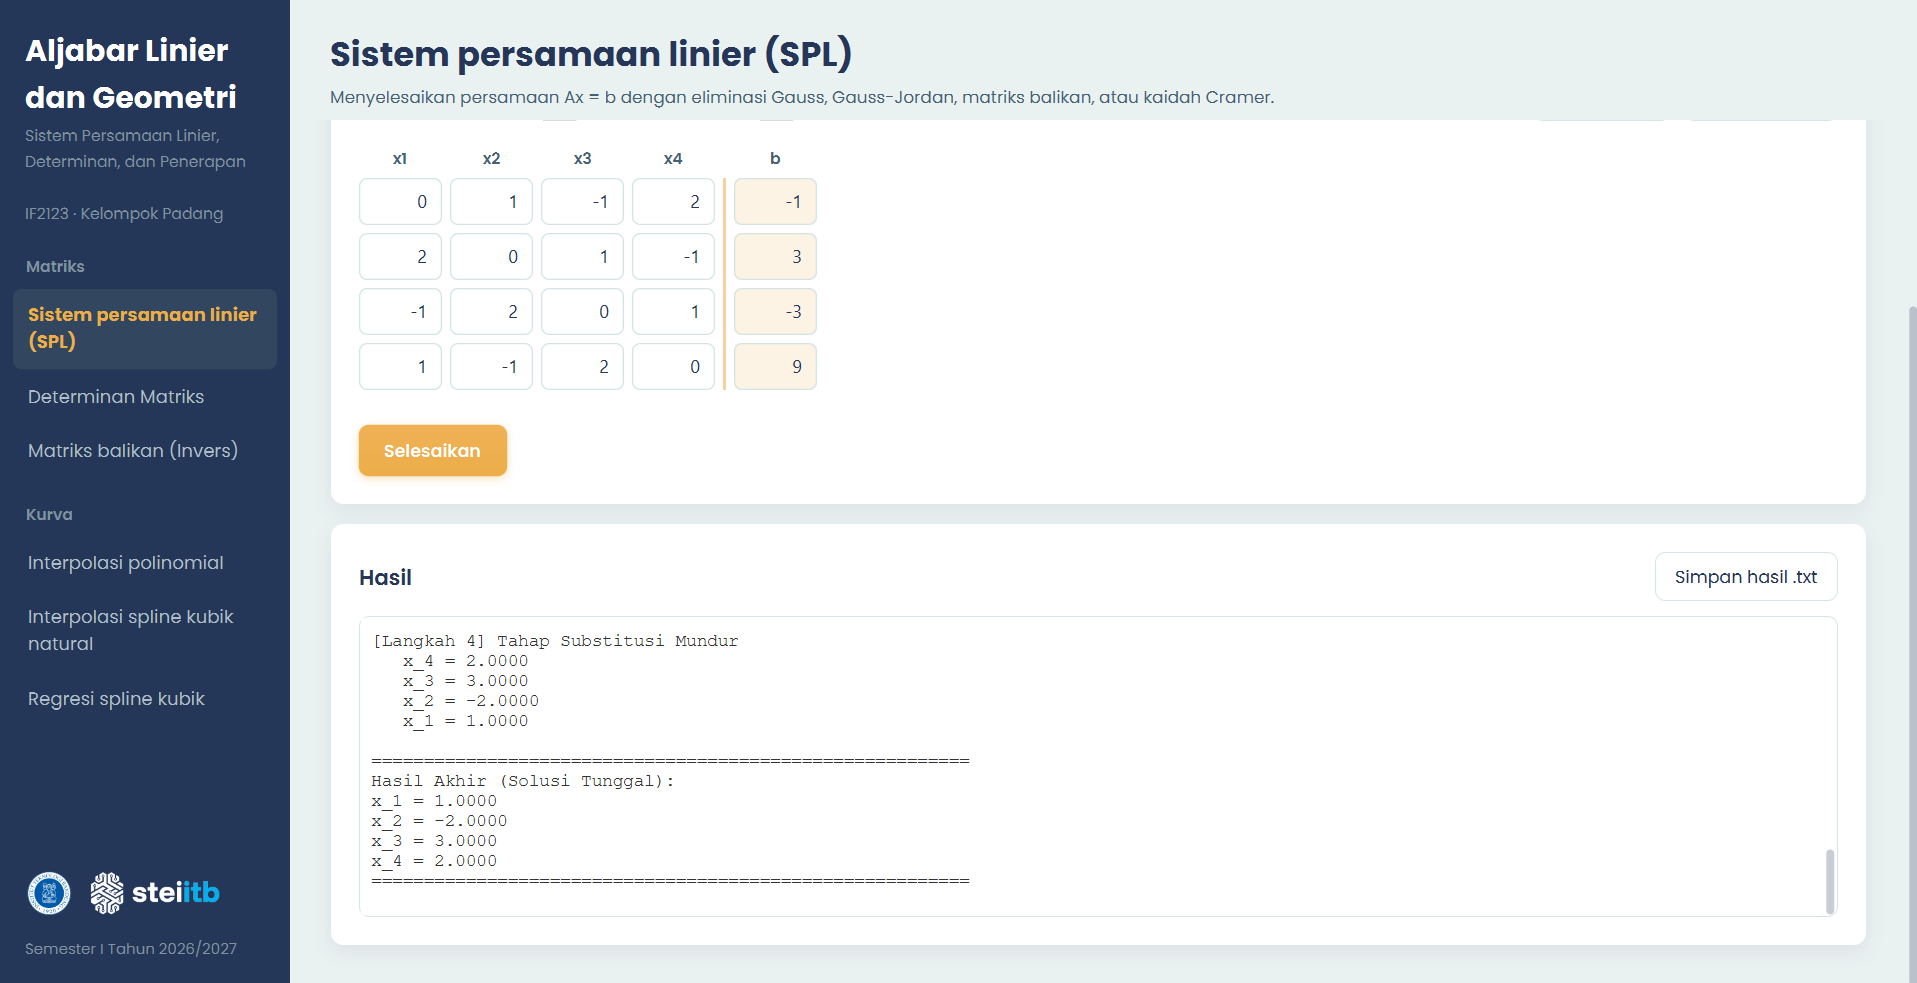
\includegraphics[width=0.8\textwidth]{5.4.1.gauss.png}
    \caption{Penyelesaian SPL dengan Metode Gauss}
\end{figure}
\begin{figure}[H]
    \centering
    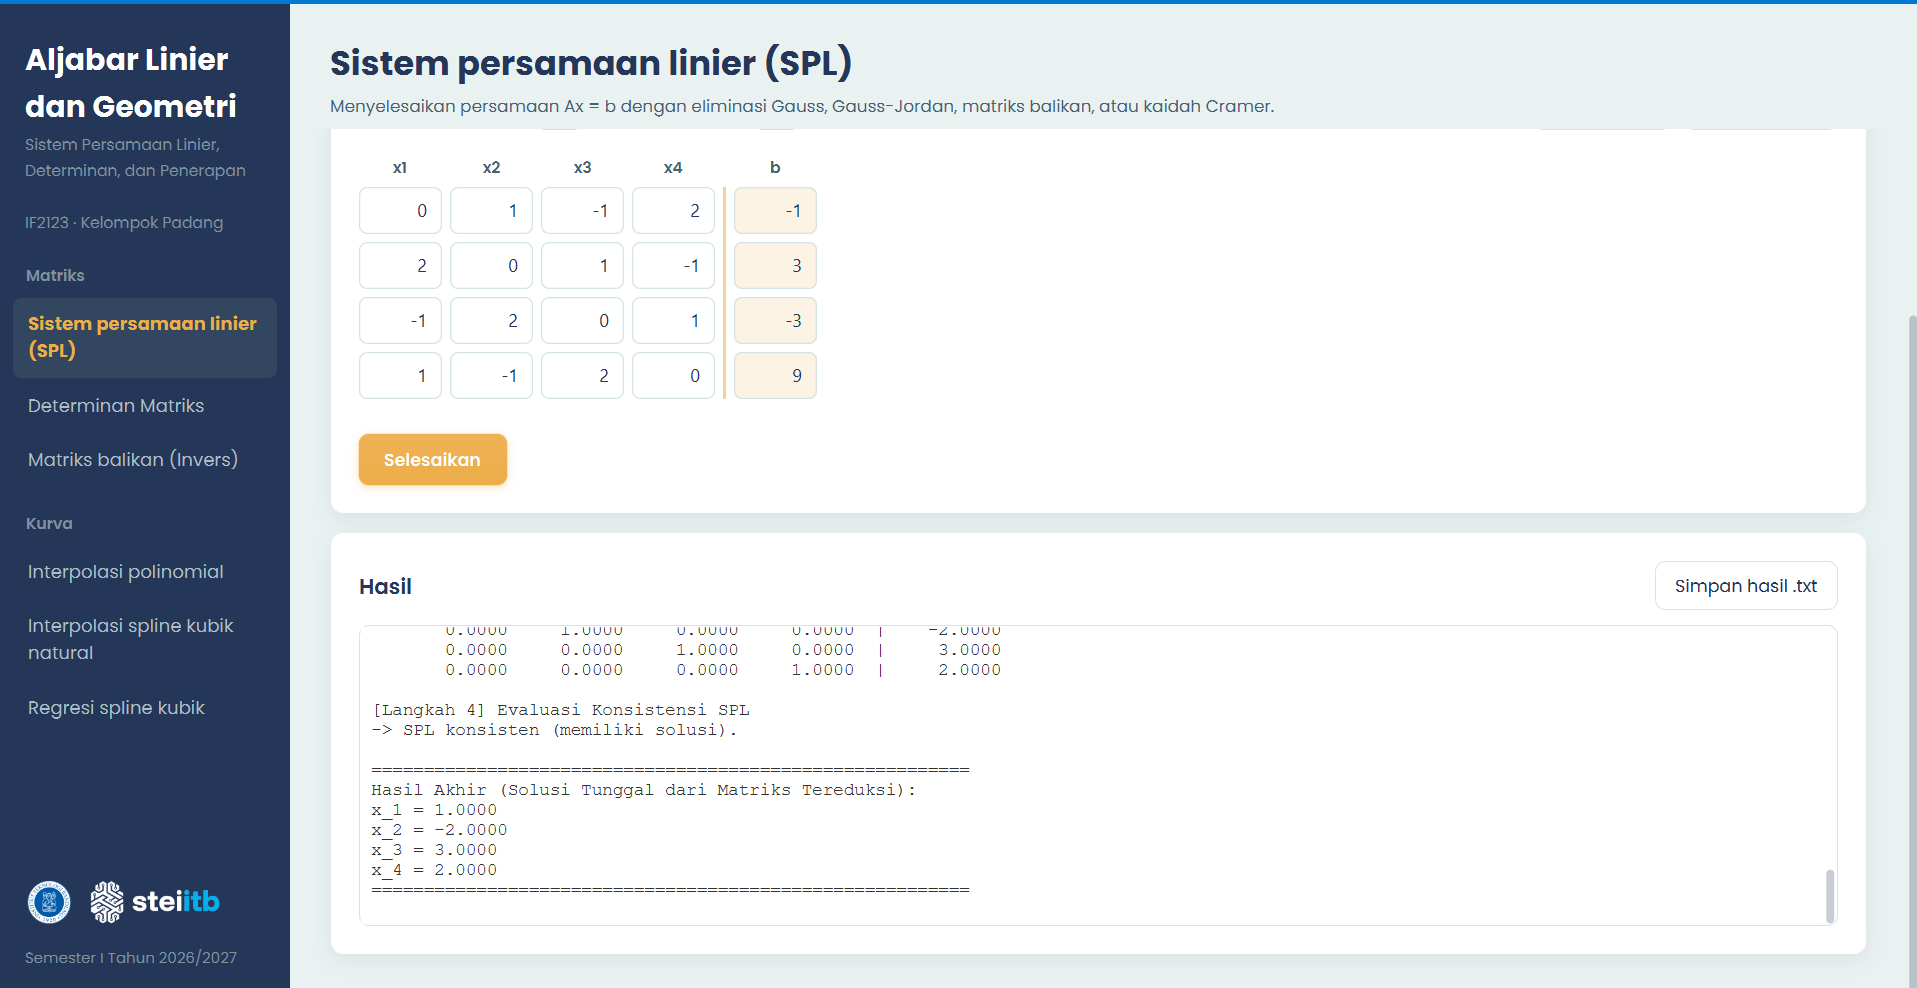
\includegraphics[width=0.8\textwidth]{5.4.1.gaussjordan.png}
    \caption{Penyelesaian SPL dengan Metode Gauss-Jordan}
\end{figure}
\begin{figure}[H]
    \centering
    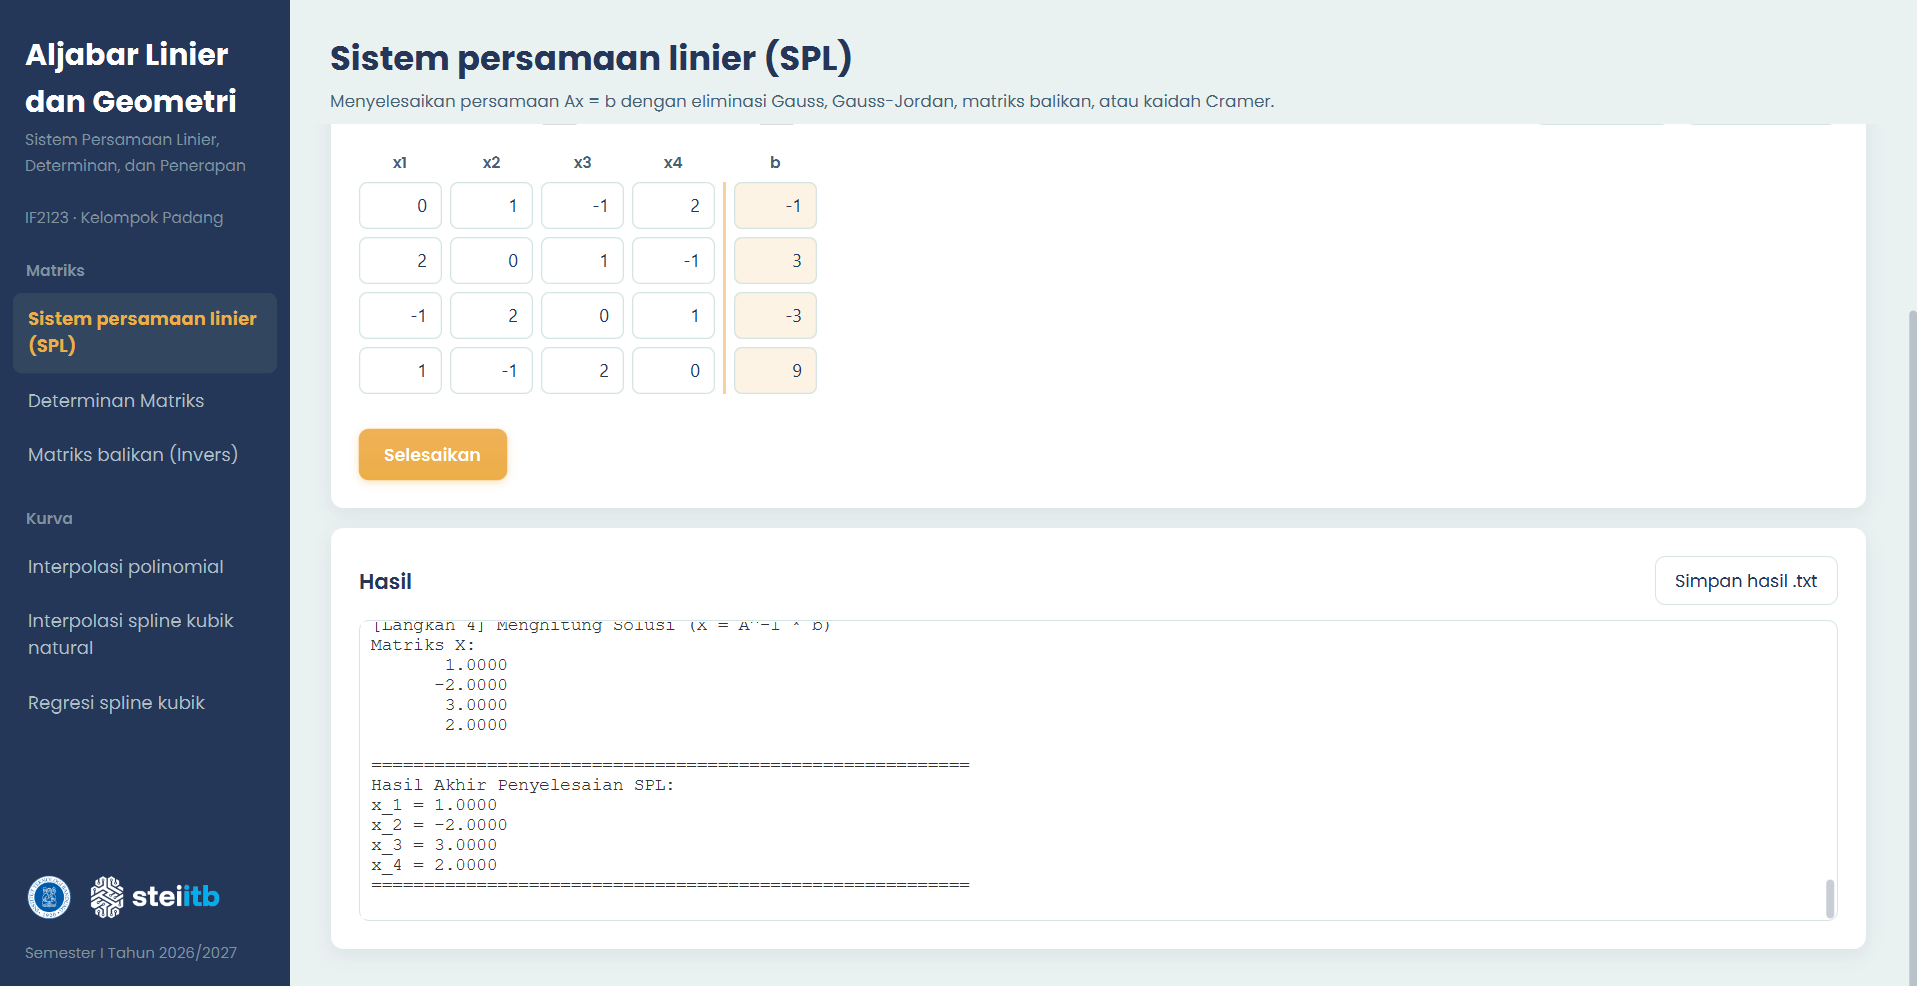
\includegraphics[width=0.8\textwidth]{5.4.1.invers.png}
    \caption{Penyelesaian SPL dengan Metode Invers}
\end{figure}
\begin{figure}[H]
    \centering
    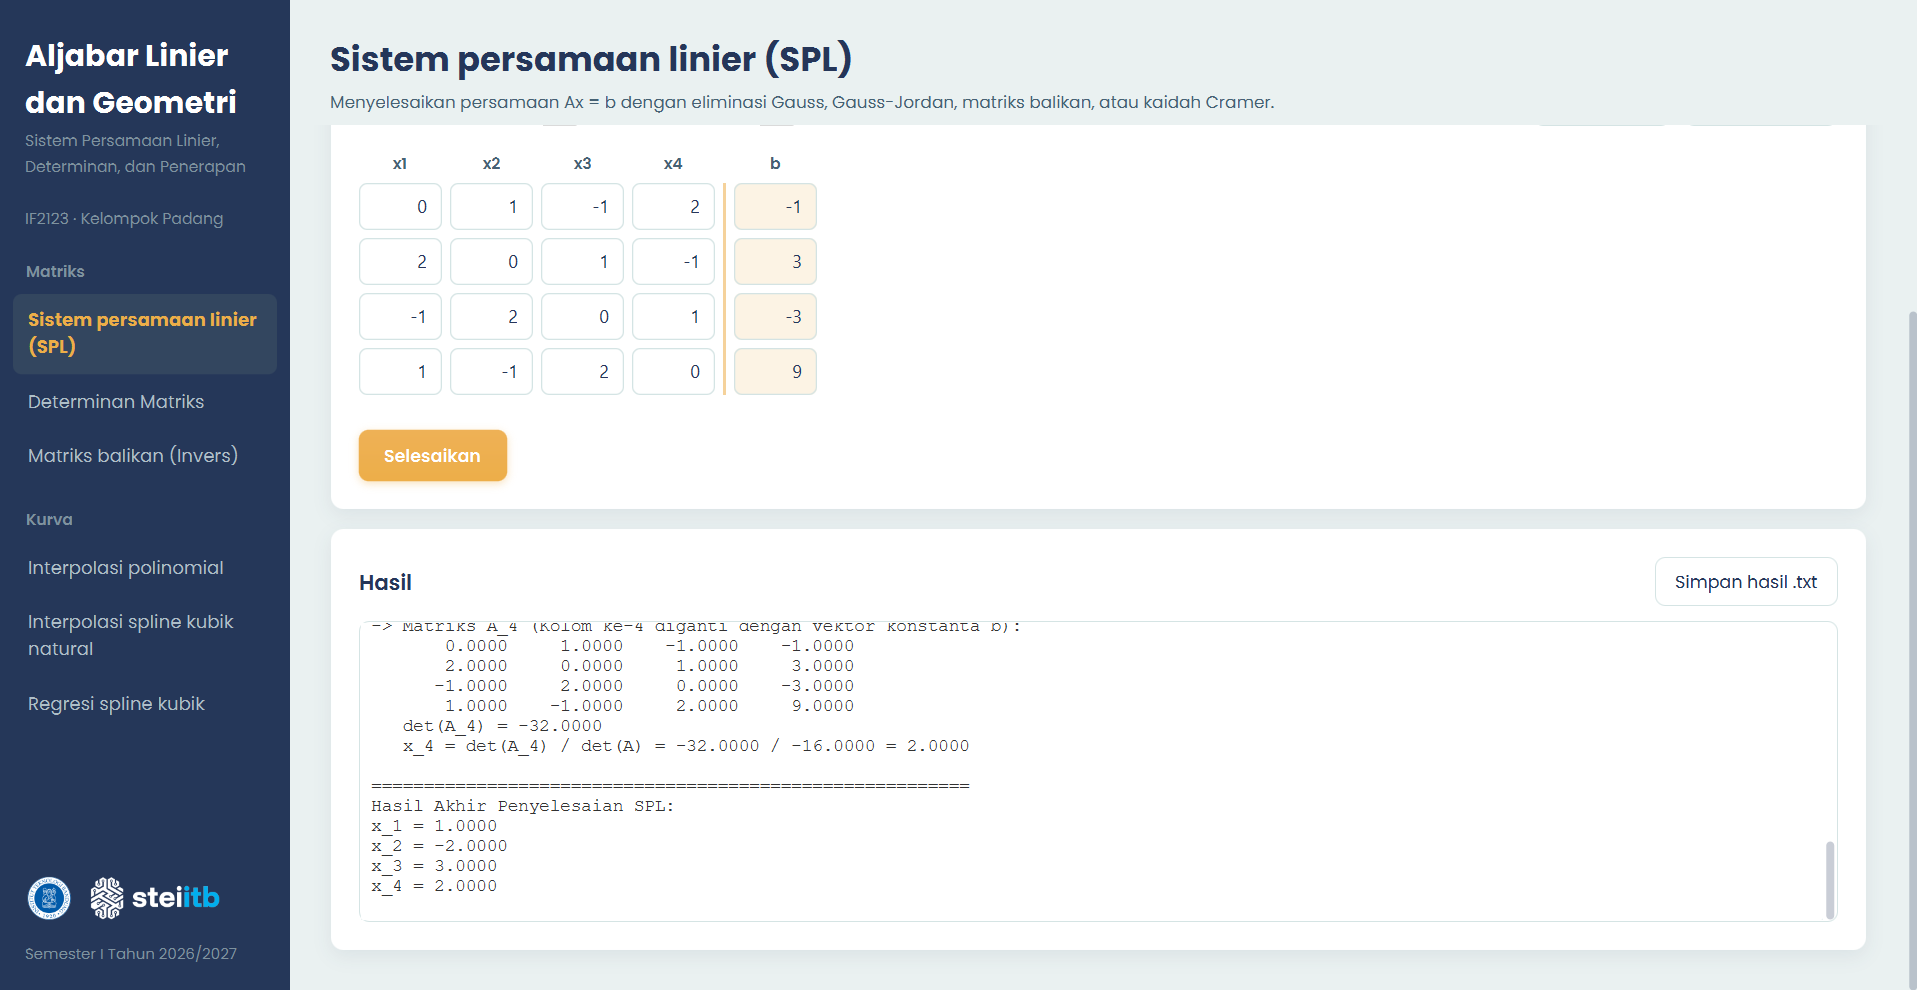
\includegraphics[width=0.8\textwidth]{5.4.1.cramer.png}
    \caption{Penyelesaian SPL dengan Kaidah Cramer}
\end{figure}

\textbf{Analisis:}
Seluruh metode, yaitu Eliminasi Gauss, Gauss-Jordan, Kaidah Cramer, dan Matriks Balikan, menghasilkan solusi tunggal yang konsisten. Karena determinan matriks koefisien tidak bernilai nol, matriks memiliki invers sehingga Kaidah Cramer dan Metode Matriks Balikan dapat diterapkan secara valid.

\subsection{Kasus Uji 4.4.2: Matriks augmented $A$ Berukuran $4 \times 6$}
\textbf{Matriks Masukan:}
\[
\left[ \begin{array}{cccccc|c}
1 & 0 & 2 & -1 & 0 & 3 & -7 \\
0 & 1 & -1 & 2 & 1 & 0 & 6 \\
2 & -1 & 0 & 1 & 3 & -2 & 13 \\
1 & 1 & 1 & 1 & 1 & 1 & 3
\end{array} \right]
\]

\textbf{Hasil Eksekusi Program:}
\begin{figure}[H]
    \centering
    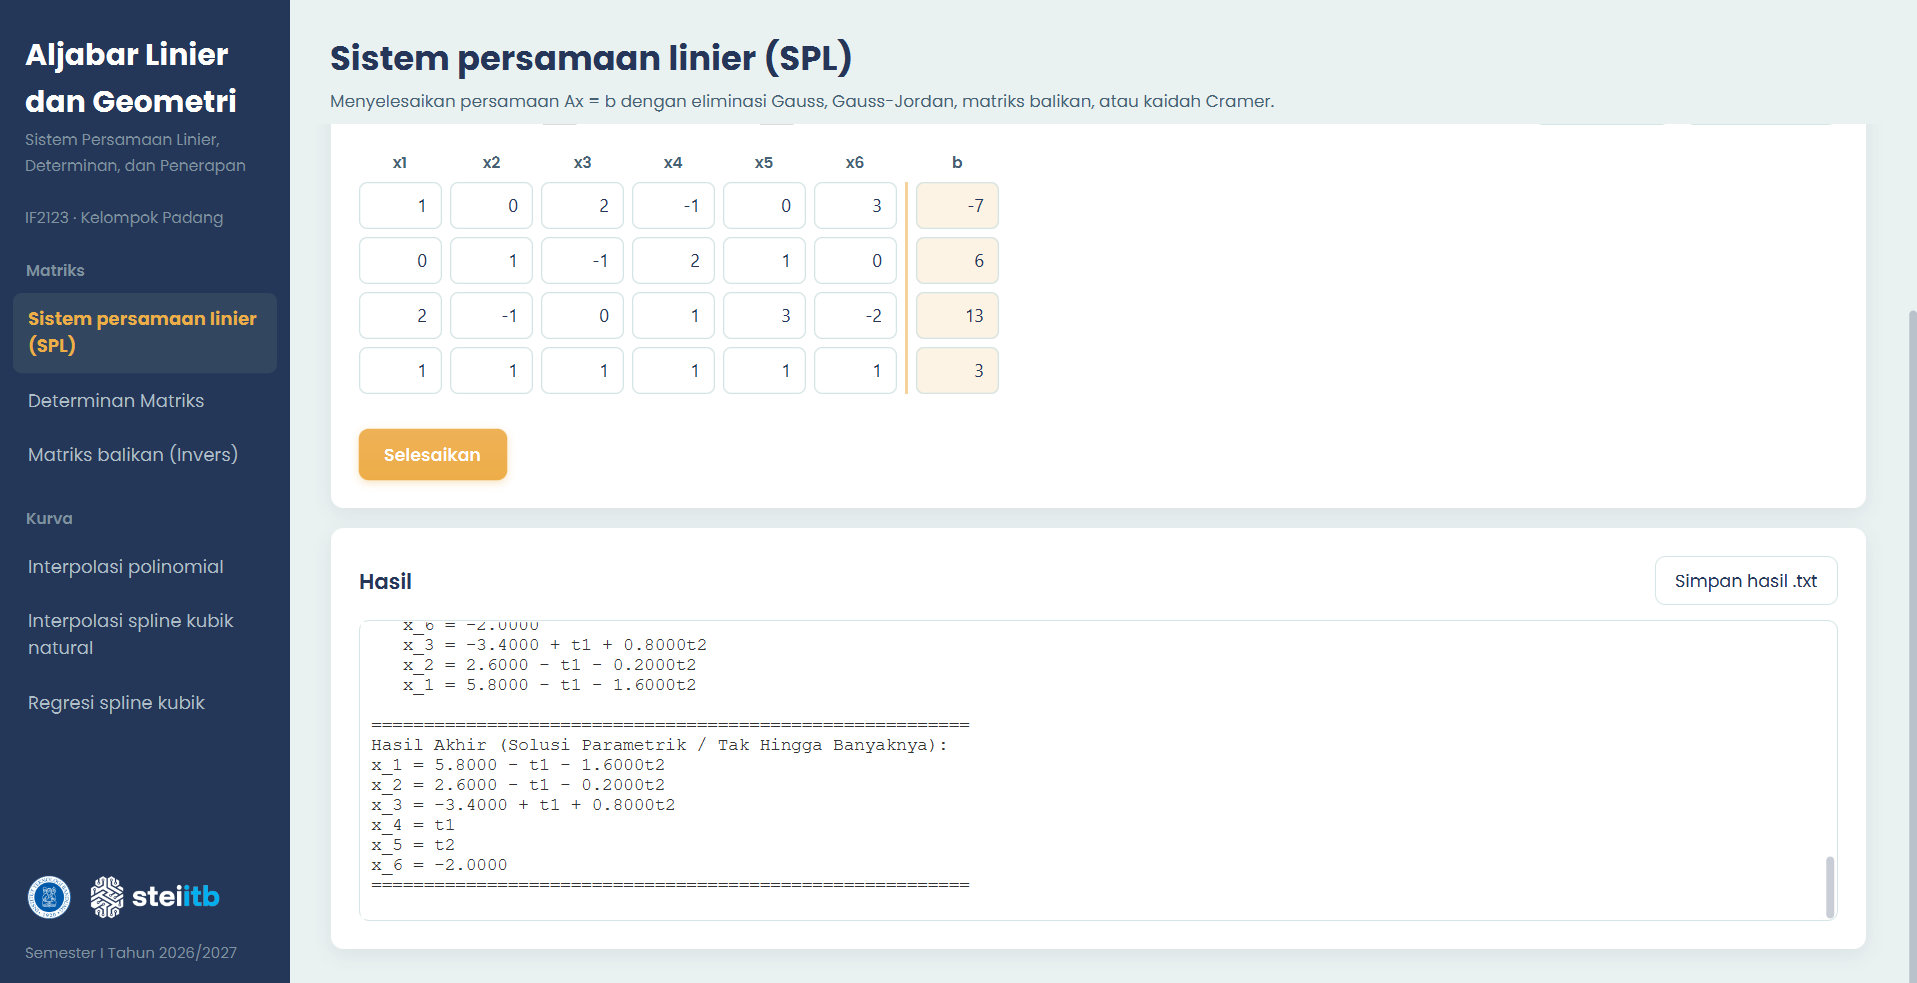
\includegraphics[width=0.8\textwidth]{5.4.2.gauss.png}
    \caption{Penyelesaian SPL dengan Metode Gauss}
\end{figure}
\begin{figure}[H]
    \centering
    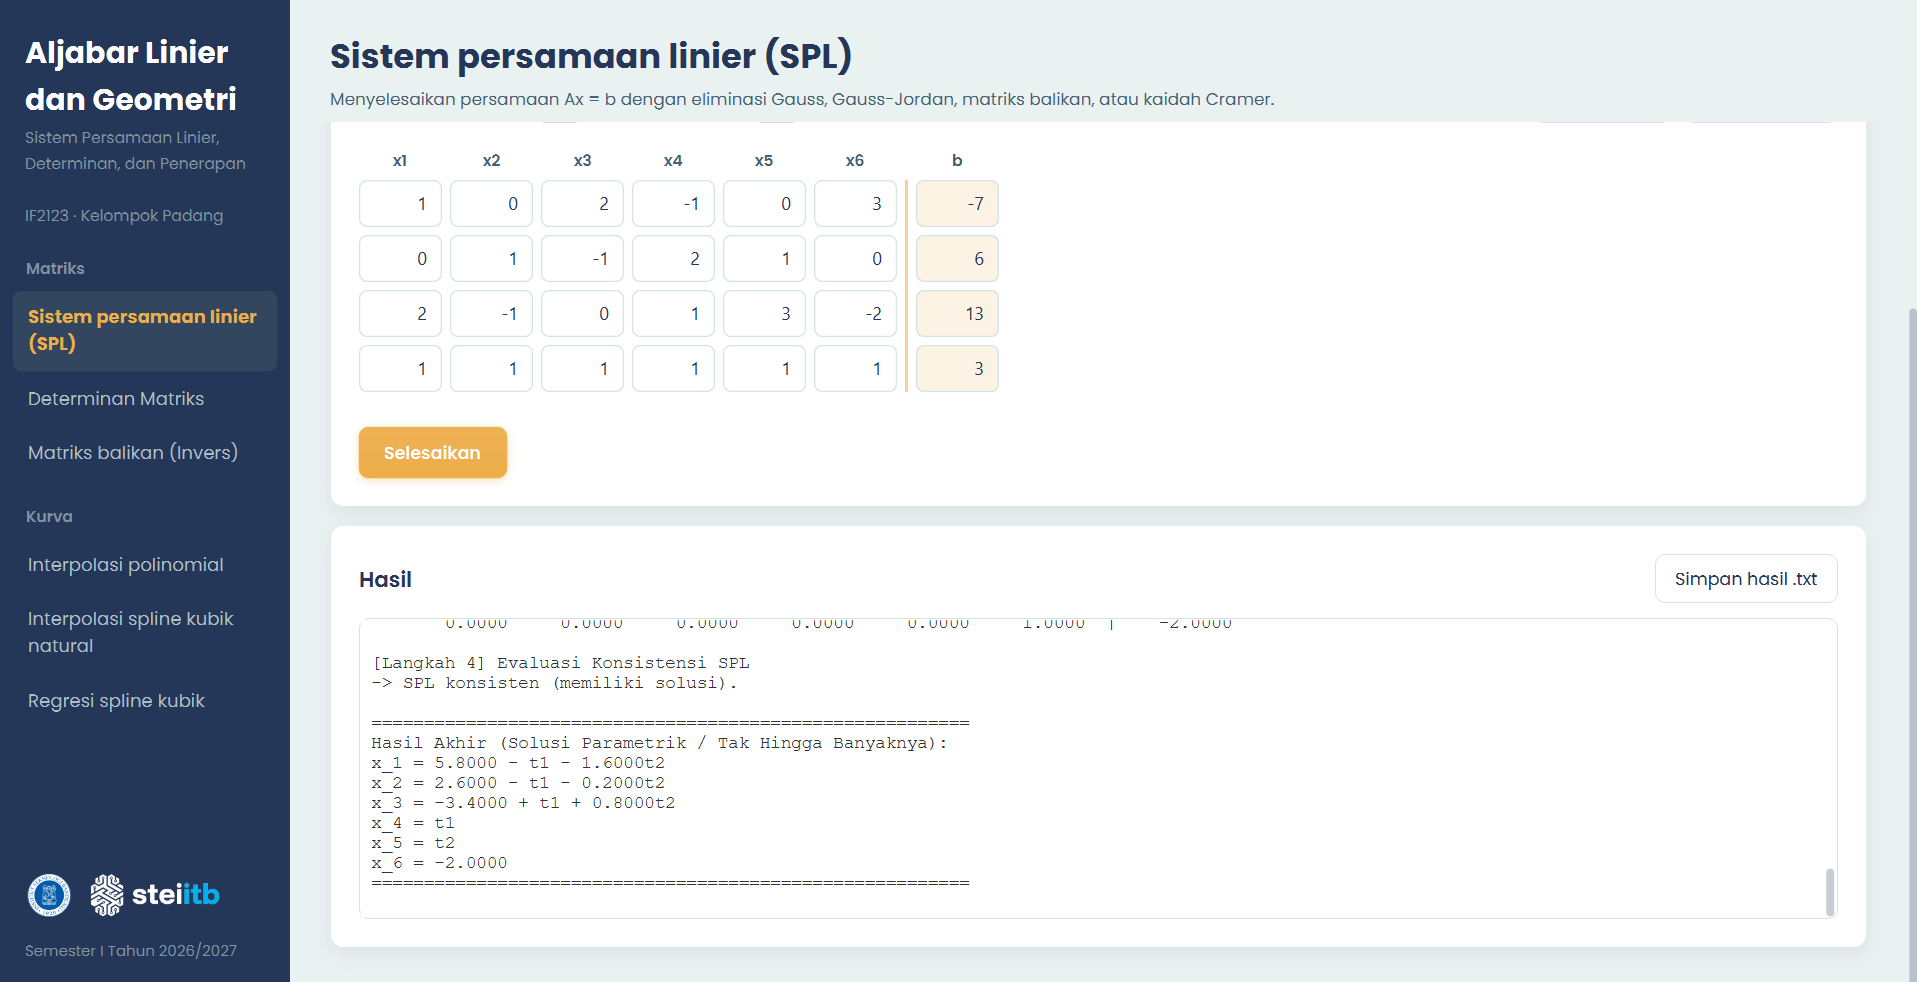
\includegraphics[width=0.8\textwidth]{5.4.2.gaussjordan.png}
    \caption{Penyelesaian SPL dengan Metode Gauss-Jordan}
\end{figure}
\begin{figure}[H]
    \centering
    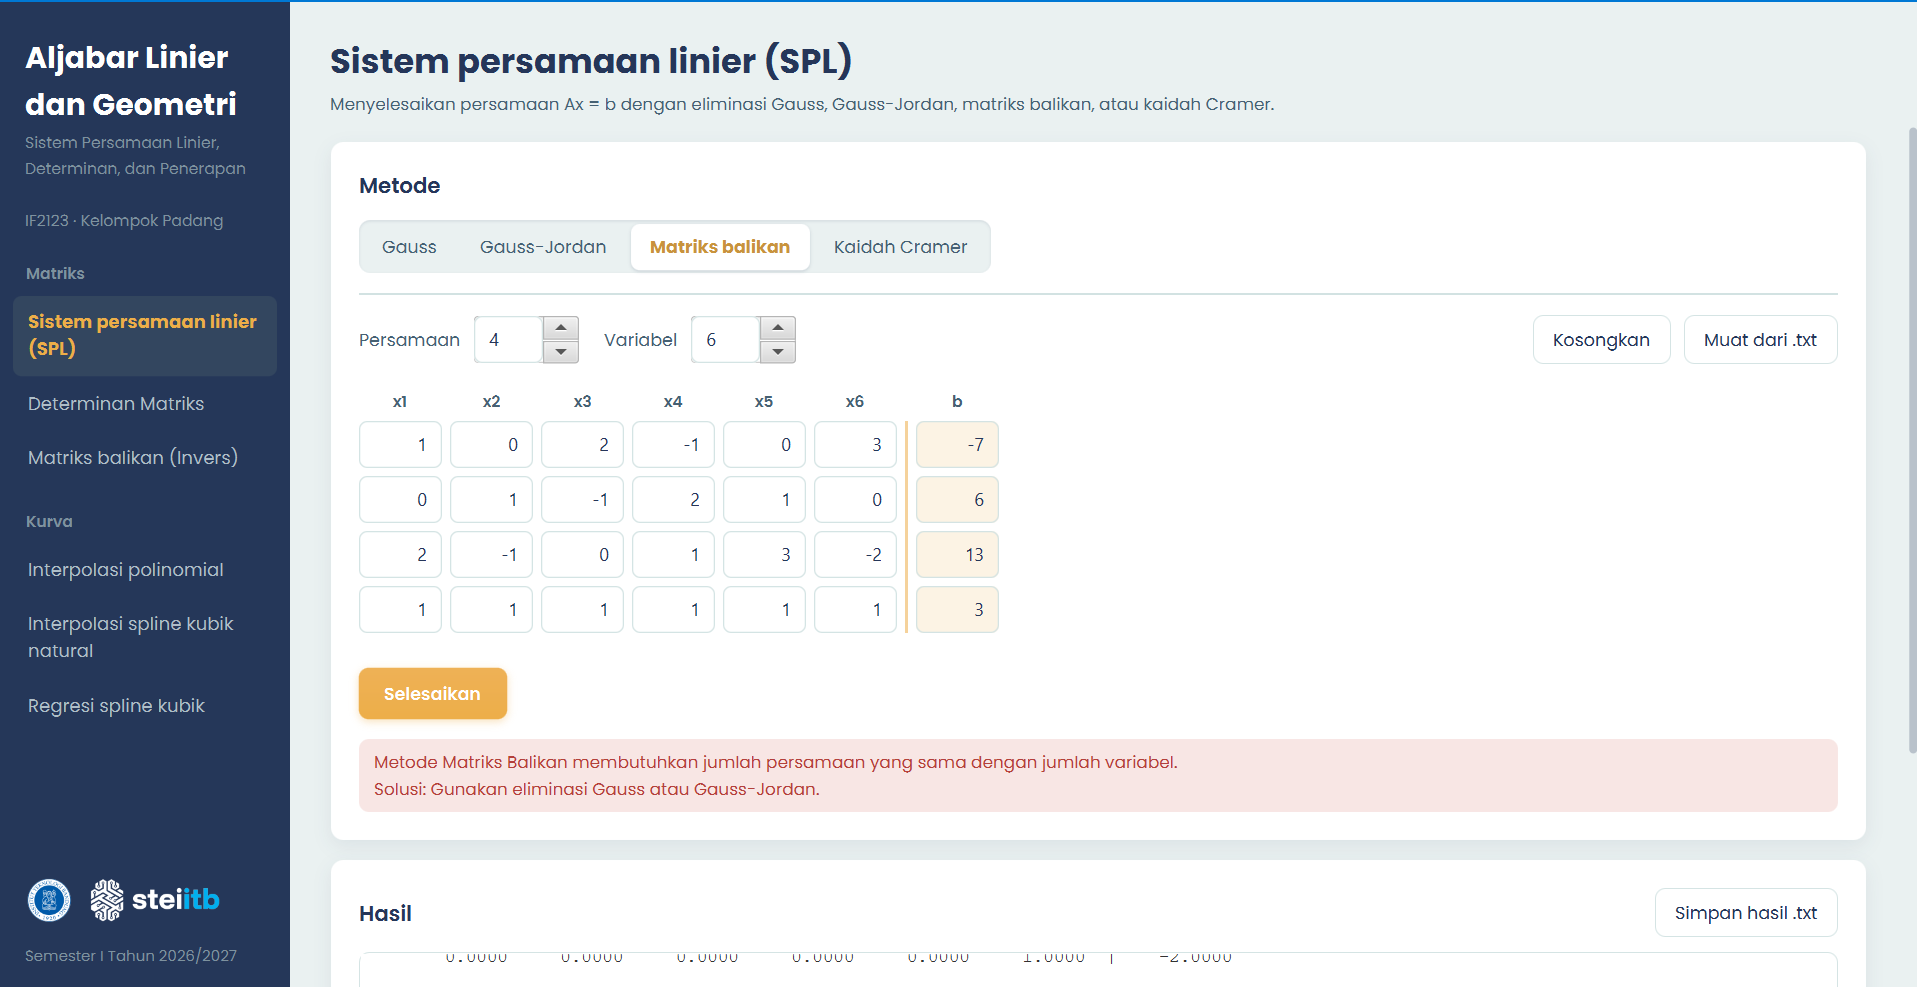
\includegraphics[width=0.8\textwidth]{5.4.2.invers.png}
    \caption{Penyelesaian SPL dengan Metode Invers}
\end{figure}
\begin{figure}[H]
    \centering
    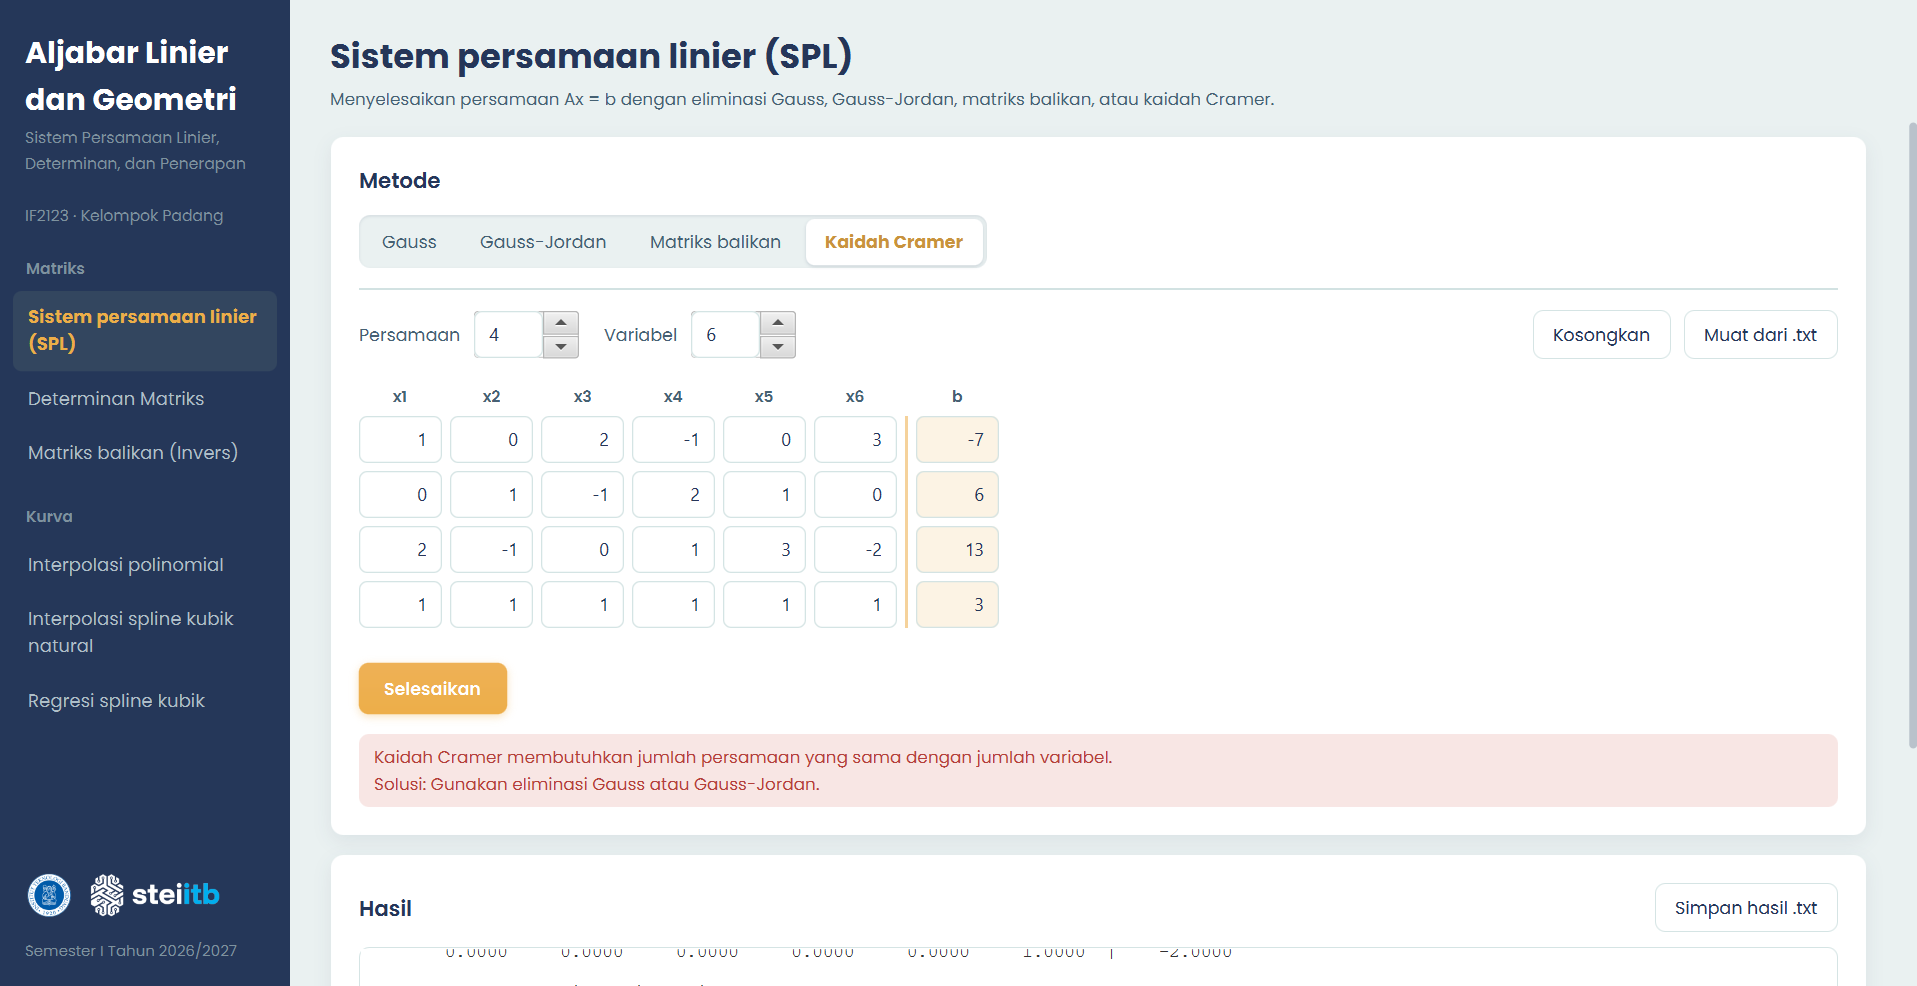
\includegraphics[width=0.8\textwidth]{5.4.2.cramer.png}
    \caption{Penyelesaian SPL dengan Kaidah Cramer}
\end{figure}

\textbf{Analisis:}
Matriks memiliki jumlah variabel yang lebih banyak daripada persamaan tidak memenuhi syarat Kaidah Cramer dan Metode Matriks Balikan sehingga metode yang dapat digunakan hanya metode Eliminasi Gauss dan Gauss-Jordan.


% 5.5 Sistem Persamaan Linier Berbentuk Umum
\section{Kasus Uji 4.5: Sistem Persamaan Linier Berbentuk Umum}

\subsection{Kasus Uji 4.5.1: SPL $4 \times 4$ }
\textbf{Sistem Persamaan Masukan:}
\begin{align*}
3x_1 + 2x_2 - x_3 + 4x_4 &= 5 \\
x_1 - 3x_2 + 2x_3 + x_4 &= -2 \\
4x_1 + x_2 + 5x_3 - 2x_4 &= 7 \\
2x_1 - x_2 + 3x_3 + x_4 &= 3
\end{align*}

\textbf{Hasil Eksekusi Program:}
\begin{figure}[H]
    \centering
    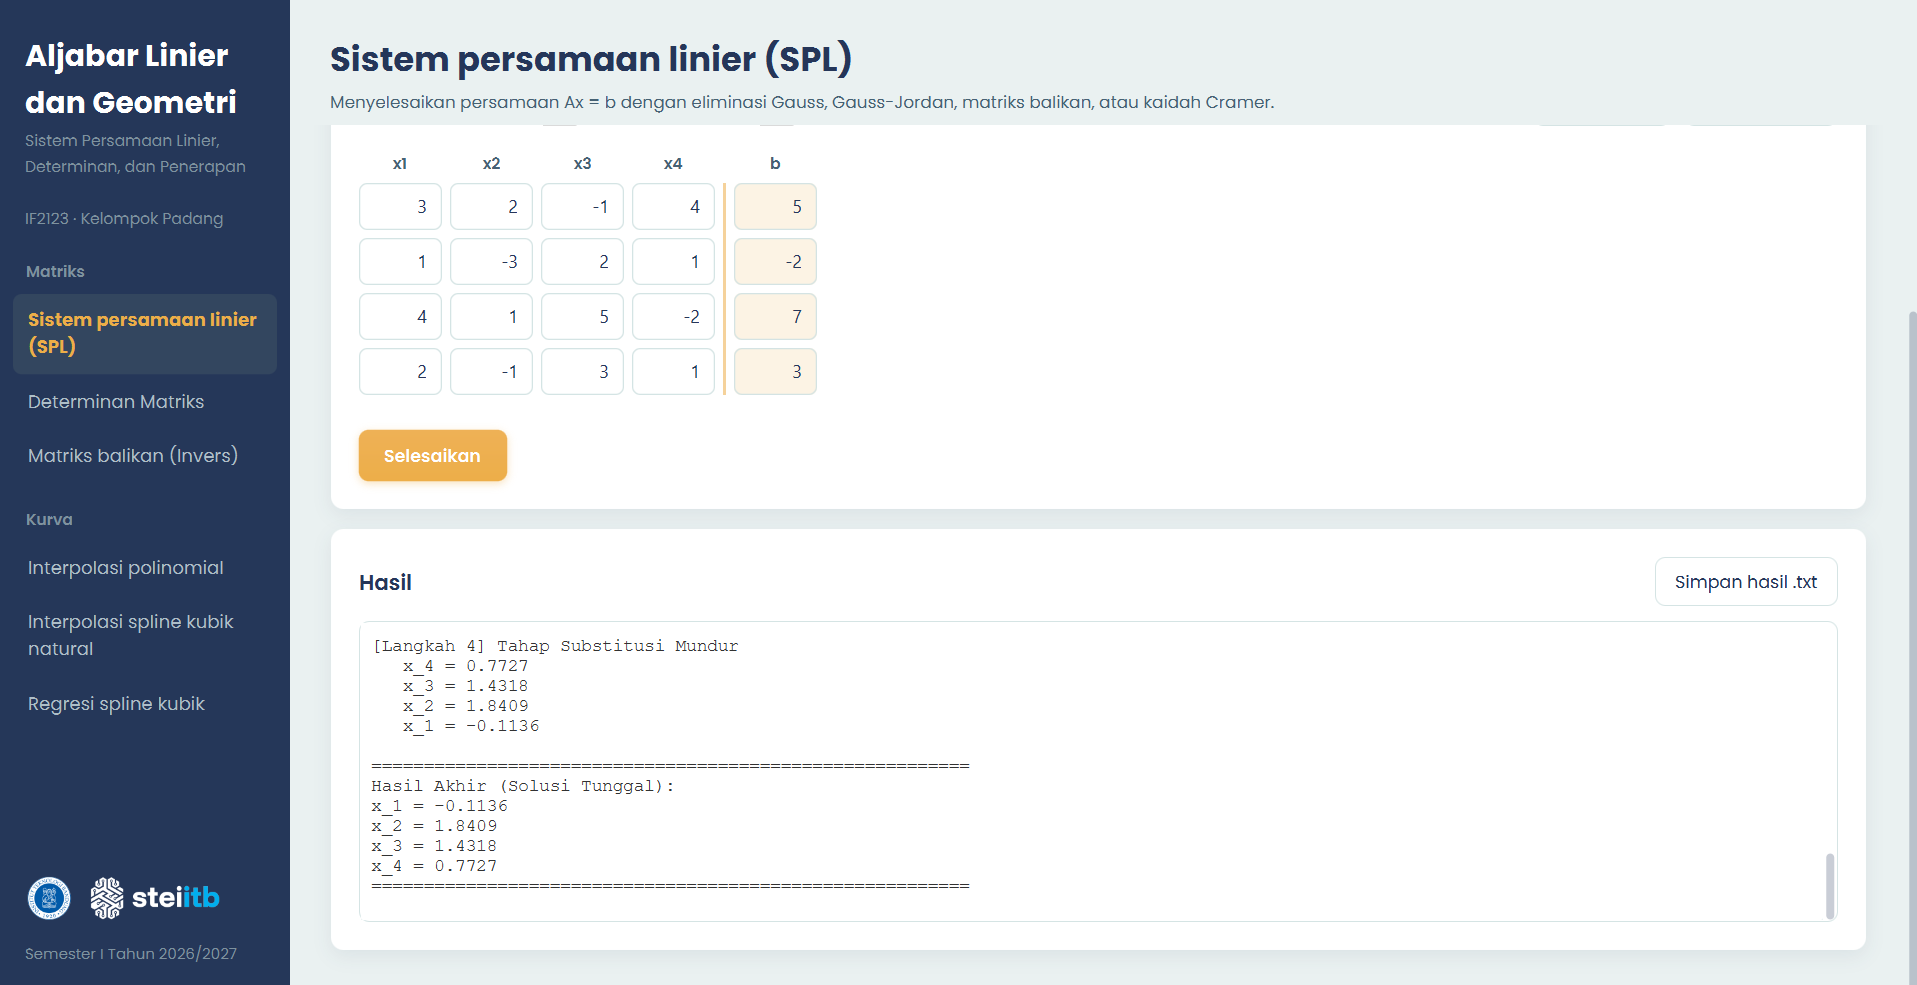
\includegraphics[width=0.8\textwidth]{5.5.1.gauss.png}
    \caption{Penyelesaian SPL dengan Metode Gauss}
\end{figure}
\begin{figure}[H]
    \centering
    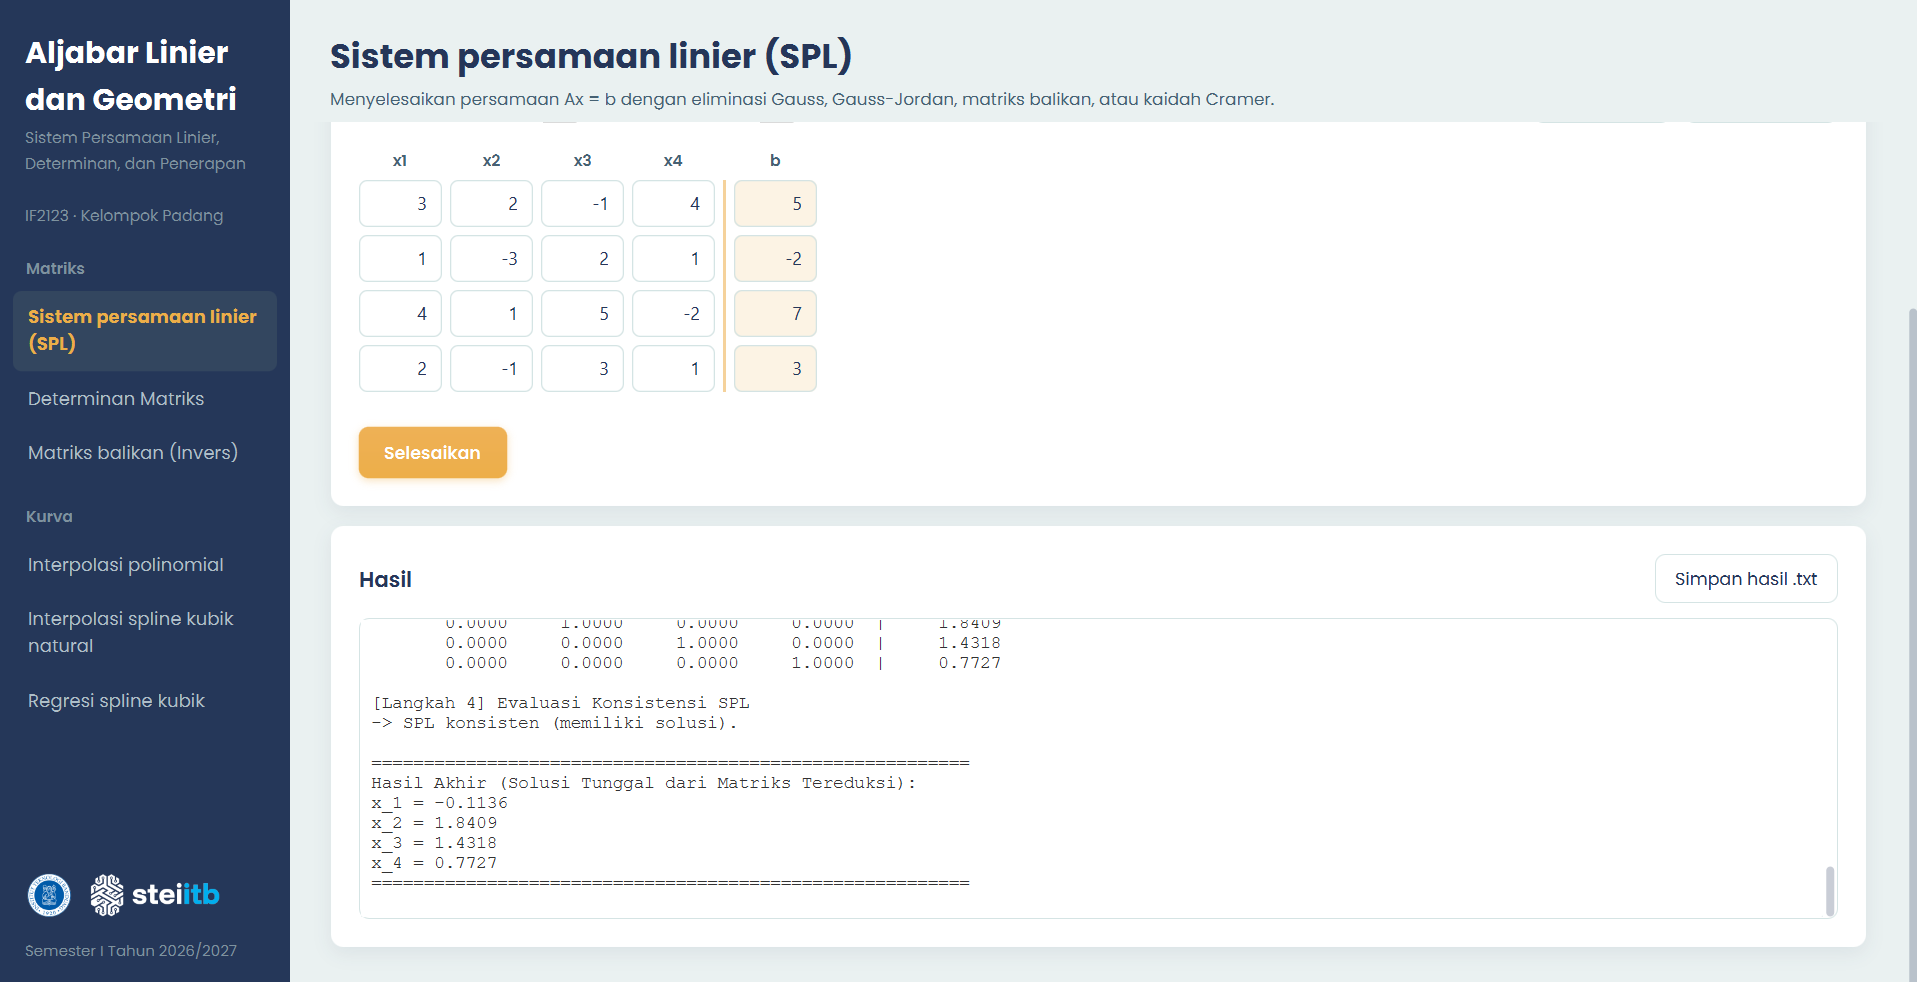
\includegraphics[width=0.8\textwidth]{5.5.1.gaussjordan.png}
    \caption{Penyelesaian SPL dengan Metode Gauss-Jordan}
\end{figure}
\begin{figure}[H]
    \centering
    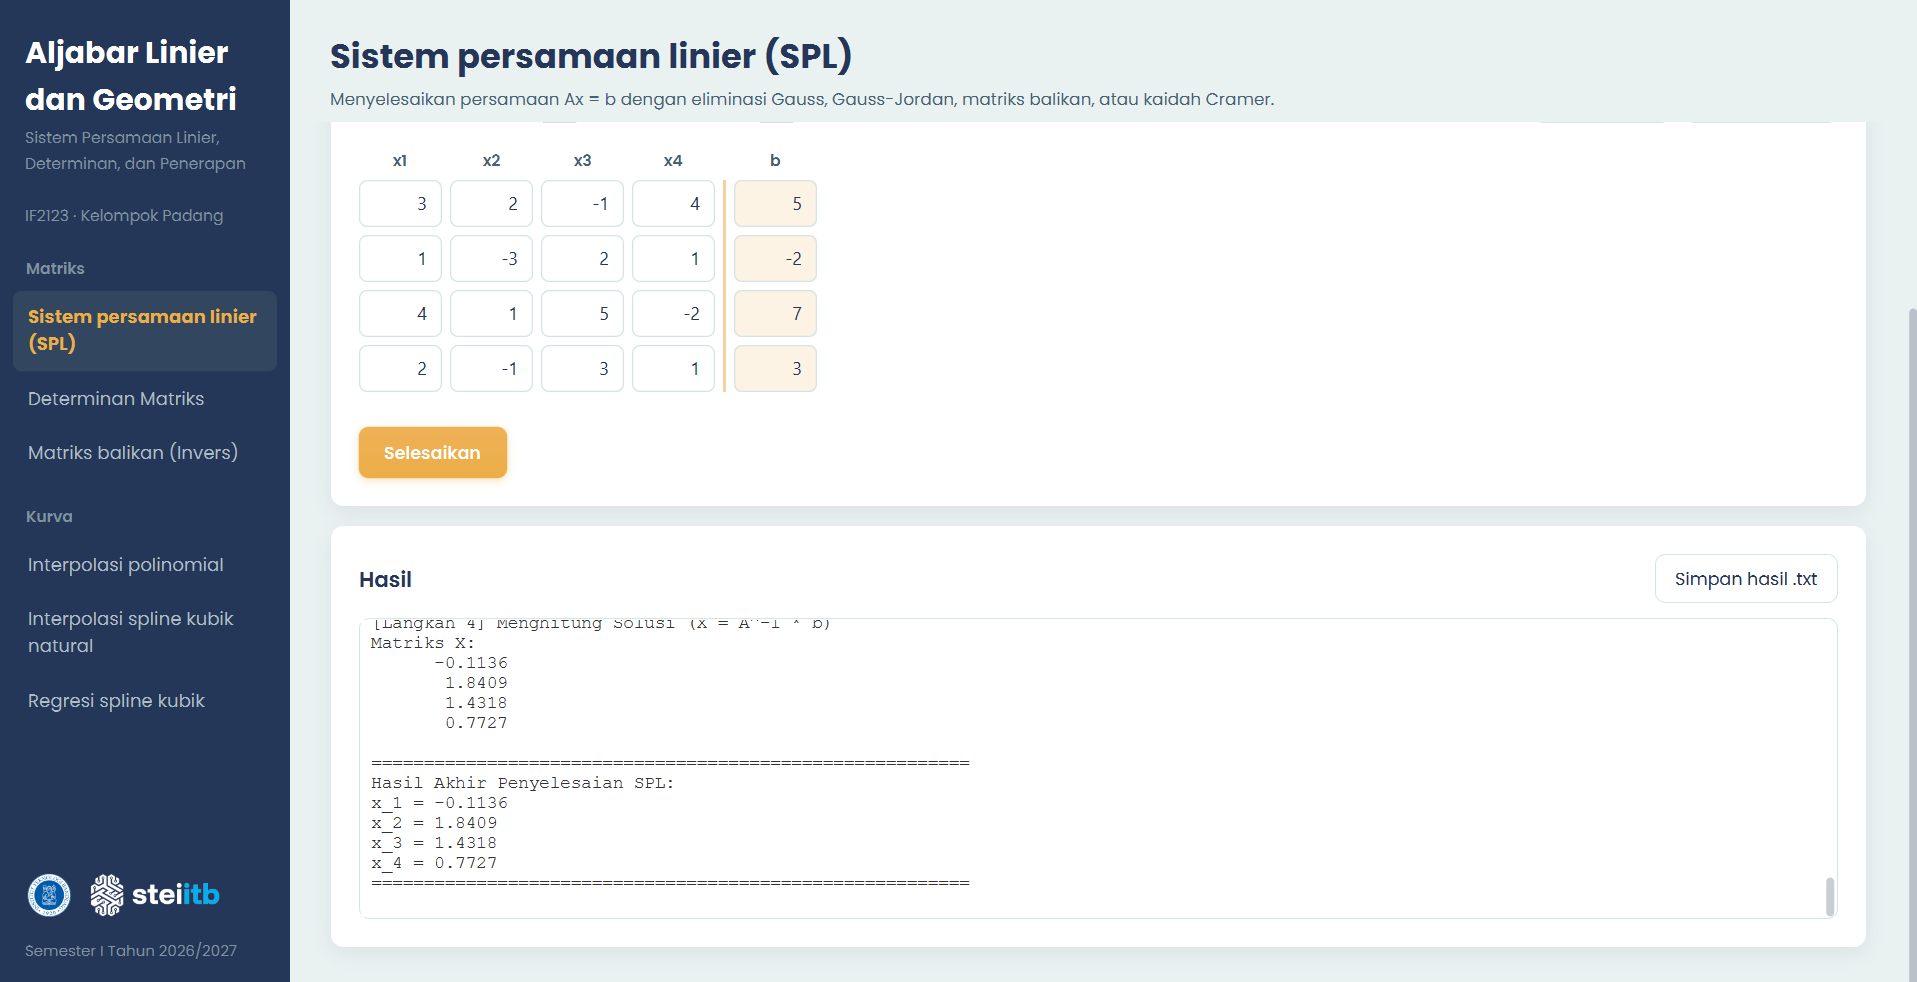
\includegraphics[width=0.8\textwidth]{5.5.1.invers.png}
    \caption{Penyelesaian SPL dengan Metode Invers}
\end{figure}
\begin{figure}[H]
    \centering
    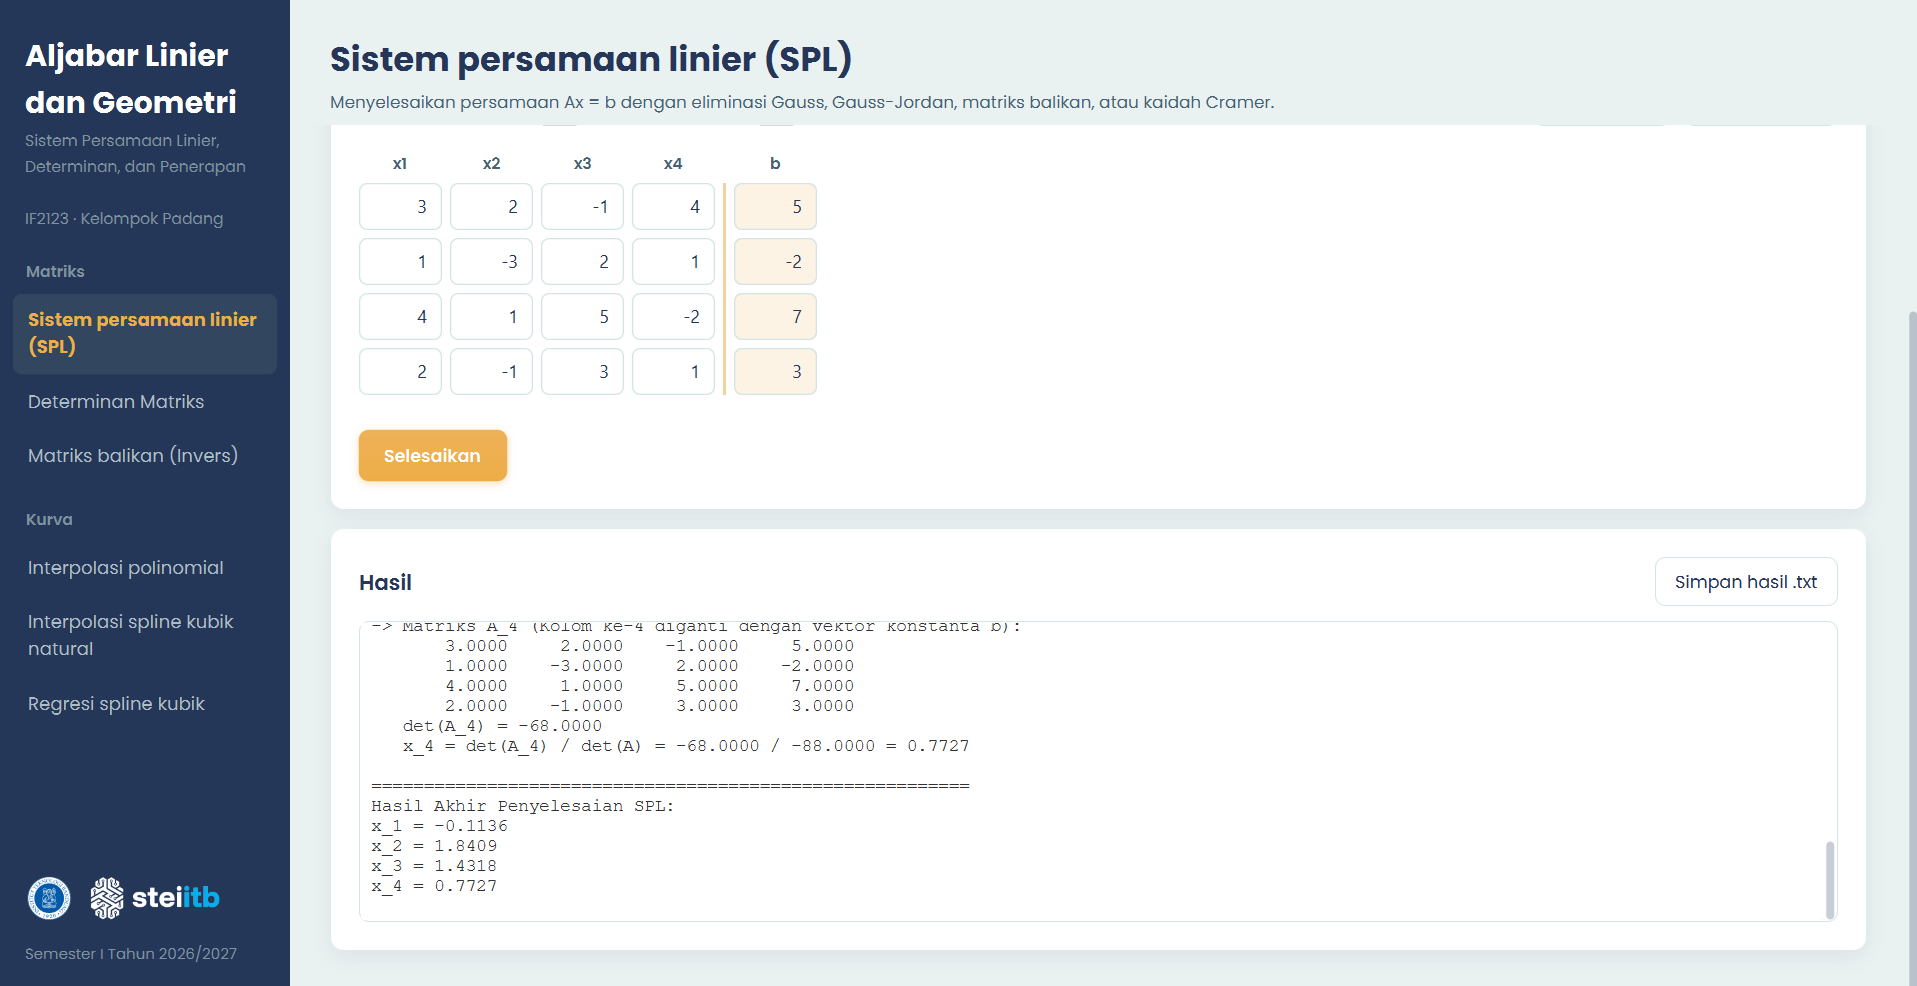
\includegraphics[width=0.8\textwidth]{5.5.1.cramer.png}
    \caption{Penyelesaian SPL dengan Kaidah Cramer}
\end{figure}

\textbf{Analisis:}
Seluruh metode, yaitu Eliminasi Gauss, Gauss-Jordan, Kaidah Cramer, dan Matriks Balikan, menghasilkan solusi tunggal yang konsisten. Karena determinan SPL tidak bernilai nol, SPL memiliki invers sehingga Kaidah Cramer dan Metode Matriks Balikan dapat diterapkan secara valid.

\subsection{Kasus Uji 4.5.2: SPL $9 \times 9$ }
\textbf{Sistem Persamaan Masukan (Bentuk Asli):}
\begin{align*}
x_1 + x_2 + x_3 &= 10.00 \\
x_4 + x_5 + x_6 &= 12.00 \\
x_7 + x_8 + x_9 &= 9.00 \\
0.03521(x_1 + x_4 + x_7) + 0.68(x_2 + x_6) + 0.55432x_9 &= 8.42 \\
0.87654(x_1 + x_4 + x_7) + 0.30(x_3 + x_5 + x_8) &= 11.05 \\
0.03521(x_1 + x_4 + x_7) + 0.68(x_3 + x_5) + 0.55432x_2 &= 6.19 \\
x_1 + x_5 + x_9 &= 11.00 \\
x_2 + x_4 + x_8 &= 8.50 \\
x_3 + x_6 + x_7 &= 11.50
\end{align*}

\textbf{Penjabaran Persamaan:}
\begin{align*}
1x_1 + 1x_2 + 1x_3 + 0x_4 + 0x_5 + 0x_6 + 0x_7 + 0x_8 + 0x_9 &= 10.00 \\
0x_1 + 0x_2 + 0x_3 + 1x_4 + 1x_5 + 1x_6 + 0x_7 + 0x_8 + 0x_9 &= 12.00 \\
0x_1 + 0x_2 + 0x_3 + 0x_4 + 0x_5 + 0x_6 + 1x_7 + 1x_8 + 1x_9 &= 9.00 \\
0.03521x_1 + 0.68x_2 + 0x_3 + 0.03521x_4 + 0x_5 + 0.68x_6 + 0.03521x_7 + 0x_8 + 0.55432x_9 &= 8.42 \\
0.87654x_1 + 0x_2 + 0.30x_3 + 0.87654x_4 + 0.30x_5 + 0x_6 + 0.87654x_7 + 0.30x_8 + 0x_9 &= 11.05 \\
0.03521x_1 + 0.55432x_2 + 0.68x_3 + 0.03521x_4 + 0.68x_5 + 0x_6 + 0.03521x_7 + 0x_8 + 0x_9 &= 6.19 \\
1x_1 + 0x_2 + 0x_3 + 0x_4 + 1x_5 + 0x_6 + 0x_7 + 0x_8 + 1x_9 &= 11.00 \\
0x_1 + 1x_2 + 0x_3 + 1x_4 + 0x_5 + 0x_6 + 0x_7 + 1x_8 + 0x_9 &= 8.50 \\
0x_1 + 0x_2 + 1x_3 + 0x_4 + 0x_5 + 1x_6 + 1x_7 + 0x_8 + 0x_9 &= 11.50
\end{align*}

\textbf{Hasil Eksekusi Program:}
\begin{figure}[H]
    \centering
    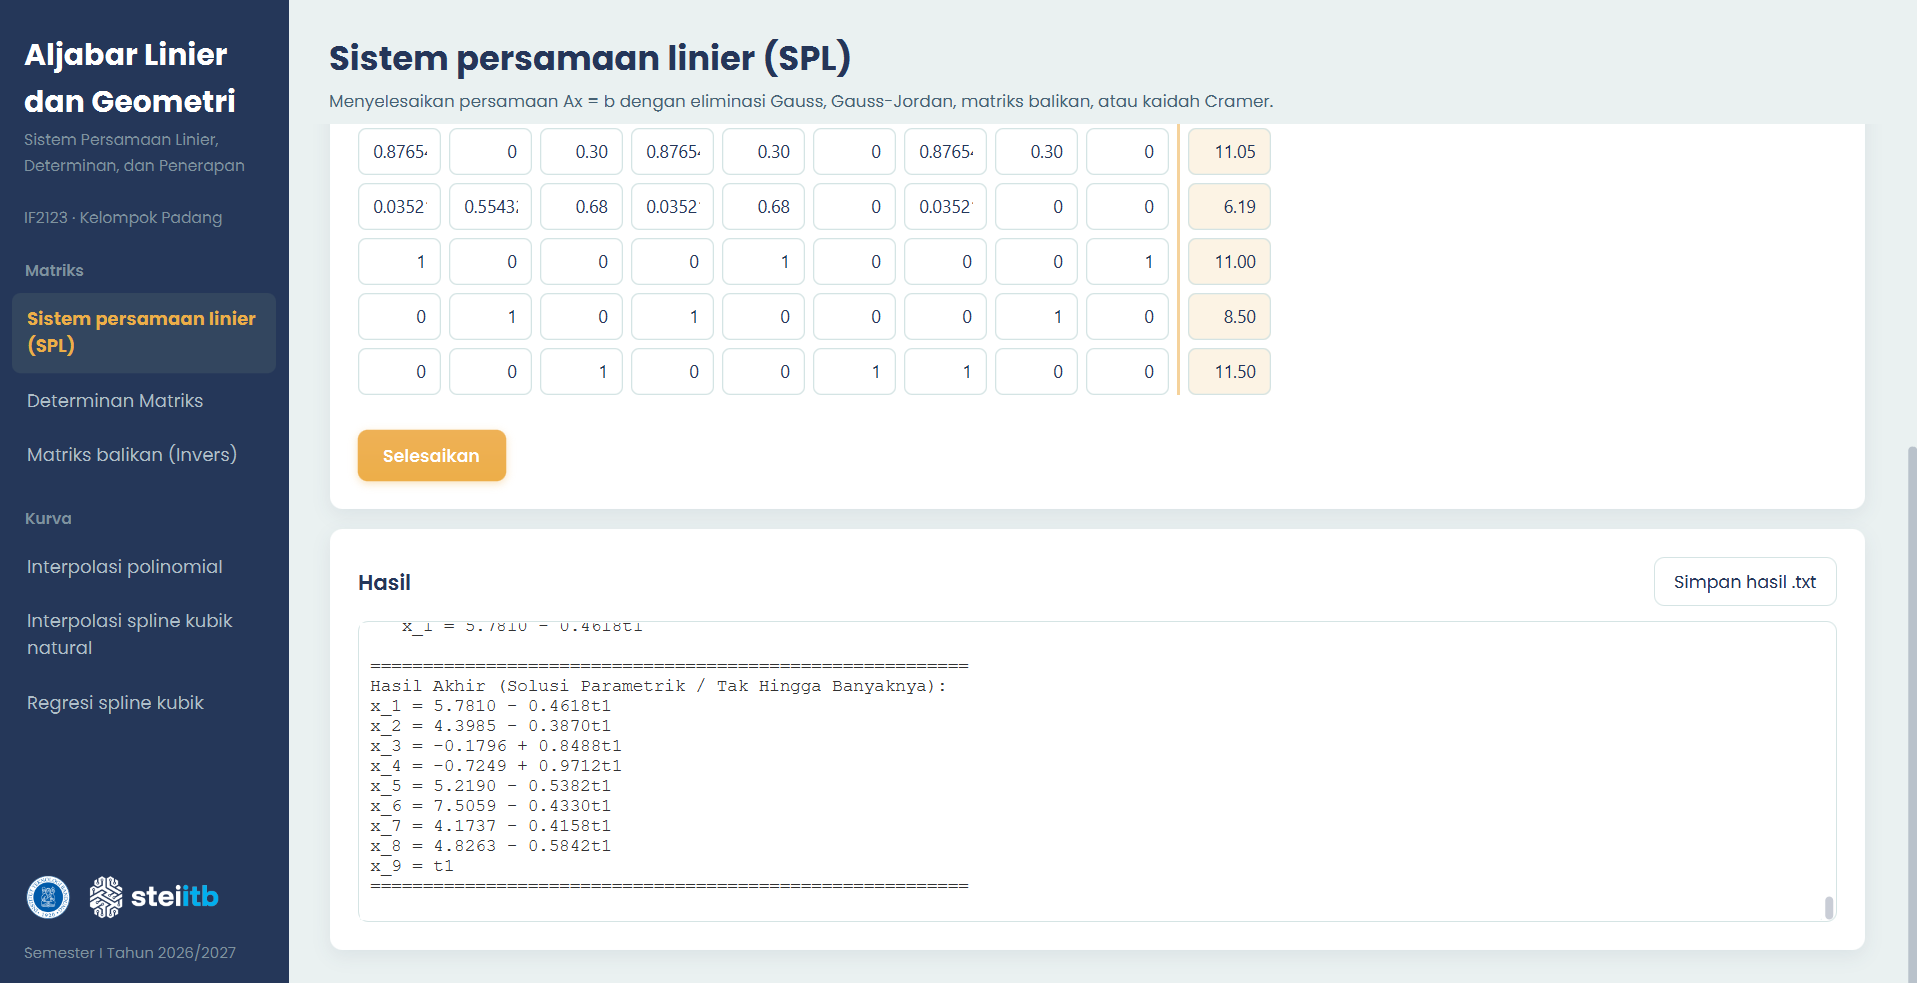
\includegraphics[width=0.8\textwidth]{5.5.2.gauss.png}
    \caption{Penyelesaian SPL dengan Metode Gauss}
\end{figure}
\begin{figure}[H]
    \centering
    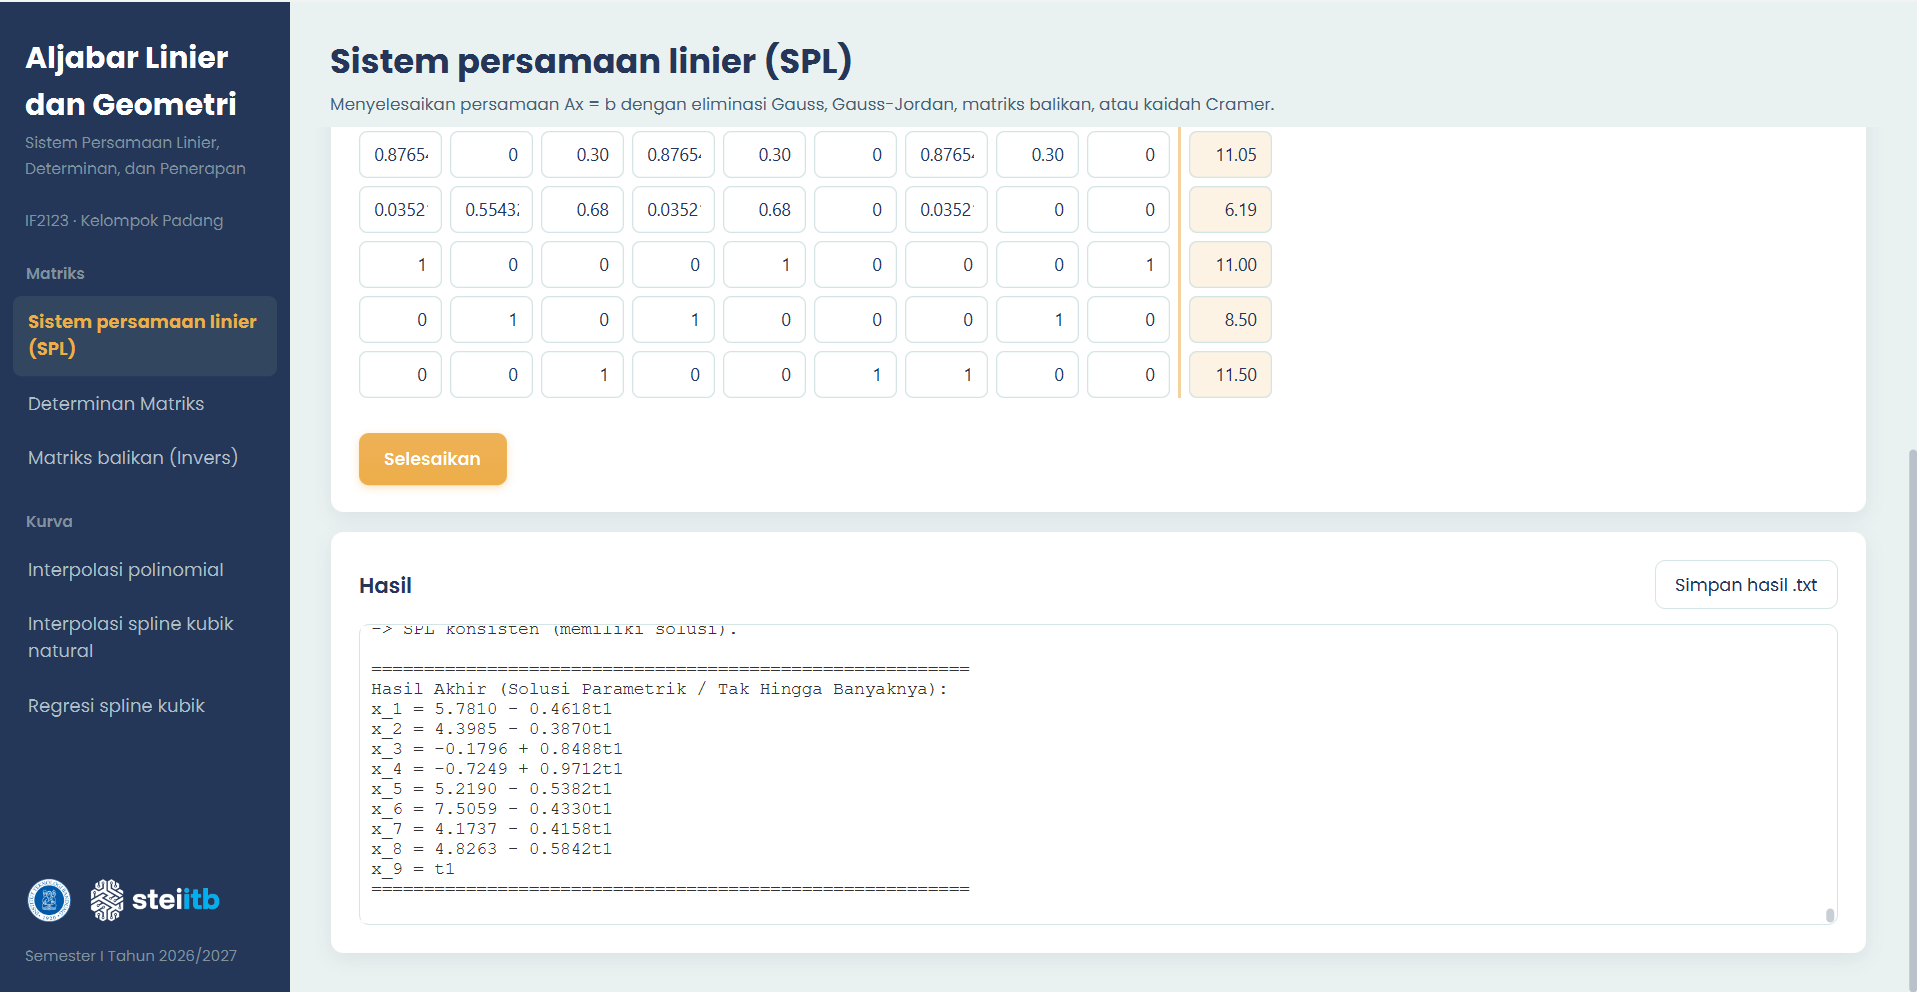
\includegraphics[width=0.8\textwidth]{5.5.2.gaussjordan.png}
    \caption{Penyelesaian SPL dengan Metode Gauss-Jordan}
\end{figure}
\begin{figure}[H]
    \centering
    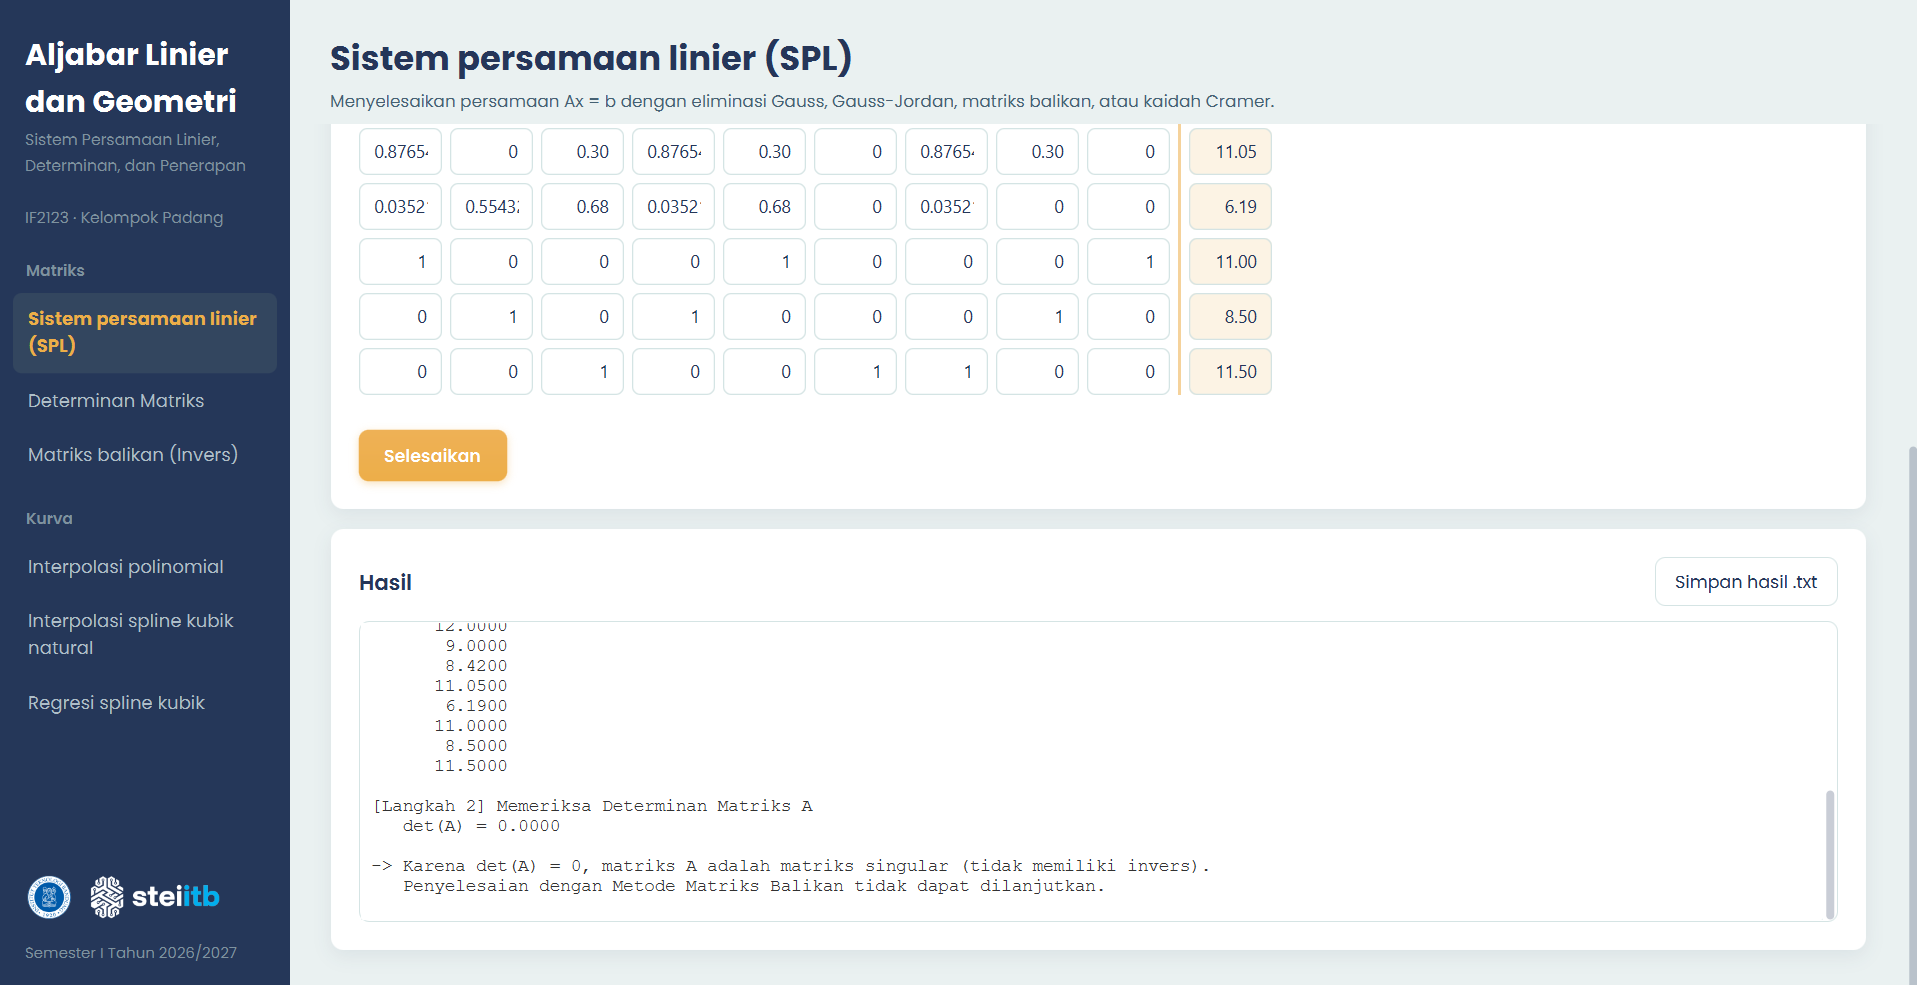
\includegraphics[width=0.8\textwidth]{5.5.2.invers.png}
    \caption{Penyelesaian SPL dengan Metode Invers}
\end{figure}
\begin{figure}[H]
    \centering
    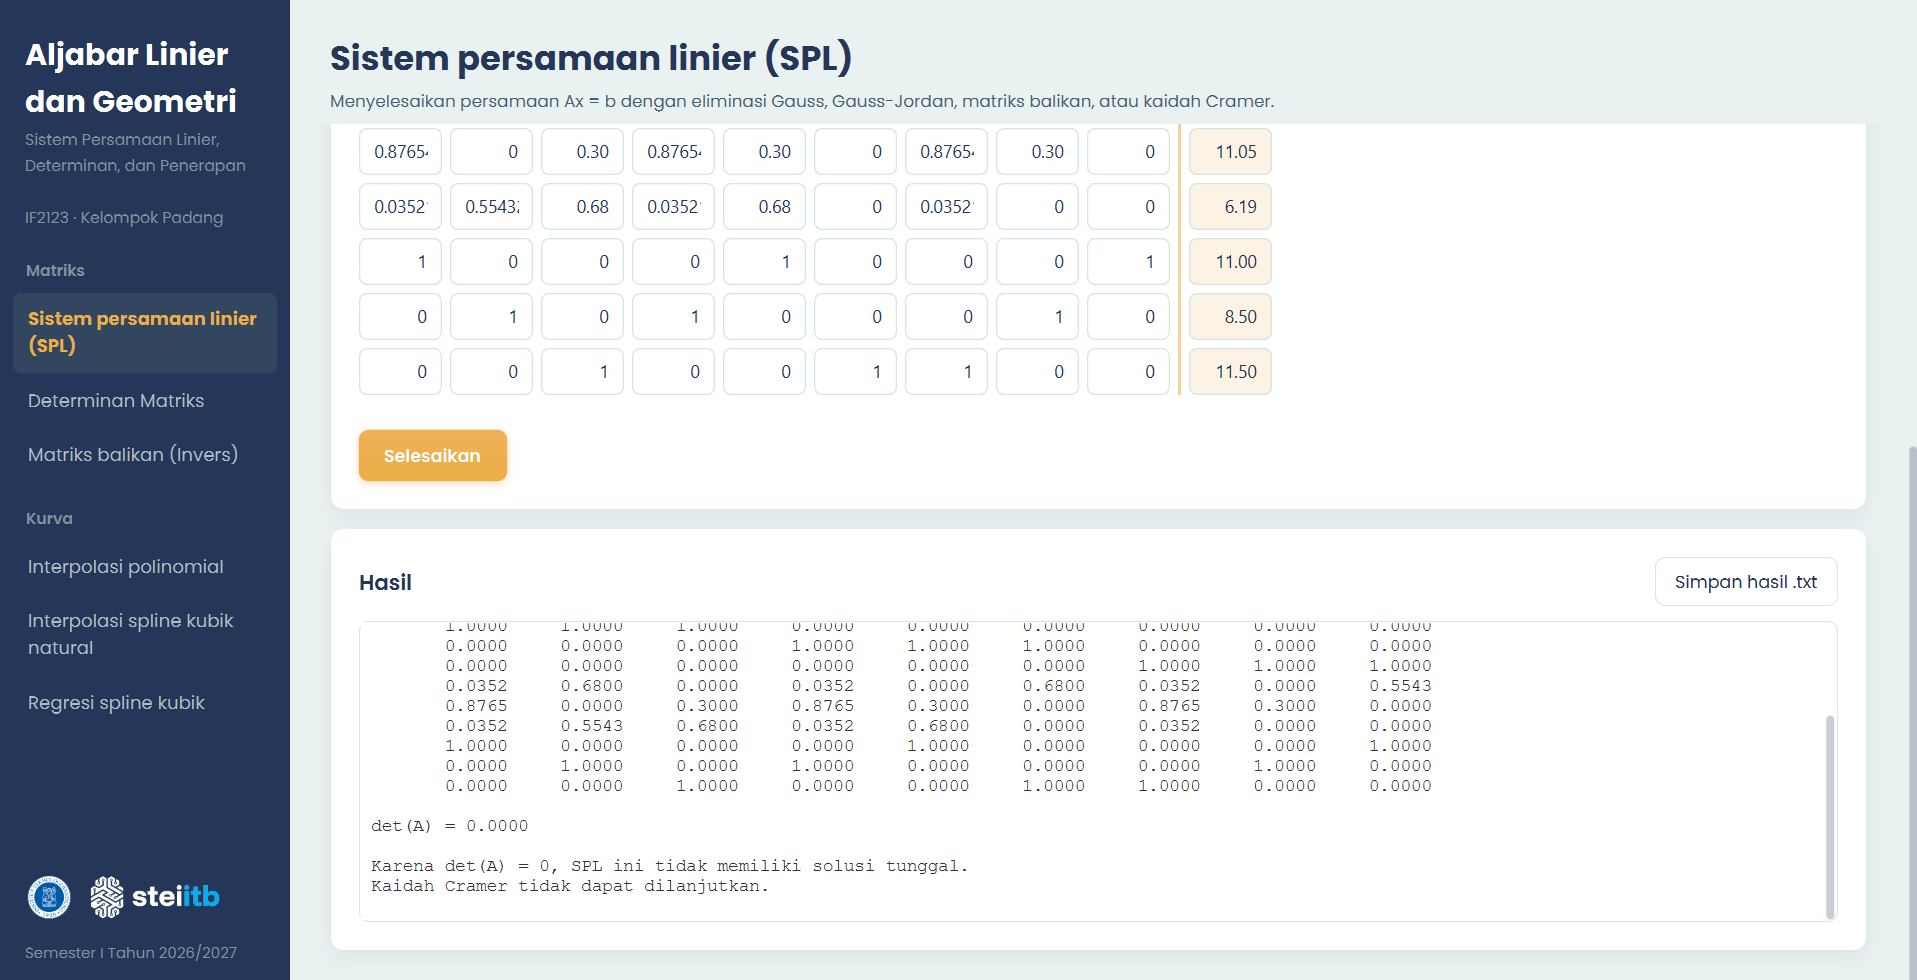
\includegraphics[width=0.8\textwidth]{5.5.2.cramer.png}
    \caption{Penyelesaian SPL dengan Kaidah Cramer}
\end{figure}

\textbf{Analisis:}
Berdasarkan hasil perhitungan dari metode Eliminasi Gauss dan Gauss-Jordan, SPL \(A\) memiliki solusi parametrik/tak hingga, tetapiSPL memiliki \(determinan = 0\) sehingga metode Kaidah Cramer dan Metode Matriks Balikan tidak dapat digunakan.

% 5.6 Aplikasi Sistem Persamaan Linier
\section{Kasus Uji 4.6: Aplikasi Sistem Persamaan Linier}

\textbf{Persamaan Masukan (Hasil Penjabaran):}
Substitusikan nilai dari dataset ke dalam persamaan:
\begin{align*}
3\theta_0 + (1 + 2 + 3)\theta_1 &= 3 + 5 + 6 \\
(1 + 2 + 3)\theta_0 + (1^2 + 2^2 + 3^2)\theta_1 &= (1)(3) + (2)(5) + (3)(6)
\end{align*}

Sehingga sistem persamaan linear yang siap dimasukkan ke kalkulator (dengan memisalkan \(x_1 = \theta_0\) dan \(x_2 = \theta_1\)) adalah:
\begin{align*}
3x_1 + 6x_2 &= 14 \\
6x_1 + 14x_2 &= 31
\end{align*}

\textbf{Hasil Eksekusi Program:}
\begin{figure}[H]
    \centering
    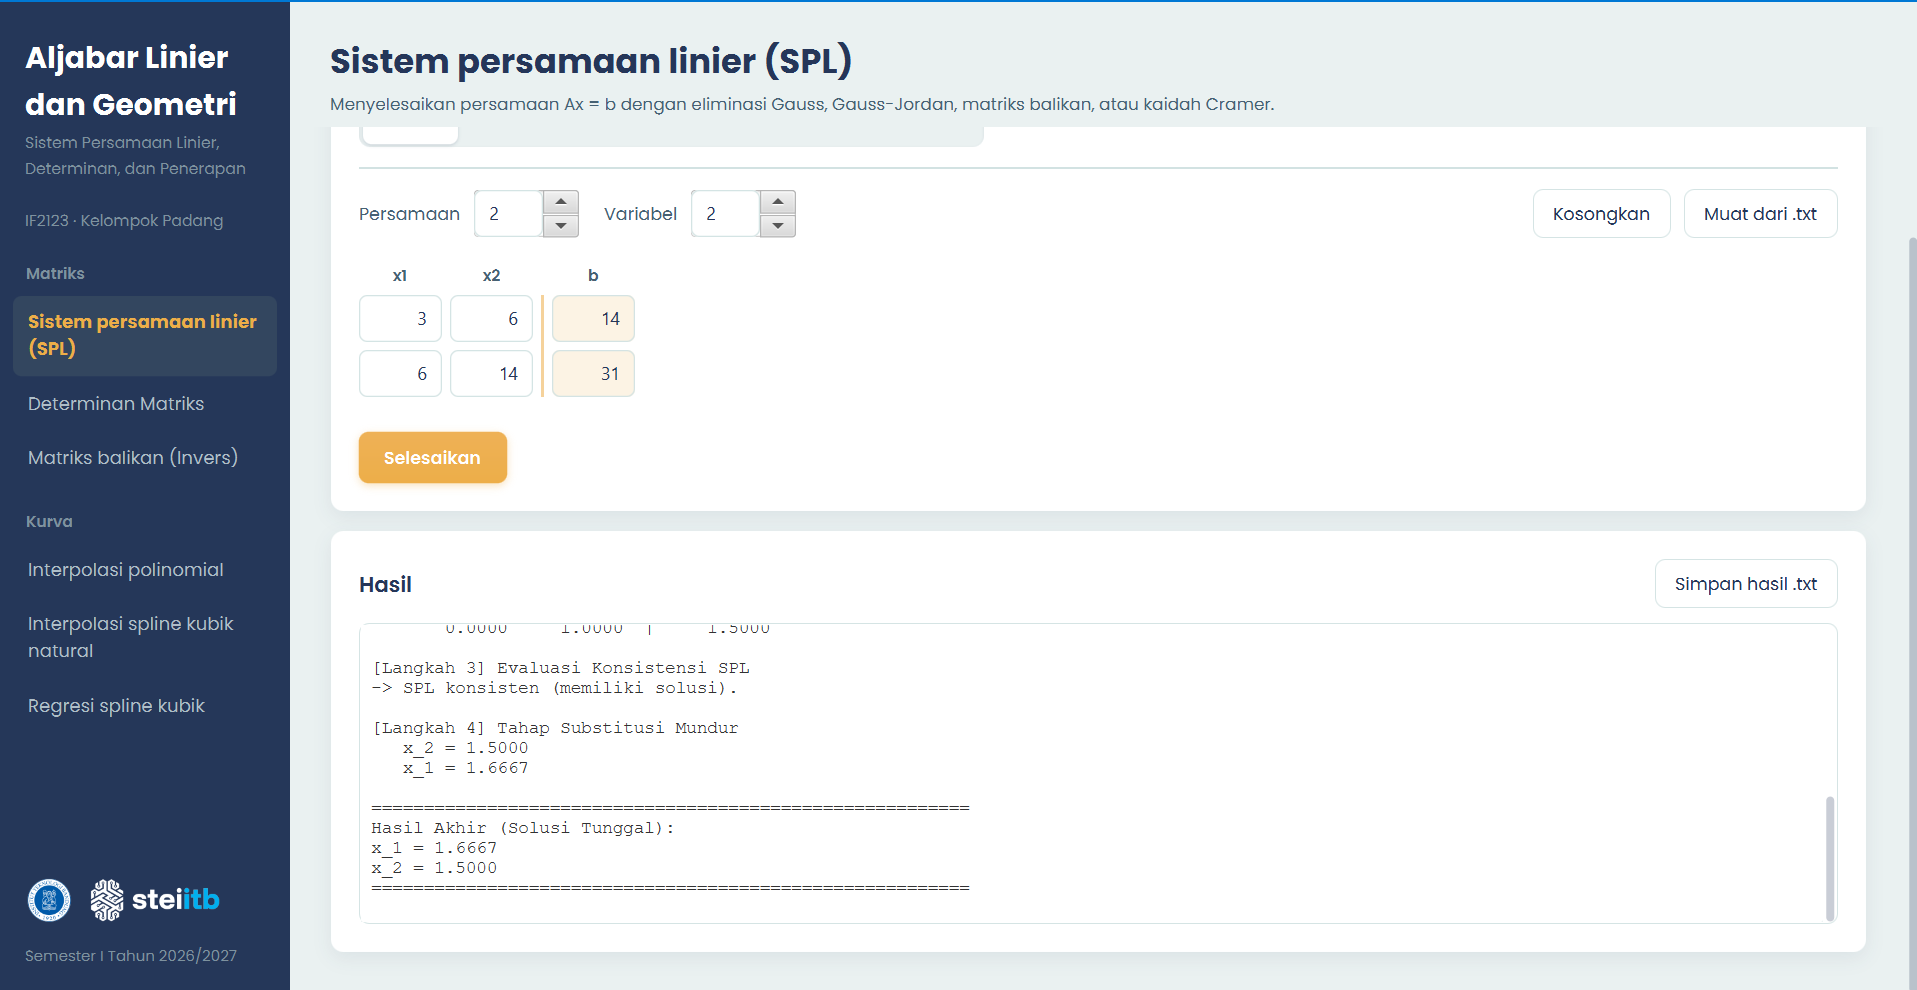
\includegraphics[width=0.8\textwidth]{5.6.gauss.png}
    \caption{Hasil Metode Gauss Kasus Uji 5.6}
\end{figure}
\begin{figure}[H]
    \centering
    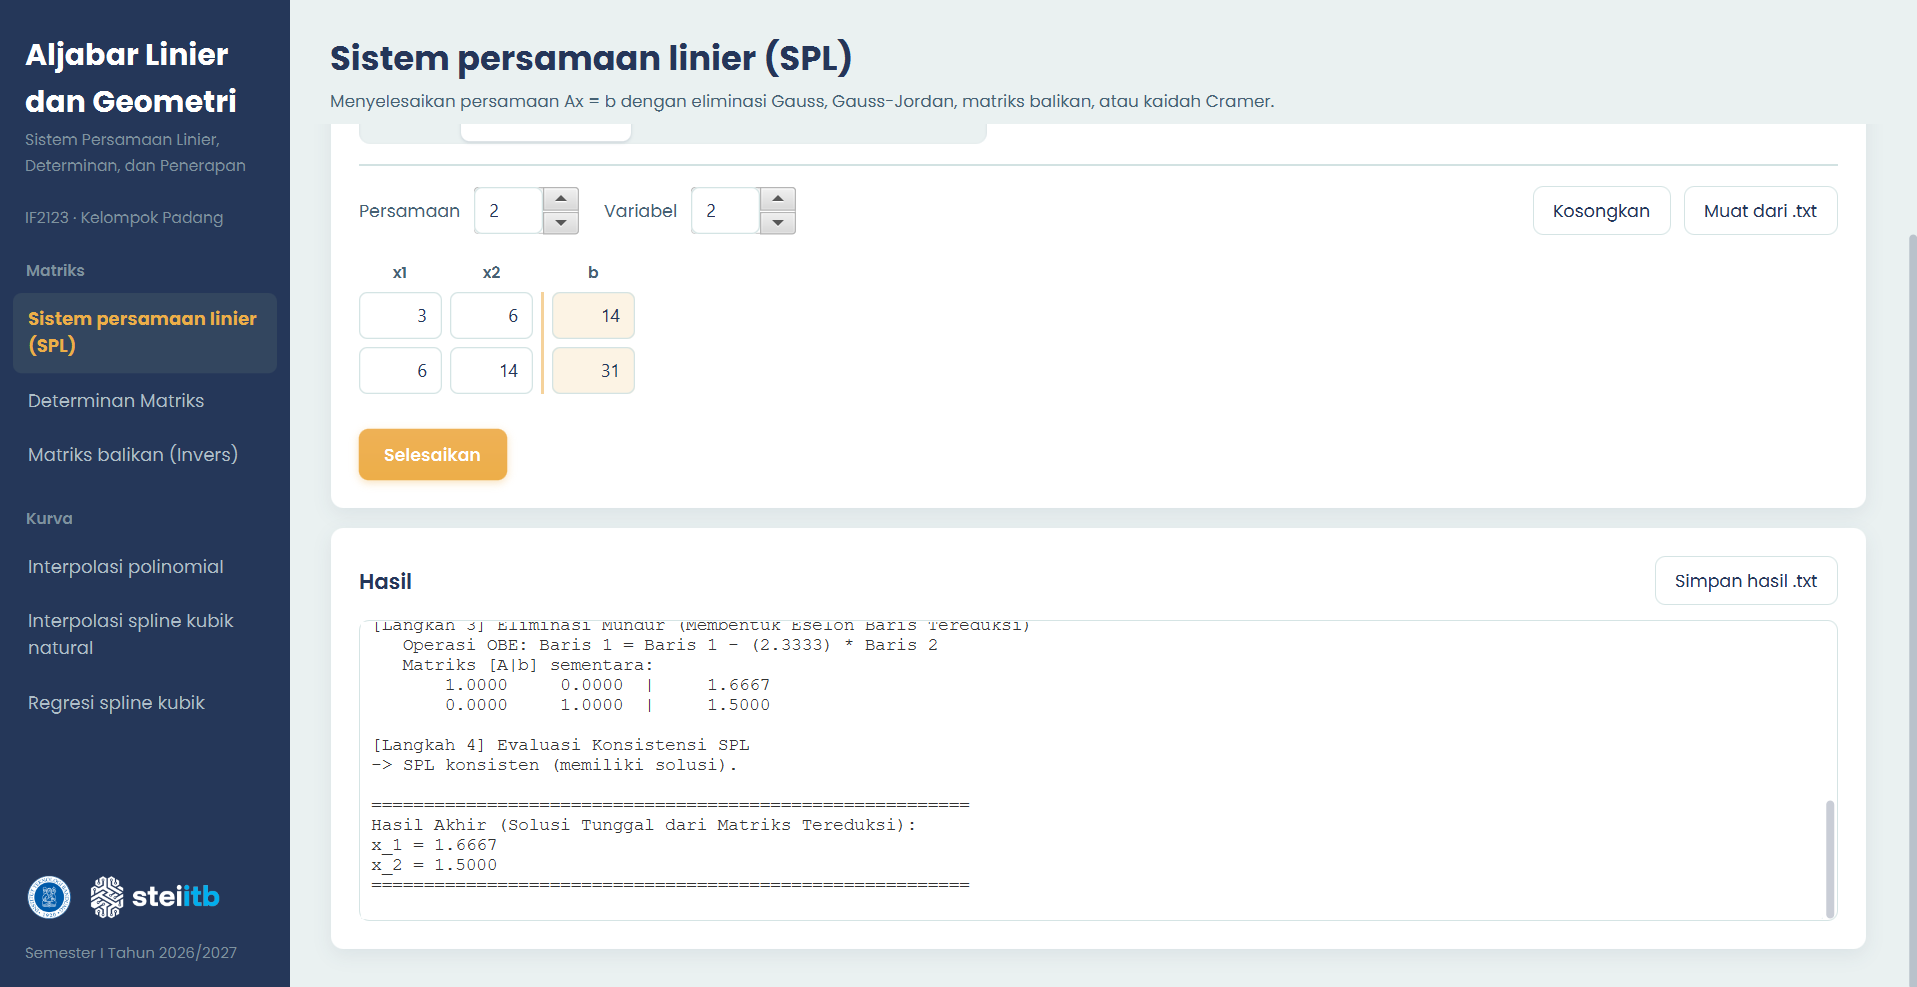
\includegraphics[width=0.8\textwidth]{5.6.gaussjordan.png}
    \caption{Hasil Metode Gauss-Jordan Kasus Uji 5.6}
\end{figure}
\begin{figure}[H]
    \centering
    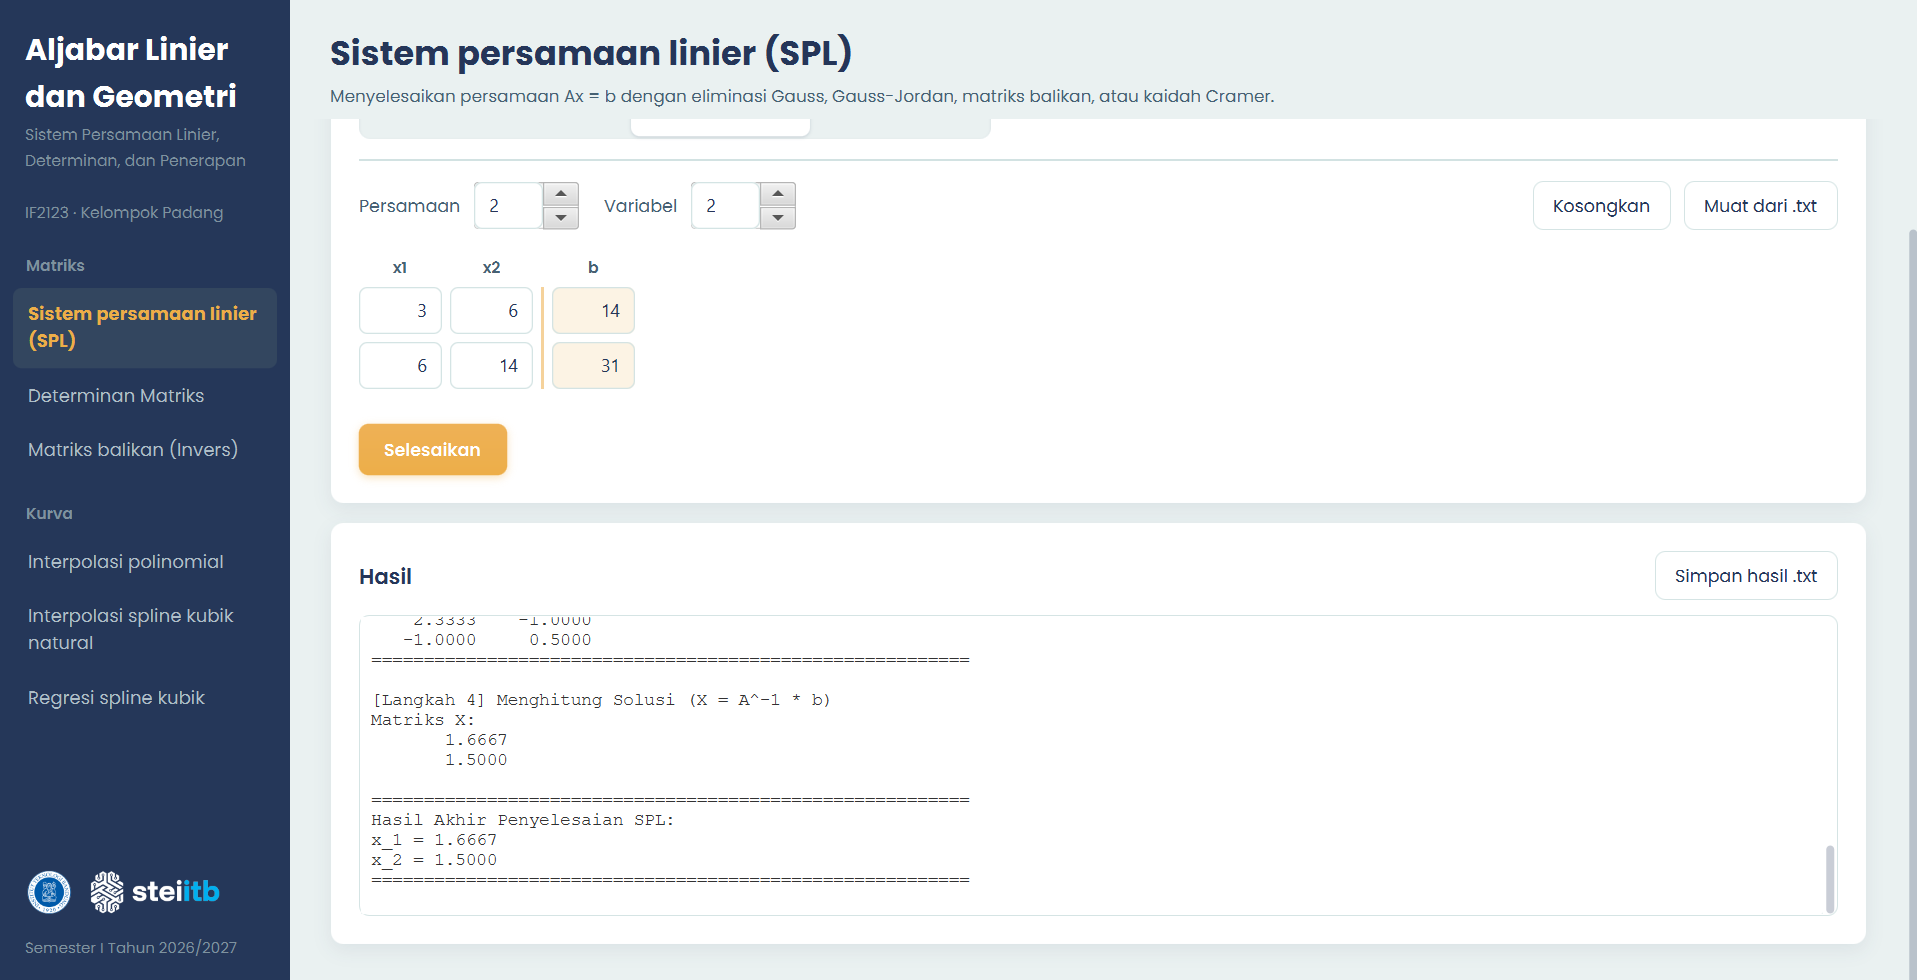
\includegraphics[width=0.8\textwidth]{5.6.invers.png}
    \caption{Hasil Metode Invers Kasus Uji 5.6}
\end{figure}
\begin{figure}[H]
    \centering
    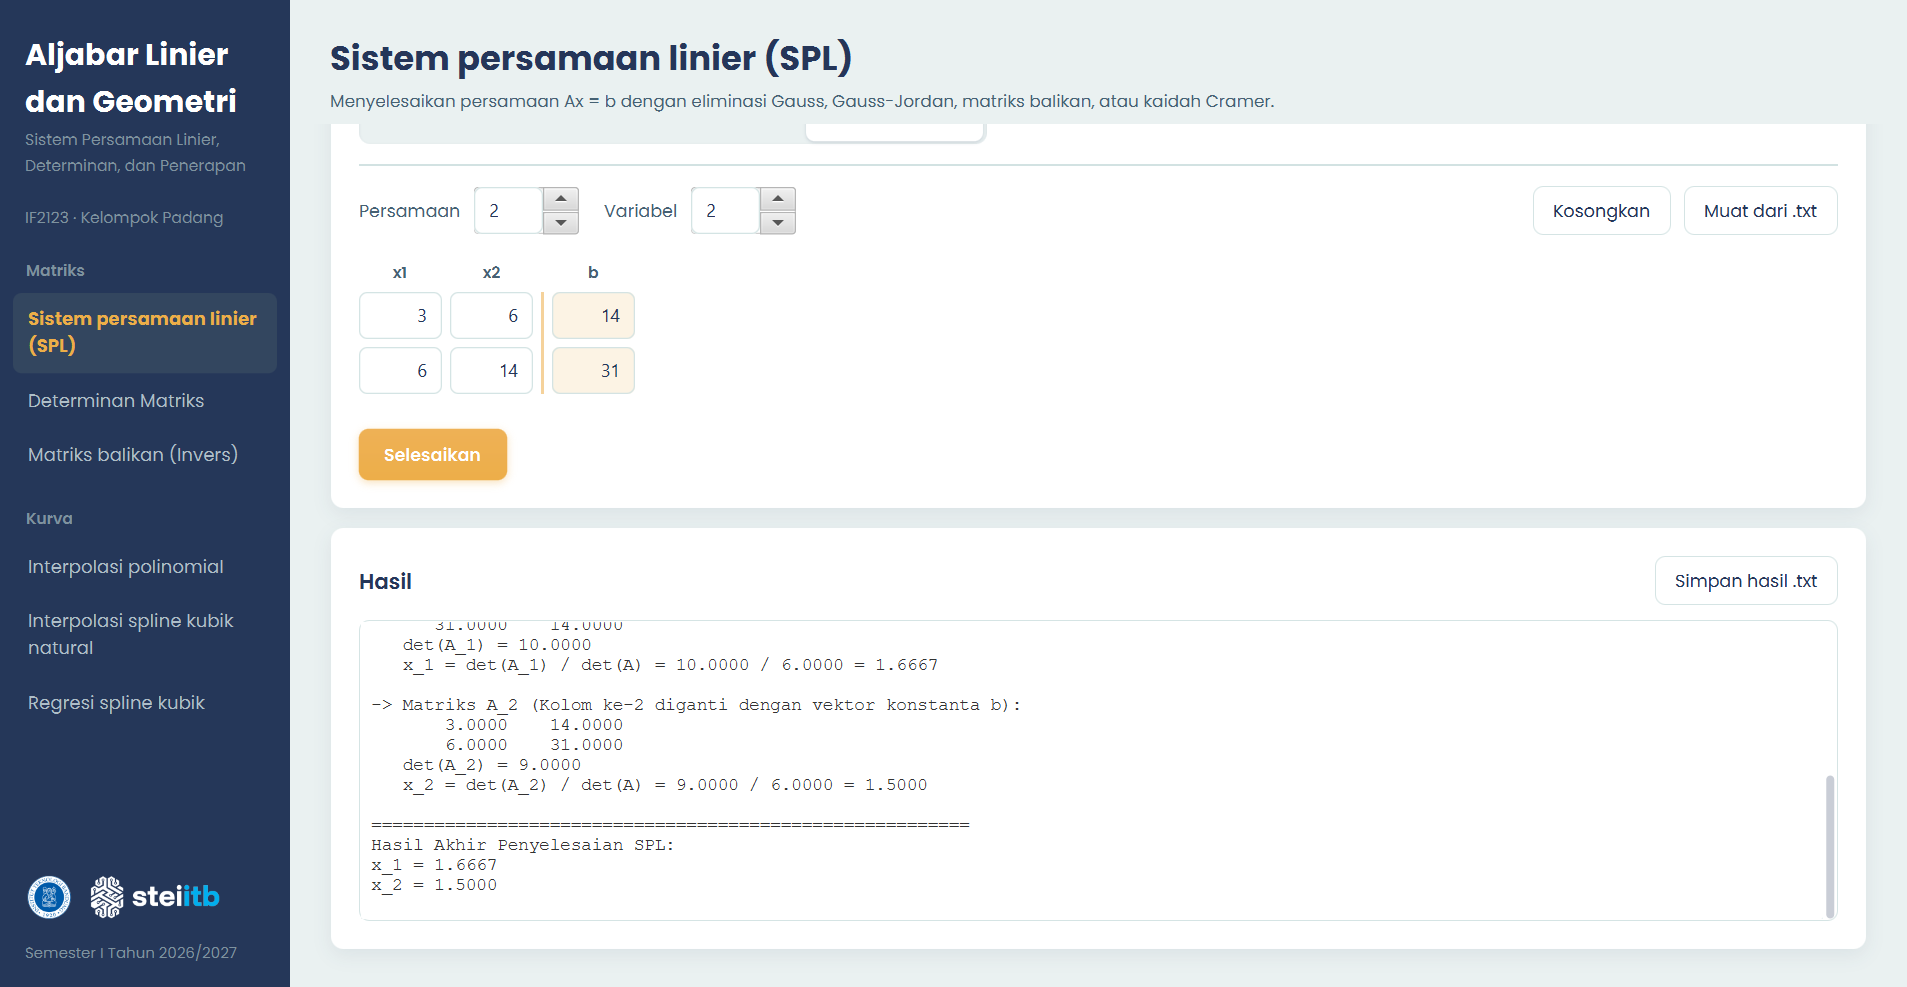
\includegraphics[width=0.8\textwidth]{5.6.cramer.png}
    \caption{Hasil Metode Cramer Kasus Uji 5.6}
\end{figure}

\textbf{Analisis:}
Seluruh metode, yaitu Eliminasi Gauss, Gauss-Jordan, Kaidah Cramer, dan Matriks Balikan, menghasilkan solusi tunggal yang konsisten. Karena determinan SPL tidak bernilai nol, SPL memiliki invers sehingga Kaidah Cramer dan Metode Matriks Balikan dapat diterapkan secara valid.

% 5.7 Interpolasi Polinomial
\section{Kasus Uji 4.7: Interpolasi Polinomial}

\subsection{Kasus Uji 4.7.1: Tujuh Titik Data (Domain $[0{,}2;\, 1{,}4]$)}
\textbf{Titik Data Masukan:}

\begin{table}[H]
    \centering
    \begin{tabular}{|c|c|c|c|c|c|c|c|}
        \hline
        \textbf{$x$} & 0,2 & 0,4 & 0,6 & 0,8 & 1,0 & 1,2 & 1,4 \\
        \hline
        \textbf{$y$} & 0,182 & 0,336 & 0,47 & 0,588 & 0,693 & 0,788 & 0,875 \\
        \hline
    \end{tabular}
    \caption{Titik Data Masukan Kasus Uji 4.7.1}
\end{table}

\textbf{Hasil Eksekusi Program:}
\begin{figure}[H]
    \centering
    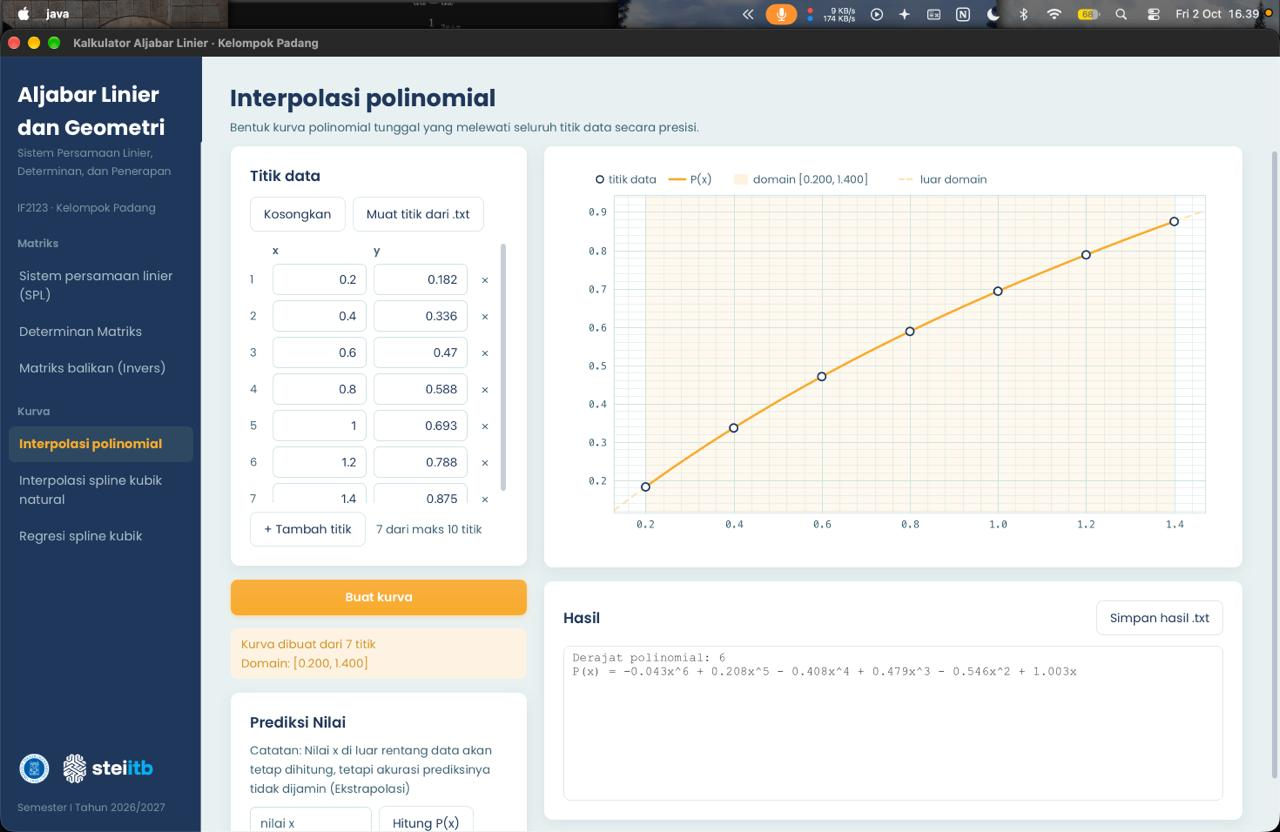
\includegraphics[width=0.8\textwidth]{interpolasi_polinomial1.jpeg}
    \caption{Hasil Interpolasi Polinomial Kasus Uji 5.7.1}
\end{figure}

\textbf{Analisis:}
Program menerima tujuh titik data sehingga polinomial interpolasi yang dihasilkan berderajat enam, yaitu
\[
P(x) = -0{,}043x^6 + 0{,}208x^5 - 0{,}408x^4 + 0{,}479x^3 - 0{,}546x^2 + 1{,}003x.
\]
Kurva $P(x)$ melewati seluruh titik data pada domain $[0{,}2;\, 1{,}4]$ dan berbentuk menaik secara mulus dengan kelengkungan yang makin landai, menyerupai pola fungsi logaritmik. Bagian kurva di luar domain digambar putus-putus karena nilainya merupakan hasil ekstrapolasi, sehingga akurasinya tidak dijamin.

\subsection{Kasus Uji 4.7.2: Enam Titik Data (Domain $[0;\, 10]$)}
\textbf{Titik Data Masukan:}

\begin{table}[H]
    \centering
    \begin{tabular}{|c|c|c|c|c|c|c|}
        \hline
        \textbf{$x$} & 0 & 2 & 4 & 6 & 8 & 10 \\
        \hline
        \textbf{$y$} & 25 & 31,2 & 38,6 & 47,5 & 58,1 & 70,8 \\
        \hline
    \end{tabular}
    \caption{Titik Data Masukan Kasus Uji 4.7.2}
\end{table}

\textbf{Hasil Eksekusi Program:}
\begin{figure}[H]
    \centering
    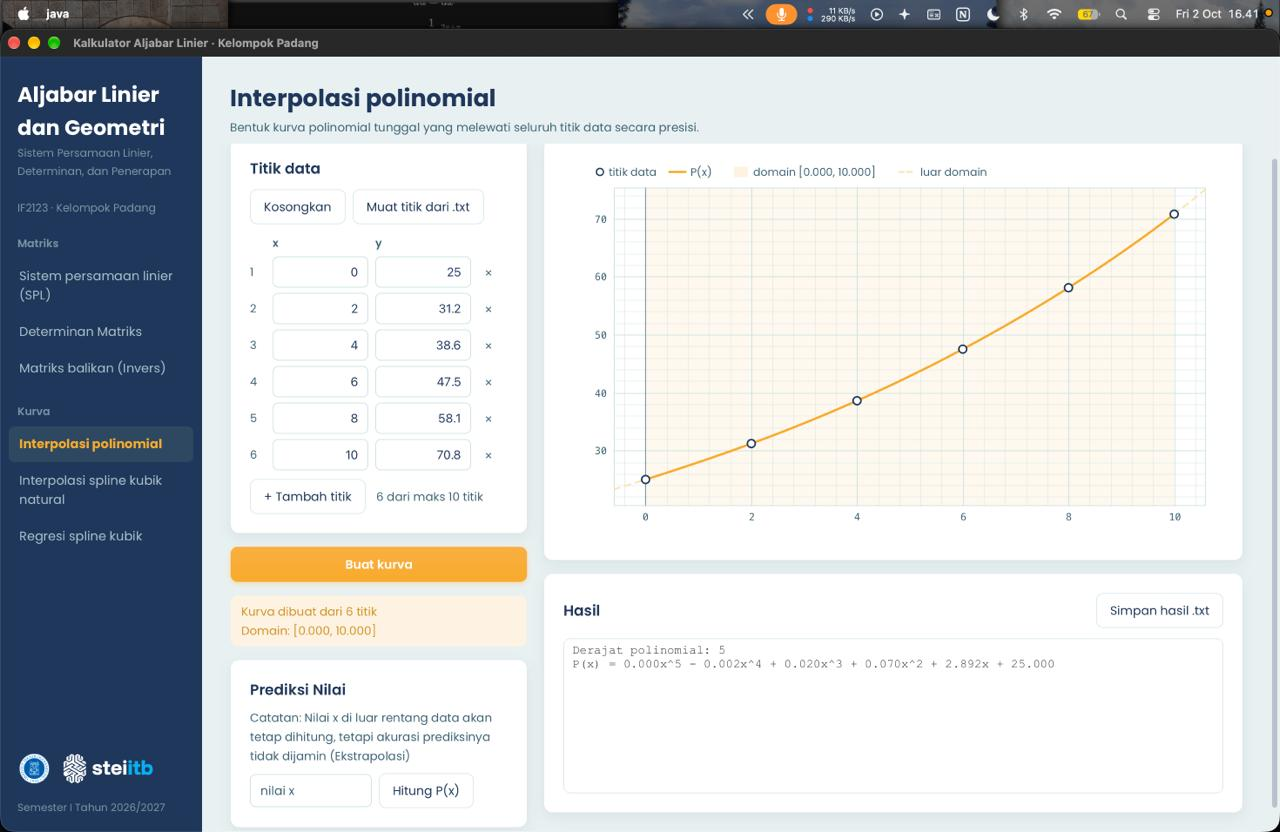
\includegraphics[width=0.8\textwidth]{interpolasi_polinomial2.jpeg}
    \caption{Hasil Interpolasi Polinomial Kasus Uji 4.7.2}
\end{figure}

\textbf{Analisis:}
Enam titik data menghasilkan polinomial berderajat lima, yaitu
\[
P(x) = 0{,}000x^5 - 0{,}002x^4 + 0{,}020x^3 + 0{,}070x^2 + 2{,}892x + 25{,}000.
\]
Suku $x^5$ bernilai sangat kecil sehingga tampil sebagai $0{,}000$ pada pembulatan tiga angka desimal, dan suku konstan $25{,}000$ sesuai dengan titik pertama $(0,\, 25)$. Kurva melewati seluruh titik data dan menunjukkan tren naik yang makin curam seiring bertambahnya $x$.

\subsection{Kasus Uji 4.7.3: Tiga Titik Data}
\textbf{Titik Data Masukan:}

\begin{table}[H]
    \centering
    \begin{tabular}{|c|c|c|c|}
        \hline
        \textbf{$x$} & 1 & 3 & 5 \\
        \hline
        \textbf{$y$} & 2 & 6 & 4 \\
        \hline
    \end{tabular}
    \caption{Titik Data Masukan Kasus Uji 4.7.3}
\end{table}

\textbf{Hasil Eksekusi Program:}
\begin{figure}[H]
    \centering
    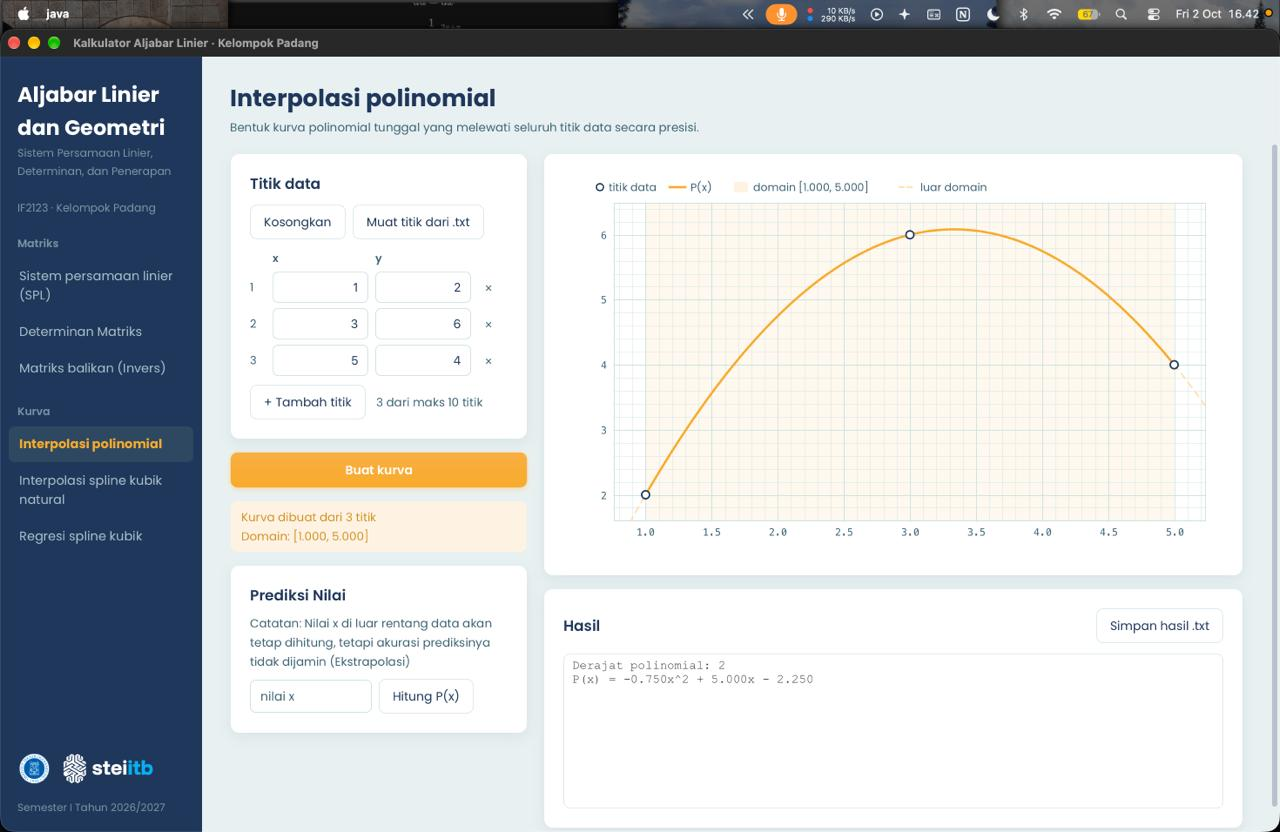
\includegraphics[width=0.8\textwidth]{interpolasi_polinomial3.jpeg}
    \caption{Hasil Interpolasi Polinomial Kasus Uji 4.7.3}
\end{figure}

\textbf{Analisis:}
Tiga titik data menghasilkan polinomial berderajat dua, yaitu
\[
P(x) = -0{,}750x^2 + 5{,}000x - 2{,}250.
\]
Substitusi $x = 1$, $x = 3$, dan $x = 5$ menghasilkan $P(x) = 2$, $6$, dan $4$, sehingga kurva tepat melewati ketiga titik. Koefisien $x^2$ yang negatif membuat parabola membuka ke bawah dengan titik puncak di sekitar $x \approx 3{,}33$ dan $P(x) \approx 6{,}083$, yang sesuai dengan bentuk kurva pada grafik.

% 5.8 Studi Interpolasi Natural Cubic Spline
\section{Kasus Uji 4.8: Studi Interpolasi Natural Cubic Spline}

\subsection{Kasus Uji 4.8.1: Lima Titik Data}
\textbf{Titik Data Masukan:}

\begin{table}[H]
    \centering
    \begin{tabular}{|c|c|c|c|c|c|}
        \hline
        \textbf{$x$} & 1 & 2 & 3 & 4 & 5 \\
        \hline
        \textbf{$y$} & 2 & 3 & 4 & 5 & 6 \\
        \hline
    \end{tabular}
    \caption{Titik Data Masukan Kasus Uji 4.8.1}
\end{table}

\textbf{Hasil Eksekusi Program:}
\begin{figure}[H]
    \centering
    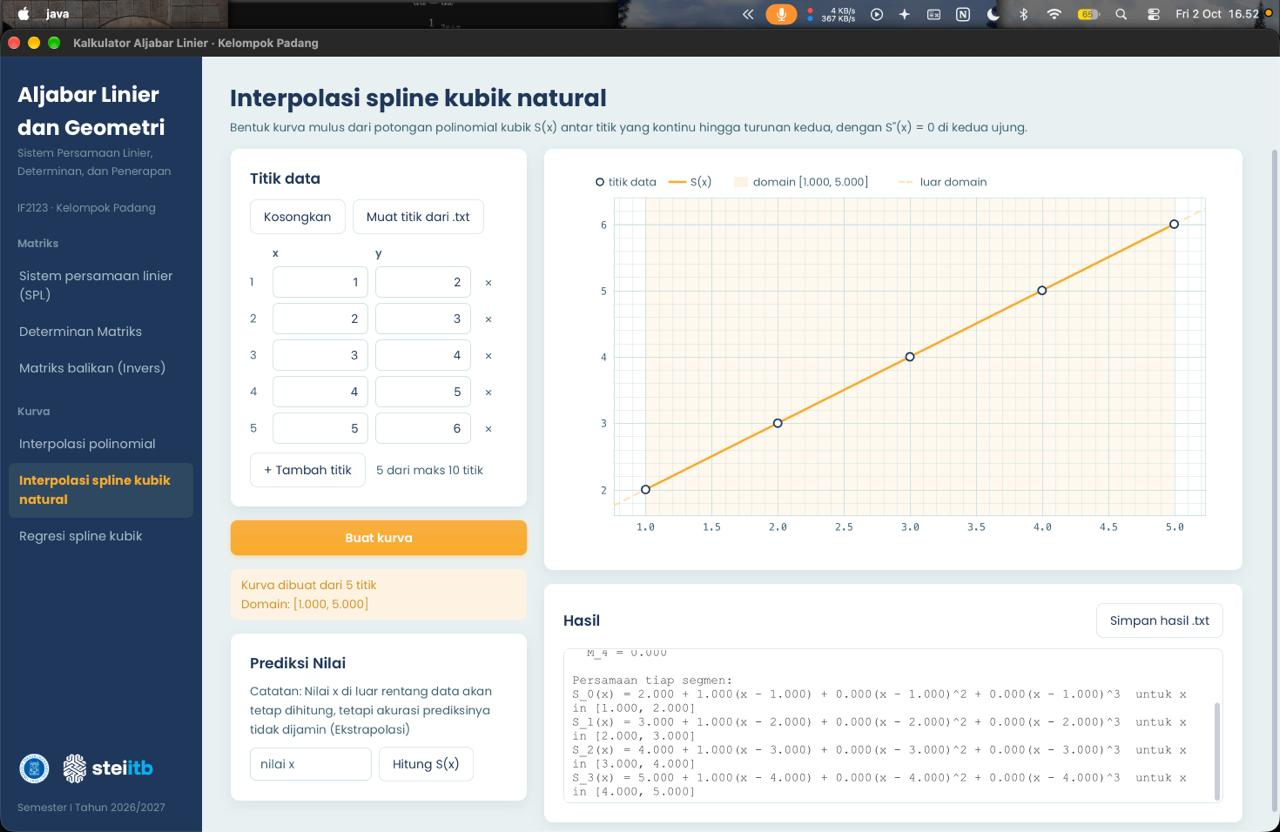
\includegraphics[width=0.8\textwidth]{interpolasi_spline_kubik.jpeg}
    \caption{Hasil Interpolasi Natural Cubic Spline Kasus Uji 4.8.1}
\end{figure}

\textbf{Analisis:}
Lima titik data membentuk empat segmen polinomial kubik $S_0(x)$ sampai $S_3(x)$ pada selang $[1,2]$, $[2,3]$, $[3,4]$, dan $[4,5]$. Setiap segmen berbentuk
\[
S_j(x) = a_j + b_j(x - x_j) + c_j(x - x_j)^2 + d_j(x - x_j)^3,
\]
dengan $b_j = 1{,}000$ serta $c_j = d_j = 0{,}000$ pada seluruh segmen, misalnya $S_0(x) = 2 + 1(x - 1)$. Titik-titik data ini terletak pada garis lurus $y = x + 1$, sehingga seluruh nilai momen kedua $M_i$ yang memenuhi syarat \textit{natural} ($M_0 = M_n = 0$) bernilai nol dan spline yang diperoleh berimpit dengan garis tersebut. Hasil ini sesuai dengan kurva pada grafik, yaitu garis lurus yang melewati seluruh titik data.

% 4.9 Studi Kasus Regresi Spline
\section{Kasus Uji 4.9: Studi Kasus Regresi Spline}

\subsection{Kasus Uji 4.9.1}
\textbf{Dataset Masukan:}
Dataset terdiri dari $N = 7$ titik data berjarak seragam pada domain $[-3, 3]$ dengan pola non-linear (menurun lalu naik tajam). Regresi spline kubik dilakukan dengan satu knot di posisi $\xi = 0$ ($K = 1$), sehingga jumlah basis $M = K + 4 = 5$.

\begin{table}[H]
    \centering
    \begin{tabular}{|c|c|c|}
        \hline
        \textbf{$i$} & \textbf{$x$} & \textbf{$y$} \\
        \hline
        1 & $-3$ & $19{,}9$ \\
        2 & $-2$ & $4{,}4$ \\
        3 & $-1$ & $-0{,}5$ \\
        4 & $0$  & $2{,}0$ \\
        5 & $1$  & $6{,}5$ \\
        6 & $2$  & $15{,}6$ \\
        7 & $3$  & $38{,}1$ \\
        \hline
    \end{tabular}
    \caption{Dataset Masukan Studi Kasus Regresi Spline}
\end{table}

\textbf{Hasil Eksekusi Program:}
\begin{figure}[H]
    \centering
    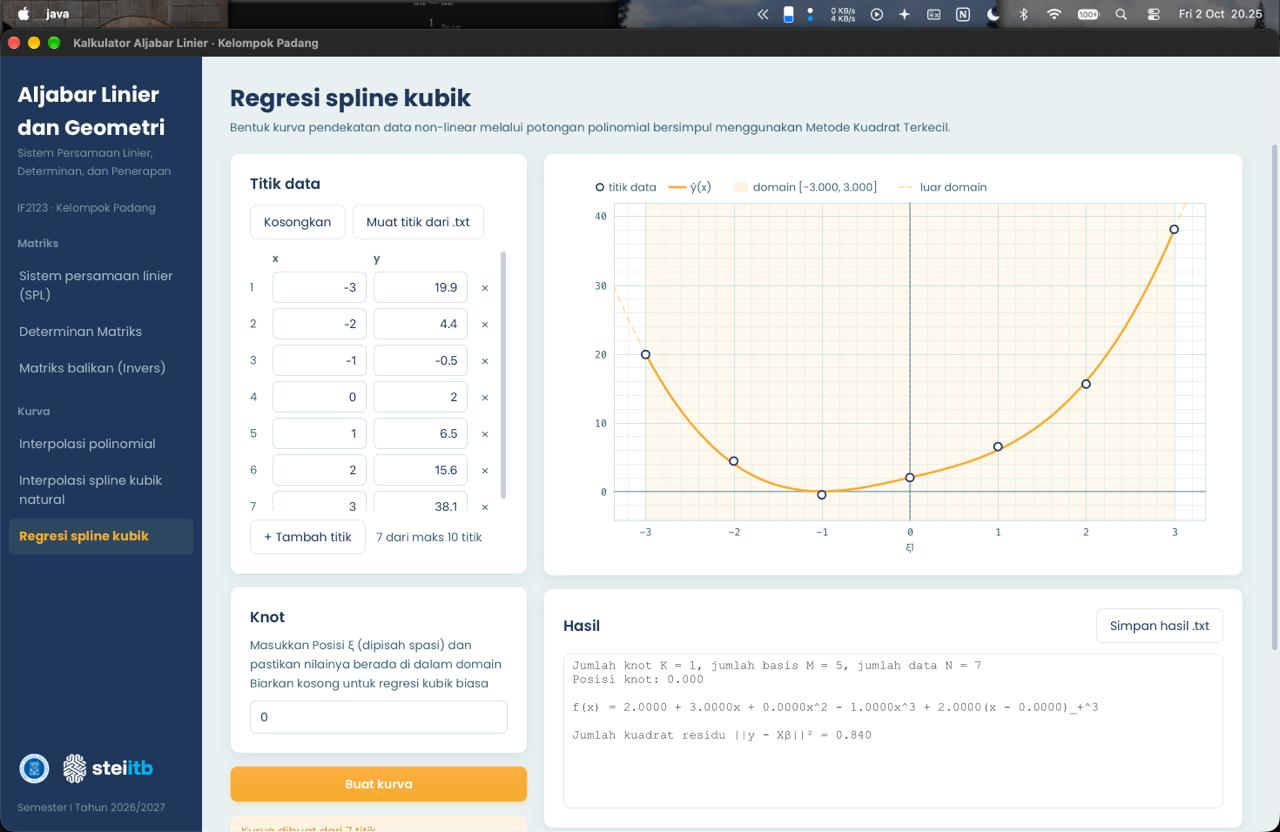
\includegraphics[width=0.8\textwidth]{regresi_spline_1.jpeg}
    \caption{Hasil Regresi Spline Studi Kasus 4.9.1}
\end{figure}

Program menghasilkan fungsi regresi
\begin{equation*}
    f(x) = 2 + 3x + 0x^2 - x^3 + 2\,(x-0)_+^3,
\end{equation*}
dengan jumlah kuadrat residual $\lVert \mathbf{y} - X\boldsymbol{\beta} \rVert^2 = 0{,}840$. Dalam bentuk piecewise:
\begin{equation*}
    f(x) =
    \begin{cases}
        2 + 3x - x^3, & x < 0, \\
        2 + 3x + x^3, & x \ge 0.
    \end{cases}
\end{equation*}

\begin{table}[H]
    \centering
    \begin{tabular}{|c|c|c|c|}
        \hline
        \textbf{$x$} & \textbf{$y$} & \textbf{$f(x)$} & \textbf{Residual} \\
        \hline
        $-3$ & $19{,}9$ & $20{,}0$ & $-0{,}1$ \\
        $-2$ & $4{,}4$  & $4{,}0$  & $0{,}4$ \\
        $-1$ & $-0{,}5$ & $0{,}0$  & $-0{,}5$ \\
        $0$  & $2{,}0$  & $2{,}0$  & $0{,}0$ \\
        $1$  & $6{,}5$  & $6{,}0$  & $0{,}5$ \\
        $2$  & $15{,}6$ & $16{,}0$ & $-0{,}4$ \\
        $3$  & $38{,}1$ & $38{,}0$ & $0{,}1$ \\
        \hline
    \end{tabular}
    \caption{Perbandingan Data Aktual dan Hasil Regresi Spline}
\end{table}

\textbf{Analisis:}
Kurva hasil regresi mengikuti pola data dengan sangat baik. Kurva turun dari $x=-3$ menuju titik minimum lokal di sekitar $x=-1$ (dengan $f(-1)=0$), kemudian naik semakin curam hingga $x=3$. Sisi kanan knot lebih curam karena suku $2(x-\xi)_+^3$ menambah kontribusi kubik hanya untuk $x \ge \xi$, sehingga koefisien $x^3$ berubah dari $-1$ (kiri knot) menjadi $+1$ (kanan knot).

Kesesuaian terhadap data ditunjukkan oleh residual yang kecil, dengan nilai mutlak maksimum $0{,}5$ dan jumlah kuadrat residual hanya $0{,}840$ untuk 7 titik data. Koefisien $x^2$ bernilai $0$, dan kurva tetap kontinu serta mulus ($C^2$) di knot $\xi=0$ karena menggunakan basis truncated power. Hal ini menunjukkan bahwa satu knot sudah cukup untuk menangkap perubahan kelengkungan data, dan penambahan knot kemungkinan hanya berisiko overfitting. Bagian kurva putus-putus di luar domain $[-3,3]$ merupakan ekstrapolasi dan kurang dapat diandalkan karena tidak didukung data.

% BAB 5: PENUTUP
\chapter{Penutup}

\section{Kesimpulan}

Tugas Besar Aljabar Linear dan Geometri telah berhasil mengimplementasikan berbagai konsep aljabar linear ke dalam sistem berbasis Java, meliputi perhitungan determinan, invers matriks, serta penyelesaian Sistem Persamaan Linear (SPL) dengan beberapa metode. Melalui tugas besar ini, diperoleh pemahaman mengenai penerapan konsep matematika ke dalam algoritma dan pemrograman berorientasi objek, sekaligus pengalaman dalam menyusun dokumentasi teknis menggunakan \LaTeX.

\section{Saran}

Pengembangan selanjutnya dapat difokuskan pada peningkatan interaktivitas pada bagian output sistem. Saat ini, hasil perhitungan masih ditampilkan secara statis sehingga pengguna hanya dapat melihat hasil akhir dari proses. Sistem dapat dikembangkan dengan menampilkan ilustrasi atau tahapan perhitungan secara bertahap, sehingga pengguna dapat memahami proses penyelesaian, bukan hanya memperoleh hasil akhirnya. Pengembangan ini diharapkan dapat meningkatkan aspek interaktif dan membantu pengguna dalam memahami penerapan setiap metode aljabar linear yang digunakan.

\section{Refleksi Anggota Kelompok}

\subsection*{Ghina Emelia Yantes (13525119)}
Selama mengerjakan Tugas Besar Aljabar Linear dan Geometri ini, saya menjadi makin paham dengan materi di kelas. Saya juga mempelajari materi baru pada penerapan interpolasi dan regresi kubik. Selain itu, saya juga belajar cara membuat GUI menggunakan Javafx yang menurut saya sangat menarik karena membuat saya mencoba lingkungan bahasa baru, yaitu Java. Hal lain yang yang saya dapatkan adalah bagaimana bekerja dengan tim dalam membuat sebuah project, bagaimana membagi tugas, koordinasi, dan sebagainya.
\subsection*{Sahla Nailah Salsabilla (13525134)}
Selama mengerjakan Tugas Besar Aljabar Linear dan Geometri ini, saya berfokus pada pengerjaan kode untuk susunan matriks dan operasi dasarnya, beserta invers dan determinan. Proses ini menuntut saya untuk memahami konsep Object-Oriented Programming (OOP) dalam Java agar kode yang saya buat untuk matriks dapat digunakan kembali (reusable) untuk berbagai ukuran matriks. Saya juga belajar format penulisan dalam LaTeX guna merancang struktur laporan yang rapi agar hasil kerja saya dapat dipahami dengan baik oleh pembaca.
\subsection*{Nayla Putri Ghaisani (13525140)}
Selama mengerjakan Tugas Besar Aljabar Linear dan Geometri ini, saya memperoleh berbagai pengalaman dan pengetahuan baru, khususnya dalam penerapan konsep \textbf{Object-Oriented Programming (OOP)} menggunakan bahasa pemrograman Java melalui penggunaan class dan objek. Selain itu, saya juga mempelajari penggunaan \textbf{LaTeX} untuk menyusun dan memformat laporan secara terstruktur, sistematis, dan rapi. Pengalaman ini tidak hanya membantu saya memahami materi yang dipelajari, tetapi juga meningkatkan kemampuan saya dalam mengimplementasikan konsep pemrograman serta menyusun dokumentasi teknis dengan baik.

\newpage 
\refstepcounter{chapter} 
\addcontentsline{toc}{chapter}{6 \quad Daftar Pustaka} \renewcommand{\bibname}{\thechapter \quad Daftar Pustaka}

\begin{thebibliography}{99} 
\setlength{\itemsep}{0.5em}

\bibitem{anton2010app}
H. Anton and C. Rorres, \textit{Elementary Linear Algebra: Applications Version}, 10th ed. Hoboken, NJ, USA: John Wiley \& Sons, 2010. [Online]. Available: \url{https://archive.org/details/ElementaryLinearAlgebraByHowardAnton10thEdition}

\bibitem{burden2011ch3}
R. L. Burden and J. D. Faires, \textit{Numerical Analysis}, 9th ed. Boston, MA, USA: Brooks/Cole, Cengage Learning, 2011, ch. 3 (Interpolation and Polynomial Approximation). [Online]. Available: \url{https://faculty.ksu.edu.sa/sites/default/files/numerical_analysis_9th.pdf}

\bibitem{muntingh2010}
G. Muntingh, ``Topics in Polynomial Interpolation Theory,'' Ph.D. dissertation, Centre of Mathematics for Applications, University of Oslo, Oslo, Norway, Dec. 2010. [Online]. Available: \url{https://www.researchgate.net/publication/265819309_Topics_in_Polynomial_Interpolation_Theory}

\bibitem{burden2011ch35}
R. L. Burden and J. D. Faires, \textit{Numerical Analysis}, 9th ed. Boston, MA, USA: Brooks/Cole, Cengage Learning, 2011, ch. 3, sec. 3.5 (Cubic Splines). [Online]. Available: \url{https://faculty.ksu.edu.sa/sites/default/files/numerical_analysis_9th.pdf}

\bibitem{deboor2001}
C. de Boor, \textit{A Practical Guide to Splines}, rev. ed. New York, NY, USA: Springer-Verlag, 2001. [Online]. Available: \url{https://doi.org/10.1007/978-1-4612-6333-3}

\bibitem{hastie2009}
T. Hastie, R. Tibshirani, and J. Friedman, \textit{The Elements of Statistical Learning: Data Mining, Inference, and Prediction}, 2nd ed. New York, NY, USA: Springer, 2009, ch. 5 (Basis Expansions and Regularization). [Online]. Available: \url{https://course.ccs.neu.edu/ds4420sp20/readings/ESLII.pdf}

\bibitem{james2021}
G. James, D. Witten, T. Hastie, and R. Tibshirani, \textit{An Introduction to Statistical Learning: with Applications in R}, 2nd ed. New York, NY, USA: Springer, 2021, ch. 7 (Moving Beyond Linearity). [Online]. Available: \url{https://www.statlearning.com/}

\bibitem{bertalmio2000}
M. Bertalmio, G. Sapiro, V. Caselles, and C. Ballester, ``Image Inpainting,'' in \textit{Proceedings of the 27th Annual Conference on Computer Graphics and Interactive Techniques (SIGGRAPH '00)}, New York, NY, USA: ACM, 2000, pp. 417--424. [Online]. Available: \url{https://doi.org/10.1145/344779.344972}

\bibitem{perez2003}
P. Pérez, M. Gangnet, and A. Blake, ``Poisson image editing,'' \textit{ACM Transactions on Graphics (TOG)}, vol. 22, no. 3, pp. 313--318, 2003. [Online]. Available: \url{https://doi.org/10.1145/882262.882269}

\end{thebibliography}
\newpage

\chapter{Lampiran}

\section{Repositori GitHub}
https://github.com/ghinayantes/algeo26-tb1-Padang.git

\section{Bonus LaTeX}
https://github.com/ghinayantes/algeo26-tb1-Padang/tree/main/docs/src

\section{Pernyataan Integritas Akademik}
Tugas ini disusun sepenuhnya tanpa bantuan kecerdasan buatan (\textit{Generative AI}), melainkan
hasil pemikiran dan analisis mandiri.

\vspace{1cm}
\begin{flushright}
\begin{minipage}{0.45\textwidth}
\centering


\includegraphics[width=4cm, height=1.5cm, keepaspectratio]{ttd1.png}\\[0.3em]
\textit{Ghina Emelia Yantes}

\vspace{0.8cm}


\includegraphics[width=4cm, height=1.5cm, keepaspectratio]{ttd2.jpeg}\\[0.3em]
\textit{Sahla Nailah Salsabilla}

\vspace{0.8cm}


\includegraphics[width=4cm, height=1.5cm, keepaspectratio]{ttd3.jpeg}\\[0.3em]
\textit{Nayla Putri Ghaisani}

\end{minipage}
\end{flushright}
\end{document}

